\documentclass[a4paper,12pt,ngerman]{article}

%%%%%% packages %%%%%%%%%
\usepackage{fancyhdr}
\usepackage{times}
\usepackage[utf8]{inputenc}
\usepackage[ngerman]{babel}
%\usepackage{fontspec}
\usepackage{helvet}
\usepackage{graphicx}
\usepackage{ngerman}
\usepackage[doublespacing]{setspace}
\usepackage{csquotes}
\usepackage[left=3.5cm, right=3cm, top=2.5cm, bottom=2cm]{geometry}
\usepackage{lscape}
\usepackage{graphicx}
\usepackage{subcaption}
\usepackage[leftcaption]{sidecap}
\usepackage{hyperref}
\usepackage{pythonhighlight}
\graphicspath{{./Abbildungen/}{./Abbildungen/detections/05,04,2021-15,39,10/}{./Abbildungen/graphs/}}


%\setmainfont{Arial}

%%%%%%pagestyle%%%%%%%%%
\setlength{\headheight}{15pt}
\pagestyle{fancy}
\fancyhead[R]{ }
\fancyhead[L]{\leftmark}

\rfoot{\thepage}
\cfoot{}
%%%%%%%%%%%%%%%%%%%%%

%%%%%%CODE%%%%%%

%%%%%%%%%%%%%%%

\begin{document}

	\begin{titlepage}
	\newgeometry{left=2cm, right=2cm, top=2cm, bottom=2cm}
	\begin{singlespace}
		\begin{center}	
			{\large Johannes-Gutenberg-Universität Mainz}\\
			\vspace{0.5cm}
			{\large Fachbereich 07 – Geschichts- und Kulturwissenschaften}\\
			\vspace{0.5cm}
			{\large Digitale Methodik in den Geistes - und Kulturwissenschaften}\\
			\vspace{1cm}
			{\large Wissenschaftliche Arbeit zur Erlangung des Master of Arts}\\
			\vspace{2cm}
			{\Huge Der Algorithmus als Betrachter \\ Computergestützte Erschließung der Plakatsammlung des Kunstmuseum Bayreuth}\\
			\vspace{2cm}
			{\large Betreuer: \\ Prof. Peter Bell \\ FAU Erlangen Nürnberg}\\
			\vspace{2cm}
		\end{center}
		\begin{flushright}
			{\large Mörfelden-Walldorf, den 04.05.2021}\\
			\vspace{0.5cm}
			{\large Autor: \\ Julius Emmel \\ Ludwigstraße 28 \\ 64546 Mörfelden-Walldorf}\\
			\vspace{0.5cm}
			{\large Tel: 0175 5144465 \\ Mail: julius.emmel@pm.me}
		\end{flushright}
	\restoregeometry
	\end{singlespace}
	\end{titlepage}

\newpage

%%% INHALTSVERZEICHNIS%%%
\thispagestyle{empty}
\tableofcontents

\newpage

%%%EINLEITUNG%%%
\section{Einleitung}
\subsection{Einführung in das Thema}
Diese Arbeit ist mit dem Ziel verfasst worden, den akademischen Grad des Master of Arts des Fachs der „Digitalen Methoden in den Geistes- und Kulturwissenschaften“, welches an der Johannes-Gutenberg-Universität in Mainz angeboten wird, zu erlangen. \\
Dieser Masterstudiengang hat es sich zum Ziel gesetzt, die geisteswissenschaftliche Gedankenwelt mit den Methoden der Informatik zu erschließen. In ihm können sich Geisteswissenschaftler*innen mit der modernen Informationstechnologie auseinandersetzen und die Möglichkeiten, die diese bietet, in ihr Fach tragen – ebenso öffnet er auch Informatiker*innen den Horizont für die Anwendung ihrer Fähigkeiten. \\
Konkret ermöglicht das Fach – welches im internationalen Sprachraum auch unter dem Namen „Digital Humanities“ gehandelt wird – Wissenschaftler*innen eine neue Herangehensweise an ihr bekanntes Fach.\footnote{Der Begriff der Digital Humanities im deutschsprachigen Raum ist durchaus ein wenig kritisch. Dies rührt daher, dass zum jetzigen Stand sich nicht alles unter diesem Begriff in Deutschland versammeln möchte, was auch international darunter zu verstehen ist. So bieten die Digital Humanities auch der Rechts- oder der Wirtschaftswissenschaft ein Zuhause, welche hier ihre eigenen Fächer bilden.}  So können Geisteswissenschaftler*innen klassische Pfade ihres Faches mit neuen Mitteln beschreiten und Fragestellungen bearbeiten, die vorher als viel zu aufwendig erachtet wurden. Ebenso eröffnet das Fach aber auch gänzlich neue Wege zu Fragestellungen, die ohne die Informationstechnologie sich nicht ergeben hätten. \\
Diese Arbeit trägt beide Teile in sich. Zum einen beschäftigt sie sich mit den Digitalisaten einer Kunstsammlung, die für die Wissenschaft zugänglich gemacht werden muss – Digitalisate, die ohne die Informationstechnik nicht existieren würden. Zum anderen soll die große Menge an Digitalisaten durch die Anwendung von Algorithmen und künstliche neuronale Netze überhaupt erst handhabbar gemacht werden.
Zur heutigen Zeit liegen große Teile von deutschen Kunstsammlungen nicht in digitaler Form vor. Sollte es einen digitalen Datensatz geben, muss dieser auch nicht mit dazugehörigem Bildmaterial ausgestattet sein und umfasst in vielen Fällen auch nicht die Gesamtheit der Sammlung. \\
Der Forschung entsteht dadurch das Problem, dass eine große Menge an Motiven einer breiten, wissenschaftlichen Öffentlichkeit nicht bekannt oder auch zugänglich ist. Daraus folgend können Fragen zu diesen Motiven nicht entstehen oder Fragen, die auf ähnliche Motive fußen, nicht gänzlich erörtert werden. Denn – und dieses Thema wird noch oft in dieser Arbeit angesprochen werden – nur auf einer gut strukturierten Datengrundlage kann auch eine gute wissenschaftliche Arbeit aufbauen. Darin unterscheidet sich die Geisteswissenschaft nicht von der Informatik. \\

\subsection{Erläuterung der Fragestellung}
Konkret möchte diese Arbeit sich mit einer in großen Teilen schon in Bildform vorliegenden Kunstsammlung widmen.\footnote{Nähere Ausführungen zum Datensatz selbst folgen in einem eigenen Teil}  Diese Sammlung ist in erster Linie in ihrer Digitalen Form ein Ordner voller Bilddateien. Diese Dateien sagen nichts über das Motiv, den Gestalter, die Zeit oder andere klassifizierende Merkmale der Plakate als solches aus. Die Datei liefert lediglich Informationen zu sich selbst und dem Scan, den sie beinhaltet. Ein zusätzliches Dokument in Form einer CSV- oder XML-Datei liegt dem Datensatz auch nicht bei. \\
Für die Kunstgeschichte ist mit diesem Datensatz in der Form nichts gewonnen. Sie bietet kaum einen Mehrwert, der von Wissenschaftler*innen in einer Form genutzt werden kann. \\
Das Ziel dieser Arbeit ist es dies zu ändern und möglicherweise ein Verfahren zu schaffen, das auf andere Sammlungen dieser Art anwendbar ist. In diesem Sinne ist das erste Ziel dieser Arbeit in verkürzter Form die Erstellung von Metadaten für die einzelnen Scans der Sammlungsobjekte. Diese Metadaten bilden die durchsuchbare Grundlage, die von Anfragen an die Sammlung auf Motive schließen lässt. \\
Die Form der Metadaten ist dabei nicht klar definiert. In der simpelsten Anforderung sollen beschreibende Daten von mehreren einzelnen Worten entstehen. Diese Worte können die einzelnen Objekte in ihrem Motiv, der Aussage des Objektes oder den durch sie vermittelten Informationen beschreiben.\footnote{In unserem konkreten Fall sprechen wir von Plakaten. Diese besitzen in den meisten Fällen ein Motiv und Schrift, die dem Betrachter Informationen vermitteln möchten. Aus diesen Informationen lässt sich dann eine Aussage erschließen. So möchte beispielsweise ein Plakat mit der Abbildung eines Kunstwerks und der Nennung von einem Museum und einem Zeitraum mit großer Wahrscheinlichkeit auf eine Ausstellung aufmerksam machen.}  In einer anspruchsvolleren Form können diese Metadaten auch aus kurzen Sätzen bestehen, welche einen Aufschluss darüber geben, was das Plakat dem Betrachter zu vermitteln versucht. \\
Ermöglichen soll diese Generierung von Metadaten ein neuronales Netz. Dieses soll nach dem Training ihm unbekannte Plakate in wichtige Bildelemente unterteilen können. So soll es beispielsweise erkennen welche entscheidenden Motive und Texte es beinhaltet. Aus diesen erkannten Bildmerkmalen sollen dann Informationen extrahiert werden, die dann als Metadaten dienen. \\
Neben der Durchsuchbarkeit einer Sammlung kann auch ihre Präsentation ein entscheidender Erkenntnisgewinn sein. Die einfache Ordnerstruktur gibt wenig Aufschluss darüber, was in den eigentlichen Bilddateien zu sehen ist. Durch Clusteringverfahren auf Basis von visuellen Features ist es jedoch möglich bildliche Ähnlichkeiten zu finden und die Dateien entsprechend in einem mehrdimensionalen Raum anzuordnen. Auch dieser Annäherungsversuch soll im Rahmen dieser Arbeit unternommen werden. \\

\subsection{Besprechung des Datensatzes}
Das Quellen- beziehungsweise Datenmaterial dieser Arbeit entstammt dem 20. Jahrhundert und der Sammlung des Kunstmuseums Bayreuth. Dieses Beherbergt seit 2012 die von Dr. Franz-Joachim Schultz seit 1986 zusammengetragenen Plakate. Seinen Bestand von 16.000 Plakaten konnte das Museum Bayreuth mittlerweile auf über 18.000 Plakate erweitern.\footnote{Vgl. Kunstmuseum Bayreuth, Plakatsammlung (12.10.2020).} \\
Der Datensatz enthält konkret 15.351 Digitalisate. Diese tragen Namensbezeichnungen wie „fünfzehn1\_007“ und geben ansonsten keine weiteren Hinweise auf das Plakat, das der Scan zeigt. Viele dieser Abbildungen sind auch Doubletten, wodurch sich eine genaue Zahl von einzigartigen Motiven nicht genau angeben lässt. \\
Die Abbildungen selbst reichen in ihren Motiven, Formaten und Themengebieten von Flyern zu Büchern und Programmbroschüren bis hin zu Veranstaltungs- und Werbeplakaten in Formaten zwischen DIN A4 bis DIN A0 – und darüber hinaus. In einem anderen Teil dieser Arbeit soll auch noch auf einzelne Plakate eingegangen werden und beispielhaft an diesen erläutert werden, wo die Herausforderungen bei der Arbeit mit Plakaten liegen. \\

\subsection{Die Struktur der Arbeit}
Diese Arbeit unterteilt sich in einen theoretischen und einen praktischen Teil. Im theoretischen Teil soll zuerst auf die Gattung des Plakats in der Kunstgeschichte eingegangen werden. Hier wird in einer verkürzten Form auf die Wandlung der Gestaltung und die Ansprache der Betrachter*innen eingegangen werden. \\
In einem weiteren Abschnitt soll dann auf den Datensatz als solchen im Detail eingegangen werden. Hier sollen einzelne Beispiele aus dem Datensatz besprochen werden. Der Fokus der Betrachtung liegt dabei auf den Anforderungen, die die Plakate an die Technik stellen – welche Vorgehensweisen vom Programmierer erwogen werden können und welche Maßnahmen sich auf die Arbeit und das Endergebnis wie auswirken können. \\
Abgeschlossen wird dieser Teil mit einer Wiedergabe von drei Gesprächen, die mit Vertreter*innen dreier deutscher Museen geführt wurden. Sie erläutern aus ihrem Alltag die Probleme, die sie in Bezug auf die Erschließung ihrer Sammlungen erlebt haben, was für Herausforderungen sie auch speziell im Kontext der Plakatsammlungen sehen und welche Schritte notwendig wären, um in Deutschland die Digitalisierung von Plakaten voranzubringen. \\
Im technischen oder auch praktischen Teil der Arbeit soll dann zunächst auf die verwendete Technik eingegangen werden. Hierbei stehen die Technologie und ihre Verwendung im Vordergrund. \\
Darauffolgend wird der eigene Umgang mit dieser Technologie beschrieben und wie sich die konkrete Entwicklung ergeben hat. Exemplarisch werden auch Teile des Codes besprochen und gezeigt, welche Problemlösungen und Herangehensweisen gewählt wurden. \\
Am Ende der Arbeit steht die Vorstellung der erzielten Ergebnisse, deren Auswertung, sowie der Ausblick auf die sich daraus ergebenden Perspektiven. \\

\newpage

\section{Plakatkunst}
\subsection{Die Geschichte des Plakats}
Um den Anfang der Geschichte des Plakats zu setzen bedarf es zunächst einer Definition, was man unter dem Begriff Plakat überhaupt versteht. \\
Sieht man im Plakat vor allem die Hauptaufgabe der Wissens- und Informationsvermittlung an öffentlichen Wänden, so können schon Graffitos aus der Antike als erste Plakate in Betracht gezogen werden.\footnote{Döring: Anfänge des Plakats (2020), S. 20.}  „Erklärt man das Plakat allerdings als ein gedrucktes Blatt Papier, das, von Weitem sichtbar, für etwas wirbt, dann liegen seine Anfänge in den Jahren um 1800.“\footnote{Ebd., S. 20.}  Dieser doch recht klare Zeitraum ergibt sich für Döring aus dem Kontext der französischen Revolution. Ihre Revolutionär*innen hätten sich über das vorherrschende Primat des Staates, als einzigem Verfasser von öffentlichen Bekanntmachungen, hinweggesetzt und ihre revolutionären Botschaften mittels Plakaten der breiten Masse zugänglich gemacht. Nach der französischen Revolution habe es dann im Zuge der weiteren Revolutionen auf dem europäischen Kontinent immer wieder neue Anstiege in der Auflagenzahl von Plakaten gegeben.\footnote{Ebd., S. 20/21.} \\
Hellmut Rademacher setzte den Beginn von Plakaten in das 15. Und 16. Jahrhundert, wobei zu dieser Zeit das Flugblatt eine deutlich stärkere Auflagenzahl gehabt haben dürfte – vom gestalterischen Gesichtspunkt her habe es kaum Unterschiede gegeben. Öffentliche Aushänge hätten dabei „Ankündigungen von Theaterstücken, Menagerien, Verlosungen, Schützenfesten, reisenden Künstlern, Scharlatanen, Ärzten, Kurpfuschern“ zum Inhalt.\footnote{Rademacher: Das deutsche Plakat (1965), S. 12.}  Laut Rademacher stammt „das älteste bekannt deutsche Theaterplakat aus Rostock, aus dem Jahre 1520.“\footnote{Rademacher: Theater Plakate (1989), S. 12.} \\
Generell ist eine klare Benennung eines Anfangs zusätzlich erschwert, da das Plakat ein Medium des stätigen Wandels ist und die einzelnen Blätter selten für einen längeren Gebrauch gedacht sind – im Falle von Veranstaltungsplakaten besitzen sie am Tag nach dem beworbenen Ereignis nicht mehr den ihnen angedachten informatorischen Wert.\footnote{Döring: Anfänge des Plakats (2020), S. 20; Rademacher: Theater Plakate (1989), S. 7.} \\
Die treffendste Definition kommt wohl von Martina Lückerath, wenn sie schreibt:


\blockquote{\fontsize{10pt}{12pt}\selectfont Vorstufen dazu gab es zwar schon seit dem Altertum, als öffentliche Bekanntmachungen oder unerlaubte Beschriftungen auf Wände und Mauern geschrieben wurden, und seit Gutenbergs Erfindung des Buchdruckverfahrens mit beweglichen Lettern um 1450 entstanden nicht mehr nur Informationsblätter für den gezielten Anschlag an vielbesuchten Stätten, sondern auch gedruckte Handzettel und Flugblätter, die in größerer Stückzahl verteilt wurden. […] Die technischen und sozialen Voraussetzungen für das moderne Plakat entwickelten sich jedoch erst seit etwa 1830, um das anspruchsvoll gestaltete künstlerische Plakat entstand überhaupt erst im letzten Drittel des 19. Jahrhunderts.\footnote{Lückerath: Galerie der Straße (1998), S. 11.}}


Während Döring das vermehrte Aufkommen an Plakaten auch durch die Revolutionen und das damit verbundene Bedürfnis der Bevölkerung nach freier Meinungsäußerung erklärt, liegt der Fokus bei Rademacher viel stärker auf der sozialen und ökonomischen Notwendigkeit von Menschen und Firmen ihre Produkte an den Mann und die Frau zu bringen.\footnote{Rademacher: Das deutsche Plakat (1965), S. 12-14.}  Lückerath sieht diese Entwicklung auf eine ähnliche Weise und führt, wie Rademacher, das rasante Städtewachstum im 19. Jahrhundert als Argument an.\footnote{Ebd., S. 16; Lückerath: Galerie der Straße (1998), S. 12.}  Zusammenfassend erkennt sie, dass das Plakat auch das Erzeugnis von, „durch gesellschaftliche[n] und wirtschaftliche[n] Veränderungen verschärfte[m,] Konkurrenzdruck“ sei.\footnote{Lückerath: Galerie der Straße (1998), S. 12.} \\
Zusammen mit diesem immer größeren Bedürfnis von Akteur*innen, wie Handwerker*innen oder Schausteller*innen, um das Werben von Aufmerksamkeit in einer stetig wachsenden Stadtbevölkerung, profitiert das Plakat auch von technischem Fortschritt. So wurde ab 1844 Papier aus Holzschliff gefertigt, was dessen Preis deutlich senkte.\footnote{Ebd., S. 11.} Zudem wurde ab 1815 die, Lithographie als Drucktechnik immer bekannter.\footnote{Ebd., S. 11.}  „Die in den Jahren 1796 bis 1798 von Alois Senefelder erfundene Lithographie, [welche] von ihm selbst anfangs als chemische Druckerei bezeichnet [wurde] […]. Mit ihr wurde es fortan möglich, zu billigem Preise große Auflagen in beliebigen Formaten zu drucken.“\footnote{Rademacher: Das deutsche Plakat (1965), S. 16.} Ab 1827 wurde durch die Chromolithographie auch der Vielfarbendruck möglich und durch das Einführen von Zinkblechwalzen am Ende des 19. Jahrhundert, konnte eine massenweise Produktion von Plakaten ermöglicht werden.\footnote{Für eine genauere Beschreibung der Entwicklung der Lithographie um 1900 eignet sich auch der Beitrag von Hirt-Tenger, vgl. Hirt-Tenger: Entwicklung und Techniken der Lithographie (2016); Lückerath: Galerie der Straße (1998), S. 11; Rademacher: Theater Plakate (1989), S. 14.} \\ 
Diese vielen Plakate mussten auch einen Platz im städtischen Raum gewinnen, der für sie bis dahin nicht vorgesehen war.\footnote{Für Rademacher hat dieses Fehlen von Anschlagflächen auch die verspätete Verbreitung von Plakaten in Deutschland zur Folge, vgl. Rademacher: Das deutsche Plakat (1965), S. 17.}  Das führte in den frühen Jahren des 19. Jahrhunderts zu einer wilden Plakatierung in den großen europäischen Metropolen und brachte Erfindungen wie die Plakatsäule in London 1824, Paris 1842 und Berlin 1855 hervor.\footnote{Lückerath: Galerie der Straße (1998), S. 12.}  Aber auch im Innenraum oder in Schaukästen an Häuserwänden, wurde mit Plakaten geworben.\footnote{Döring: Anfänge des Plakats (2020), S. 21; Döring: Plakat im Jugendstil (2020), S. 64.} \\
In der Literatur wird allgemein Jules Chéret als erster großer Revolutionär in der Plakatwelt gehandelt. Er eröffnet 1866 seine Druckerei in Paris, nachdem er sich zuvor in England aufgehalten hat.\footnote{Döring: Plakat im Jugendstil (2020), S. 64; Rademacher: Das deutsche Plakat (1965), S. 24-26., Lückerath: Galerie der Straße (1998), S. 12.}  In seiner Druckerei entstanden neben anderen Erzeugnissen auch Plakate, welche er selbst entwarf.\footnote{Döring: Plakat im Jugendstil (2020), S. 64.} \\
Chéret entwickelte das Plakat zum einen technisch weiter, in dem seine Plakate wetterbeständiger waren und so auch besser im freien überdauern konnten. Ebenso begann er ab 188/89, mittels der Farblithographie, mit den drei Grundfarben Rot, Blau und Grün zu drucken. Zum anderen dachte er aber auch das Plakat von einer gestalterischen Perspektive neu. So soll er der erste gewesen sein, der Text und Bild miteinander zu verknüpfen wusste.\footnote{Döring: Plakat im Jugendstil (2020), S. 64; Rademacher: Das deutsche Plakat (1965), S. 24-26.} \\
Chéret präsentiert seine Werke auch auf der Weltausstellung 1889 in Paris, was Döring als Ausgangspunkt für den Plakat Boom in den 1890er Jahren in Paris sieht – Laut Lückerath erreicht diese, auch als „affichomanie“ bezeichnete, Begeisterung für das Plakat 1894 ihren Höhepunkt.\footnote{Für Rademacher ist es viel mehr der „Durchbruch des Impressionismus in den achtziger Jahren [des 19. Jahrhunderts]“, vgl. Rademacher: Das deutsche Plakat (1965), S. 21; Döring: Plakat im Jugendstil (2020), S. 64; Lückerath: Galerie der Straße (1998), S. 13.}  Neben Chéret sind es „die Plakate von Grasset, Willette, Bonnard, Steinlen, Mucha und insbesondere diejenigen von Toulouse-Lautrec [die] dem Medium Plakat den Rang eines eigenständigen Kunstwerks“ in dieser Zeit verleihen.\footnote{Lückerath: Galerie der Straße (1998), S. 13.}  Dies wird auch durch die Gründung des „Salon des Cent“ im Jahr 1894 befördert, in welchem Plakate neben angewandter und freier Kunst präsentiert werden.\footnote{Döring: Plakat im Jugendstil (2020), S. 64.} \\
Ausgehend von Paris beginnt sich das Plakat ab 1894 dann auch in England und in den vereinigten Staaten immer mehr durchzusetzen.\footnote{Lückerath: Galerie der Straße (1998), S. 13; Döring: Plakat im Jugendstil (2020), S. 65.}  In Festlandeuropa dauert diese Entwicklung länger.\footnote{Döring: Plakat im Jugendstil (2020), S. 65.} \\
In Deutschland spielte das Plakat eine gewisse Doppelrolle vor der Jahrhundertwende. Dies war auch, laut Rademacher, dadurch bedingt, dass „die offizielle akademische Kunst in Deutschland […] vom Staat und von den kulturellen Ambitionen der herrschenden Klassen gefördert [wurde] und […] von ihnen abhängig“ war.\footnote{Rademacher: Das deutsche Plakat (1965), S. 54.}  So gab es kein vergleichbares Aufkommen von Künstlerplakaten wie in Frankreich. Auf der anderen Seite galt „die Plakatwand als Galerie auf der Straße, als Kunstausstellung für den sogenannten kleinen Mann – das wurden Schlagworte der Zeit“ nach Rademacher.\footnote{Rademacher: Deutsche Plakatkunst und ihre Meister (1965), S. 11; Lückerath: „Galerie der Straße“ (1998), S. 16.}  Dieses Bewusstsein dafür, dass Plakate auch Kunstwerke sind und künstlerische Werte vermitteln können, schlägt sich auch in den ab 1893 beginnenden Ausstellungen und Plakatsammlungen in deutschen Museen nieder.\footnote{Purcell: Das Museumsplakat als Designgeschichte (2018), S. 13; Lückerath: „Galerie der Straße“ (1998), S. 15.}  Erst nach der Jahrhundertwende sieht Lückerath, dass „Gebrauchsgraphiker und Kritiker […] sich nun entschieden gegen den Gedanken einer ästhetischen Erziehung durch die ‚Galerie der Straße‘ [wandten]. Das sich als formal eigenständiger Aufgabenbereich der Gestaltung durchsetzende Plakat entzog sich zunehmend dem Vergleich mit der Bildkunst.“\footnote{Lückerath: „Galerie der Straße“ (1998), S. 16.} \\
Mit der Jahrhundertwende setzt immer mehr eine Professionalisierung des Plakats als Medium ein. Künstler erhalten feste Verträge mit Druckereien, zudem werden neue Ausbildungsstätten in Form der Gewerbeschulen geschaffen, in denen sich Menschen zu Werbezeichnern ausbilden lassen können.\footnote{Döring: Halbzeit der Moderne (2020), S. 122; Lückerath: „Galerie der Straße“ (1998), S. 19.} \\
Ebenso gibt es Umstrukturierungen im Entstehungsprozess der Plakate. So nahmen sich ab 1905 in den USA Werbeagenturen der Konzeption von Kampagnen an und trennten diese personell von den Firmen, die zuvor eigene Abteilungen oder Graphiker beschäftigten.\footnote{Döring: Halbzeit der Moderne (2020), S. 123.} \\
Neben den Kreativen, wird auch an das Plakat selbst neue Maßstäbe gesetzt. Es wird zunehmend verwissenschaftlicht und Aspekte wie die Ansprache des Betrachters und das schnelle Vermitteln der Inhalte werden wichtiger.\footnote{Ebd., S. 123.} \\
Im Zuge dieser Entwicklung entsteht in Deutschland das sogenannte deutsche Sachplakat um 1905. Dabei handelt es sich um ein Werbeplakat, welches sich durch einen einfarbigen Hintergrund, vor dem das beworbene Produkt zu sehen ist, auszeichnet. Textlich wird dem Motiv oft nicht mehr als der Firmenname beiseitegestellt. Sein wohl bekanntester Vertreter ist der Grafiker Bernhard.\footnote{Döring: Halbzeit der Moderne (2020), S. 123; Purcell: Das Museumsplakat als Designgeschichte (2018), S. 14; Lückerath: „Galerie der Straße“ (1998), S. 17.} \\
Mit dem ersten Weltkrieg bildet sich dann auch eine weitere große Themengruppe – Das politische Plakat.\footnote{Döring: Halbzeit der Moderne (2020), S. 123; Lückerath: „Galerie der Straße“ (1998), S. 18.}  Wurde zuvor vor allem für Sach- und Dienstleistungen, sowie Veranstaltungen und Ausstellungen mit Plakaten geworben, so kam nun auch der Wettbewerb um politische Ideen hinzu. Es ist hierbei anzumerken, wie Döring auch schon mit seinem Verweis auf die Französische Revolution zeigt, dass Plakate zuvor keineswegs unpolitisch waren. Vielmehr professionalisiert der erste Weltkrieg als starke politische Auseinandersetzung dieses Themengebiet im Zuge des aktuell herrschenden Zeitgeistes.

\blockquote{\fontsize{10pt}{12pt} \selectfont Politische Kampfplakate anlässlich von Wahlen oder harte ‚Ja-Nein‘-Kampagnen bei Volksabstimmungen wie in der Schweiz waren im wilhelminischen Deutschland verpönt und oft sogar verboten worden. […] Es fehlte den Plakatkünstlern an Praxis auf politisch kontroversen Arbeitsfeldern. Dazu mussten die Künstler Neuland außerhalb der gewohnten Entwürfe für Industrie und Export, für Konsum und Luxus, für Reisen und Sport betreten.\footnote{Krause: Einleitung (2015), S. 11.}}

Zusammen mit Dörings Ausführungen zur französischen Revolution ist es dann auch nachvollziehbar, wieso sich in anderen europäischen Nationen das politische Plakat leichter tat.\footnote{Döring: Anfänge des Plakats (2020), S. 20-21; Krause: Einleitung (2015), S. 11.} \\
Die im deutschen Sachplakat erkennbare Orientierung hin zur Vereinfachung in der Plakatgestaltung wird nach dem ersten Weltkrieg in der Avantgarde fortgeführt. In den 1920er und 30er Jahren ist sie laut Döring an einer geraden und serifenlosen Schrift, sowie klaren, rechteckigen Flächen in Verbindung mit schwarz-weiß Fotografie zu erkennen. Die bekannteste Strömung der Avantgarde sei die des Art déco, welche ihre Ursprünge bereits vor dem großen Krieg findet, jedoch in den 20ern zu ihrer Hochform gelangt.\footnote{Döring: Art déco und Avantgarde (2020), S. 160.} \\
Der zweite Weltkrieg wird allgemein in der Literatur eher als Zeit der Stagnation bezeichnet – man scheint sich noch wenig mit dieser Zeit beschäftigt zu haben.\footnote{Hier sei auf das Buch Geklebte NS-Propaganda von Birgit Witamwas verwiesen. Sie beschäftigt sich ausführlich mit dem Plakat im zweiten Weltkrieg, vgl. Witamwas: Geklebte NS-Propaganda (2016); Lückerath: „Galerie der Straße“ (1998), S. 19.}  Die Zeit danach wird dann als Phase der Wiederanknüpfung an die Vorkriegszeit und als gleichzeitige Neuausrichtung in die Zukunft verstanden. Ursächlich für diese Entwicklung ist sicherlich auch die Tatsache, dass die aktiven Grafiker nach dem Krieg auch schon vor dem Krieg tätig waren und somit selbst vor der Herausforderung standen sich mit ihrem alten Wissen neu zu erfinden.\footnote{Kühnel: Werbegrafik in Deutschland seit 1945 (2016), S. 20-25.} \\
Ein Stil, der sich nach dem Krieg herausbildet, ist der Schweizer oder auch Schweizer typografische Stil.\footnote{Döring: Nach dem Zweiten Weltkrieg (2020), S. 210.}  „Flächige Farben, Fotografie, eine rasterbasierte Anordnung von Typografie und die ausschließliche Verwendung von Groteskschriften sind die prägenden Elemente“\footnote{Zeller: World Wide Willisau (2017), S. 9.} \\
Ein entgegengesetzter Ansatz ist die Verwendung von handgezeichneten Motiven und Typographien, wie sie unter anderem in der polnischen Plakatschule anzutreffen ist.\footnote{Döring beschreibt verkürzt auch einen stilistischen Unterschied zwischen den beiden politischen Blöcken nach dem zweiten Weltkrieg – einen technischeren, reduzierteren Stil im Westen und einen verspielteren, handgemachten Stil im Osten. Die Diversität des Ostplakats am Beispiel der DDR-Filmplakate bietet Detlef Helmbold, vgl. Helmbold: Mehr Kunst als Werbung (2018) und Döring: Art déco und Avantgarde (2020), S. 161; Döring: Nach dem zweiten Weltkrieg (2020), S. 210; Lückerath: „Galerie der Straße“ (1998), S. 20.} \\
Ein weiterer Aspekt in der Professionalisierung des Plakatwesens ist das Abhalten von regelmäßigen Wettbewerben. Im deutschsprachigen Raum kam es 1941 zum ersten Wettbewerb unter dem Namen der „besten Schweizer Plakate des Jahres“. Ab 1945 suchte die Handelskammer Mannheim nach dem besten Deutschen Plakat der Wirtschaftswerbung.\footnote{Bei Wettbewerben gilt es dabei zu unterscheiden zwischen Wettbewerben, mit deren Gewinn auch die Vergabe eines Auftrags in Verbindung steht und Wettbewerben, die es sich zum Ziel gesetzt haben, die beste gestalterische Leistung in einem Zeitraum zu küren, vgl. Müller: Best german posters (2016), S. 2.}  Im Zusammenhang mit diesen Wettbewerben gründeten sich auch neue Berufsverbände, wie der „Bund Deutscher Gebrauchsgraphiker“ oder der „Art Directors Club Deutschland“, die als Ausrichter solcher Wettbewerbe auftraten.\footnote{Ebd., S. 2; Döring: Pop und Poster (2020), S. 259.} \\
Auch das Künstler*innenplakat erlebt nach dem zweiten Weltkrieg eine erneute Beliebtheit. Angefangen mit Plakaten von Picasso 1948 entdecken immer mehr Pariser Künstler*innen das Medium für sich. Dieser Aufschwung kam 1960 auch in den New Yorker Galerien an.\footnote{Döring: Nach dem Zweiten Weltkrieg (2020), S. 211; Lückerath: „Galerie der Straße“ (1998), S. 20.}  Durch die Nähe zur Kunstszene kommt es auch wieder zu einer stärkeren Durchmischung von Inspirationsquellen – So können Musikcover, Kunstrichtungen wie die Pop-Art oder andere Plakate Ideen für neue Motive und Gestaltungsweisen liefern.\footnote{Döring: Pop und Poster (2020), S. 258; Grohnert: Sand fürs Getriebe (2018), S. 93; Lückerath: „Galerie der Straße“ (1998), S. 21.} \\
Mit dem Wiedererstarken des Künstler*innenplakats wird das Plakat vor allem ab den 1970er Jahren wieder zu einem Sammlerstück – auch für Privatpersonen.\footnote{Ebd., S. 258.}  In Postershops können Plakate aus aller Welt erworben werden. Im Zuge der 68er Bewegung werden Sie auch zum Ausdruck der eigenen politischen Haltung.\footnote{Grohnert: Sand fürs Getriebe (2018), S. 94.}  Anders als beim politischen Plakat, welches zuvor meist von Parteien bespielt wurde, steht hier der Protest und die Unzufriedenheit mit der politischen Lage im Vordergrund. Protestplakate bedienen sich meist provokanten Motiven und Sprüchen und wollen den Betrachter zum Nachdenken anregen. Einer ihrer bekanntesten Vertreter ist Klaus Staeck.\footnote{Ebd., S. 93; Döring: Pop und Poster (2020), S. 258-259.} \\
Seit jeher steht das Plakat nicht nur in Konkurrenz zu anderen Plakaten, sondern auch zu anderen Werbeträgern.\footnote{Grohner: Sand fürs Getriebe (2018), S. 97.}  Ab den 1980er Jahren beginnt auch das Internet als zu bewerbender Raum hinzuzukommen. Zunächst bringt der PC, über das es verbreitet wird, die Möglichkeit von digitalen Gestaltungstools und Druckmethoden mit.\footnote{Ebd., S. 97, Döring: Globalisierung (2020), S. 304-305.}  Hiervon profitiert das Plakat auch und gewinnt abermals an Diversität. \\
Die Literatur ist sich einig, dass das Auftreten der Digitalisierung der Werbung und des Internets dem Plakat auf lange Dauer eher geschadet hat.\footnote{Grohnert sagt in einem Bezug auf Klaus Staeck auch, dass dessen Plakate in Zeiten des dezentralen Internets untergehen würden. Das dies nicht zwangsweise der Fall sein muss zeigt Staecks Versuch das Internet als Vertriebsweg für seine Plakate zu nutzen, vgl. Grohnert: Sand fürs Getriebe (2018), S. 99; Staeck, Plakatshop (28.02.2021); Purcell: Das Museumsplakat als Designgeschichte (2018), S. 18.}  In den digitalen Raum hinein kann es nicht wirken. Dort wird in anderen Formaten und mit einer größeren Aufdringlichkeit geworben. René Grohnert fasst es in dem Sinne zusammen: „Es wurde auf die eine Eigenschaft reduziert, die es einmalig macht: seine Präsenz im öffentlichen Raum. Man kann Plakate nicht wegklicken oder ausschalten, man bleibt ihnen ausgesetzt.“\footnote{Ebd., S. 97.}  Aber der digitale Raum schafft es auch durch große Computerbildschirme als Werbeflächen in den Lebensraum des Plakats einzudringen – die animierte Werbung hält somit auch Einzug in die analoge Welt. \\
Das Plakat steht als Werbemittel seit seinen Anfängen unter ständigem Konkurrenzdruck. Es muss sich gegen Kleinwerbemittel und Bewegt-bildanzeigen und seinen Platz in der städtischen Landschaft ständig behaupten. Durch sein grafisches Erscheinungsbild, sein Format und die Akteure, die es bespielen, drängt sich stets der Vergleich zur bildenden Kunst auf. Die enorme zeitliche Ausrichtung, der auch eine Kurzlebigkeit in der inhaltlichen Bedeutsamkeit inhärent ist, verwehrt ihm jedoch diesen Status. Die Zeiten, in denen das Plakat prosperierte, waren auch immer Zeiten des wirtschaftlichen Aufstiegs. Dabei ist es unerheblich, welches Wirtschaftssystem gerade das Vorherrschende ist – eine gewisse werbliche Konkurrenz, der Bedarf an Aufmerksamkeit, ist immer gegeben. Als Medium der Masse ist es dafür konzipiert mit einer großen Anzahl Rezipient*innen zu interagieren und zugleich in einer großen Zahl selbst vertreten zu sein. Diese beiden Faktoren – das Ansprechen eines großen Publikums und das Sprechen aus einer großen Menge – haben zur Folge, dass das Plakat auch in einer entsprechend großen Zahl auftreten muss. Es lebt von seiner Diversität und Individualität. Technischer Fortschritt hat dabei stets geholfen seine Mannigfaltigkeit in Erscheinung und Zahl zu steigern, doch das Digitale ist zusätzliche Konkurrenz und enormes Potential zugleich – es bietet dem Plakat die Chance, sich selbst gestalterisch weiterzuentwickeln und in eine digitale Form zu transformieren, dabei besetzen digitale Werbeflächen hart erkämpften Werbeplatz der Plakate. Seine Geschichte zeigt aber auch, dass zusätzliche Konkurrenz kein Nachteil für das Plakat ist.

\newpage

\subsection{Herausforderungen der Bilderkennung – An Beispielen aus der digitalen Plakatsammlung Bayreuth}
In der Einleitung wurden bereits die Eckdaten der Bayreuther Plakatsammlung benannt. Im nun folgenden Teil soll genauer auf Plakate im Allgemeinen am Beispiel dieser Sammlung eingegangen werden.\footnote{Die Auswahl der Plakate basiert auf der subjektiven Entscheidung des Autors und einer einfachen, stichprobenartigen Durchsicht des Datensatzes. Es besteht die Chance, dass für die genannten Beispiele besser geeignete Alternativen im Datensatz vorhanden sind und das bei einer weiteren Durchsicht des Datensatzes eine andere Auswahl an Beispielen getroffen würde.} Im Fokus steht hier die Besprechung darstellerischer Besonderheiten des Mediums Plakat und wie diese sich auf die Leistung von Bilderkennungsalgorithmen auswirken können. \\
Zunächst soll aber das Plakat als solches genauer Besprochen werden. Dies dient auch dazu, Definitionen zu schaffen, die es ermöglichen Plakate von einem Algorithmus in eben diese einordnen zu lassen.\footnote{Durch die enorme Heterogenität von Plakaten, können diese Definitionen nicht auf alle Plakate einer Kategorie in Gänze zutreffen. Auch die Anzahl an Definitionen muss auf andere Sammlungen nicht zutreffen – es wurde sich bemüht möglichst generelle Definitionen der einzelnen Plakatklassen zu geben.} \\ 
Ein Plakat dient in erster Linie der Wissens- und Informationsvermittlung.\footnote{Döring: Anfänge des Plakats (2020), S. 20.}  Helmut Rademacher beschreibt die Grundsätzliche Funktion eines Plakats so:

\blockquote{\fontsize{10pt}{12pt} \selectfont Mit einem Blick muß sein in Wort und Bild zum Ausdruck gebrachter Inhalt erfaßbar sein, in Blitzeseile muß es dem Betrachter seine Losung oder seinen Slogan ins Gesicht schleudern, muß es ihm seine Aussage in konzentrierter Form wie im Telegrammstil vor Augen führen, ohne durch zu starke Komprimierung der Aussage diese nur bruchstückhaft, ungenügend und dadurch vielleicht sogar falsch oder unverständlich erscheinen zu lassen.\footnote{Rademacher: Das deutsche Plakat (1965), S. 7.}}

Gerade diese von Rademacher beschriebene „Komprimierung der Aussage“ ist für die Bilderkennung eine Herausforderung, da der erkennende Algorithmus zunächst nur die Information aus dem Plakat ziehen kann, die darauf explizit ausgewiesen ist. Weggelassene Zusammenhänge und das Voraussetzen von, für die Entstehungszeit des Plakats, relevanter Hintergrundinformation besitzt der Algorithmus nicht.
Je nach dem Kontext, in dem das Plakat steht, handelt es sich um andere Formen von Information. \\

\subsubsection{Das Ausstellungsplakat}
Bewirbt das Plakat eine Ausstellung ist das Thema der Ausstellung die erste Wichtige Information, die es vermitteln muss. Mit einer Hohen Wahrscheinlichkeit ist das Thema, der Grund, weswegen sich der Betrachter die Ausstellung schlussendlich anschauen wird. Das Thema wird meist in Motiv und Text vermittelt. Die zweite wichtige Information ist die ausrichtende Institution. Sie ist durch ihren Namen und ihr Logo zu erkennen. In manchen Fällen besitzt eine Institution ein Corporate Design, welches ebenfalls auf sie verweist. Die dritte wichtige Information des Ausstellungsplakat ist der Zeitraum der Ausstellung und die Öffnungszeiten des Ausstellungshauses und ist ein ebenso wichtiges Kriterium, ob die Ausstellung besucht wird. Nebeninformationen sind Logos von Sponsoren der Ausstellung, Informationen zu Ticketpreisen oder Kontaktdaten der Institution (Abb. 1). \\

\subsubsection{Das Programmplakat}
Ein Programmplakat bewirbt in der Regel mehrere einzelne Veranstaltungen, die im Kontext eines größeren, sie überspannenden, Themas stehen. Der Veranstaltungszeitraum kann dabei zwischen einem Tag, einem Wochenende und mehreren Wochen variieren. Sowohl das Thema als auch die Zeitangabe sind die Hauptinformationen, die das Programmplakat vermitteln muss. Im Gegensatz zum Ausstellungsplakat ist der beworbene Zeitraum viel fragmentierter. Gegebenenfalls variieren Veranstaltungsort und Zeitraum der einzelnen Veranstaltungen. Ebenso können inhaltliche und konzeptionelle Unterschiede bestehen. All diese Abweichungen müssen dementsprechend auf dem Plakat repräsentiert sein. In Sonderfällen kann das Programm nur in Auszügen gezeigt und dann auf einen Webauftritt verwiesen werden. Generell lässt sich sagen, dass ein Programmplakat meist reich an Text ist und so mit dem Motiv, welches auf das Hauptthema Bezug nimmt, in ein Spannungsverhältnis tritt. Oftmals kann ein Motiv aber auch gänzlich fehlen oder durch verzierende Ornamentik ersetzt werden. Die Nebeninformationen entsprechen denen des Ausstellungsplakats (Abb. 2). \\

\subsubsection{Das Veranstaltungsplakat}
Im Gegensatz zu Ausstellungs- und Programmplakat wirbt das Veranstaltungsplakat nur für ein Event an einem bestimmten Abend oder Tag – in Sonderfällen kann auch ein längerer Zeitraum, etwa ein Wochenende, benannt werden. Zum Inhalt hat es daher ein konkretes Thema. Oft sind die handelnden Personen und die Form der Veranstaltung genauer benannt. Neben dem Thema, das auch wieder das Motiv beeinflusst, sind der Ort und die Zeit wichtige Informationen, die das Plakat vermitteln muss. Sonderfälle können sogenannte Eindruckplakate sein. Diese besitzen eine feste Form für wiederkehrende Elemente – wie Veranstaltungsorte oder die ausrichtende Organisation. Sie besitzen Leerstellen in ihrer Komposition und können so beispielsweise für einzelne Abende in einer Veranstaltungsreihe werben. In diesen Fällen kann das Motiv auch auf die Organisation oder die Veranstaltungsreihe selbst verweisen. Auch Sponsoren können als Nebeninformation auf Veranstaltungsplakaten abgedruckt sein (Abb. 3, 4 und 5). \\

\subsubsection{Das politische Plakat}
Eine weitere Plakatform, die auf ein bestimmtes Datum hin wirbt, ist das politische Plakat. Zumindest dann, wenn das Plakat im Kontext eines Wahlkampfs steht. Unabhängig von diesem Kontext geht es dem politischen Plakat aber immer darum den Betrachter von den auf den Plakaten angebrachten Botschaften in Bild und Schrift zu überzeugen – und im Kontext des Wahlkampfes an einem bestimmten Tag sein Kreuz bei der entsprechenden Partei zu machen. Ein politisches Plakat besteht aus einem Motiv und einer verschriftlichten Botschaft. Es weist gegebenenfalls auf einen Wahltermin hin und trägt das Logo der veröffentlichenden Partei (Abb. 6) Eine zweite Form des politischen Plakats ist Partei unabhängig und kann von Privatpersonen und Nichtregierungsorganisationen (NGOs) veröffentlicht sein. Diese wollen meist mit dem Plakat auf Missstände und Themen aufmerksam machen, die von der parlamentarischen Politik ihrer Meinung nach nicht gut genug behandelt werden (Abb. 7). \\
In diesem Kontext soll noch ein gestalterischer Sonderfall erwähnt sein. In der Bayreuther Plakatsammlung lassen sich zehn Plakate der Reihe „Plakatdebatte“ des Vereins „Partnerschaft 3. Welt und Tür an Tür – miteinander leben e. V.“ finden. Bis auf die gleiche Fußzeile haben die Plakate die gestalterische Eigenart, sehr viel unbedruckte Fläche auf sich zu tragen. Im oberen Fünftel des Plakats drängen sich mehrere Zeilen Text, die politische und gesellschaftliche Themen der Zeit aufgreifen und in provokante Aussagen gießen. In der unteren, linken Ecke, aber auch teilweise mit direkten Fragen an den Betrachter wird dieser dazu ermutigt mit dem Plakat zu interagieren und seine eigene Meinung zu dem vom Plakat aufgeworfenen Thema aufzuschreiben. Somit wird das Plakat nicht nur Sender von Botschaften, sondern auch zum Empfänger und Mittler weiterer, von den Betrachtern beigetragenen Inhalten (Abb. 8). \\
\\
Allen bisher benannten Plakatgruppen ist die Eigenschaft gemein, dass sie auf ein bestimmtes Datum hinweisen. Sie besitzen ein Verfallsdatum, das den von ihnen vermittelten Inhalt danach nicht mehr so dringlich erscheinen lässt – Wenn der letzte Ausstellungstag vorbei ist, wird man diese Ausstellung nicht mehr besuchen können, wenn die Wahlbüros geschlossen sind, können die umworbenen Wähler*innen ihre Stimme nicht mehr abgeben.\\
Dieses Problem tragen die folgenden Plakatgruppen nicht so eindeutig auf sich selbst. Auch sie besitzen eine Aktualität und wirken in einem Zeitraum am besten auf die ihnen angedachte Art und Weise. Dieser Zeitraum lässt sich aber nicht so klar benennen und kann auch über ein abgedrucktes Datum hinaus gehen. \\

\subsubsection{Das Filmplakat}
Am klarsten tritt dies im Filmplakat in Erscheinung. Auf diesem wird mit einem Motiv aus dem Film oder den Bildern der Schauspieler*innen in den Hauptrollen geworben. Es trägt den Titel des Films, die Namen der Darsteller*innen und oftmals auch eine Liste an weiteren beteiligten Personen. Haben Regisseur*in oder Produzent*in bereits größere Erfolge an der Kinokasse erzielt, werden ihre Namen oder diese Filme genannt, um einen zusätzlichen Werbeeffekt auszulösen. Ebenfalls werden die Logos der Produktionsfirmen gezeigt. Zumeist werden diese Plakate in die Öffentlichkeit gebracht, wenn der Film, den sie bewerben noch nicht erschienen ist. Somit werben Sie auf ein Datum hin, anstatt auf etwas, dass an dem Datum enden wird. Wann diese Verfügbarkeit endet, liegt nicht mehr in der Macht des Plakats und seiner Erschaffer, sondern bei den zeigenden Institutionen (Abb. 9). \\

\subsubsection{Das Theaterplakat}
Das Theaterplakat ist in gewissem Sinne eine Mischung aus Film und Veranstaltungsplakat. Es kündigt meist eine serielle Veranstaltung an, die aber nur in einer begrenzten Häufigkeit, einer Saison, gezeigt wird. Wie beim Filmplakat werden der Titel des Stücks und die bei der Produktion beteiligten Personen genannt. Ebenso wird auf das Schauspielhaus und die Aufführungstermine verwiesen – diese können aber auch weggelassen sein. Gegebenenfalls treten auch Sponsoren auf (Abb. 10). Eine Trennung von Kultur und Werbeplakaten erscheint auch in Hinblick auf Kühnels Aussage

\blockquote{\fontsize{10pt}{12pt} \selectfont Marketingstrategien stehen über einem künstlerischen Anspruch. Die sich bereits in den 1960er-Jahren angekündigte Trennung von Kultur- und Wirtschaftswerbung hat längst ihren sichtbaren Ausdruck in den Städten bekommen, wo eigens eingerichtete Kultursäulen vermietet werden.\footnote{Kühnel: Werbegrafik in Deutschland seit 1945 (2016), S. 114.}}

und ihrer Beobachtung, dass im Bereich des Kulturplakats noch am ehesten Selbstständige und kleinere Grafikbüros anzutreffen seien, sinnvoll. Interessant wäre in diesem Zusammenhang, ob eine computergestützte Analyse des Datensatzes eine Unterscheidung zwischen Theater- und Filmplakaten, beziehungsweise Kultur- und Werbeplakaten auch nahelegen würde. \\

\subsubsection{Das Produktplakat}
Das Produktplakat bewirbt einen Gegenstand oder eine Dienstleistung, die von einem Unternehmen oder einer Organisation produziert oder angeboten wird. Das Motiv nimmt darauf Bezug. Textlich werden dem Produkt sein Name und gegebenenfalls beschreibende Sätze beiseitegestellt, sollte das Motiv noch nicht hinreichend auf das Produkt aufmerksam gemacht haben oder wenn sich bestimmte Aspekte des Produkts nicht in Bildern darstellen lassen. Neben dem Produktnamen sind auch der Name der Firma und ihr Logo wichtig, sollten beide nicht übereinstimmen. Eine Zeitangabe ist bei Produktplakaten sehr selten, da die Plakat-Kampagne meist mit der Marktveröffentlichung des Produkts startet oder das Produkt auch schon längere Zeit am Markt vorhanden ist (Abb. 11). \\

\subsubsection{Das Buchplakat}
Die Kategorie des Buchplakats ist eine Sonderform des Produktplakats. Es ist jedoch so auffällig in der Bayreuther Sammlung vertreten, dass es geboten erschien, es gesondert zu erwähnen. In vielen Fällen zeigt das Buchplakat lediglich das Cover des Buches, das es vermarktet (Abb. 12). Darüber hinaus kann auch das gesamte Buch mit Auszügen aus Rezensionen, einem Autor*innenbild und Angaben zum Preis und der Seitenzahl gezeigt werden. Auffällig ist beim Buchplakat, dass es hier auch zu hochrechteckigeren Plakatformen kommen kann, die in anderen Plakatkategorien so nicht oft anzutreffen sind (Abb. 13). \\
\\
Dieser erste Teil der Plakatanalyse anhand der Bayreuther Plakatsammlung wird im späteren Verlauf der Arbeit, in Bezug auf eine Visualisierungsmethode mit Hilfe von \textit{Machine Learning}, wichtig. Denn um eine maschinelle Unterscheidung von Plakaten zu erreichen, bedarf es zunächst einer klaren Definition. Die hier benannten acht Kategorien sind aber nicht allumfassend und in der Bayreuther Plakatsammlung lassen sich Beispiele finden, die sich nicht als Plakat identifizieren lassen oder zu wenige Anhaltspunkte bieten, um klar in eine der Kategorien eingeordnet zu werden (Abb.14 und 15). \\
Im zweiten Teil soll nun auf gestalterische Einzelheiten von Plakaten eingegangen werden. Neben den verschiedenen Merkmalen, die sich auf Plakaten finden lassen, liegt der Fokus besonders auf Überlegungen zu möglichen Problematiken in der Gestaltung. Diese werden wichtig, wenn es um den Aspekt der \textit{Object Detection} geht. Gegliedert ist dieser Abschnitt dabei in die Bereiche „Schrift“, „Grafik“, „Schrift-Grafik-Verschränkungen“ und „Scans“. \\
Ebenfalls sind einigen Plakaten in diesem Abschnitt Bilder beiseitegestellt, auf denen von einem neuronalen Netz klassifizierte Bildelemente zu sehen sind. In den Fällen, in denen das Netz keine Anmerkungen auf den Plakaten gemacht hat, wurde auf eine Wiederholung des Bilds verzichtet.\footnote{Dieser Arbeit liegt auch ein digitaler Ordner bei, der die Bilder des Abbildungsteils, sowie ihre annotierten Versionen beinhaltet. Zudem befinden sich weitere Bilder in diesem Ordner als ergänzendes Material.}  Nähere Ausführungen zum Annotationsprozess der Bilder werden im späteren Verlauf der Arbeit gemacht. \\

\subsubsection{Schrift}
Die eindeutigste Informationsquelle auf Plakaten ist in aller Regel die Schrift. Sie zeigt in klaren Worten an, was das Plakat bewirbt und in welchem Zeitraum seine hauptsächliche Aktualität liegt. Dies gilt besonders, wenn die Schrift in Textblöcken auftritt und keine zu starke Verbindung von Motiv und Schrift vorliegt. Das Schriftbild, die Fonts, sind für sich ebenfalls ein kritisches Feld. So tritt Schrift, schon gar nicht über verschiedene Plakate hinweg, im gleichen Font auf – aber auch auf sich selbst kann ein Plakat verschiedene Schriften tragen (Abb. 16). Die Schwierigkeit für den Computer besteht dabei nicht die Schrift als solche zu erkennen, vielmehr würde sich in anschließenden \textit{Optical Character Recognition} (OCR) Prozessen dann die Problematik ergeben, aus den unterschiedlichen Schriftbildern auch sauber erkannte Daten-Strings zu erzeugen. Vor dem Hintergrund, dass mit einem Bilderkennungsalgorithmus auch Tags für die entsprechenden Bilder erzeugt werden sollen, ist die OCR Erkennung in jedem Fall unabdingbar und somit eine Belieferung der Software mit ordentlichen Textausschnitten erforderlich. Wie in Abbildung 17 zu sehen ist, erkennt das für die Annotationen verwendete neuronale Netz zwar den Vogel auf dem Plakat, die Schrift und andere Bildelemente nimmt es jedoch nicht wahr. \\
Die Text-Ausschnitte sind mitunter schwer zu erstellen, da mit der Einbeziehung der Schrift in das Motiv des Plakats eine Verfremdung des Schriftbildes einhergeht. Eine solche Verfremdung kann das Entzerren der einzelnen Worte sein. Am Beispiel des Veranstaltungsplakats „Torsten Zwingenberger – Im Podium \& Band“ wird das Wort „Band“ im Titel in seine einzelnen Buchstaben aufgeteilt (Abb. 18). Diese werden dann übereinander angeordnet. Mit einer großen Wahrscheinlichkeit wird der Algorithmus hier die einzelnen Buchstaben erkennen und diese jeweils einzeln an die OCR Software weiterreichen. In diesem Fall muss im Anschluss an die OCR Erkennung geprüft werden, ob nur einzelne Buchstaben erkannt werden und gegebenenfalls müssen diese dann zu einem Wort zusammengesetzt werden. Hier ist wiederum entscheidend, dass die Software auch erkennt, welcher Buchstabe wo im Plakat auftaucht und koordinatenbezogen eine Hierarchie zwischen den Buchstaben herstellt. Alternativ könnte auch über einen Thesaurus abgeglichen werden, ob bestimmte Kombinationen der Buchstaben sinnvolle Worte ergeben. Bei diesem Ansatz müsste noch geprüft werden, welches, sollten mehrere Worte in Frage kommen, dann auch auf dem Plakat steht. In anderen Fällen können diese beiden Ansätze unvorhergesehene Fehler produzieren und gegebenenfalls unbrauchbar sein. \\
Eine weitere, gravierendere Veränderung kann die Auflösung der einzelnen Buchstaben zum Zweck der Bildgestaltung sein. Im Fall des „Festival für internationale Gegenwartskunst“ werden die Wörter „subvision.“, „kunst.“ und „festival.“ durch Punkte in einem Raster angedeutet (Abb. 19). Für das menschliche Auge ergeben sich aus den verschiedenen Punkten bei genauerem Hinschauen die Wörter, die Maschine wird darin jedoch nur schwer einen Sinn erkennen können. Durch das Auftauchen der Worte in anderen Textabschnitten, kann der Kontext des Plakats dennoch rekonstruiert werden. Problematisch wird es, wenn sich Wörter auf dem Plakat nicht wiederholen und unleserlich für die Maschine sind. Wortwiederholungen hingegen können durch entsprechende Abgleiche zwischen den aus den Plakaten gelesenen Strings vermieden werden. Ähnliche Schwierigkeiten sind auf dem Ausstellungsplakat „Mythos Berlin“ zu sehen (Abb. 20). Hier verschmelzen die Buchstaben „S“ und „B“ zu einem. Für den Betrachter erschließt sich der Sinn, die Maschine wird aus der neu geschaffenen Glyphe jedoch wenig Sinn ziehen. Wie auch beim vorher genannten Plakat wird die Schrift im Motiv auch in einem lesbareren Schriftsatz wiederholt. Es stellt sich die Frage, wie das Schrift-Motiv im Plakatzentrum kategorisiert werden soll, sollte es nicht als Text erkannt werden. Denkbar wäre es ebenfalls für die Verbindung von Schrift und Motiv eine eigene Kategorie zu finden, die in ein eigenes Schlagwort überführt werden kann. Fraglich bleibt dann, ob für diesen Fall entsprechendes und ausreichendes Trainingsmaterial für den Algorithmus gesammelt werden kann und ob diese neue Kategorie sich scharf genug vom reinen Text-Label abgrenzen lässt. Auf dem Plakat des Senders Freies Berlin (SFB) in der Reihe „Musik der Gegenwart“ werden die Buchstaben in ihrer Form gestreckt und gestaucht und somit auch die Zeilenstruktur gebrochen (Abb. 21). Für den Algorithmus ergibt sich hier das Problem, dass er die Worte „Arnold Schönberg“ und „Gurrelieder“ nur schwer auseinander halten können wird. Selbst wenn er die beiden unteren zwei Drittel des Plakats als Textblock erkennt, würde dann die OCR Software mit großer Wahrscheinlichkeit daran scheitern. \\
Auch die Größe der Schrift kann zum Problem werden. Auf den ersten Blick scheint die Erkennung der Bildelemente bei dem Plakat mit einem Peanuts Motiv einfach (Abb. 22). Die Schrift in der Sprechblase ist gut zu lesen und auch vom restlichen Motiv abgegrenzt. Dieses wiederum ist eine einfache Zeichnung des Hundes Snoopy auf dem Dach seiner Hundehütte. Bei genauem Hinsehen lässt sich eine Impressumszeile in der linken, unteren Ecke des Plakats entdecken. Sie beinhaltet wichtige Informationen zum Jahr, den Auftraggeber*innen und dem Ort. Ihre Größe könnte im Training des neuronalen Netzes problematisch werden. Hier kommt es darauf an, mit welcher Größe man die Bilder dem Algorithmus vorlegen kann. Bei einer zu großen Verkleinerung kann aus der Zeile schnell eine Schwarze Linie werden oder sie kann ganz verschwinden. Auch beim Klassifizieren des Plakats kann es zu Problemen kommen. Sollte der Ausschnitt der Schrift nur verschwommene Buchstaben zeigen, wird die OCR Software keine Wörter daraus lesen können. Wichtiger Faktor bei einer so kleinen Schrift ist daher die Qualität des Scans bei starker Vergrößerung. Auch eine unterschiedliche Größe der Buchstaben in einem Wort kann zu Problemen führen. In einem weiteren SFB Plakat in der Reihe „Musik der Gegenwart“ werden die Buchstaben „i“, „n“, „t“, „K“, „e“, „n“ und „D“ jeweils in einer anderen Größe als die Restlichen Buchstaben ihrer Wörter geschrieben (Abb. 23). Auch hier ergibt sich das Problem, das sich bei den entzerrten Buchstaben des Wortes „Band“ gezeigt hat – die Wörter können gegebenenfalls nicht als eins erkannt werden. Auch kann dies der Sonderfall sein, der den Lösungsvorschlag für Abbildung 18 erschwert, wenn nicht gar unbrauchbar macht. Würden hier alle einzeln erkannten Buchstaben zusammengefügt werden, würde sich kein sinnvolles Wort ergeben. \\
Ein letztes mögliches Problemfeld im Gebiet der Schrift sind unterschiedliche Zeichensysteme. In der Sammlung des Bayreuther Plakatmuseums treten asiatische und arabische Schriftzeichen und Lautschrift auf (Abb. 24-26). Das Hauptproblem sollte sein, dass der Bilderkennungsalgorithmus in den verschiedenen Schriftzeichen Text erkennt und diesen entsprechend ausschneiden kann. Die OCR Software sollte dann unabhängig von der Sprache eine Übersetzung in Strings vornehmen können. Für den Algorithmus bietet es sich möglicherweise an, für andere Zeichensysteme ein eigenes Label zu besitzen. Dies würde eine weitere Unterscheidungsebene in die Plakate bringen und den Trainingsdatensatz für Schrift und Text stärker gliedern – Es würden somit nicht lateinische und andere Zeichen in einem Label vertreten sein, was möglicherweise auch zu besseren Ergebnissen führen kann. \\

\subsubsection{Grafik}
Das zweite große Element eines Plakats ist das Motiv, das es trägt. Es dient als der hauptsächliche Blickfang und soll den Betrachter auf das Thema des Beworbenen hinweisen oder den Publizierenden zu erkennen geben. Um die aufsehenerregende Wirkung des Plakats zu steigern und sich aus dem großen Feld an konkurrierenden Druckerzeugnissen hervorzutun, sind für das Motiv keine Grenzen gesetzt. So können gezeigte Objekte und Personen verfremdet oder abstrahiert, Bildelemente können gezielt weggelassen oder verstellt werden. Auf eine möglichst einprägsame Weise muss genau so viel Information vermittelt werden, dass der Betrachtende sich in einem flüchtigen Moment dazu hingerissen fühlt, mehr vom Plakatinhalt entdecken zu wollen. \\
Ein Mittel dafür ist die Verzerrung von gezeigten Objekten. Das Plakat zum Kostümfest der Hochschule für bildende Künste Berlin zeigt das Gesicht einer jungen Frau (Abb. 27). Durch die Schrift auf ihrem Gesicht deutet sich an, dass das Bild von ihr etwas in die Länge, nach oben hin, gezogen ist. Farblich ist das Plakat in Rottönen gehalten. Für die Bilderkennung stellt sich in so einem Fall die Frage, ob die Verzerrung des Bildgegenstandes sich negativ auf seine Erkennbarkeit auswirkt. Ebenfalls kann die Farbvarianz zu Irritationen führen. Wie die nebenstehende Annotation von Abbildung 27 zeigt, hat das neuronale Netz in diesem Fall mit einer 60\%igen Wahrscheinlichkeit ein Stoppschild in der Frau gesehen – vermutlich wegen der Schrift und dem Rotton. Ein neuronales Netz ist im Normalfall auf Abbildungen von Personen trainiert, die der Wirklichkeit ähneln. Durch eine andere Farbgebung können gelernte Prinzipien getäuscht werden. Entsprechende Schritte im \textit{Preprocessing} der Trainingsdaten, der Bildmanipulation vor dem Training, könnten zu besseren Ergebnissen, aber auch zu einer vollkommenen Verwirrung des Netzes führen. Es würde sich auf jeden Fall um einen sehr starken Eingriff in das Bildmaterial handeln, der in sehr feinen Abstufungen durchgeführt werden müsste. Auf dem amnesty international Plakat gegen die Todesstrafe ist die Verzerrung noch deutlicher (Abb. 28). Hier erkennt das untrainierte Netz keinen Menschen. \\
Ein stärkeres gestalterisches Mittel ist die Verfremdung von Motiven. Das Werbeplakat einer Stadtbücherei zeigt beispielsweise eine Kreatur, die sehr stark einem Hund ähnelt (Abb. 29). Die Verfremdung äußert sich neben der Farbe vor Allem im Kopf des Hundes. Dieser ist ein Buch, welches sich zur langen Schnauze formt. Ein Lesebändchen deutet sowohl die Zunge als auch die Leine des Hundes an. Der Körper des Tiers ist in warmen Farbtönen von Violett bis Gelb gestreift. Algorithmen, die vor allem an den Fotografien von Hunden trainiert sind, werden mit sehr großer Wahrscheinlichkeit Probleme haben dieses Tier als Hund zu identifizieren. Dies zeigt auch die Annotation dieses Plakats durch das neuronale Netz. Zwar kennt es die Kategorien Hund und Buch, klassifizieren kann es keinen dieser Gegenstände in diesem Mischwesen – die drei Objekte, die es findet, sind Drachen im Körper, den Vorderpfoten und dem rechten Ohr. Wie in einem späteren Absatz dieses Teiles noch näher zu erörtern ist, stellt sich auch die Frage, ob man dieses Wesen überhaupt als Hund labeln möchte. \\
Eine ähnliche Verfremdung, bestehend aus der Kombination verschiedener Objekte, kann man auch bei dem Plakat für die „Biennale of Illustrations Bratislava“ sehen (Abb. 30). Abgebildet ist eine Zeichnung von Dušan Kállay die sich aus der vorderen Hälfte eines Löwen und den Beinen eines Vogels zusammensetzt. Dieses Mischwesen ist bekleidet mit einem Hut, einer Brille und Teilen einer Ritterrüstung. Farblich sind die Beine und der Schild, sowie eine umgehängte Tasche nicht ausgefüllt. Mit einem entsprechend gut auf Tiere trainiertem Algorithmus könnten die einzelnen Teile noch erkannt werden, was die Annotationen auch bestätigen. Interessant ist, dass er jeweils die komplette Figur mit der Kategorie „bird“ und „dog“ benennt und sich tendenziell sicherer zu sein scheint, dass es sich um einen Vogel handelt. Aber auch hier stellt sich die große Frage des korrekten Labels. Möchte man die Einzelteile des Tieres erfassen oder ist das eindeutigere Merkmal als Mischwesen das entscheidende. Bei letzterem besteht die Problematik der möglicherweise unzureichend vorhandenen Trainingsdaten. Zudem wäre diese Kategorie sehr heterogen, was eine klare Klassifizierung erschweren würde. \\
Das Veranstaltungsplakat zum „Festival International des Francophonies“ schmückt ein anderes Tier (Abb. 31). In Anspielung an den Titel des Festivals „Drôles des Zebres“ wird ein nach hinten blickendes Zebra im Profil gezeigt. Sein Kopf wird zu seinem Hinterteil hin drei Mal wiederholt. Wie es zu erwarten ist, erkennt der Algorithmus hier mehrere Zebras – zwei von vier möglichen. Problematisch wird dies, wenn man im Anschluss an die Erkennung der Bildinhalte auch eine Erfassung der Anzahl der erkannten Bildelemente machen möchte – was in anderen Fällen durchaus eine wünschenswerte Mehrerkenntnis wäre. Unabhängig von der erkannten Anzahl der Zebras, würde hier ebenfalls die Verfremdung des Zebras nicht miterkannt. \\
Nahezu unmöglich wird die Bilderkennung, wenn das Dargestellte den Bereich des Figürlichen verlässt. Im Ausstellungsplakat des Museum Zirndorf, dem Veranstaltungsplakat zur Kinderbuchmesse in Bologna und dem Werbeplakat der Edition Hoffmann wird dies anschaulich (Abb. 32-34). Die drei Plakate zeigen eine abstrakte Drahtskulptur, eine Zusammenstellung unterschiedlicher Hölzer und Farben, sowie eine Raute aus unterschiedlich spitzzulaufenden, senkrechten Linien. Beim ersten Beispiel könnte noch ein Label wie Skulptur greifen, jedoch bleibt es schwer vorzustellen, dass ein Algorithmus in dem Knäul aus Draht auch eine Skulptur erkennt. Auch die leichte Holzstruktur in den einzelnen Farbflächen bleibt mit großer Wahrscheinlichkeit unerkannt. Das untrainierte Netz erkennt keinerlei Bildinhalte auf den drei Plakaten. Gerade diese Beispiele zeigen, wie limitiert die Bilderkennungsalgorithmen hier noch sind und wie wichtig es ist klare Definitionen für Bildinhalte zu finden. Dies muss der erste Schritt sein, bevor überhaupt entsprechendes Trainingsmaterial gesammelt und vorbereitet werden kann. \\
Das Problem der Abstraktion leitet über auf ein weiteres, welches sich aus der Darstellung von Kunstwerken ergibt. Auf dem Ausstellungsplakat zum Danner Preis von 1990 ist ein solches in der Form einer elliptischen Skulptur vor schwarzem Hintergrund abgebildet (Abb. 35). Denkbare Label Kategorien wären Begriffe wie „Ring“, „Kunstwerk“ und „Skulptur“. Sie alle beschreiben das gesehene in einer unterschiedlich starken Abstraktion. Der Begriff „Ring“ trifft es zwar am genauesten von der puren Form des gezeigten, jedoch geht hierbei die gesamte Ebene des Kunstwerks in diesem Label verloren. In dieses Label würden sich schlussendlich Ringe und Kreise jeglicher Form einordnen lassen. Das Label „Kunstwerk“ beschreibt das Objekt hingegen unabhängig von seiner Form, als etwas kreativ vom Menschen Geschaffenes. Aber auch dieses Label würde viel mehr einschließen und Medien wie Malerei, Grafik, Fotografie und zu einem gewissen Grad auch Architektur umfassen. Eine Kategorie viel zu divers, als dass ein Algorithmus hier ein klares Muster erkennen könnte. Der Begriff der „Skulptur“ scheint daher am zutreffendsten, jedoch ist auch das Feld an Skulpturen in sich enorm divers. So kann es einfache, runde Objekte wie auf diesem Plakat geben und, ebenfalls aus vielen Rundungen bestehende, Drahtskulpturen wie auf Abbildung 32. Neben den Abstrakten Skulpturen kommen dann auch figürliche Statuen hinzu, die zur Diversität beitragen, jedoch auch noch eine ganz andere Problematik mitbringen. Die Ausstellungsplakate zur Dauerausstellung der mährischen Galerien in Brünn und zur Werkschau von Sylva Lacinová sind zwei Beispiele für figürliche Bildinhalte (Abb. 36 und 37). Das Plakat zur Ausstellung „Sylva Lacinová“ zeigt eine sitzende Figur. Ihre Ellenbogen hat sie auf ihren Beinen abgestützt und in den Händen hält sie eine Art Frucht, möglicherweise einen Apfel. Nicht nur passt diese Figur nicht zu einem Label, das abstrakte Skulpturen beschreiben soll – obwohl es sich eher um eine stilisierte Darstellung des menschlichen Körpers handelt – auch trifft das Label des „Menschen“ oder der „Person“ den Bildinhalt nicht vollkommen. Das neuronale Netz tut sich ebenfalls schwer und wählt Begriffe wie „Vase“ und „Teddybär“. Ein guter Zwischenweg wäre ein Label „Abbild des Menschen“. Dieses würde auch auf die Figur des Plakats aus Brünn zutreffen. Die dortige Detailaufnahme einer größeren Skulptur aus drei weiblichen Figuren aus Bronze zeigt eine dieser Figuren von nahem. Es handelt sich hierbei klar um das Abbild eines menschlichen Körpers, welches dennoch nicht vom Netz erkannt wird. Vielmehr sieht er im Pflanzenornament zur Rechten der Figur einen Hund. \\
Das Problem setzt sich in der Zeichnung fort. Die Ausstellungsplakate zu Henry Moore des Rupertinum in Salzburg und zur tschechischen Kunst des 20. Jahrhunderts in den mährischen Galerien Brünn, sowie das politische Werbeplakat zum Frauenstreik 1991, zeigen Zeichnungen von humanoiden Körpern (Abb. 38-40). Das neuronale Netz erkennt nur im Plakat zur Henry Moore Schau überraschenderweise eine Person. In dem Plakat aus Brünn kann es nichts erkennen und im Streikplakat sieht es einen Regenschirm. Im Falle der Figur von Henry Moore wäre das Label des „Mensch“ als interpretationswürdig einzuschätzen, gerade daher erstaunt die Zuschreibung durch das Netz. \\
Diese Beispiele aus Skulptur und Zeichnung machen deutlich, wie wichtig eine klare Benennung von Bildinhalten ist. Im konkreten Fall bedarf es einer klaren Unterscheidung von lebenden Menschen, Abbildern von Menschen und nicht figürlicher Kunst. Dabei muss eindeutig benannt werden, ab wann es sich nur noch um das Abbild eines Menschen handelt – denn genau genommen fängt dies schon bei der Fotografie eines Menschen an. Wichtig ist hierbei, dass die Linie zwischen realen Menschen und ihren Abbildern deutlich wird. Ein Label für beides wird bei zunehmendem Abstraktionsgrad zu ungenau für einen Computeralgorithmus. Wird die Kategorie jedoch zu eng gefasst, könnte sich schnell eine Vielzahl an Unterkategorien ergeben, die eine entsprechende Menge an eindeutigem Trainingsmaterial erforderlich machen. \\
Eine weitere Problematik, die auch schon für die Schrift angesprochen wurde, ist die Kleinteiligkeit, die auch die Bilderkennung beeinflussen kann. Auf den Werbeplakaten für die „Graswurzelrevolution“ und die Buchreihe „Berlin Crime“ vom Verlag edition monade finden sich beispielsweise solche recht kleinen Abbildungen (Abb. 41 und 42) Im erst genannten erkennt der Algorithmus noch vereinzelt Personen mit einer geringen Wahrscheinlichkeit, im letztgenannten erkennt er kein Bildelement. \\
\\
Die bereits besprochenen Herausforderungen für die Bilderkennung bei Plakaten erschweren sich um ein weiteres, wenn Schrift und Grafik in ein Zusammenspiel gebracht werden – Der Moment, in dem das Plakat sein volles Potential ausschöpfen kann. Es soll hierbei noch mal unterschieden werden zwischen den Verschränkungen zwischen Texten, Grafiken und Text und Grafik. \\

\subsubsection{Schrift-Grafik-Verschränkungen}
Bei der Überschneidung von Text und anderem Text kann dies im Vorder- und Hintergrund des Plakats geschehen. Zu sehen ist das am Veranstaltungsplakat der „Reveillon de Printemps de la création et de la culture“ (Abb. 43). Der Titel der Veranstaltung wird Schwarz vor einem gelben Hintergrund gezeigt. In diesen sind blass andere Texte und beschriftete Balken gelegt. Im Bereich der Bilderkennung wird der Algorithmus zunächst Schwierigkeiten haben die kleinen Worte, die um den Titel angeordnet sind, vom Hintergrund zu unterscheiden und die entsprechenden \textit{Bounding Boxes} zu ziehen. Wenn diese als Text erkannten Boxen dann ausgeschnitten an die OCR Software weitergereicht werden, könnte diese wiederum daran scheitern aus den verschiedenen Überlagerungen von Text Worte zu lesen. Dieses Problem wird dann entscheidend, wenn durch die Überschneidung ein Informationsverlust ergibt. Im Fall von diesem Plakat kann man argumentieren, dass die Wörter im Hintergrund einen geringen Informationsgehalt haben und es viel entscheidender ist die Schrift im Vordergrund zu erkennen. Aber auch diese besitzt in diesem Plakat Fallstricke. So ragen die Striche der Buchstaben „P“ in „Printemps“ in die Wörter „création“ und „la“. Dies könnte bereits zu einer ungenauen Erkennung der Worte führen. Im Ausstellungsplakat zur Triennale Schweinfurt für zeitgenössische Kunst birgt auch der Hintergrund einige Informationen, die im optimalen Fall nicht übersehen werden sollten (Abb. 44). Dort sind die Namen aller an der Triennale beteiligten Künstler*innen aufgeführt. Ein unwiederbringlicher Informationsverlust liegt hier im Bereich des Ausstellungstitels, der Lupe und auch in der Fußzeile des Plakats – daran ändert auch eine Bilderkennung zunächst nichts. Mit einer hohen Wahrscheinlichkeit dürfte bei der Bilderkennung die Schrift im Vordergrund gut erkannt werden und auch die unverdeckte Schrift im Hintergrund sollte für den Computer erkennbar sein. Jedoch wird der Inhalt des Hintergrunds nur in Bruchstücken zu bergen sein. Ein sehr einfaches, dafür aber auch sehr anschauliches Problem bei der Verschränkung von Text lässt sich auf dem Ausstellungsplakat „Joe Allen. Spuren und Fährten. Malerei 1996-2006“ finden (Abb. 45). Im oberen rechten Viertel des Plakats ist das Logo des Museum Schloss Moyland zu sehen. Es besteht aus einer wortwörtlichen Kreuzung aus den Worten „Schloss“ und „Moyland“. Durch die Überschneidung der beiden Worte, wurde die gestalterische Entscheidung getroffen die beiden Buchstaben „L“ in den Wörtern ebenfalls zu einem Kreuz zu formen. Sollte die Bilderkennung richtig arbeiten, wird sie in diesem Fall wohl die beiden \textit{Bounding Boxes} mit dem Inhalt „Sch+oss“ und „Moy+and“ zurückgeben. Es ist davon auszugehen, dass die OCR Software auch diese Strings erkennen wird. Eine Korrektur dieses Resultats könnte darin bestehen, dass man zusätzlich eine Software aus dem \textit{Natural Language Processing} hinzuzieht, die das „+“ entsprechend zu ersetzen weiß. In diesem Fall besteht erneut der Vorteil darin, dass die Worte „Schloss“ und „Moyland“ auch in einem Textblock vorkommen. Somit wäre eine fehlerhafte Erkennung kein wirklicher Verlust an Information. Der Umgang mit der erzeugten Fehlinformation ist dennoch zu bedenken. Im einfachsten Fall lässt man sie aus. \\
Im Bereich der Grafik ist die Collage wohl die prominenteste Art Bilder miteinander in Verbindung zu setzen. Auf einem Plakat der Bayreuther Plakatsammlung ist das Kunstwerk „Gutenberg 2000“ von Mimmo Rotella abgebildet (Abb. 46). Neben dem Kunstwerk sind auch erklärende Textblöcke abgedruckt, die das Plakat als auf eine feste Auflage begrenztes Sammlerstück ausweisen. Neben den bereits besprochenen Problemen der Kleinteiligkeit und des Labelns von Kunstwerken als solchen, besteht hier nun auch das Problem, dass in der Collage selbst die einzelnen Bilder zerrissen und neu wieder zusammengefügt wurden. Zudem wurde auch eine Portraitzeichnung Gutenbergs auf der linken Plakathälfte angefertigt. Zwar kann es dazu kommen, dass der Algorithmus in dieser Collage einzelne Elemente anhand ihrer Bruchstücke erkennen wird, jedoch bleibt es zu bezweifeln, dass er die Gutenbergzeichnung oder die darunterliegenden Teile der Collage erkennen kann. Das untrainierte neuronale Netz erkennt keine Bildelemente in der Collage. Eine etwas subtilere Verschränkung zweier Bilder ist auf dem Plakat „frauenobjektiv. Fotografinnen 1940 bis 1950“ zu sehen (Abb. 47). Hier wurden zu gleichen Teilen die beiden entgegengesetzten Hälften eines Auges und eines Kameraobjektivs zusammengesetzt, wodurch sich eine gänzlich neue Form ergibt. Der Algorithmus kennt beide Begriffe nicht und kann sie dementsprechend nicht benennen. Es bestand die Möglichkeit, dass er durch das Auge zu einem „Person“ Schlagwort hätte kommen können. \\
Die Verschränkung aus Schrift und Grafik birgt die größte Gefahr an Informationsverlust. Im schlimmsten Fall kann die Schrift nicht mehr von der OCR Software korrekt gelesen werden oder wird bei der Bilderkennung nicht erkannt. Genau so kann die Grafik durch die störenden Elemente der Schrift schwieriger zu klassifizieren sein. Das Veranstaltungsplakat „Paroles de femmes“ zeigt die Zeichnung einer Frau, die den Hintergrund für einen Textblock bietet (Abb. 48). In den schwarzen Bereichen der Zeichnung geht die ebenfalls schwarze Schrift stellenweise komplett unter. Im Kontext des Bildes ist die Schrift selbst jedoch in erster Linie als Symbol zu verstehen. Der Verlust an Information wäre dadurch verschmerzbar. Bei der Zeichnung der jungen Frau kommt neben der Problematik des Mediums auch die Schrift als Störfaktor hinzu, was den Erkennungsprozess für den Algorithmus erheblich erschwert. Das Plakat des Schloss Moyland zur Ausstellung „Udo Lindenberg. ‚Wo ich meinen Hut hinhäng…‘“ vereint alle Hürden der Bilderkennung (Abb. 49). Nicht nur treten Text und Grafik Überschneidungen auf, das Plakat bietet auch die beiden reinen Verschränkungsformen. Hinzu kommt, dass die Zeichnungen der beiden Figuren, sowie die Handschrift ebenfalls schwer für die Bilderkennung und die OCR Software zu klassifizieren sind und in der Fußzeile sich sehr kleiner Text finden lässt. Bis auf die großen, weißen Schriftzüge ist alles an diesem Plakat eine Herausforderung. Trotz seiner recht einfachen Gestaltung.

\subsubsection{Scans}
Ein weiterer entscheidender Faktor neben den Plakaten, sind die Scans und ihre Qualität an sich. Denn im Grunde wird der Algorithmus nicht mit den Plakaten selbst, sondern mit den Scans von diesen trainiert. Fehler bei den Scans können Spiegelungen (Abb. 50), Unebenheiten (Abb. 51) oder Beschneidungen (Abb. 52) sein. In all diesen Fällen geht durch den Scan mögliche Information verloren, da diese für die Bilderkennung nicht mehr erkennbar ist. Es ist daher essenziell, dass die Digitalisierung solcher Objekte nach einem normierten Vorgang vorgenommen wird, um einheitliche Abbildungen in guter Qualität zu erlangen. Sie sind es schließlich, die die Grundlage bilden sollen, nicht nur für das mögliche Training eines Algorithmus, sondern auch für das Erkennen der Bildinhalte eines Plakates. \\
Ein Problem, welches nicht direkt mit dem Entstehungsprozess der Scans des Museums Bayreuth zu tun hat, ist das Problem der unterschiedlichen Formate der einzelnen Plakate. So gibt es viele Digitalisate in der Bayreuther Sammlung, in denen das Plakat selbst nur einen kleinen Teil der Bildfläche einnimmt (Abb. 53). Für die Klassifizierung ist dies erstmal kein größeres Problem, solange der Scan in seiner ursprünglichen Größe in den Algorithmus gegeben wird. Beim Training wird jedoch meist eine deutlich geringere Pixel Anzahl genommen, was auch die Datenmenge im Arbeitsspeicher reduziert. Bei den Scans der Bayreuther Plakatsammlung führt dies jedoch dazu, dass das Problem der Kleinteiligkeit bei kleinformatigen Plakaten zusätzlich erhöht wird. Zudem nimmt dann die weiße Scanfläche den Hauptteil der Abbildung ein, was den Algorithmus dazu verleitet den Scan nicht nach dem Plakatinhalt, sondern nach dem Weißanteil des Scans zu klassifizieren. Im Idealfall sollten die Plakate die Scans komplett ausfüllen. Dies kann schon im Scanprozess beachtet werden, aber es bestünde auch die Möglichkeit die Scans im Nachgang zuzuschneiden. Jedoch bräuchte es hierfür wieder einen neuen Algorithmus, der nicht notwendigerweise auf den Techniken des \textit{Machine Learning} basiert. Theoretisch würden einfache Methoden der \textit{Computer Vision} ausreichen die farbigen Plakate von der weißen Scanfläche zu trennen. Aber auch dafür gibt es kontrastarme Sonderfälle, die dieses Vorgehen erschweren (Abb. 54). Die drei Abbildungen zeigen das auszuschneidende Plakat und zwei Detektionsergebnisse. Diese wurden erzielt, indem über die Plakate der Algorithmus von Simon Metzger gelaufen ist.\footnote{Metzger: XXX (2021).}  Metzger steht in seiner Masterarbeit vor dem Problem Tafeln in Bildern von Ausgrabungsstellen des Deutschen Archäologischen Instituts (DAI) zu finden. Sein Lösungsansatz beinhaltet es Farbdifferenzen im Bildraum zu verstärken und die dadurch entstehenden Konturen auf ihre rechteckige Form hin zu überprüfen. In der mittleren Abbildung verwendet Metzger bei der Analyse des Plakats einen lokalen Threshold, was zu keiner Detektion führt. Im rechten Beispiel erkennt der Algorithmus durch einen globalen Threshold das schwarze Rechteck und legt einen entsprechenden grünen Rahmen darum. Der Ansatz birgt Potential und müsste auf die Besonderheiten der Bayreuther Plakatsammlung angepasst werden, um optimal zu funktionieren. \\
In diesem Abschnitt der Arbeit ging es um die Besprechung von Schwierigkeiten für Bilderkennungsalgorithmen anhand von Beispielen aus der Plakatsammlung des Museum Bayreuth. Es wurde ersichtlich, dass für sowohl die Text- als auch die Bilderkennung viele Plakate existieren, die durch ihre Gestaltung eine Klassifizierung vor Probleme stellt. So kann Text in seiner Struktur aufgelöst und verfremdet werden. Dargestellte Objekte können zum Zwecke der Ansprache des Betrachters ebenfalls ihre Form verändern oder so abstrakt sein, dass sie schwer in ein, für einen Computer greifbares, Konzept herunterzubrechen sind. Wichtig ist auch eine saubere Digitalisierung der einzelnen Werke, da diese der Grundstein für eine spätere Klassifizierung von Bildinhalten ist. Neben dem Prozess des Digitalisierens bedarf es auch einer klaren Konzeption der Digitalen Metadaten und eine Verständigung darüber, wie der Inhalt der Plakate sinnvoll zu strukturieren und zu benennen ist. \\
Es mag vielleicht zu vermuten gewesen sein, dass Plakate durch ihre Funktion, Inhalte einem Betrachter schnell zu vermitteln, besonders gut dafür geeignet sind auch von Computern analysiert zu werden. Doch das Plakat besticht auch durch gezielte Weglassungen und setzt teilweise Kontextbildende Informationen voraus, die ein Computer nur schwer kompensieren kann. \\

\subsection{Digitale Plakatsammlungen in drei Museen}
Neben privaten und kleineren Plakatsammlungen, wie der des Museum Bayreuth, gibt es auch Sammlungen, die von größeren Institutionen in Deutschland aufgebaut und betreut werden. Dort beschäftigen sich Menschen jeden Tag mit der Weiterentwicklung und Aufbereitung ihrer Sammlung. Sie entwickeln Ideen und Konzepte ihre Sammlungen auch in das Digitale zu überführen und einen Vorteil aus der Digitalität zu ziehen. \\
Zu den größten Plakatsammlungen in Deutschland zählen die des Deutschen Plakat Museums im Museum Folkwang in Essen (DPM), die Sammlung des Museums für Kunst und Gewerbe in Hamburg (MK\&G) und die Sammlung der Akademie der Künste in Berlin (AdK). \\
Im Rahmen dieser Arbeit bot es sich an, den Kontakt zu diesen drei Institutionen zu suchen, um den aktuellen Stand in der Arbeit mit Plakaten im deutschsprachigen Raum zu erfragen. \\
Die jeweiligen Gesprächspartner*innen waren Herr René Grohnert – Leiter des DPM, und Frau Anna Schultz – wissenschaftliche Mitarbeiterin der AdK und Verantwortliche für die dortige Plakatsammlung. Ebenfalls wurde Frau Insa Brinkmann – Leiterin des Projekts Digitale Inventarisierung am MK\&G und Frau Dr. Antje Schmidt – Leiterin der Abteilung Digitale Strategie am MK\&G ein Katalog an Fragen zugesandt.\footnote{Nähere Informationen zu den Personen und Sammlungen: Deutsches Plakatmuseum / René Grohnert, vgl. Museum Folkwang, Deutsches Plakat Museum (07.01.2021); Plakatsammlung der Akademie der Künste / Anna Schultz, vgl. Akademie der Künste, Plakatsammlung (07.01.2021), Plakatsammlung des MK\&G / Insa Brinkmann u. Dr. Antje Schmidt, vgl. Museum für Kunst und Gewerbe, Plakatsammlung (07.01.2021) und Museum für Kunst und Gewerbe, Personen (07.01.2021).} \\
Die Gespräche mit den obenstehenden Personen orientierten sich am im Anlagenteil befindlichen Fragenkatalog, der auch Frau Dr. Schmidt und Frau Brinkmann vorlag. \\

\subsubsection{René Grohnert – Deutsches Plakat Museum}
Die Sammlung, die Grohnert betreut, wurde im Jahr 1974 begründet und umfasst mehr als 350.000 Plakaten. 70 bis 80\% des Bestands stamme aus der Bundesrepublik Deutschland, im Bereich der DDR und der Frühzeit des Plakats besitze die Sammlung Lücken. Zum Zeitpunkt des Gesprächs nannte Grohnert eine Zahl von 30.000 Plakaten als bereits digitalisiert. Diese Zahl solle in einem stufenweisen Erschließungsprozess weiter erhöht werden. \\
Vorliegen würde die Sammlung in 25.000 Verpackungseinheiten, welche mit Stichworten zu Papiergröße, Format, Schaden und weiteren rudimentären Begriffen versehen seien. Diese Verpackungseinheiten würden erst als Gruppen und anschließend einzeln erfasst werden. Zum Zweck der Qualitätssicherung prüfe man die erstellten Einträge im Nachhinein. Man profitiere dabei auch aus der Erfahrung von Digitalisierungsprozessen in der grafischen und fotografischen Sammlung des Museum Folkwang. \\
Die Sammlung ist in Teilen auch online einsehbar.\footnote{Vgl. Museum Folkwang, Sammlung Online (09.03.2021).}  Am 09.03.2021 besaß das Museum Folkwang in seiner Onlinesammlung 87403 Einträge. Für den Objekttyp Plakat ließen sich 30966 Einträge finden. Die einzelnen Datensätze enthalten Angaben zur Künstler*in, Titel, Jahr, Technik, Format und Inventarnummer. Gegebenenfalls gibt es auch eine Angabe zum Urheberrecht. Nicht jeder Datensatz ist mit einer Abbildung versehen. Nach der Aussage von Grohnert ist man bestrebt alle rechtefreien Plakate online zu stellen, generell sei die Frage nach den Urheberrechten jedoch ein großer Aufwand. \\
Neben der Klärung der Rechte sei auch die dünne Personalausstattung der Abteilung mit 2 ½ Stellen ein weiterer Faktor, der die Digitalisierung verlangsame. \\
Grohnert besitzt für seine Plakatsammlung durchaus sehr hohe Ambitionen und ist darauf bedacht stets neue Forschungs- und Kooperationsprojekte zu initialisieren. So habe es schon eine Kooperation mit einer holländischen Firma gegeben. Diese habe mit einer an Google angeschlossenen Technologie versucht eine Bilderkennung auf ausgewählten Scans aus Grohnerts Sammlung anzuwenden. Die Ergebnisse seien doch sehr ambivalent gewesen. Die größten Probleme habe es dabei bei der Personenerkennung, grafischen Einbindungen und der Frakturschrift gegeben. Auch die direkte Zusammenarbeit mit Google sei von Grohnert angestrebt worden, jedoch habe sich das Anfängliche Interesse bei dem amerikanischen Konzern nach einem Personalwechsel nicht als nachhaltig erwiesen. Wissenschaftliche Projekte in Kooperation mit Stiftungen wie der Volkswagenstiftung stießen laut Grohnert auf anfängliche Skepsis und konnten nicht mit Forschungskolloquien zerstreut werden. \\
Auf lange Dauer sieht Grohnert Kooperationen auf größeren Ebenen, beispielsweise im europäischen Kontext, als erstrebenswertes Ziel. Der Brückenbau zwischen einzelnen Institutionen sei wichtig, jedoch stände diesem viel Bürokratie im Weg.\footnote{Das Gespräch mit Grohnert wurde am 04.12.2020 geführt.} \\

\subsubsection{Anna Schultz – Akademie der Künste}
Sie hat vor sechs Jahren die Verantwortung für die Plakatsammlung übernommen. Ein Aufgabenbereich sei die Beantwortung von Nutzeranfragen bezüglich der Sammlung. Entgegen ihrer anfänglichen Erwartung bezögen sich diese nur verhältnismäßig selten auf Plakatkünstler*innen, sondern häufiger auf Motive, Themen oder Farben. \\
Die Plakatsammlung der Kunstsammlung der Akademie der Künste besteht aus rund 50.000 Plakaten, von denen knapp die Hälfte erschlossen sind. In der Regel besteht zu jedem Motiv ein Datensatz, Variation, wie z. B. Farbvarianten des gleichen Motivs, werden dabei einzeln aufgeführt und untereinander verknüpft. Im Zuge der Digitalisierung entstand eine Vielzahl an Digitalisat-Doubletten. Dies sei dadurch bedingt gewesen, dass durch unklare Benennung der Digitalisate und vor dem Vorhandensein des Scans nicht immer ersichtlich war, was bereits digitalisiert wurde. Bezüglich der Metadaten werden die Datensätze der AdK inzwischen auch nach Iconclass-Standard verschlagwortet.\footnote{Iconclass (15.03.2021).} Personen werden durch GND-Verknüpfungen spezifiziert. \\
Die Bestände des Archivs der Akademie der Künste, zu dem die Plakatsammlung zählt, sind über eine Archivdatenbank (easydb) online einsehbar. In den Lesesälen sind umfassende Recherchen in allen Beständen möglich. Von extern lassen sich zwar alle Datensätze einsehen, aber nur Bilddateien, die entweder gemeinfrei sind, bei denen die Zustimmung der Rechteinhaber*innen zur Publikation vorliegt oder bei denen die Akademie die Rechte selbst vertritt. Ein Beispiel hierfür ist der umfangreiche Nachlassbestand des Grafikers und Plakatkünstlers Klaus Wittkugel.\footnote{Vgl. Akademie der Künste, Wittkugel Veröffentlichung (24.03.2021).} \\
Einige Teilbestände werden von der AdK in sogenannten digitalen Schaufenstern vorgestellt.\footnote{Vgl. Akademie der Künste, digitale Sammlung (09.03.2021).} Diese umfassen den Bestand von 31 Sammlungen – die Plakatsammlung gehört noch nicht dazu. Das bisherige Fehlen von Plakaten in diesen Onlinesammlungen erklärt Schultz mit der ungeklärten Rechtslage im Bezug auf Urheberrechte. Die AdK sei, auf Grund ihrer Struktur, sehr auf Urheberrecht bedacht und agiere daher eher zögerlich. \\
Im Gespräch stellte sich in dem Zusammenhang die Frage, wem die Plakate in den Sammlungen eigentlich gehören und ob ein freier Zugang zu Plakaten nicht durchaus eine elementare Eigenschaft des Plakats selbst sei. Nach Schultz gehört die Sammlung allen, womit nach Möglichkeit auch jede*r Zugang zur Sammlung – im Studiensaal als auch online – haben sollte. \\
Das Problem des Urheberrechts und der Publikation von Plakaten erschwere ebenfalls die Förderung von Forschungsprojekten an der Plakatsammlung. Zudem habe das Plakat die problematische Eigenschaft eine Art Zwischenrolle in der Kunst zu spielen. Es sei weder Schriftgut noch reines Bildmaterial und in den meisten Fällen kein unikales Objekt, wodurch sein Status als Kunstobjekt auch regelmäßig in Frage gestellt würde. \\
Auf ein digitales Publikationsprojekt konnte Schultz verweisen, welches in Kooperation mit der Siemensstiftung an der AdK entstanden sei. Im Projekt John Heartfield Online wurde der Heartfield Bestand der AdK digitalisiert und aufbereitet, um im Internet präsentiert werden zu können.\footnote{Akademie der Künste, John Heartfield Online (09.03.2021).} Besonders Augenmerk sei nach Schulz darauf gelegt worden, dass der Bestand möglichst anschaulich und intuitiv präsentiert sei. Konzepte wie das „Digitale Flanieren“, bei dem der Nutzer eine zufällige Auswahl an Werken auf der Startseite präsentiert werden, und die Zeitstrahlsuche ergänzten die altbewehrte Katalogsuche, die ebenso möglich ist. \\
Ein erstrebenswertes Ziel für Schultz wäre die Schaffung eines deutschlandweiten Masterdatensatzes für Plakate – am Beispiel der Deutschen National Bibliothek. Im idealen Fall könne man alle Digitalen Plakatsammlungen gleichzeitig durchsuchen und auch kleinere Plakatsammlungen mit einbinden. Wichtig wäre dafür eine Verständigung auf eine gemeinsame Normdatenstruktur, sodass die Sammlungen digital zusammenzuführen seien. Momentan würden durch die einzelnen Digitalisierungsprojekte an deutschen Museen viele Ressourcen gebunden werden, die in einem gemeinsamen Projekt besser genutzt werden könnten. In vielen Fällen reiche ein Digitalisat eines Plakats und die Angabe zu den vorhandenen Standorten. \\
Kritisch sieht Schulz die Digitalisierung im Aspekt ihrer Schnelllebigkeit. Dies mache die Notwendigkeit für Normdaten noch ein Mal größer, setze aber auch Maßstäbe für die Präsentation. Projekte, wie „das Erbe Schinkels“ von 2012 hätten die Forschung in vieler Hinsicht vorangetrieben, seien in Hinblick auf Datenstruktur und Gestaltung aber bereits heute veraltet.\footnote{Vgl. Staatliche Museen zu Berlin, Das Erbe Schinkels (09.03.2021).}\footnote{Das Gespräch mit Schultz wurde am 07.01.2021 geführt.}

\subsubsection{Insa Brinkmann und Dr. Antje Schmidt – Museum für Kunst und Gewerbe}
Das MK\&G befindet sich wie die anderen Institutionen im Prozess der digitalen Erschließung seiner Plakatsammlung. Dieser Prozess habe seinen Anfang bereits 1990 im Rahmen des von der Volkswagenstiftung geförderten Programms „EDV-gestützte Katalogisierung in großen Museen“ genommen. Die in diesem Projekt angelegten Digitalisate wurden nach dem Regelwerk „Marburger Informations-, Dokumentations- und Administrationssystem“ (MIDAS) und mit Hilfe des Programms HIDA erstellt und veröffentlicht. Über die Jahre seien dann immer weitere Sammlungsbereiche digital inventarisiert worden. \\
Aktuell sind nach Angaben von Brinkmann knapp 37.000 der schätzungsweise 90.000 Plakate des Museums digitalisiert. „Die Qualität sowohl der Daten als auch der Digitalisate [sei] sehr heterogen. […] die weitere Grunderfassung, als auch die Tiefenerschließung ausgewählter Bestände [gelte als wünschenswertes Ziel]“. \\
Heute würden die Daten mit der Erfassungssoftware digiCULT.web erfasst werden.\footnote{Vgl. DigiCULT, digiCULT.web (10.03.2021).}  Schmidt führt dazu aus, dass diese Software die Daten in einem entitätsbasierten Modell und somit sowohl in „objektzentrierte[n], aber auch ereigniszentrierte[n] Datenstrukturen“ abbilde. Die Metadaten der Objekteinträge in der Datenbank lägen laut Brinkmann im LIDO-Metadatenstandard vor und entstammen Inventarbüchern und -karten, sowie Publikationen zu Teilbeständen der Sammlung – die Metadaten der Digitalisate selbst seien hingegen noch nicht stringent. Normiert seien diese Metadaten teilweise, da es in der „Sammlungsdatenbank eine Kombination aus kontrolliertem Vokabular und freier Eingabe“ gäbe. Die kontrollierten Vokabularien seien dabei auf Normdaten gemappt. \\
Die digitale Erfassung der Exponate geschehe weitestgehend hausintern und mit durch das Personal der Plakatsammlung und des Projekts Digitale Inventarisierung der Freien und Hansestadt Hamburg, welches seit 2012 darauf hinarbeite, den gesamten Sammlungsbestand digital zu Erfassen. Auch weiteres Personal würde zeitweise hinzugezogen. Für beispielsweise Übergrößen-Formate kooperiere man mit dem DigiCULT-Verbund e. G., welcher Fotografen und Kameratechnik bereitstelle. „Eine abteilungsübergreifende und internationale Kooperation zur Digitalisierung von Jugendstilobjekten [sei] am Ende nicht zustande gekommen“. \\
Die Veröffentlichung der Daten erfolge beim MK\&G über eine Vielzahl an Wegen. So habe man die eigene Plattform MK\&G Sammlung Online, auf der bereits über 600 Plakate veröffentlicht seien. Darüber hinaus würden die Daten auch an Portale wie die „Deutsche Digitale Bibliothek“, „Europeana“ und andere geliefert, führen Brinkmann und Schmidt aus – eine API solle im Jahr 2021 veröffentlicht werden. Generell denke man auch mit Projekten wie „NEO Collections“ daran neue Wege des digitalen Publizierens zu finden.\footnote{Vgl. Museum für Kunst und Gewerbe, NEO Collections (10.03.2021).} \\
Auch am MK\&G sei das Urheberrecht ein großes Problem. Dies sei auch der Grund, wieso keine Werke aus der Neuzeit in der Online Sammlung zu sehen seien. In dem Zusammenhang verweist Brinkmann auf die Hamburger und Münchener Note, welche seit 2015 auf die Problematik aufmerksam machen.\footnote{Vgl. Hamburger Note (11.03.2021); Vgl. Bayerische Staatsgemäldesammlungen, Münchner Note (11.03.2021).} \\
Die Frage, ob die Digitalisierung ein erstrebenswertes Ziel sei, bejaht Brinkmann klar. „Was die Sammlungsdigitalisierung betrifft, je schneller, desto besser! Sie ermöglicht es uns, unsere Bestände öffentlich und international zugänglich und sofern rechtlich möglich auch nachnutzbar zu machen, befördert die Wissenschaft und Forschung und erleichtert sämtliche Arbeitsbereiche auch im Museum (Sammlungsverwaltung, Ausstellungsplanung, Vermittlung, Leihverkehr, Provenienzforschung, Restaurierung/Konservierung/Prävention im Sinne von Schonung der Originalobjekte usw.)“ Doch gäbe es bei der Digitalisierung auch gewisse „moralische ‚Schranken‘“, die eine vorbehaltlose Veröffentlichung der Werke zu keiner Selbstverständlichkeit machen würde. So „muss man sich gut überlegen, ob man Nazi-Propaganda oder diskriminierende, verletzende Inhalte unkommentiert veröffentlichen möchte.“ \\
Der digitale Weg der Veröffentlichung, sind sich Brinkmann und Schmidt einig, ist für Museen in Zukunft unvermeidlich. Dabei müsse nicht jedes Museum eine eigene online Sammlung unterhalten, jedoch böten verschiedenste Ausspielwege, wie Social-Media-Plattformen oder Portale, wie die Deutsche Digitale Bibliothek, Möglichkeiten, um die eigene Präsenz im Digitalen Raum zu steigern. \\
Beim aktuellen Stand der Digitalisierung sieht Brinkmann auf jeden Fall Handlungsbedarf. Zwar tue sich etwas, aber nicht genug. Sowohl personell als auch finanziell müssten Museen stärker gefördert werden, damit sie ihre Sammlungen zeitnah digital erfassen könnten. Brinkmann und Schmidt würden sich hier ein verteiltes, aber vernetztes vorgehen wünschen – indem sich verschiedene Einrichtungen auf gemeinsame Standards einigen und über eigene Umsetzungen informieren. Vorbildhaft nennen beide das Programm „digiS“ aus Berlin.\footnote{DigiS (12.03.2021).} \\

Die Gespräche mit den drei Museen ergeben ein sehr geschlossenes Bild. In allen Institutionen ist man darum bemüht seine Sammlungen zu erfassen und über digitale Ausspielungswege einem Publikum verfügbar zu machen – dies ist in keinem Fall ein bereits abgeschlossener Prozess und ein Großteil der Arbeit liegt wohl noch vor den Akteur*innen. Die größte Hürde im Veröffentlichungsprozess ist das Urheberrecht. Dies wirkt Paradox, da das Plakat in seiner angedachten Funktion dazu da ist, so weit wie möglich verbreitet zu werden. Dieses Phänomen macht die Doppelrolle des Plakats anschaulich. So erbt es durch seine unklare Verortung zwischen Kunstwerk und Gebrauchsgegenstand die negativen Merkmale beider Kategorien – Auf der einen Seite ist es schützenswert wie ein Gemälde und auf der anderen nicht im selben Maße Förderungswürdig. Neben der rechtlichen Frage stellt sich auch das Problem der Finanzierung musealer Digitalisierungsprojekte. Zwar scheint das Bewusstsein dafür, dass Museen auch den digitalen Raum zukünftig bespielen müssen, allgemein gegeben zu sein, jedoch sind die handelnden Personen für ihre enormen Aufgaben nicht entsprechend ausgestattet. Das Spektrum ist dabei groß. So ist das MK\&G mit seinen verschiedenen Fachabteilungen und angesiedelten Projekten breit aufgestellt und kann auf viel Expert*innenwissen zurückgreifen. Das deutsche Plakatmuseum und die Akademie der Künste scheinen hier mit einer kleineren Personaldecke, aber einem vergleichbar großen Elan, vor einer größeren Herausforderung zu stehen. \\
Einig sind sich alle Beteiligte darin, dass es zukünftig auch eines stärkeren regionalen Austausch zwischen den einzelnen Digitalisierungsprojekten bedarf. Es gilt die richtige Mischung aus allgemeinen Standards und standortspezifischen Besonderheiten zu finden. Wie dies genau aussehen wird, ist jedoch an ihnen zu entscheiden. \\

\section{Computergestützte Erschließung der Plakatsammlung}
Der nun folgende Teil der Arbeit geht auf eine mögliche Erschließung einer Plakatsammlung wie der des Museum Bayreuth ein. Hilfsmittel sind Techniken der durch \textit{Machine Learning} Methoden erweiterten \textit{Computer Vision}. \\
Die Annäherung an die Sammlung geschieht dabei über zwei Richtungen. Der erste Teil widmet sich der Problematik der Visualisierung eines solchen Datensatzes und einer oberflächlichen ersten Erschließung der Daten. Im zweiten Teil geht es darum aus den einzelnen Digitalisaten Begriffe zu ziehen, die eine Durchsuchbarkeit und Einteilbarkeit der Sammlung nach objektiven Gesichtspunkten ermöglicht. \\
Der hier besprochene Code ist über ein Github Repository zugänglich. Er liegt als Jupyter Notebook und als Python-Datei vor. Am Anfang einer jeden Codebesprechung wird auf das entsprechende Notebook verwiesen, da der Code nur in Auszügen gezeigt wird. Alle Passagen, die von der digitalen Plakatsammlung und die aus ihr generierten Datensätze handeln, beziehen sich auf die Ordnerstruktur des Datenträgers, der dieser Arbeit beiliegt. \\

\subsection{Die technischen Grundlagen}
Für diese Arbeit wird sich dreier Technologien beziehungsweise Programme bedient. Für die Visualisierung wird eine \textit{Feature Extraction} mit Tensorflow\footnote{Tensorflow (17.03.2021).}  durchgeführt. Die Objekterkennung zur Verschlagwortung der Plakate wird mit Detectron2\footnote{GitHub, detectron2 (17.03.2021).} umgesetzt. Gekoppelt ist diese mit der OCR Software Tesseract\footnote{GitHub, tesseract (17.03.2021).} , um eine höhere Qualität an Schlagworten zu generieren. \\
Bevor auf den Code selbst eingegangen wird sollen diese drei Technologien kurz vorgestellt werden. \\

\subsubsection{Tensorflow}
Tensorflow ist ein relativ junges Framework im Bereich des \textit{Deep Learning}, was eine Unterkategorie des \textit{Machine Learning} ist. Das \textit{Machine Learning} ist eine Form von künstlicher Intelligenz und hat das Ziel Programme zu entwickeln, die auf Basis von bekannten Daten Vorhersagen über unbekanntes Datenmaterial treffen können.\footnote{A Dictionary of Computer Science, Machine Learning (17.03.2021).}  \textit{Deep Learning} zeichnet sich dadurch aus, dass zum Erlernen dieses „Datengedächtnisses“ vielschichtige neuronale Netze verwendet werden. Diese sind an das Gehirn angelegte Graphen-Strukturen. Sie besitzen Knoten, die abhängig von den gezeigten Daten, bestimmte Impulse an weitere Knoten geben.\footnote{A Dictionary of Computer Science, neural network (17.03.2021).} Die vom Netz berechneten Ergebnisse können im Fall der Bilderkennung als Wahrscheinlichkeiten für die erkannten Bildmerkmale interpretiert werden. \\
Die erste \textit{Machine Learning} Bibliothek MLC++ stammt aus dem Jahr 1994 und wurde an der Stanford University veröffentlicht. Wie es ihr Name andeutet basiert sie auf der Programmiersprache C++. Im Jahr 2000 wurde die open source Bibliothek OpenCV von Bradski et al. veröffentlicht. Sie ist vor allem auf Bilderkennung spezialisiert und bietet Interfaces für C++, Python und MATLAB. Weitere, später veröffentlichte \textit{Machine Learning} Bibliotheken sind scikit-learn (2008), Accord.NET (2008), Massive Online Analysis (2010), Mahout (2011), Pattern (2012) und MLlib (2015). Torch war die erste \textit{Deep Learning} Bibliothek und wurde 2002 veröffentlicht. Anfänglich auf C++ basierend, besteht ich Kern nun aus C/CUDA Elementen und ist über ein Lua-Script Interface ansprechbar. Eine sehr beliebte Bibliothek sei auch Theano, welche 2008 veröffentlicht wurde. Goldsborough beschreibt sie mehr als „mathematischen Compiler“ anstelle einer \textit{Machine Learning} Technologie.\footnote{Goldsborough: A Tour of TensorFlow (2016), S. 3.}  2014 erschien mit Caffe eine für \textit{Convolutional Neural Network} (CNN) geeignete Bibliothek. Für Java Programmierer bietet sich die Bibliothek Deeplearning4J ebenfalls aus dem Jahr 2014 an. Ebenfalls involviert in die Entwicklung von \textit{Machine Learning} Frameworks ist der Hardware Hersteller NVIDIA, der eine Nutzbarmachung seiner Grafikprozessoren für diesen Zweck vorantreibt.\footnote{Ebd., S. 2-3.} \\
Im November 2015 wurde diese Liste um das von Google veröffentlichte Programm Tensorflow erweitert.\footnote{Ebd., S. 1.}  Eine vereinfachte Beschreibung des Aufbaus und der Funktionsweise von Tensorflow kann man auch bei Goldsborough nachlesen. Zwar bezieht er sich in seinem 2016 veröffentlichten Aufsatz auf einen sehr frühen Stand von Tensorflow, weshalb seine Benchmarks heute veraltet sind, die von ihm beschriebene Grundstruktur sollte jedoch in großen Teilen dem aktuellen Stand entsprechen.\footnote{Ebd., S. 3-8.} \\
Für die Arbeit mit Tensorflow wurde auf die Python API Keras\footnote{Keras (17.03.2021).} zugegriffen. \\

\subsubsection{Detectron2}
Bei detectron2 handelt es sich wie bei Tensorflow um ein \textit{Deep Learning} Framework. Es ist die Neuauflage des ebenfalls von Facebook entwickelten Programms detectron und wurde in der Version 0.1 am 07. Februar 2020 über GitHub veröffentlicht. Im Vergleich zum breit aufgestellten Tensorflow ist detectron2 auf die Objekterkennung spezialisiert. Hierbei werden nicht nur einfache Labels zu ganzen Bildern vorhergesagt, wie bei der Bilderkennung, sondern die einzelnen Bildelemente sollten im besten Fall schon erkannt werden. Ihre Position im Bild kann durch Polygone und \textit{Bounding Boxes} angegeben werden.\footnote{Github, detectron2 (25.03.2021).} \\

\subsubsection{Tesseract}
Tesseract ist eine \textit{Optical Chracter Recognition} (OCR) Software, die ursprünglich zwischen 1985 und 1994 in den Laboren bei Hewlett-Packard in Bristol und Greeley (Colorado, USA) entwickelt wurde. Im Jahr 2005 wurde die Software als open-source von HP veröffentlicht – seit 2006 entwickelt Google sie weiter. \footnote{Github, tesseract (25.03.2021); Forsberg: A comparison of OCR methods on natural images in different image domains (2020), S. 2-4.} \\
In seiner Grundversion kann Tesseract über 100 Sprachen erkennen und Text in verschiedenen Formaten erzeugen. Technisch basiert Tesseract auf einem neuralen Netz (LSTM), um Zeilen zu erkennen, sowie einer Mustererkennung für einzelne Buchstaben. Durch sein neuronales Netz ist es möglich Tesseract auch auf Sprachen zu trainieren, die es bisher nicht erkennen kann.\footnote{Github, tesseract (25.03.2021); Forsberg: A comparison of OCR methods on natural images in different image domains (2020), S. 4. } \\
Die große Herausforderung bei OCR liegt im Umgang mit Text in unkontrollierten Umgebungen. Wenn es sich nicht um sorgfältig eingescannte Textdokumente handelt, sondern um Nummernschilder oder andere im öffentlichen Raum angebrachten Schriften. Plakate würden auch in diese Kategorie fallen, da hier die Schrift oftmals nicht in geraden Linien verläuft und sowohl die Buchstaben als auch ihr Hintergrund stark farblich variieren können.

\subsubsection{Datensätze}
In dieser Arbeit werden keine neuronalen Netze neu gebaut und von Grund auf trainiert. Vielmehr wird auf bestehenden Netzwerkstrukturen aufgebaut, in die bereits trainierte Gewichte geladen werden. Trainiert wurden diese Netzwerke meist an zwei großen Datensätzen, die hier kurz vorgestellt werden sollen. \\
Der ImageNet Datensatz besteht aus 14.197.122 Bildern, die sich in 21.841 Kategorien, sogenannte „synsets“, einordnen lassen.\footnote{„Synsets“ sind nach der Definition von WordNet unsortierte Wortgruppen aus Synonymen, Vgl. WordNet (26.03.2021); ImageNet (26.03.2021).}  Die Struktur der Kategorien ist hierarchisch und baut auf dem an der Princeton University entwickelten WordNet auf.\footnote{WordNet (26.03.2021).}  Das Forschungsteam um ImageNet hat es sich zum Ziel gemacht die über 80.000 Nomen im WordNet mit durchschnittlich 1000 Bildern im ImageNet zu repräsentieren. Durch seine Größe und gehobene Qualität ist der Datensatz heute ein entscheidender Benchmark für neuronale Netze, vor allem im Bereich der Objekterkennung.\footnote{Deng: ImageNet (2009); Lin: Microsoft COCO (2015), S. 2.} \\
Der zweite großangelegte und vor allem auf Qualität und Konsistenz ausgerichtete Datensatz heißt Common Objects in Context (MS COCO). Er unterscheidet sich von ImageNet dahingehend, dass er viel mehr Wert darauf legt seine Objektkategorien in möglichst realitätsnahen Bildern zu zeigen. Datensätze wie ImageNet zeigen das zu erkennende und erlernende Objekt in einer bestimmten Ansicht und meist Bildfüllend. Die MS COCO Bilder zeichnen sich dadurch aus, dass mehrere, unterschiedliche Objekte auf einem Bild zu sehen und diese auch verstellt oder aus unikonischen Winkeln aufgenommen sind.\footnote{Lin: Microsoft COCO (2015), S. 4.} \\
Momentan besteht der MS COCO Datensatz aus über 200.000 gelabelten Bildern mit 1,5 Millionen Objektinstanzen aus 80 zählbaren und 91 nicht zählbaren Kategorien.\footnote{MS COCO (26.03.2021).} Durch die Art seiner Label ist der Datensatz vor allem dafür gedacht neuronalen Netzen Objektsegmentierung beizubringen.

\subsection{Erstellung von Datensätzen aus der Bayreuther Plakatsammlung}
Auch wenn für diese Arbeit kein neues neurales Netz von Grund auf trainiert wurde, wurde auf die bestehenden Netzwerke das Verfahren des \textit{Fine Tunings}, was in einem späteren Kapitel näher beschrieben werden soll, angewendet. Um ein \textit{Fine Tuning} durchzuführen bedarf es mehrerer Datensätze. Mindestens braucht es einen für das Training und einen für das Testen des Netzes – Im besten Fall wird ebenfalls ein Datensatz für eine Validierung des Netzwerks vorgehalten. \\
Beide verwendeten \textit{Deep Learning} Technologien benötigen eine andere Art der Struktur ihrer Datensätze. Daher wurden für diese Arbeit insgesamt vier Datensätze erstellt.\footnote{Die Datensätze sind unter dem Dateipfad „/Masterarbeit/1\_Datensaetze/“ zu finden. Ihre Benennung ist „tensorflow“, „data100“, „personData200“ und „personData200Modified“.} \\
Für das Training des Tensorflow Netzes wurde ein Datensatz aus 800 Bildern erstellt. Diese teilen sich auf die acht Kategorien, die im zweiten Kapitel dieser Arbeit definiert worden sind, auf. \\
Für das Training des detectron2 Netzes wurden insgesamt drei Datensätze erstellt. Der Datensatz „data100“ besteht aus 100 Bildern und ist in einen Test und einen Trainingssatz aus 80 bzw. 20 Bildern unterteilt. Die Testdaten besitzen die Kategorien „poster“, „text“, „logo“, „person“ und „egg“ und für die Trainingsdaten gibt es die Kategorien „poster“, „text“, „logo“, „angel“, „person“, „bird“, „tiger“, „cat“, „clock“, „butterfly“ und „plane“. Die größte Schwäche des Datensatzes ist seine geringe Zahl an Bildern und die diverse Zahl von Labeln. Dies führt dazu, dass nicht alle Label in beiden Datensätzen vorhanden sind und entsprechend zuverlässig getestet werden kann. \\
Der zweite Datensatz trägt die Bezeichnung „personData200“ und wurde mit dem Ziel erstellt einen größeren Datensatz mit ausgewählten Labels zu erstellen. Innerhalb des Datenstazes gibt es die Kategorien „poster“, „text“, „person“ und „logo“. \\
Der dritte Datensatz ist eine Abwandlung vom zweiten und heißt entsprechend „personData200Modified“. Die Änderung besteht dahingehend, dass die Kategorie „poster“ durch die entsprechenden Label aus dem tensorflow Datensatz ersetzt worden sind. \\

\subsubsection{Labelme}
Für die Erstellung der detectron2 Datensätze reicht eine einfache Ordnerstruktur nicht aus. Damit der Algorithmus weiß, welche Objekte im Bildraum wo zu verordnen und welche Pixel dafür wichtig sind, müssen diese entsprechend markiert werden. Detectron2 nutzt für die Repräsentation seiner Daten eine Anlehnung an die MS COCO Struktur.\footnote{Detectron2, Dokumentation, Datasets (30.03.2021), MS COCO (26.03.2021).} Diese besteht aus einer json-Datei, die einem bestimmten Schema folgt. \\
Um diese json-Datei zu generieren hat sich der Arbeitsablauf in zwei Schritte gegliedert. Im ersten Schritt wird mit der Software „Labelme“ für jede jpg-Datei eine korrespondierende json-Datei angelegt.\footnote{GitHub, Labelme (30.03.2021).} In dieser json-Datei sind die auf dem Bild vorgenommenen Annotationen vermerkt (Abb. 55). Die Struktur dieser Dateien folgt nicht der MS COCO Norm. Die Umwandlung der Informationen in den verschiedenen json-Dateien in eine MS COCO konforme Detectron2 json-Datei wird mit folgendem Code erzielt. Die Idee zum Code kam durch den Blog-Post des GitHub-Users Tony607. Er beschreibt in diesem Posting eine ähnliche Vorgehensweise, sein vorgestellter Code ist mit den erzeugten Labelme-json-Dateien aber nicht kompatibel.\footnote{Dlology, How to create custom COCO data setfor instance segmentation (30.03.2021).}  Da es ebenfalls sinnvoll erschien einen Output zu generieren, der den eigenen Ansprüchen besser gerecht wird und gegebenenfalls auch anpassbar ist, wurde das Programm \textit{ownlabelme2COCO} geschrieben. \\

\subsubsection*{Ownlabelme2COCO.ipynb}

Die COCO-konformen Dateien für detectron2 setzen sich aus drei Objektkategorien zusammen – Bilder, Kategorien und Annotationen. Für jede dieser Bezeichnungen wird zunächst eine Klasse erstellt. \\
Alle Klassen setzen sich aus drei Funktionen zusammen. Der Konstruktor \textit{init} setzt die Klassenattribute, die \textit{print}-Funktion gibt einen formatierten String mit allen Klassenattributen aus und die \textit{convertToDictionary} Funktion gibt ein Dictionary zurück, welches zum Export der Daten in die Zieldatei dient. \\
Die Klassen unterscheiden sich in ihren Klassenattributen - stellvertretend hier die \textit{Polygon} Klasse. \\

\begin{python}
class Polygon:
    
    __doc__ = "The class, representing the categorie Data for the COCO Dataset"

    def __init__(self, id, category_id, image_id, iscrowd, segmentation, bbox, area):
        self.id = id
        self.category_id = category_id
        self.image_id = image_id
        self.iscrowd = iscrowd
        self.segmentation = segmentation
        self.bbox = bbox
        self.area = area

    def print(self):
        return '"segmentation": {}\n"iscrowd": {}\n"area": {}\n"image_id": {}\n"bbox": {}\n"category_id": {}\n"id": {}\n'.format(
            self.segmentation,
            self.iscrowd,
            self.area,
            self.image_id,
            self.bbox,
            self.category_id,
            self.id)

    def convertToDictionary(self):
        polygondict = {}
        polygondict["segmentation"] = self.segmentation
        polygondict["iscrowd"] = self.iscrowd
        polygondict["area"] = self.area
        polygondict["image_id"] = self.image_id
        polygondict["bbox"] = self.bbox
        polygondict["category_id"] = self.category_id
        polygondict["id"] = self.id

        return polygondict
\end{python}

Die Funktion zu Errechnung der Polygonfläche wurde einer Stackoverflow Diskussion entnommen.\footnote{Stackoverflow, PolyArea (05.04.2021)} \\

\begin{python}
def PolyArea(x, y):
    return 0.5*np.abs(np.dot(x, np.roll(y, 1))-np.dot(y, np.roll(x, 1)))
\end{python}

Das eigentliche Programm sammelt nach der Definition der Variablen alle .json Dateien im angegebenen Ordner in einer sortierten Liste. \\
Danach wird über jede Datei in dieser Liste in mehreren for-Schleifen iteriert. In der ersten for-Schleife werden die nötigen Informationen für die \textit{Image} Klasse aus der Datei gezogen. In der zweiten Schleife dann die \textit{Category} Daten und abschließend die Koordinaten des Polygons. Innerhalb der zweiten for-Schleife werden die getrennten X und Y Koordinaten mit einander verzahnt, die \textit{Bounding Box} und der Flächeninhalt des Vielecks ermittelt.

\begin{python}
for id_count, json_file in enumerate(json_list):
    with open(path + json_file, "r") as content:
        data = json.load(content)
        
        image = Image(id_count, data["imagePath"].replace("../", ""), data["imageHeight"], data["imageWidth"])
        image_as_dict = image.convertToDictionary()
        images.append(image_as_dict)

        for shape_count, element in enumerate(data["shapes"]):
            if element["label"] not in label_list:
                category = Category((len(label_list)), None, element["label"])
                category_as_dict = category.convertToDictionary()
                categories.append(category_as_dict)
                label_list[element["label"]] = (len(label_list))

            x_coordinates = []
            y_coordinates = []

            # extract the polgon points
            for polygon in element["points"]:
                x_coordinates.append(polygon[0])
                y_coordinates.append(polygon[1])

            # transform into COCO format
            segmentation = []
            segmentation.append(list(sum(zip(x_coordinates, y_coordinates), ())))

            # get the values of the bbox
            smallest_x = int(min(x_coordinates))
            smallest_y = int(min(y_coordinates))
            biggest_x = int(max(x_coordinates))
            biggest_y = int(max(y_coordinates))

            bbox_height = biggest_y-smallest_y
            bbox_width = biggest_x-smallest_x

            bbox = [smallest_x, smallest_y, bbox_width, bbox_height]

            # get the area of the polygon
            polygon_area = PolyArea(x_coordinates, y_coordinates)

            # create polygon instance and add it to the list
            polygon = Polygon(len(polygon_list), label_list[element["label"]], id_count, 0, segmentation, bbox, polygon_area)
            polygon_as_dict = polygon.convertToDictionary()
            polygons.append(polygon_as_dict)
            polygon_list.append(shape_count)
\end{python}

Nach dem Auslesen und Sortieren der Daten werden diese in das \textit{Dictionary} eingefügt, das auch die json Struktur der endgültigen Datei widerspiegeln soll. Dieses wird am Ende in ein entsprechendes Unterverzeichnis im Datensatz eingefügt. Dieser Code wird im Umgang mit den Datensätzen im Programm \textit{Training\_and\_Evaluation} eingebunden. \\

\subsection{Image Clustering}

Wie in der Einleitung angedeutet, gibt es mehrere Möglichkeiten sich einer Datensammlung zu nähern. Ein quantitativer Ansatz ist das vergleichende Betrachten mehrerer Bilddateien im Bezug auf visueller Ähnlichkeiten. Dies kann dazu führen, Untergruppen im Datensatz zu erkennen, welche eine tiefer gehende Auseinandersetzung erfordern. Dieser Ansatz kann so eine zunächst unüberschaubare Menge an Bildern gliedern und helfen, diese einfacher zu erschließen. \\
Der hier gewählte Ansatz greift auf die Technik der \textit{Feature Extraction} zurück. Hierzu wird einem neuronalen Netz die zu analysierende Bildmenge zugeführt. Anstatt eine endgültige Einordnung in Klassen durch den Algorithmus vorzunehmen, werden die vom Netz erzeugten \textit{Features}, auf denen diese Einordnung basieren würde, gesammelt. Diese Features werden dazu benutzt die Position der Bilder in einem zweidimensionalem Raum zu ermitteln. Der für dieses Programm notwendige Code findet sich in der Datei \textit{Data\_Clustering}. \footnote{Das Notebook entstand durch die Orientierung an einigen Tutorials, vgl. Stackoverflow, Image Clustering by its similarity in python (20.01.2021); Towards data science, How to cluster images based on visual similarity (20.01.2021); Franky, Using Keras' pre-trained models for feature extraction in image clustering (20.01.2021); AskPython, How to Plot K-Means Clusters with Python (20.01.2021); Scikit learn, A demo of K-Means clustering on the handwritten digits data (20.01.2021); Stackoverflow, How to use custom png image marker with plot? (20.01.2021).} \\

\begin{python}
	def get_images(base_path, all_image_names):
    file_name_list = os.listdir(base_path)
    
    for element in file_name_list:
        if isfile(base_path + element) & (element.lower().endswith(".jpg")):
            all_image_names.add((base_path + element).replace(path, ''))
        elif isdir(base_path + element):
            get_images(base_path + element + "/", all_image_names)

    all_image_names = list(all_image_names)
    all_image_names.sort()
	return all_image_names
\end{python}

Zum Sammeln der Bilddateien wird im angegebenen Pfad jede jpg-Datei in jedem Unterordner mit Verweis auf ihren Pfad in eine Liste gespeichert. \\

Die eigentliche Extraktion der \textit{Features} geschieht über eine einfache for-Schleife. In ihr wird einem zuvor geladenen Modell jedes Bild in der Liste gezeigt - die \textit{Features} ergeben sich dadurch, dass beim Laden des Modells auf den klassifizierenden Kopf verzichtet wurde. Genutzt wird ein ResNet50 Modell mit Gewichten, die auf den ImageNet Datenssatz trainiert worden sind. \\

\begin{python}
	resnet_feature_dict = {}

	for i, image_file in enumerate(all_image_names):
		img = keras_img.load_img(base_path + image_file, target_size=(224, 224))

		img_data = keras_img.img_to_array(img)
		img_data = np.expand_dims(img_data, axis=0)
		img_data = preprocess_input(img_data)

		resnet_feature = model.predict(img_data)
		np_resnet_feature = np.array(resnet_feature)
		resnet_feature_dict[image_file] = np_resnet_feature.flatten()
\end{python}

Die \textit{Features} sind nach der Extraktion noch äußerst Komplex und besitzen über 100.000 Werte. Zur Reduktion der Werte auf zwei Dimensionen können verschiedene Funktionen genutzt werden. In diesem Fall wird die \textit{principal component analysis} (PCA) Funktion benutzt\footnote{Die PCA Funktion dient der Dimensionsreduktion von mehrdimensionalen Daten. Sie beschränkt sich dafür auf statistisch bedeutsammere Datenpunkte, vgl. Jolliffe: principal component analysis (2002).} \\
Bevor die Daten mittels der KMeans Funktion geclustert werden können muss noch die ideale Anzahl von Clustern bestsimmt werden. Die einfachste Methode hierfür ist die sogenannte \textit{Ellbow Method}. Hierbei werden die Daten mehrmals mit unterschiedlich vielen Clustern analysiert. Für jeden dieser Vorgänge wird ein Fehlerwert von der KMeans Funktion zurückgegeben. Die beste Anzahl von Clustern ergibt sich dabei aus einem möglicht geringen Fehlerwert bei kleiner Clusterzahl (Abb. 56). Wie auf dem Graphen abzulesen ist, liegt die Optimale Clusterzahl für den Tensorflow Datensatz bei vier. Da für den Datensatz acht Kategorien entwickelt wurden, wird auch diese Zahl für die weiteren Untersuchungen gewählt. //
Das Clustern der Bilder ermöglicht es auch abzulesen, welche Bildkategorien in welchem Cluster verortet werden. Wie Abbildung 57 zeigt, ist sowohl für vier, als auch für acht Cluster, keine klare Zuordnung der Kategorien in ein Cluster gegeben. //
Visualisiert werden diese Cluster am Ende des Programms mit Hilfe von Scatterplots. Diese zeigen welche Bilder auf Grund ihrer räumlichen Nähe eine Ähnlichkeit besitzen (Abb. 58).\footnote{Neben dem gesamten Cluster wurden ebenfalls Darstellungen der einzelnen Cluster und eine reine Punktwolke gespeichert. Sie befinden sich im Hauptverzeichnis der Arbeit im Unterverzeichnis "cluster\_outputs.} Das untrainierte Modell liefert auf den ersten Blick drei größere Cluster, wobei sich eins in zwei Cluster teilt. Auffällig ist, dass sich die Scans abhängig vom Format, der Position und der Farbigkeit des Plakats gliedern. //
Dies ist nachvollziehbar, da das Modell die benannten Kategorien nicht kennt und nach größeren, allgemeineren Kriterien auswählen muss. Die weiße Scanfläche ist dabei das auffälligste Element, das sich zwischen den einzelnen Bilddateien dadurch verändert, dass verschiedengroße Plakate in verschiedenen Positionen sich von ihr abheben - und durch geringe Farbigkeit auch oft weniger stark. Es ist zu vermuten, dass bei bildfüllenden Scans von Plakaten andere, auf die Plakate selbst bezogene Kriterien entscheidend wären. //

\subsection{Tensorflow Training}

Es ist von Interesse, ob sich die Ergebnisse des Clusterns mit einem anderen, auf den Datensatz angepassten Modell, verändern würden und wodurch sich diese Veränderung bemerkbar macht. Um dies zu ermitteln wird in der Datei \textit{Tensorflow\_training} ein Modell auf den Tensorflow Datensatz trainiert.\footnote{In der Zusammenstellung des Programms wurde auf verschiedene Codebeispiele von der Tensorflow Website zurückgegriffen, vgl. Tensorflow (17.03.2021).} Bedient wird sich hierbei neben der Methode der \textit{Feature Extraction} auch der des \textit{Fine Tuning}. Diese beiden Methoden werden dazu genutzt, um kein neues Modell von Grund auf trainieren zu müssen. So eine Vorgehensweise ist mit dem vorliegenden Datensatz nicht möglich, da es zu wenige kuratierte Bilder gibt und ein solches Training zudem zeitaufwändiger wäre.//

\begin{python}
	train_dataset = image_dataset_from_directory(path, validation_split=0.25, subset="training", seed=123, image_size=(160, 160), batch_size=25)
	validation_dataset = image_dataset_from_directory(path, validation_split=0.25, subset="validation", seed=123, image_size=(160, 160), batch_size=25)

	validation_batchs = tf.data.experimental.cardinality(validation_dataset)
	test_dataset = validation_dataset.take(validation_batchs//2)
	validation_dataset = validation_dataset.skip(validation_batchs//2)
\end{python}

Nach dem einlesen des Datensatzes über eingebaute Tensorflow Methoden wird der Datensatz für die Validation erneut unterteilt, um auch einen testdatensatz zu erhalten. Somit ist gesichert, dass das Netz während dem Training auf jeden Fall einen Teil der Daten nicht sehen wird. \\

\begin{python}
	inputs = tf.keras.Input(shape=(160, 160, 3))
	x = data_augmentation(inputs)
	x = preprocess_input(x)
	X = normalization_layer(x)
	x = base_model(x, training=False)
	x = global_average_layer(x)
	x = tf.keras.layers.Dropout(0.2)(x)
	outputs = prediction_layer(x)
	model = tf.keras.Model(inputs, outputs)
\end{python}

Im Anschluss wird das Modell zusammengebaut. Es fußt in seiner Architektur auf dem gleichen Modell, das das Clustern der Bilddateien vorgenommen hat und besitzt zum Beginn des Trainings auch die gleichen Gewichte. Um dieses Modell werden zusätzliche Schichten zum Vorprozessieren der Bilder und zur Klassifikation gelegt. \\
Nach einer ersten Evaluation des Modells vor dem Training ergibt sich eine genauigkeit von 8\% auf dem Testdatensatz. Das \textit{Loss}, der Wert, der die Qualität der Klassifizierung angibt, ist mit 2.8456 zudem sehr hoch. \\
In einem ersten Trainingsschritt wird das Modell in zehn Durchgängen auf den Datensatz trainiert. Wichtig ist hierbei, dass bei der Zusammensetzung des Modells die Gewichte des ursprünglichen Modells eingefroren wurden. Dies bedeutet, dass ein Großteil der Gewichte im ersten Training nicht verändert werden und die visuellen \textit{Feature} liefern, die auch beim Clustern der Bilder bereits verwendet wurden. Diese Features werden dann durch eine relativ kleine Schicht klassifiziert. Diese Schicht verändert ihre Gewichte und merkt sich dadurch, welche \textit{Feature} am Ehesten zu einer entsprechenden Kategorie gehören könnten. \\
Die durch das Training erzeugten Daten für \textit{Loss} und Genauigkeit zeigen, wie das Modell im Laufe des Trainings durch den Datensatz verändert wird (Abb. 59).  Durch die beiden Graphen wird ersichtlich, dass das Modell bereits ab der ersten Epoche zu \textit{over fitten} beginnt. Dies beudetet, dass das Modell zur Klassifizierung der Bilder keine allgeminenen Kriterien findet, sondern den Datensatz viel mehr auswendig lernt. Das kann durch eine geringe Menge von Trainingsmaterial und einer simplen Modellstruktur liegen. Das Phänomen äußert sich dadurch, dass die Genauigkeit während der Validation des Modells geringer ist als während dem Training und die Leistung auch keine weitere Verbesserung zu erkennen ist. Genau so sinkt das \textit{Loss} im Training stärker als in der Validierung des Modells. \\
Im zweiten Trainingsschritt wird ein Teil des Modells aufgetaut. Dadurch soll erreicht werden, dass auch die an die Klassifizierungsschicht gelieferten \textit{Feature} auf den Datensatz angepasst werden und gemessen an der validierung des Modells sich versuchen anzupassen. Dieser Schritt ist ebenfalls für die Versuchsanordnung dieser Arbeit wichtig, da nach dem Training nur die Gewichte des ursprünglichen Modells gespeichert werden - der im ersten Schritt trainierte Kopf des Modells ist somit unerheblich. Dies macht das \textit{Overfitting} des Kopfes weniger entscheidend. Würden die Gewichte des eigentlichen ResNet50 Modells nicht trainiert werden, würde das Training zu keinem Ergebnis führen. \\
Nach dem zweiten Training setzt sich der Trend des ersten Trainings weiter fort (Abb. 60). Zwar können Genauigkeit und \textit{Loss} weiter gesteigert, beziehungsweise vermindert werden, aber die beiden Werte stagnieren am Ende des Trainings und verschlechtern sich im Falle der Genauigkeit. Die zweite Evaluation des Modells nach dem Training zeigt, dass das \textit{Loss} auf 2.0255 verringert werden konnte, aber hoch bleibt. Die Genauigkeit steigt auf 23\%. Beide Werte sind im Vergleich zu anderen Modellen und anderen Datensätzen gering - ein Lernerfolg ist dennoch festzustellen. Es ist denkbar, dass mit einem ausgereifteren Datensatz und einem intensiveren Training bessere Ergebnisse zu erzielen sind. Auch ein Vergleich unterschiedlicher Modellarchitekturen könnte zur allgemeinen Verbesserung beitragen. \\

\subsection{Vergleich der Ergebnisse}


\newpage

\section{Abbildungen}
Die Abbildungen 1 - 54 in diesem Verzeichnis wurden nach dem Muster „Kategorie – Titel, Veröffentlichende, Datum (Dateiname); Verweis“ benannt. In wenigen Fällen konnte dies nicht eingehalten werden. \\

\begin{figure}[ht]
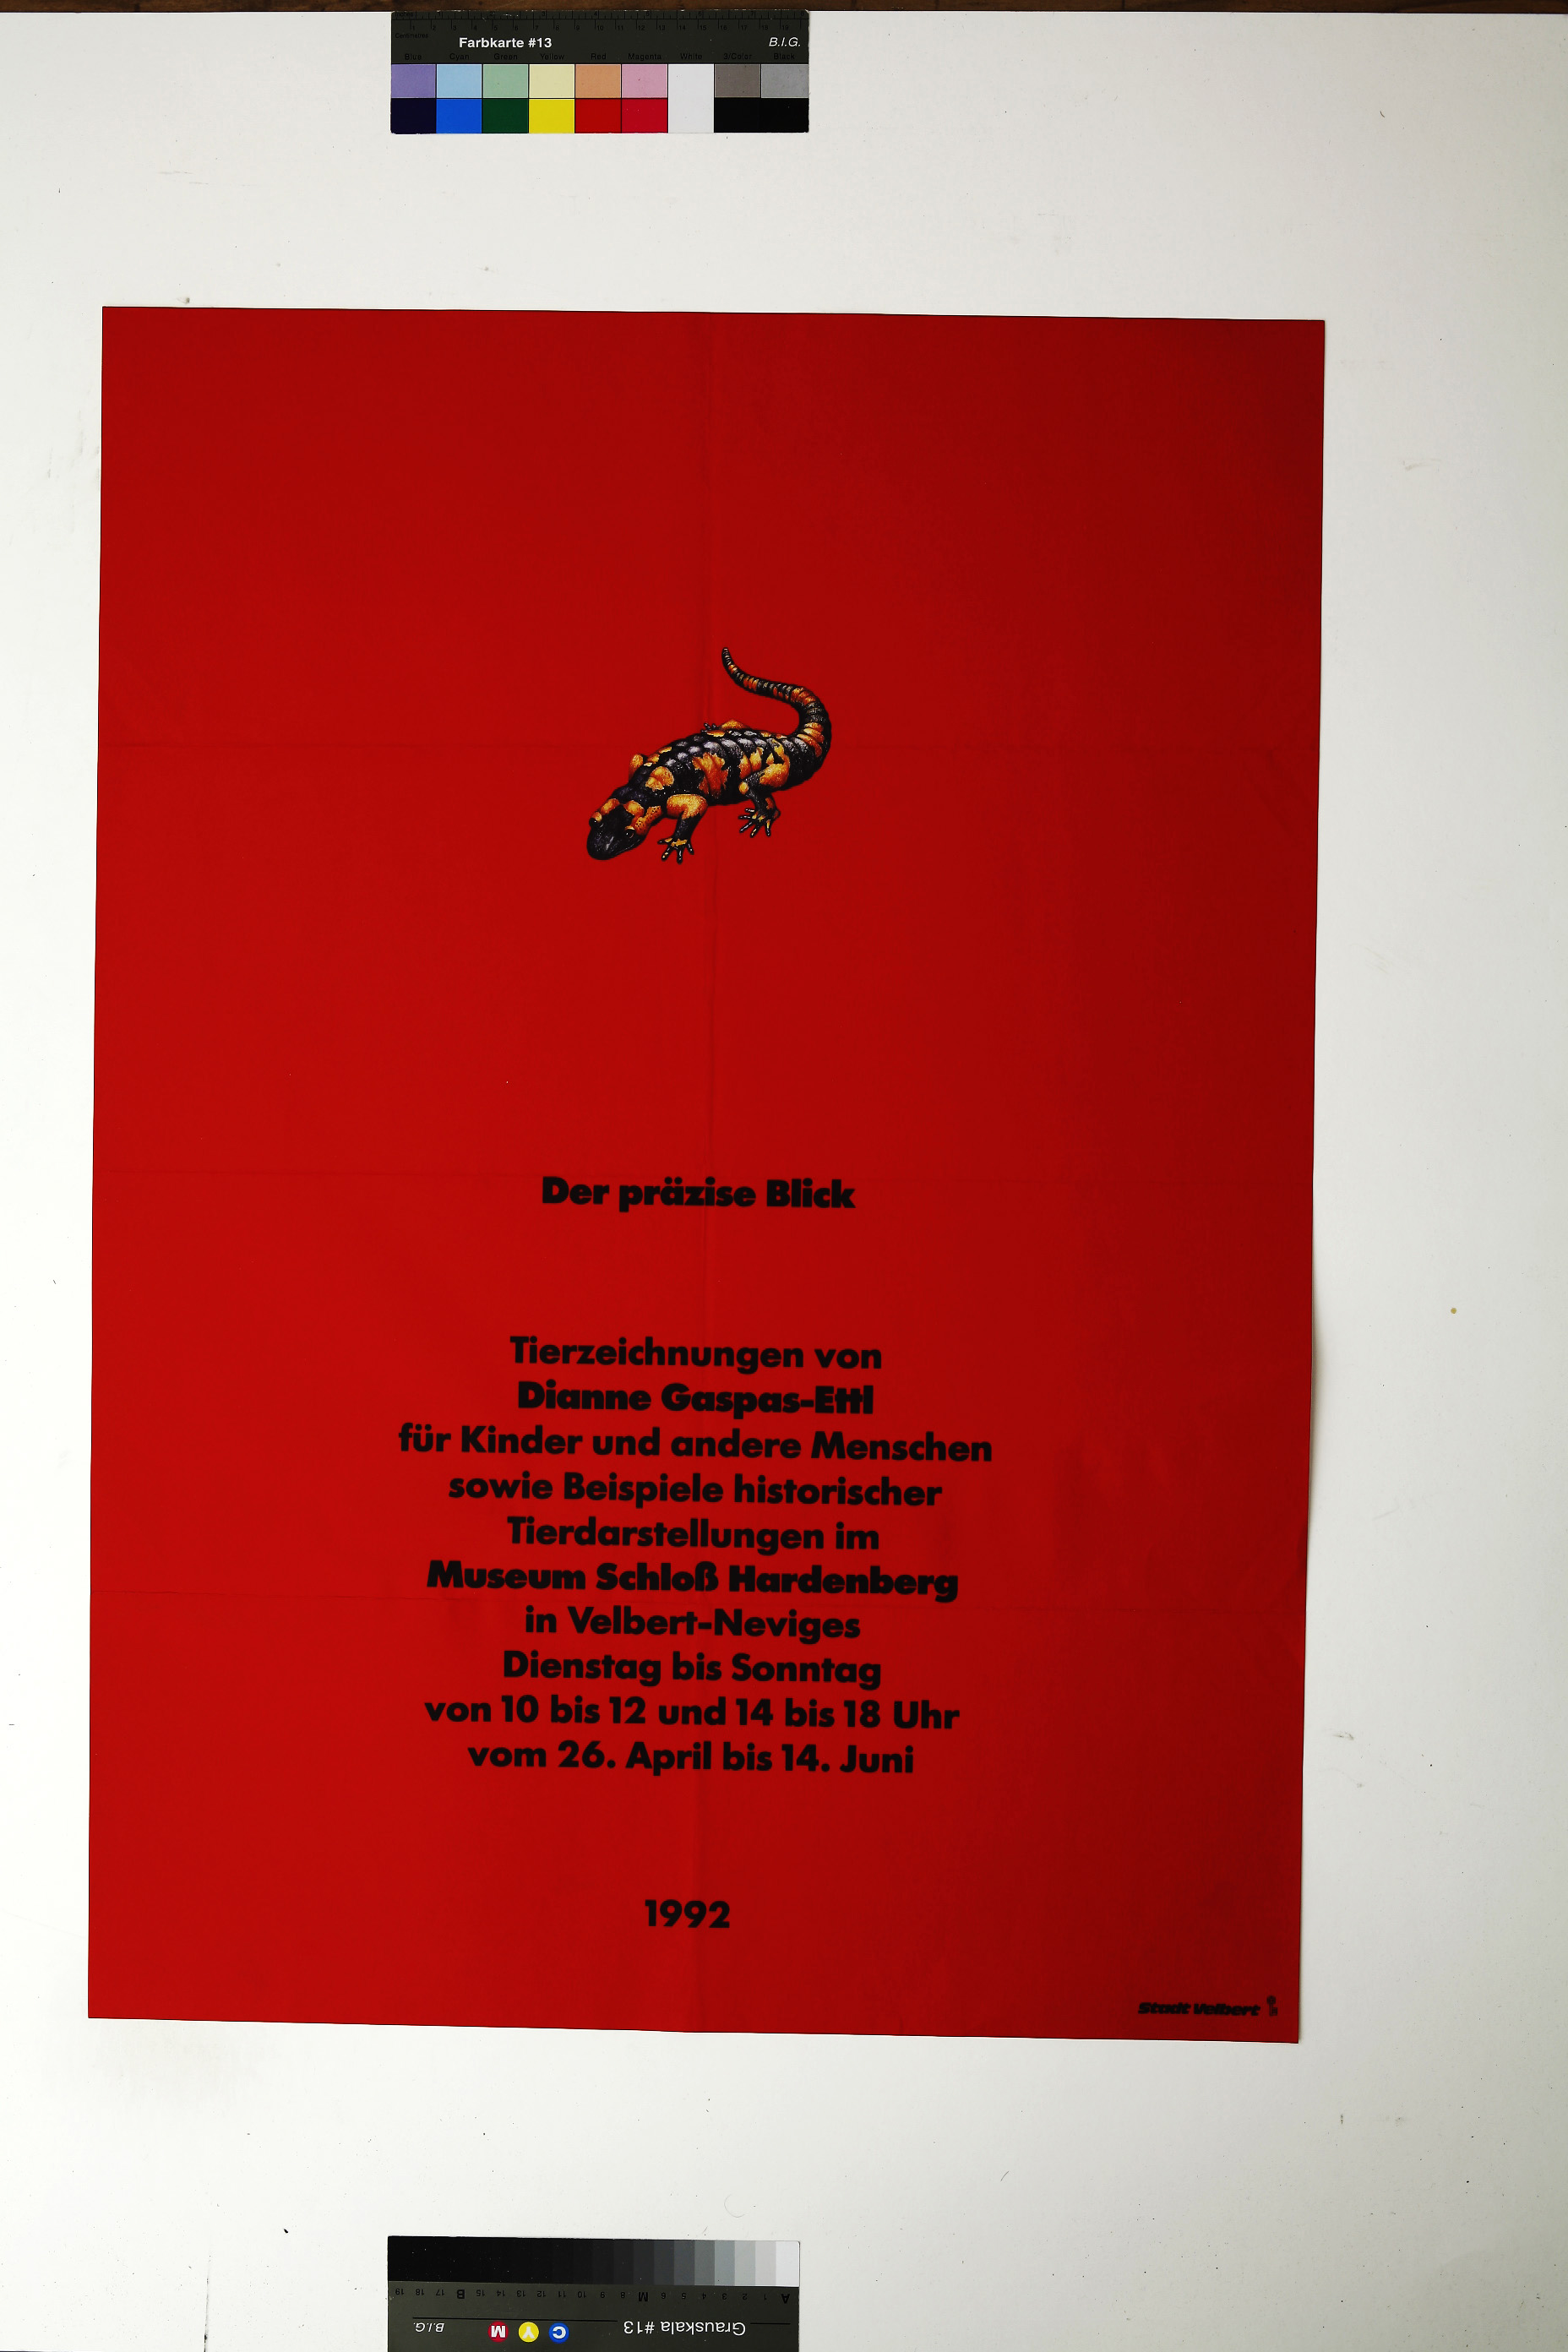
\includegraphics[width=\linewidth]{Abbildung_1_(acht1_028)}
\centering
\caption{Ausstellungsplakat – Tierzeichnungen von Dianne Gaspas-Ettl, Museum Schloß Hardenberg, 26.04.1992-14.06.1992 (acht1\_028).}
\end{figure}

\newpage
\begin{figure}[ht]
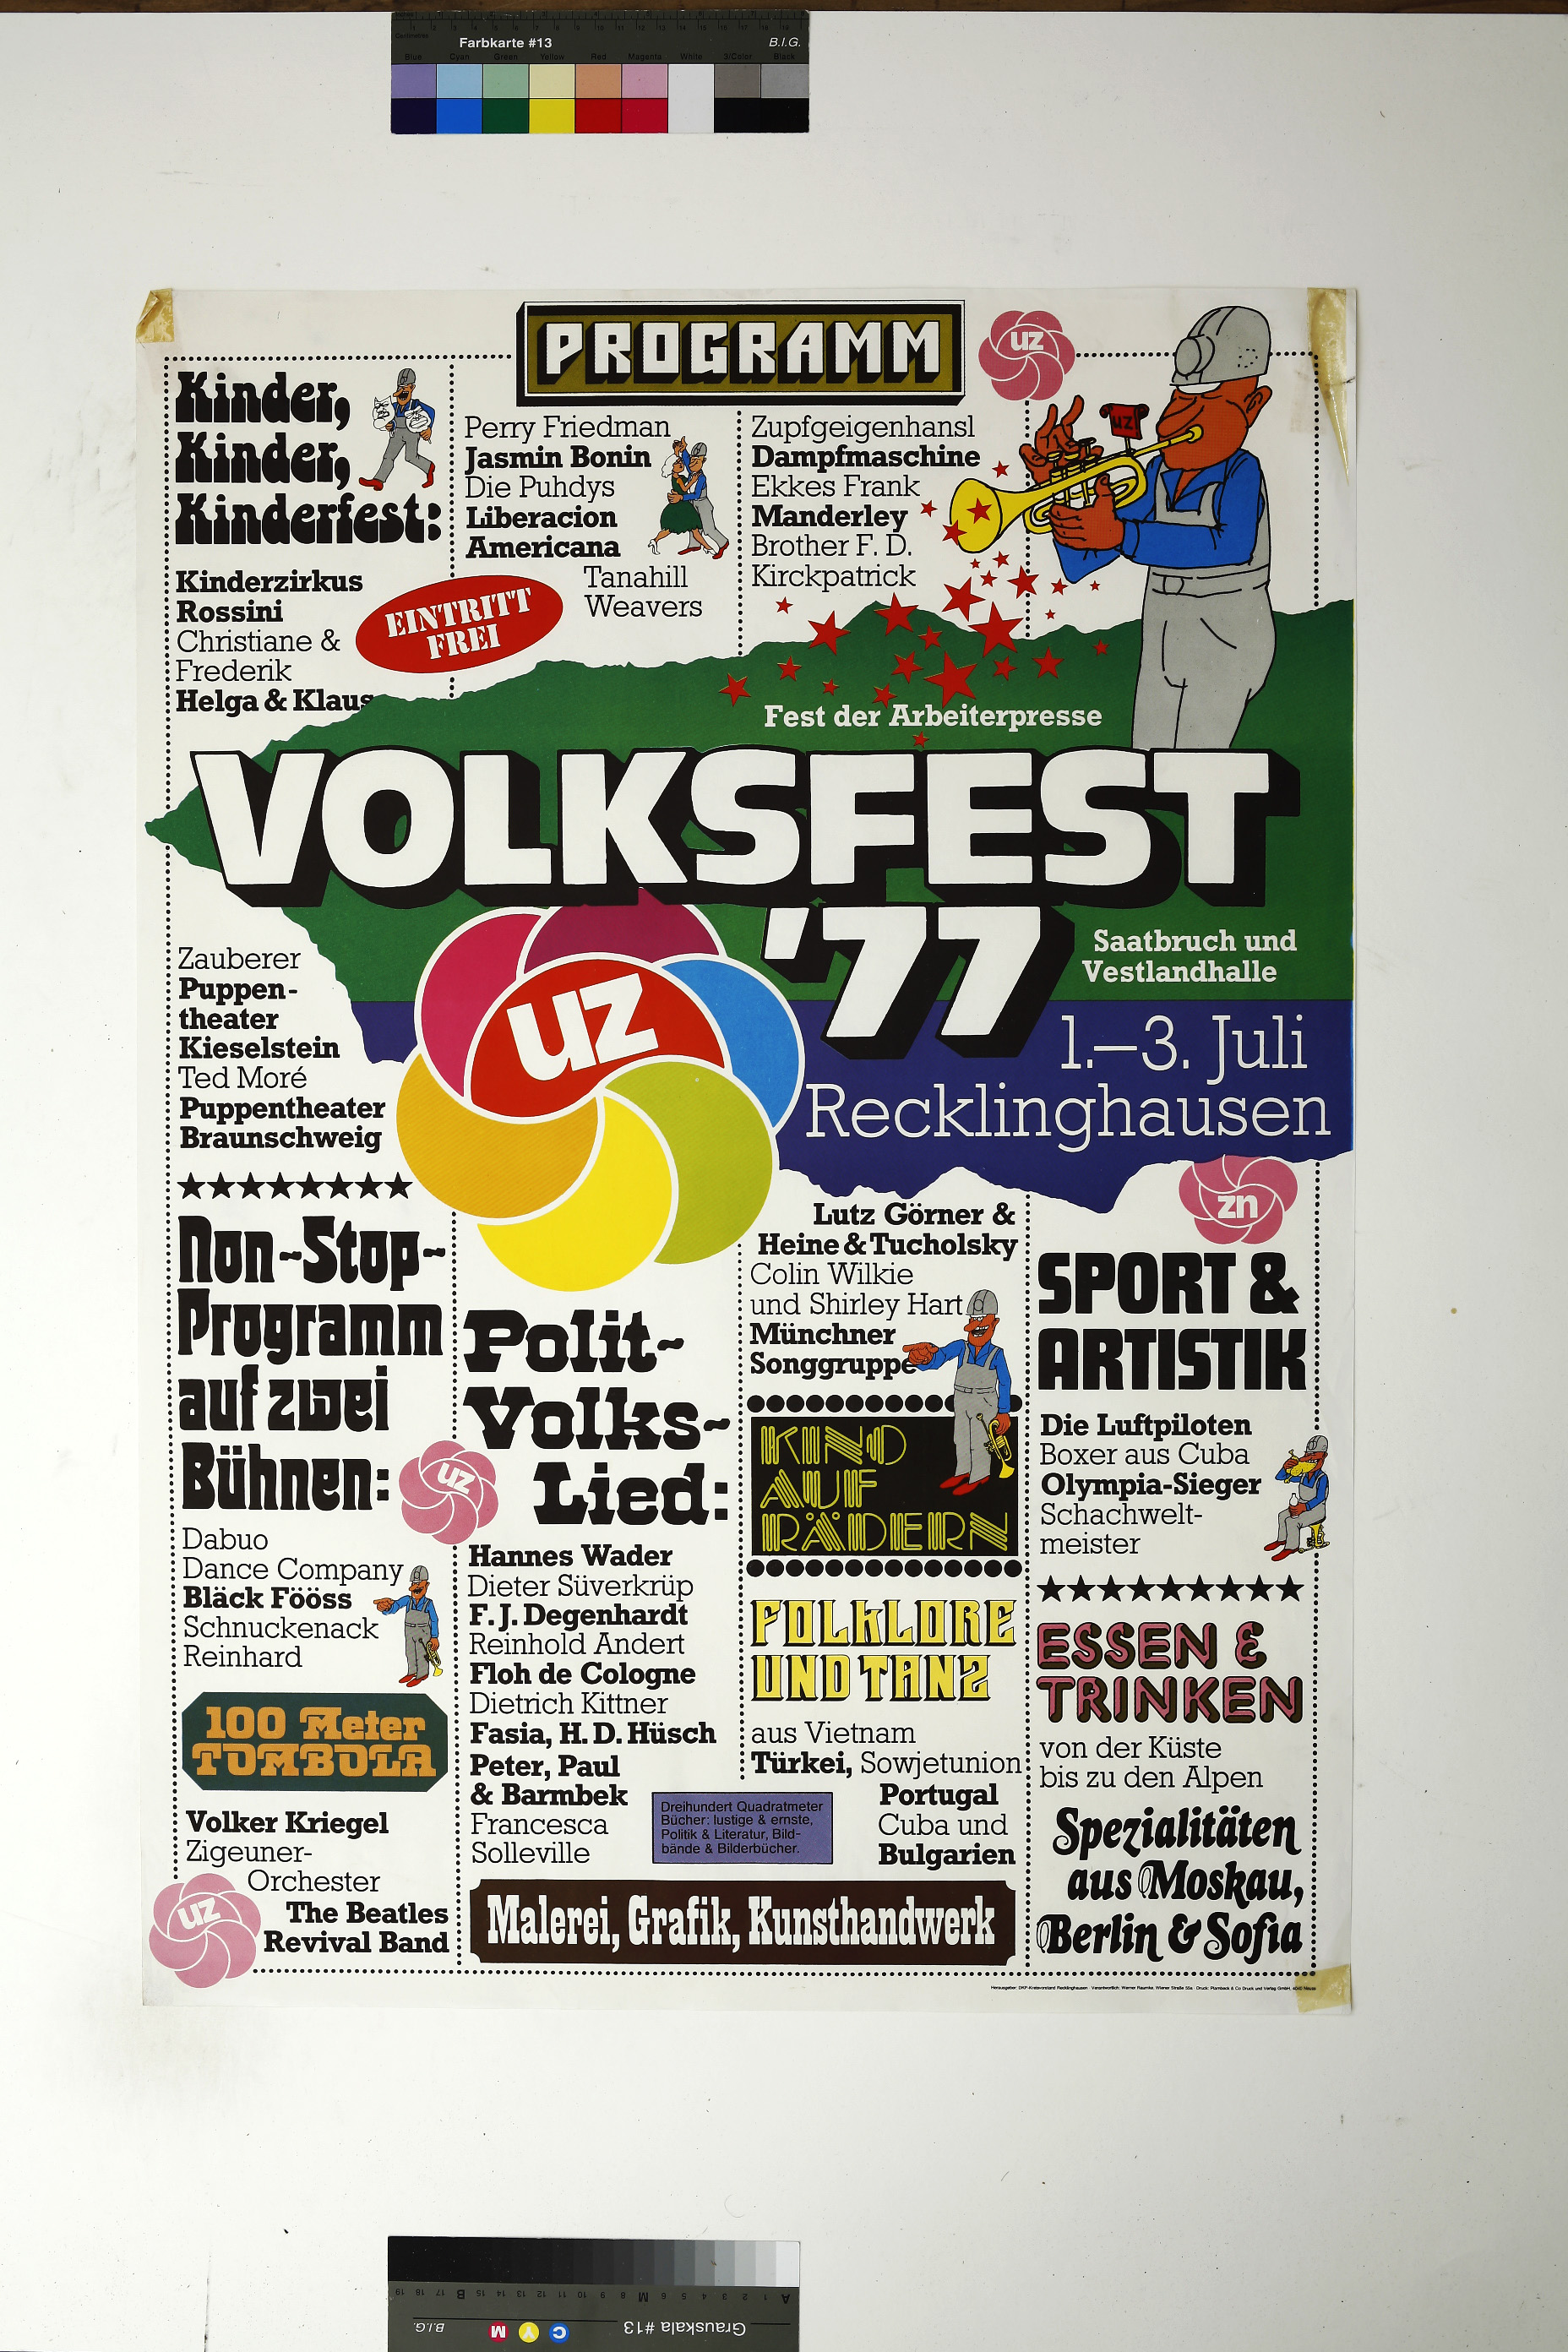
\includegraphics[width=\linewidth]{Abbildung_2_(acht1_066)}
\centering
\caption{Programmplakat – Volksfest ´77, UZ Recklinghausen, 1.07.1977-03.07.1977 (acht1\_066).}
\end{figure}

\newpage
\begin{figure}[ht]
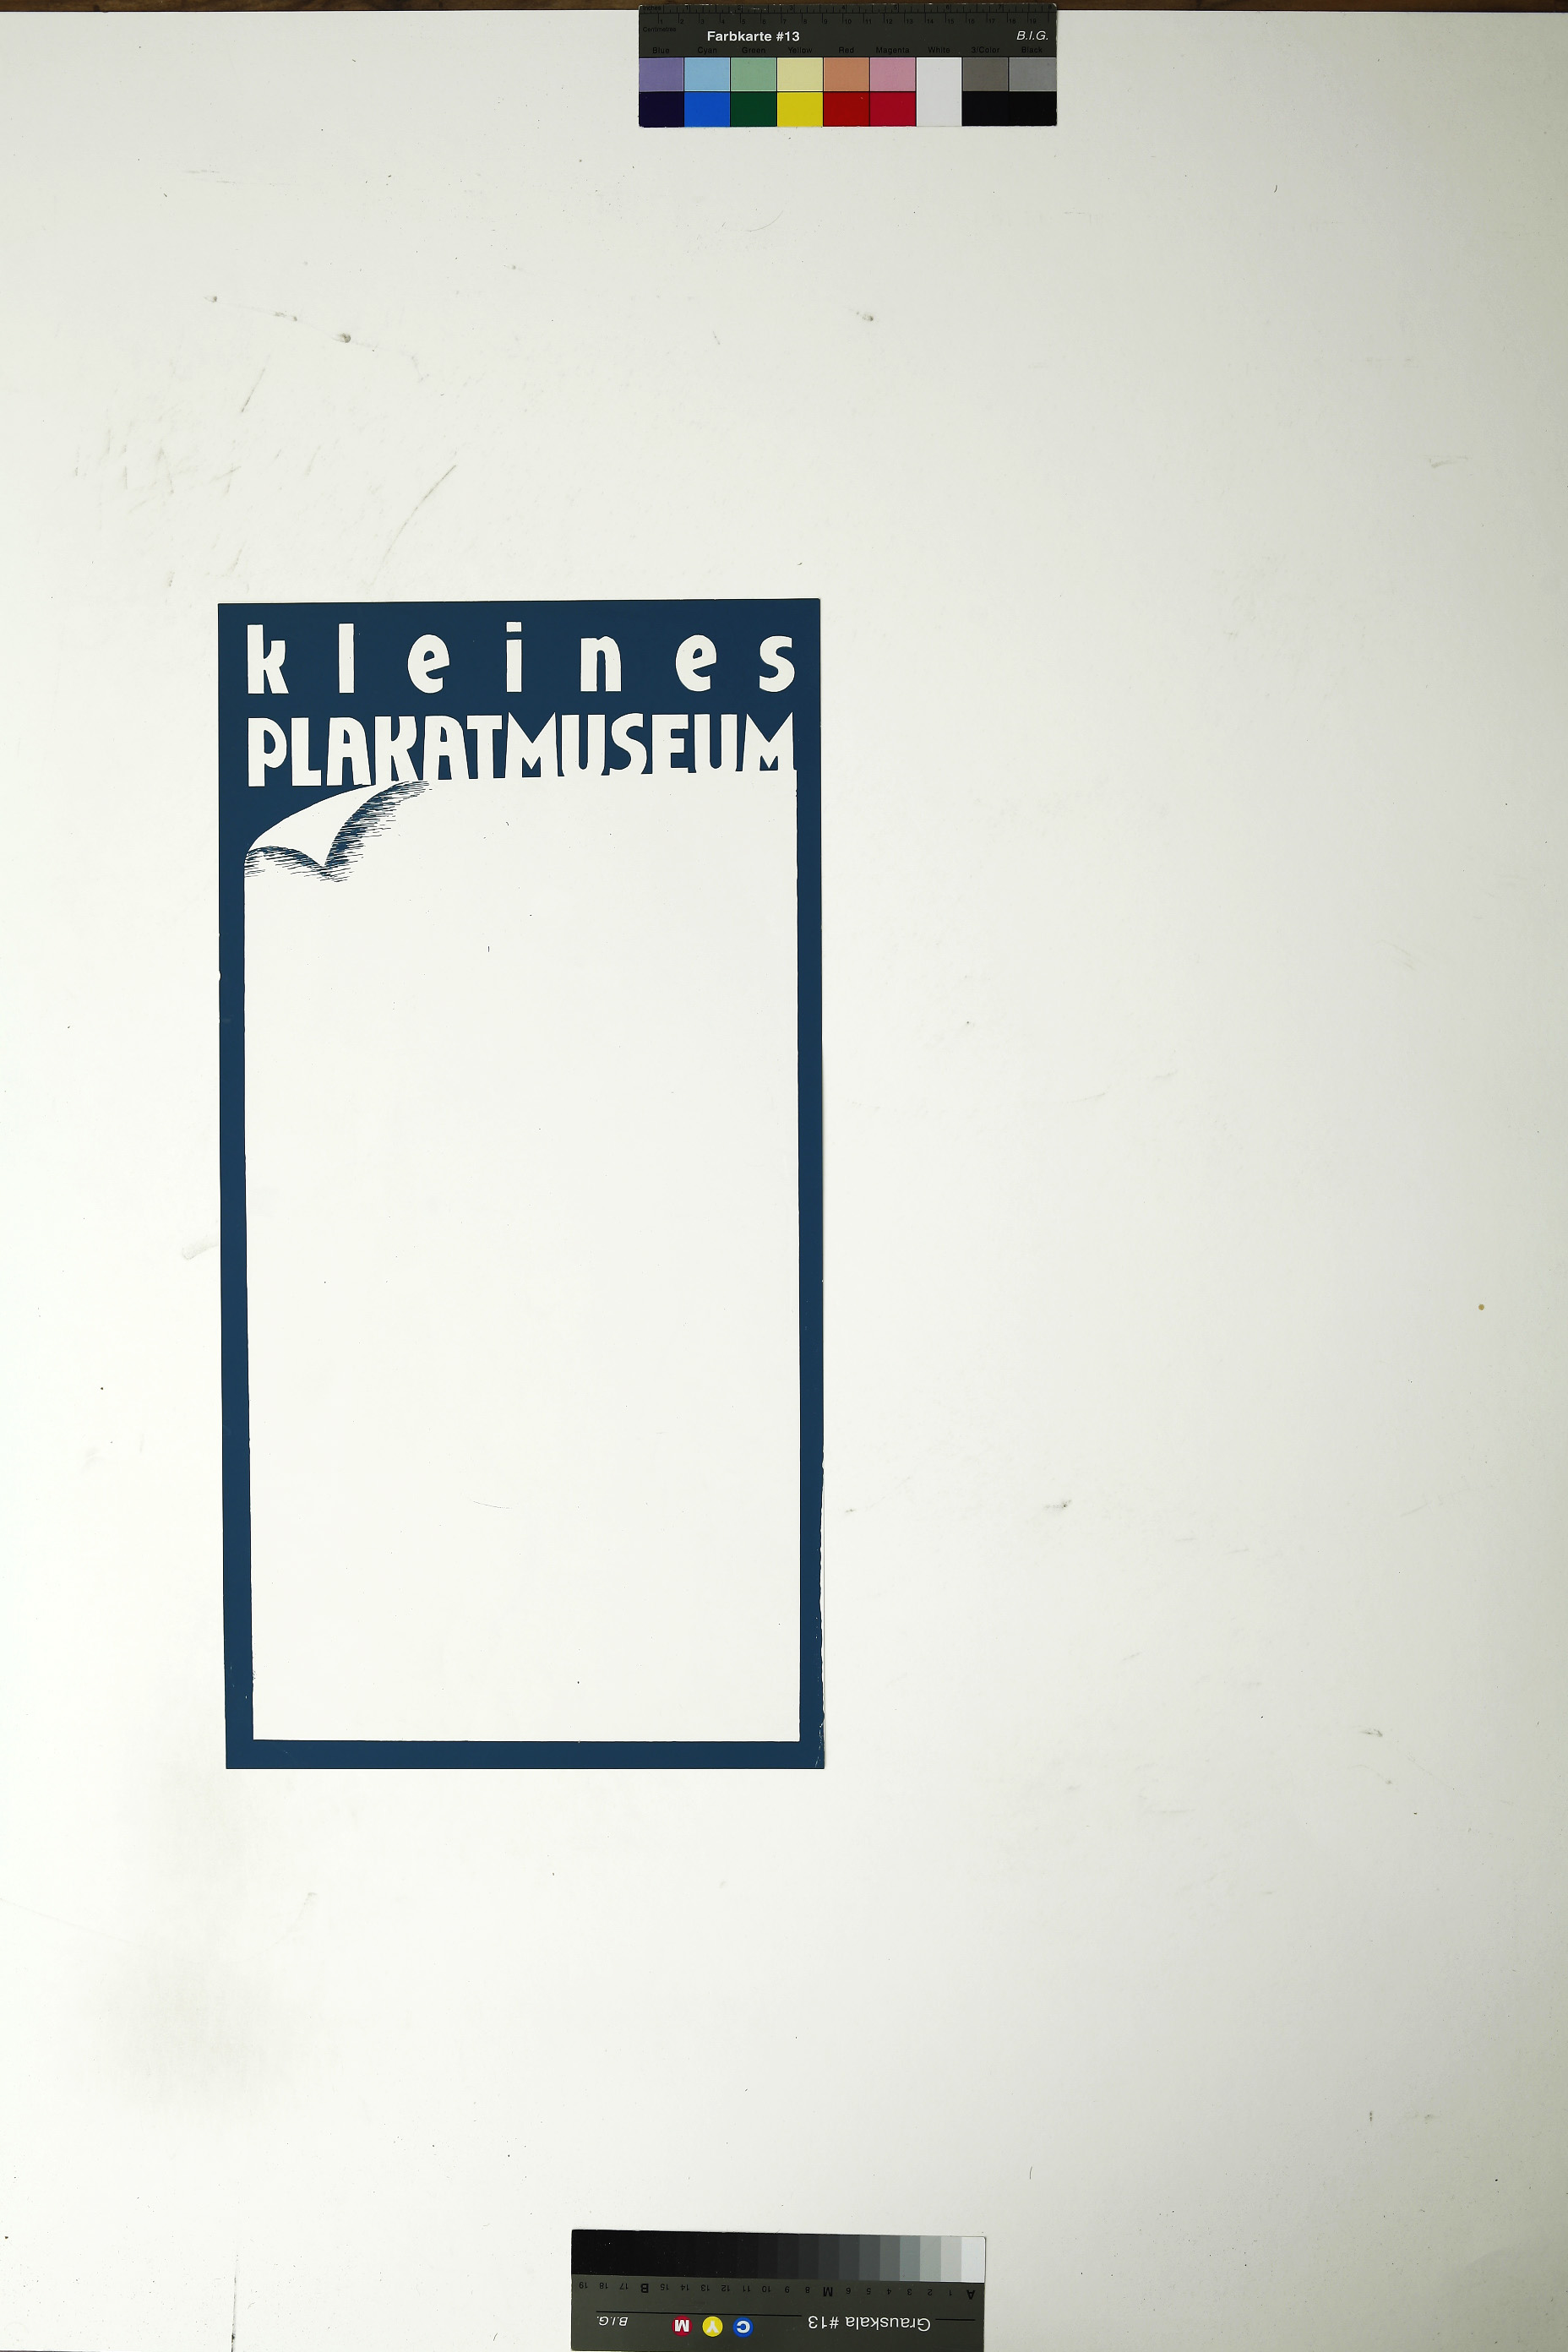
\includegraphics[width=\linewidth]{Abbildung_3_(acht2_043)}
\centering
\caption{Eindruckplakat – Kleines Plakatmuseum, ohne Datum (acht2\_043).}
\end{figure}

\newpage
\begin{landscape}
\begin{figure}[ht]
	\begin{subfigure}[b]{0.5\linewidth}
	\centering
	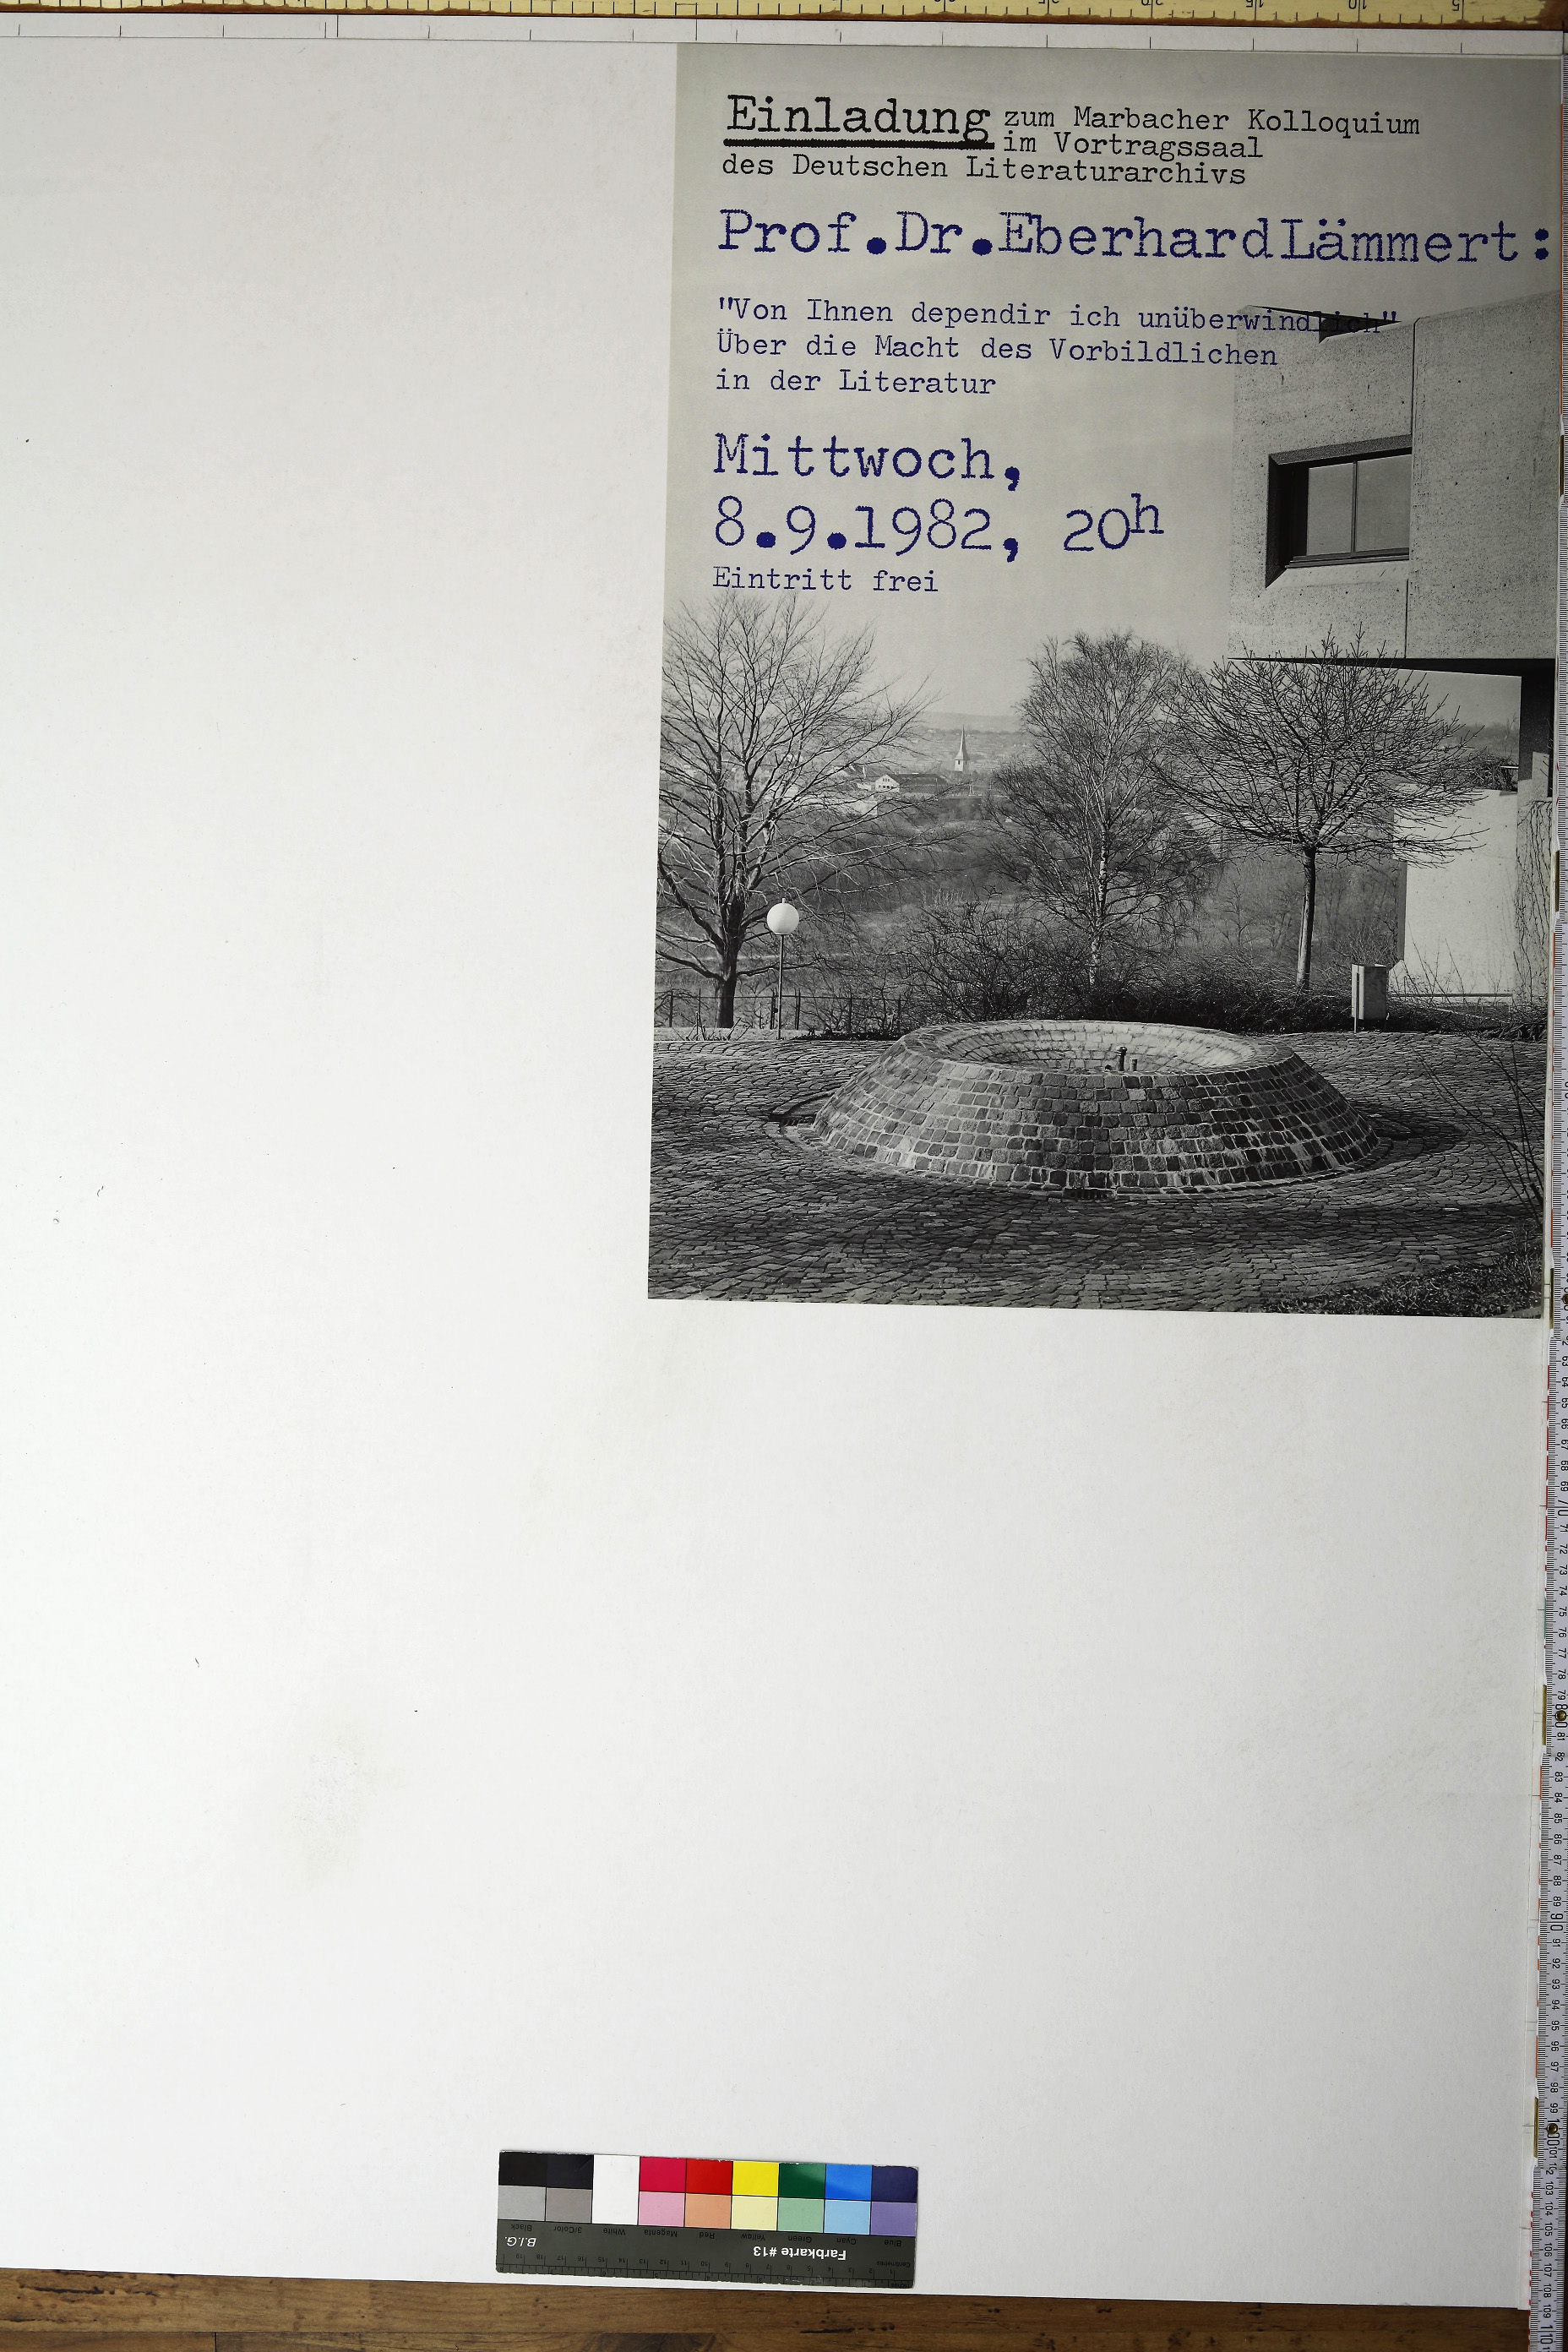
\includegraphics[height=\linewidth]{Abbildung_4a_(acht3_212)}
	\end{subfigure}
	\begin{subfigure}[b]{0.5\linewidth}
	\centering
	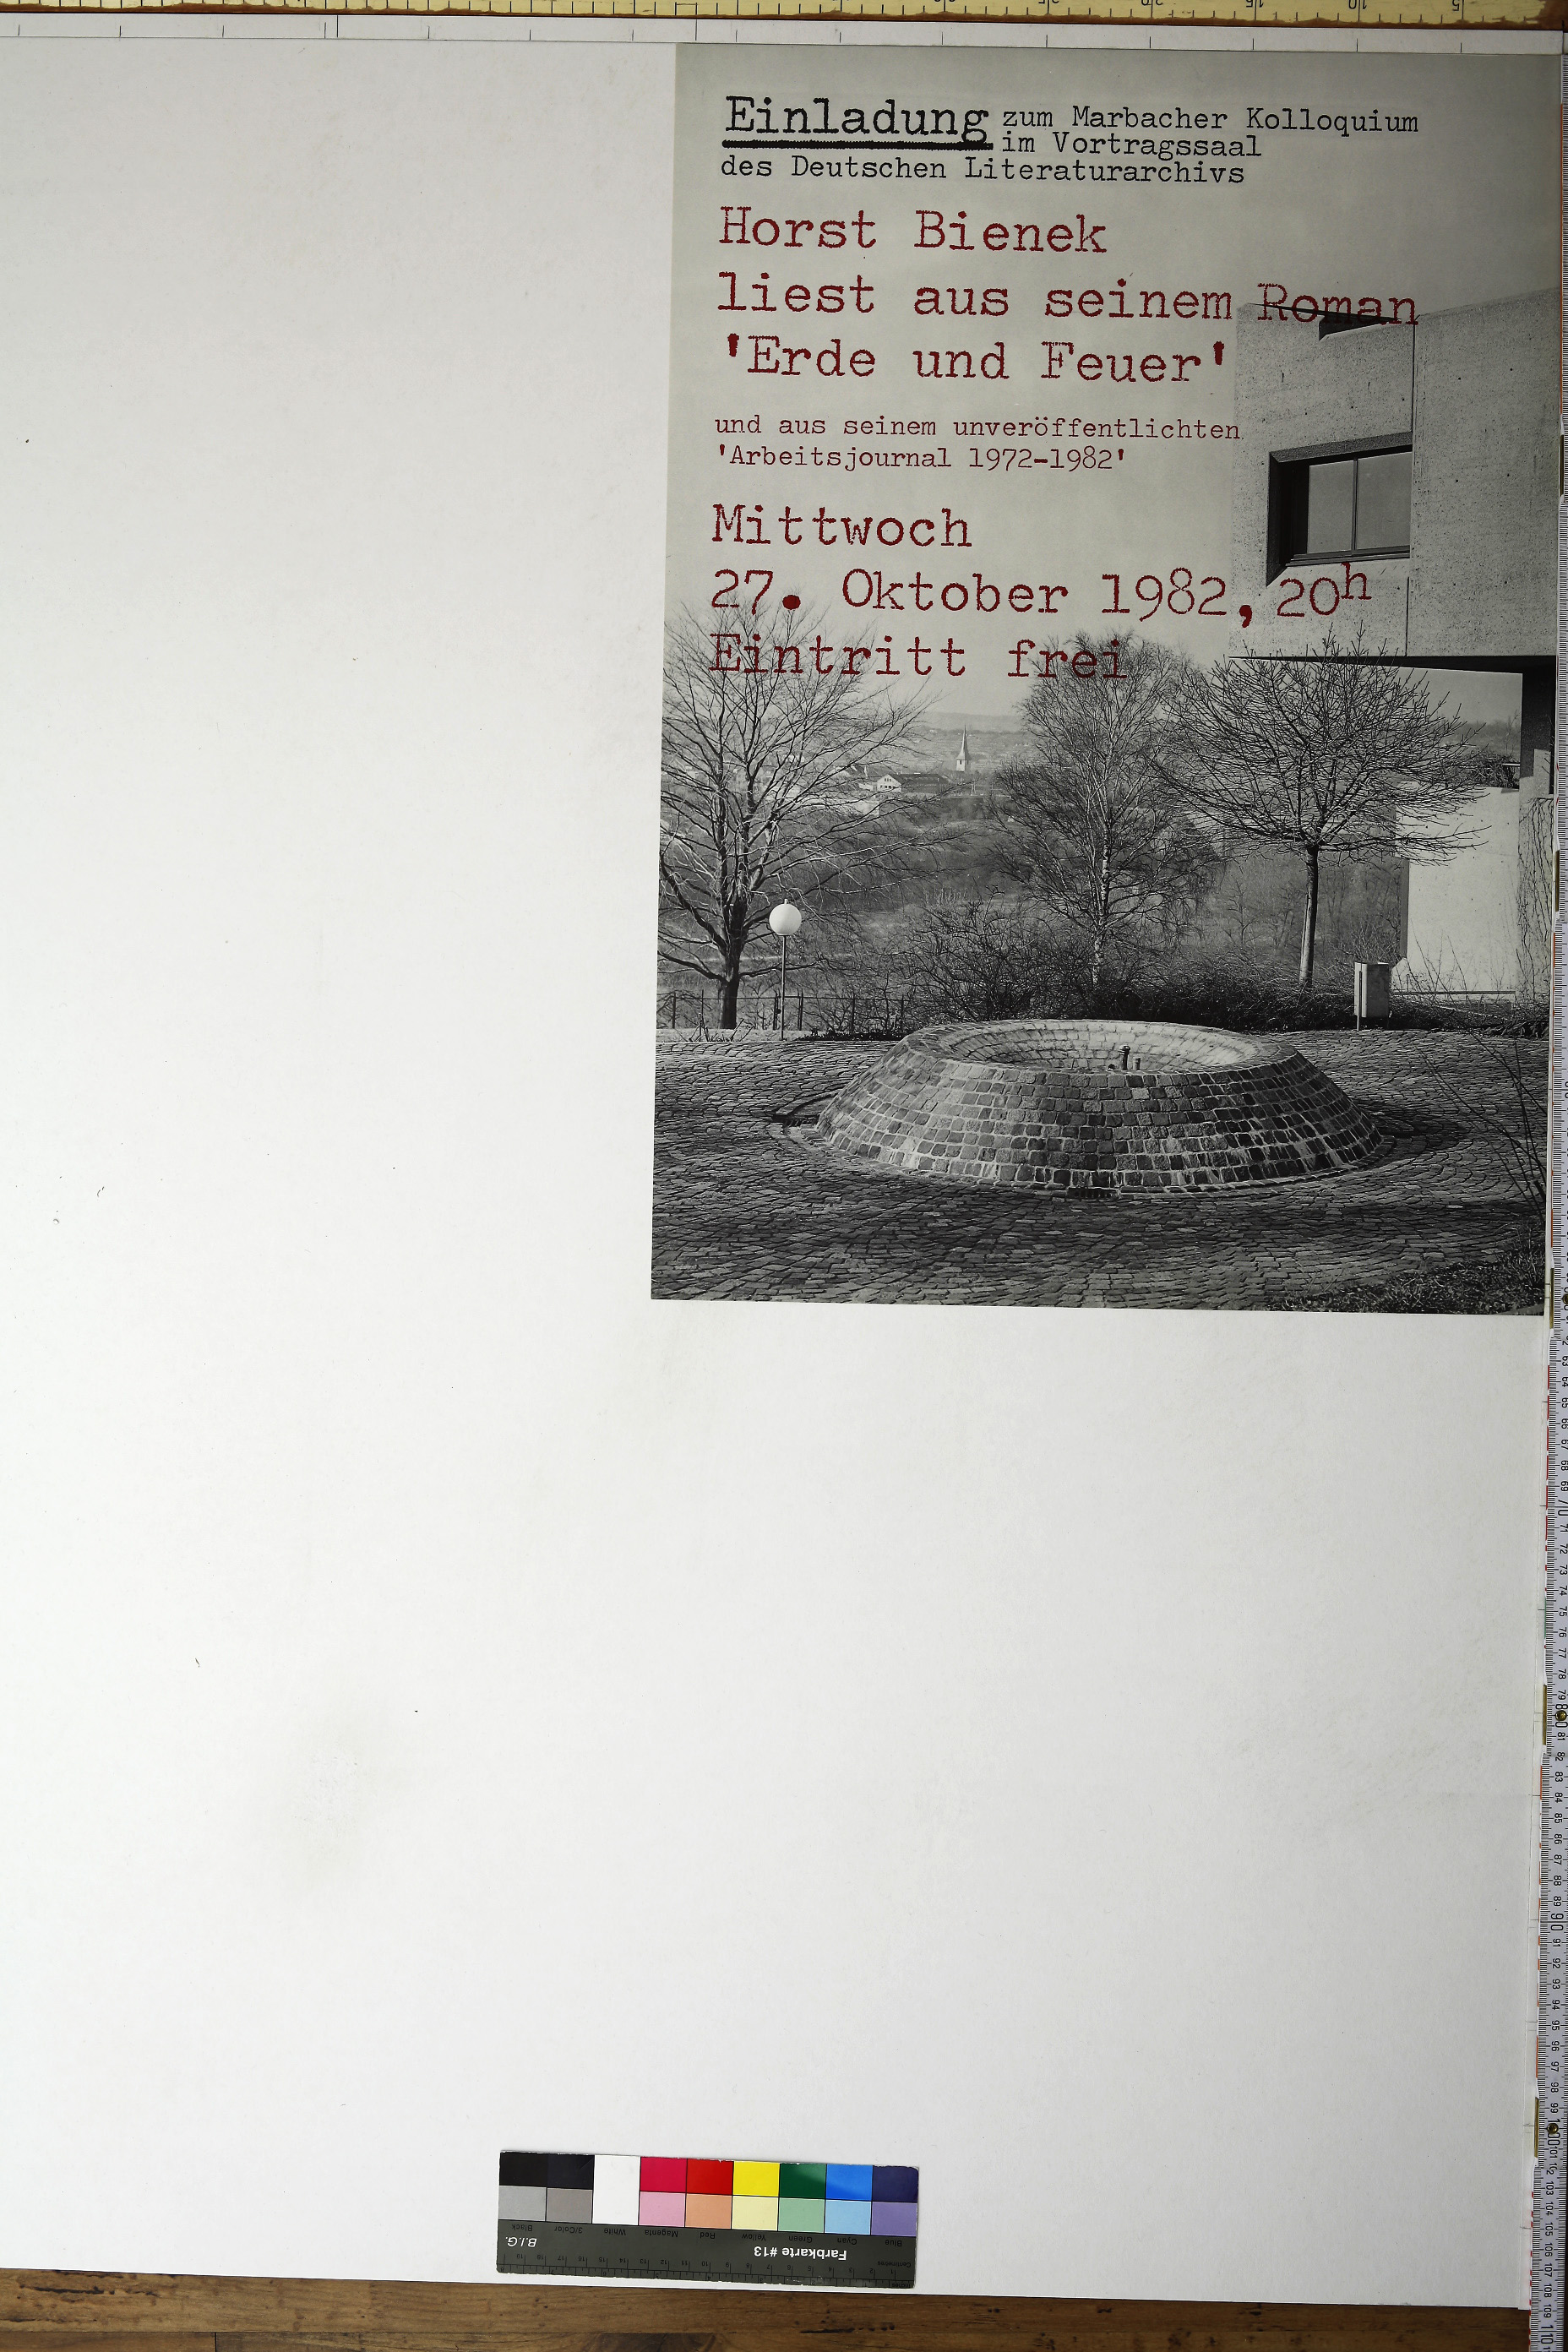
\includegraphics[height=\linewidth]{Abbildung_4b_(acht3_213)}
	\end{subfigure}
	\caption{Eindruckplakate – Prof. Dr. Eberhardt Lämmert: „Von Ihnen dependir ich unüberwindlich“ Über die Macht des Vorbildlichen in der Literatur, Marbacher Kolloquium, 08.09.1982 (acht3\_212); Horst Bienek liest aus seinem Roman „Erde und Feuer“, Marbacher Kolloquium, 27.10.1982 (acht3\_213).}
\end{figure}
\end{landscape}

\newpage
\begin{figure}[ht]
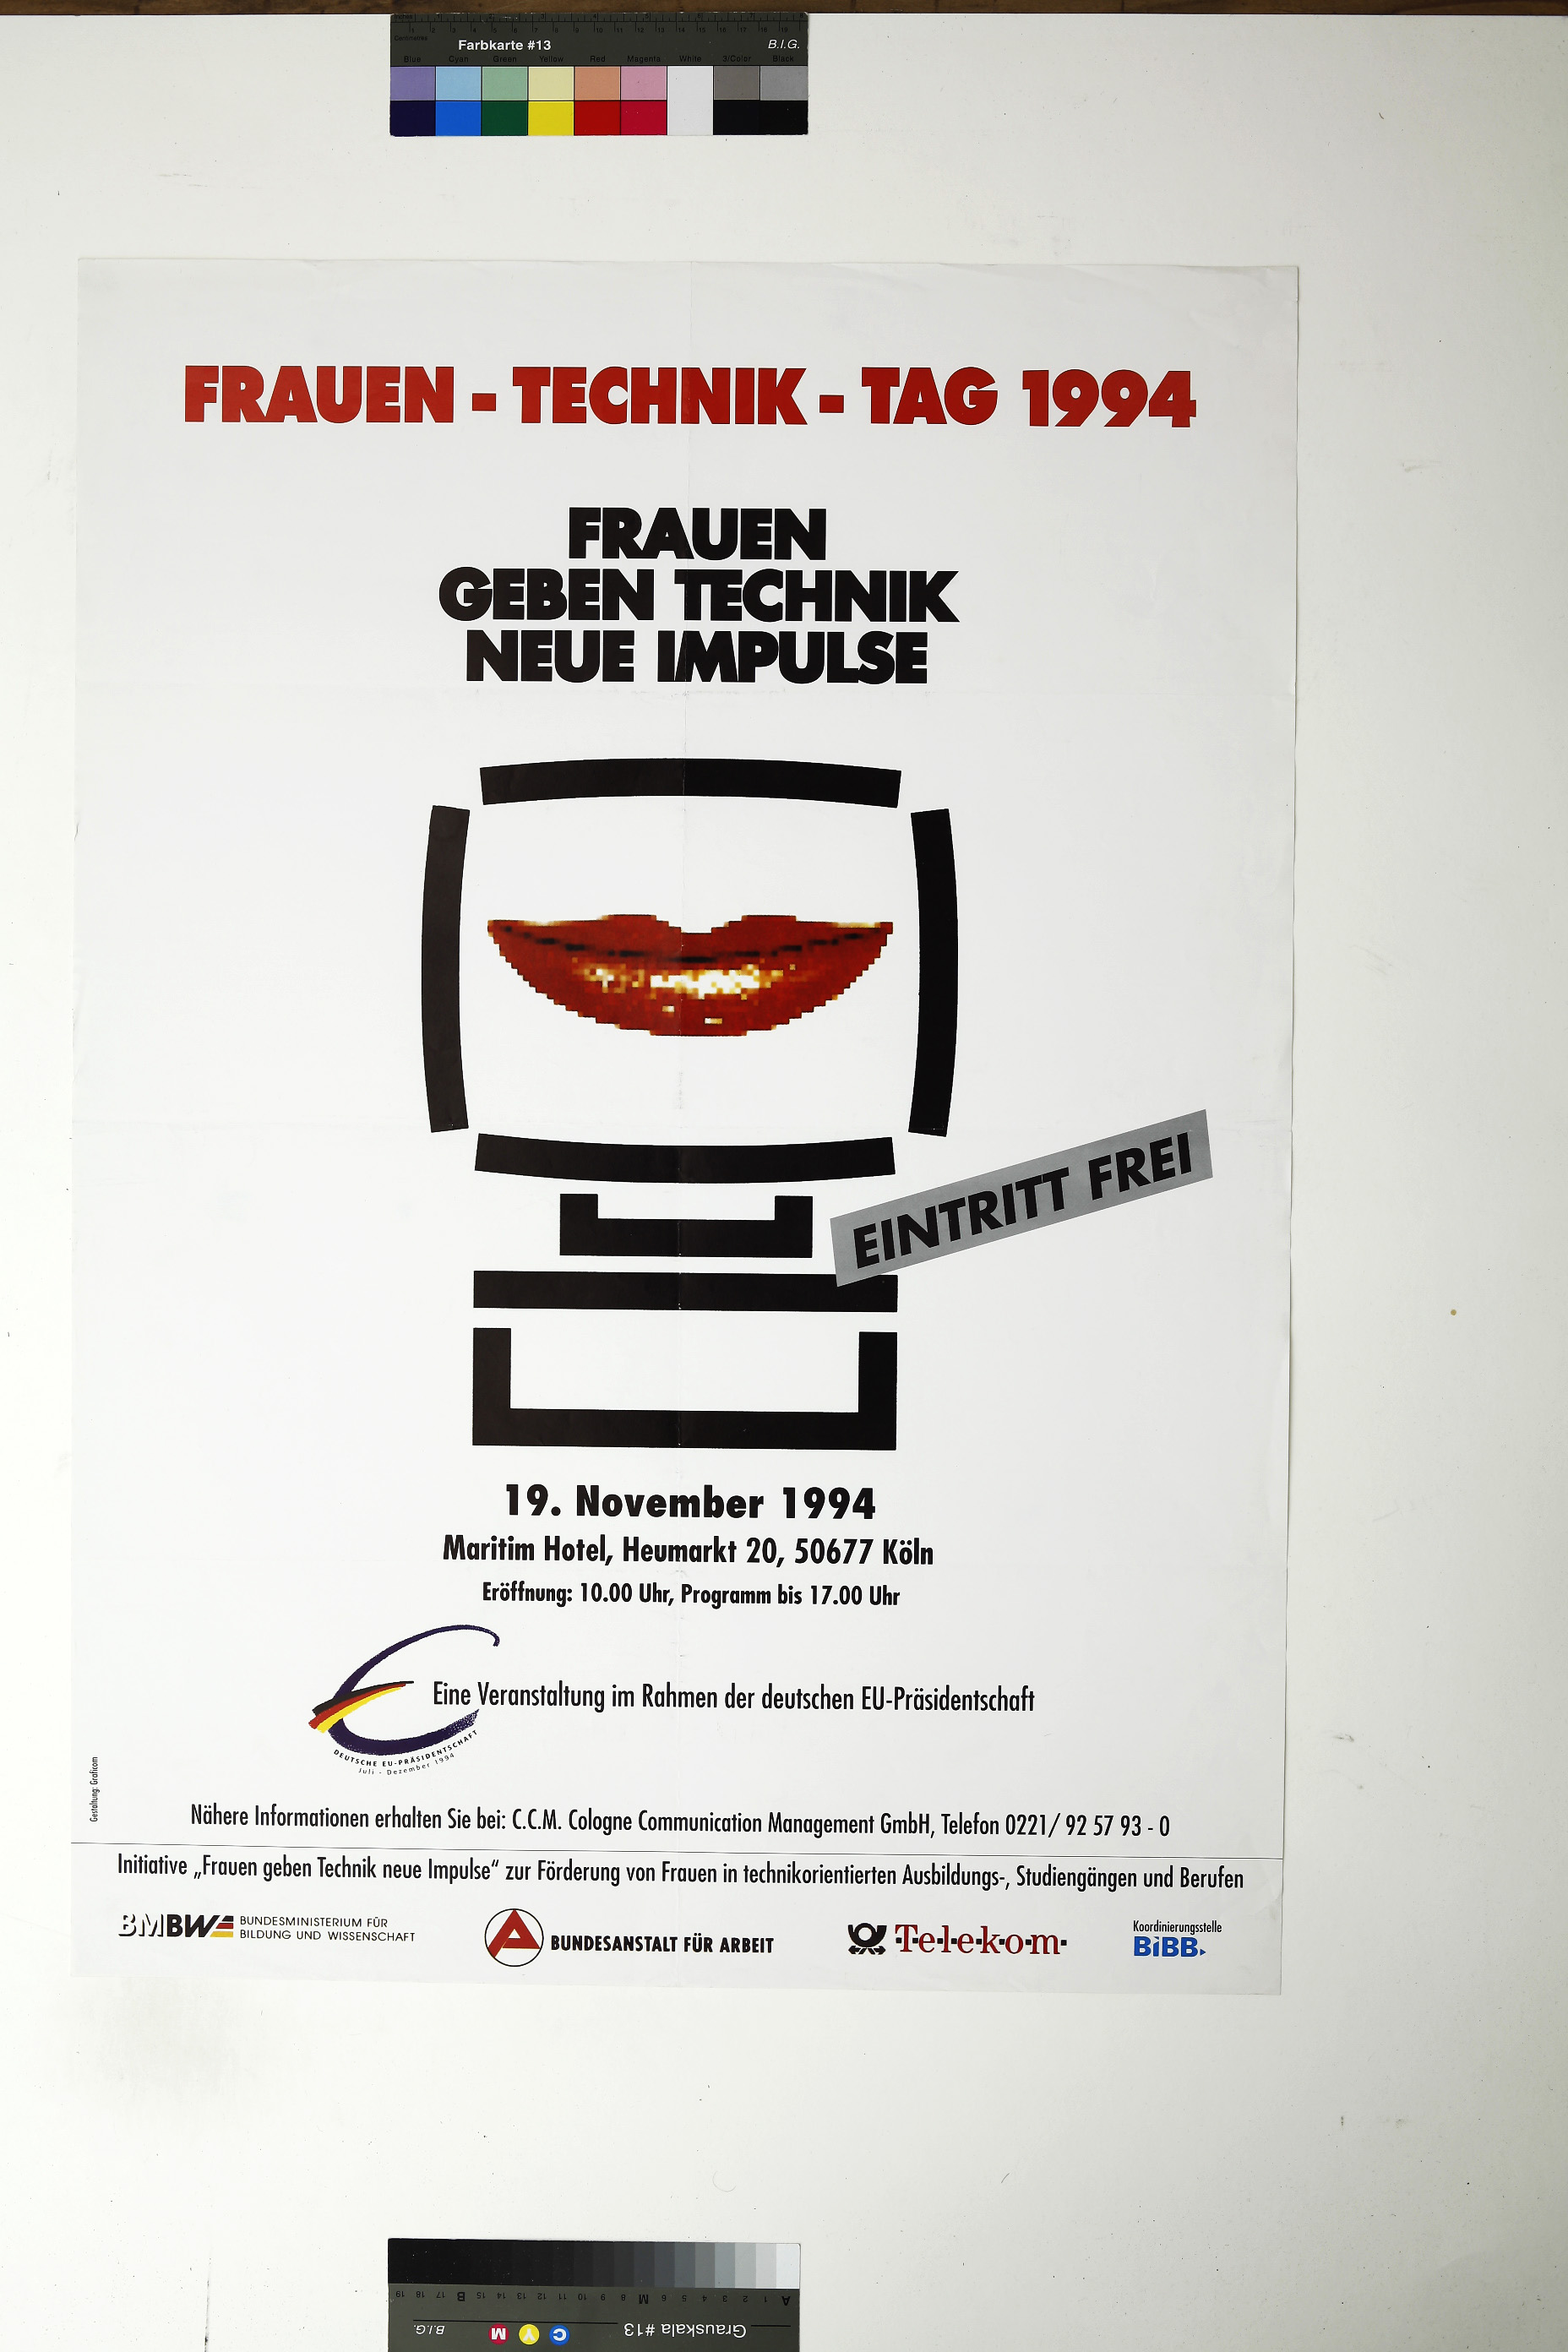
\includegraphics[width=\linewidth]{Abbildung_5_(acht2_189)}
\centering
\caption{Veranstaltungsplakat – Frauen – Technik – Tag 1994, Initiative „Frauen geben Technik neue Impulse“ zur Förderung von Frauen in technikorientierten Ausbildungs-, Studiengängen und Berufen, 19.11.1994 (acht2\_189).}
\end{figure}

\newpage
\begin{figure}[ht]
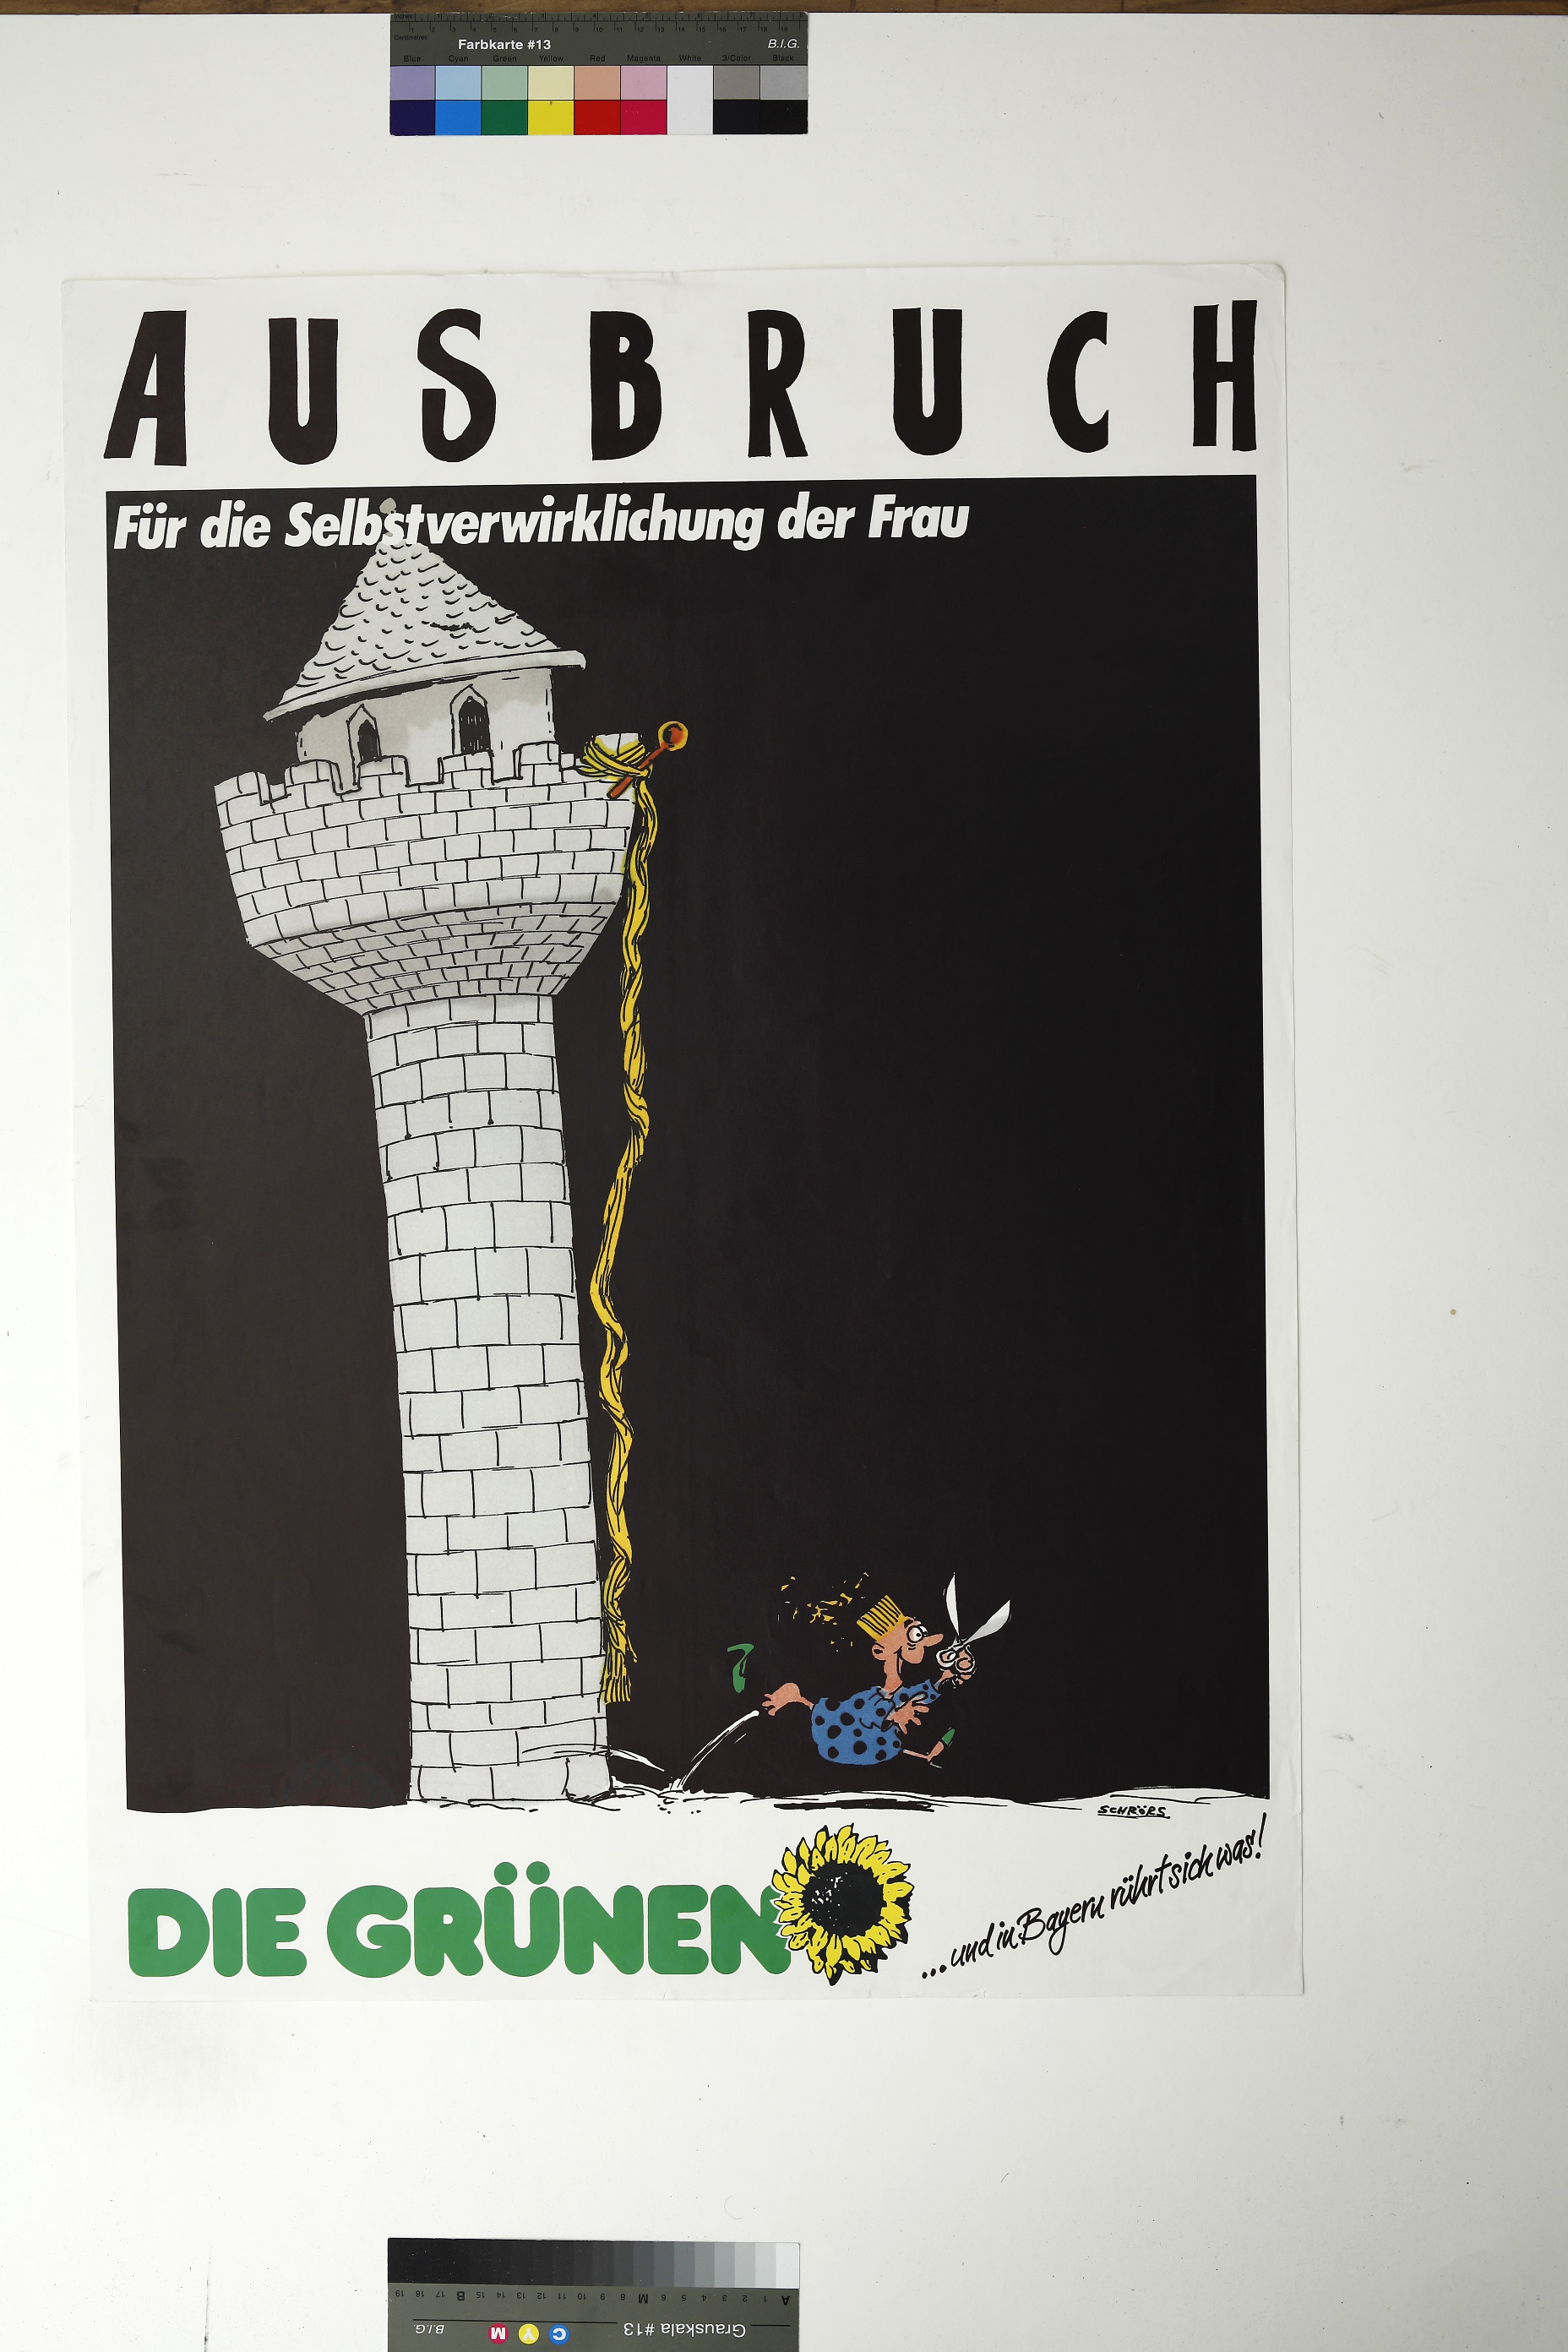
\includegraphics[width=\linewidth]{Abbildung_6_(acht2_208)}
\centering
\caption{Politisches Plakat – Ausbruch. Für die Selbstverwirklichung der Frau, Die Grünen, ohne Datum (acht2\_208).}
\end{figure}

\newpage
\begin{figure}[ht]
\includegraphics[width=\linewidth]{Abbildung_7_(fünfzehn5_070)}
\centering
\caption{Politisches Plakat - Todesstrafe in den USA Abschaffen!, amnesty international, ohne Datum (fünfzehn5\_070).}
\end{figure}

\newpage
\begin{figure}[ht]
	\begin{subfigure}[b]{0.5\linewidth}
	\centering
	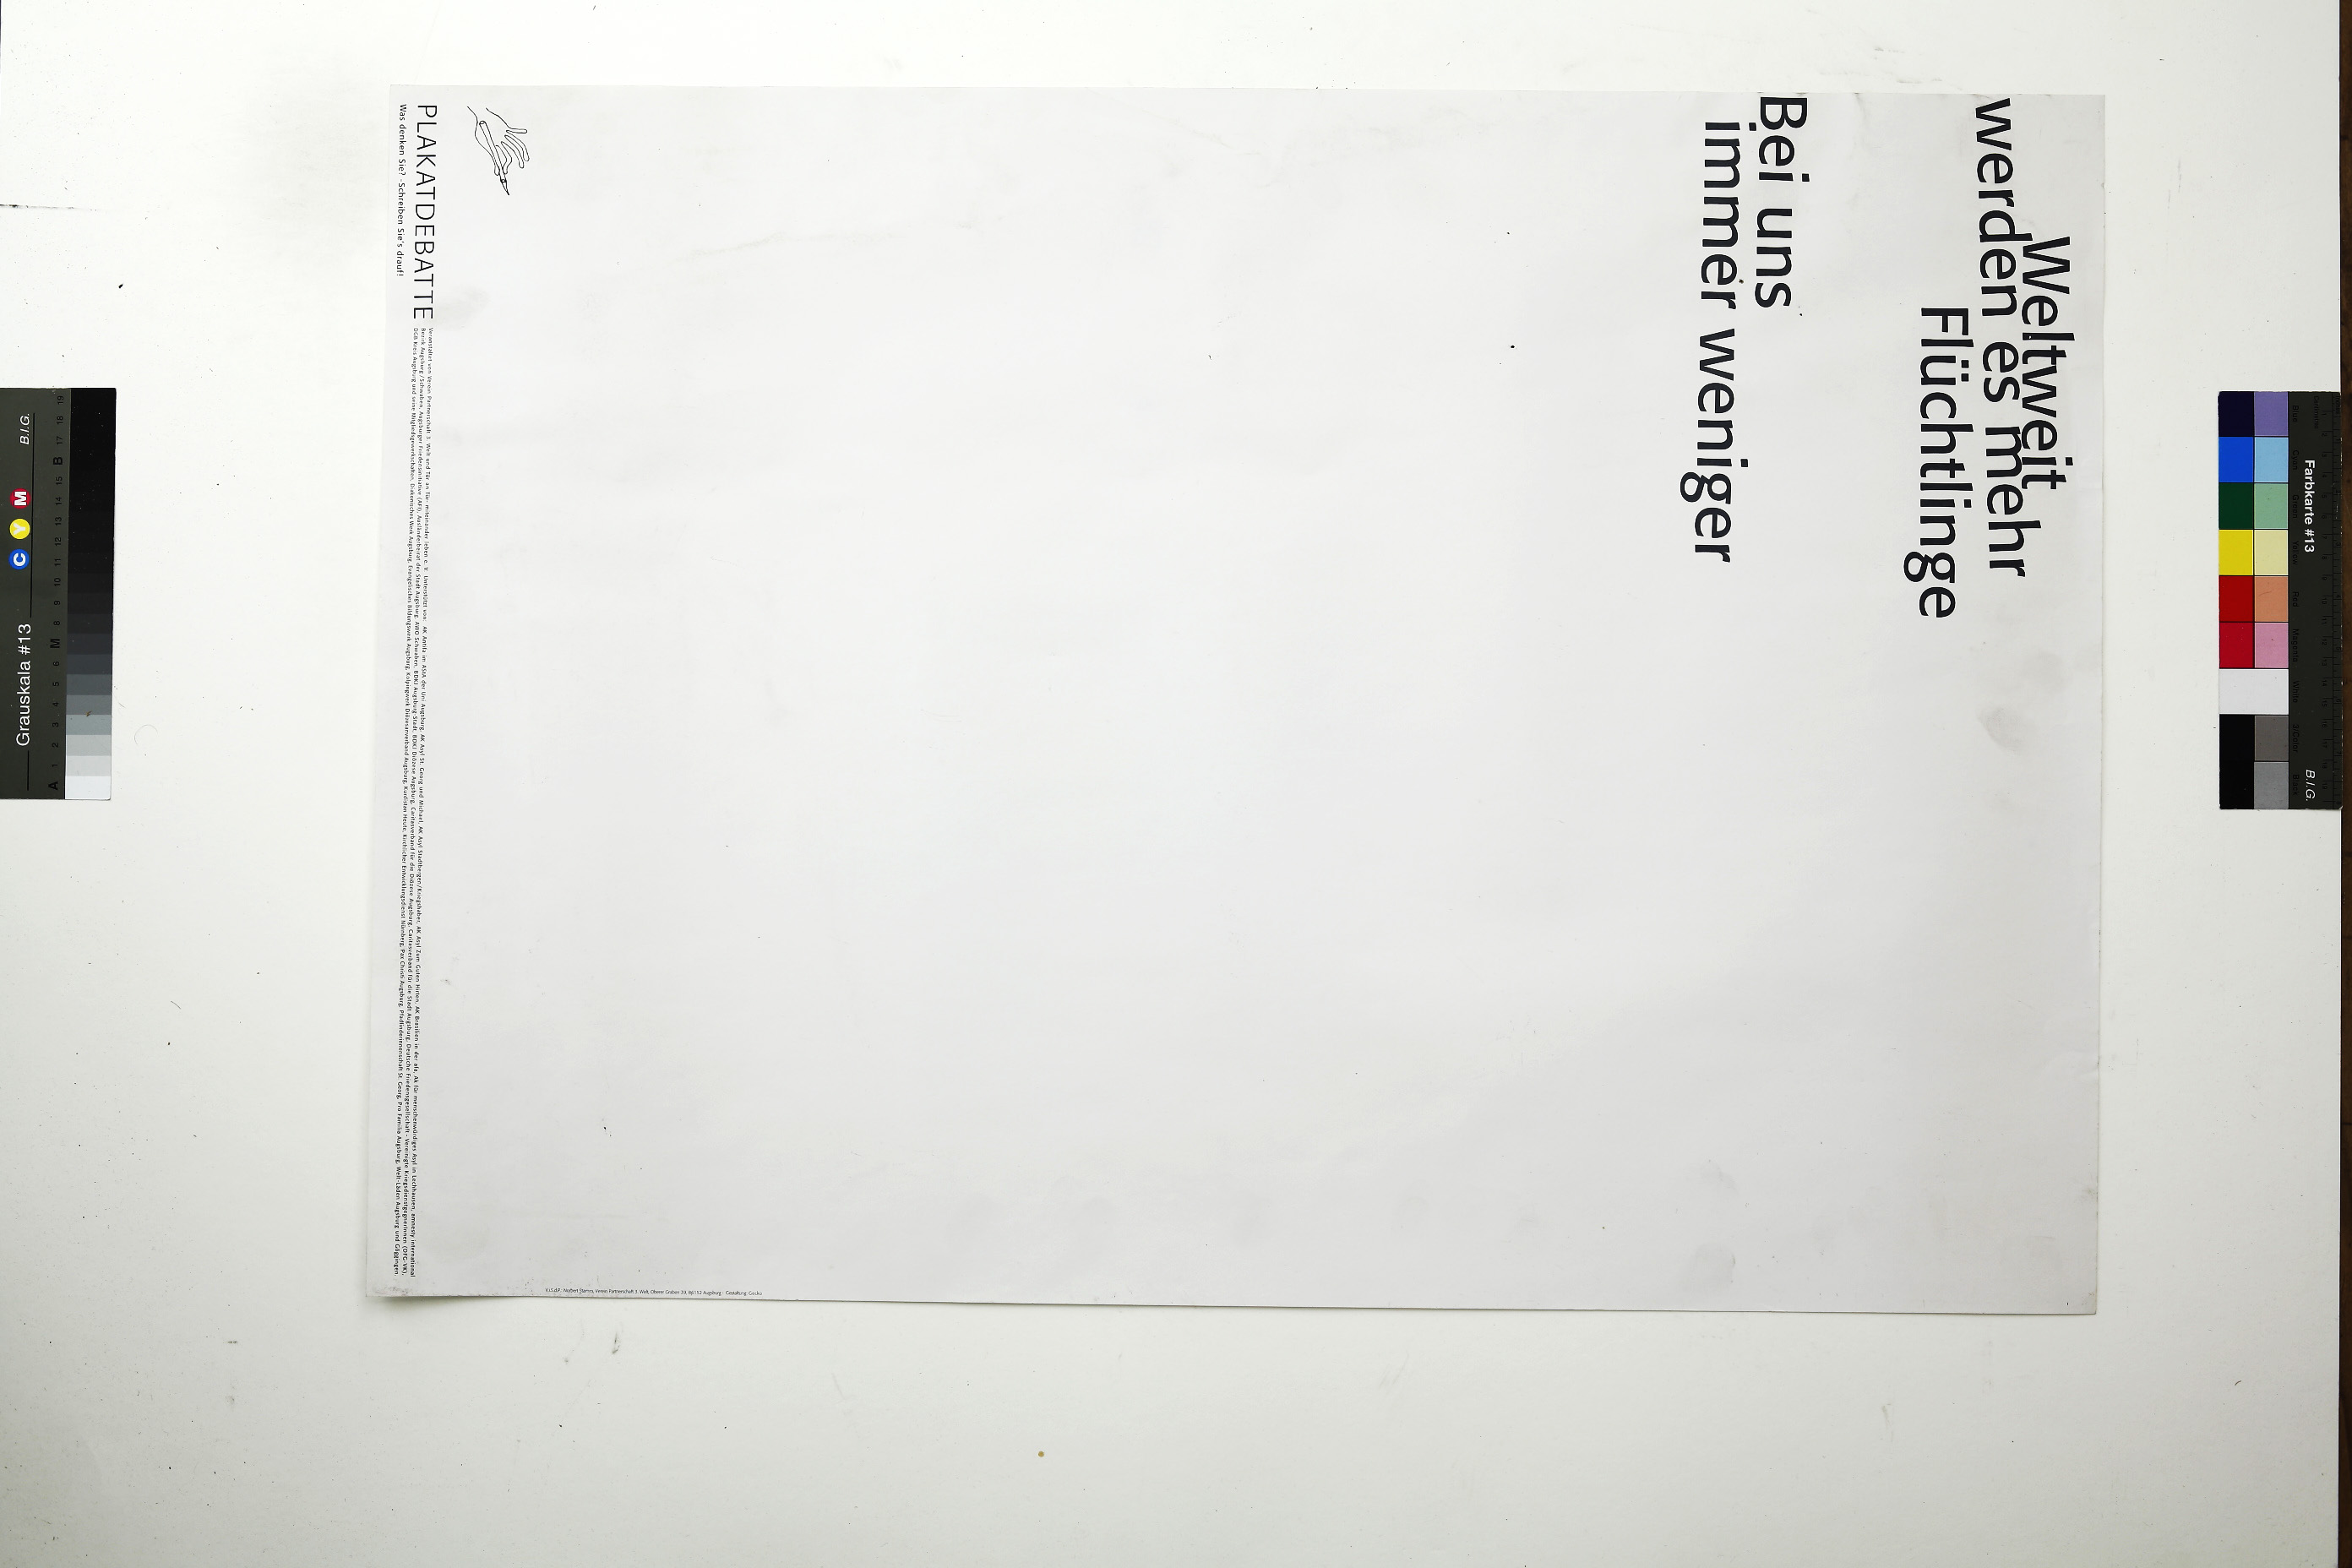
\includegraphics[height=\linewidth, angle=90]{Abbildung_8a_(acht1_079)}
	\end{subfigure}
	\begin{subfigure}[b]{0.5\linewidth}
	\centering
	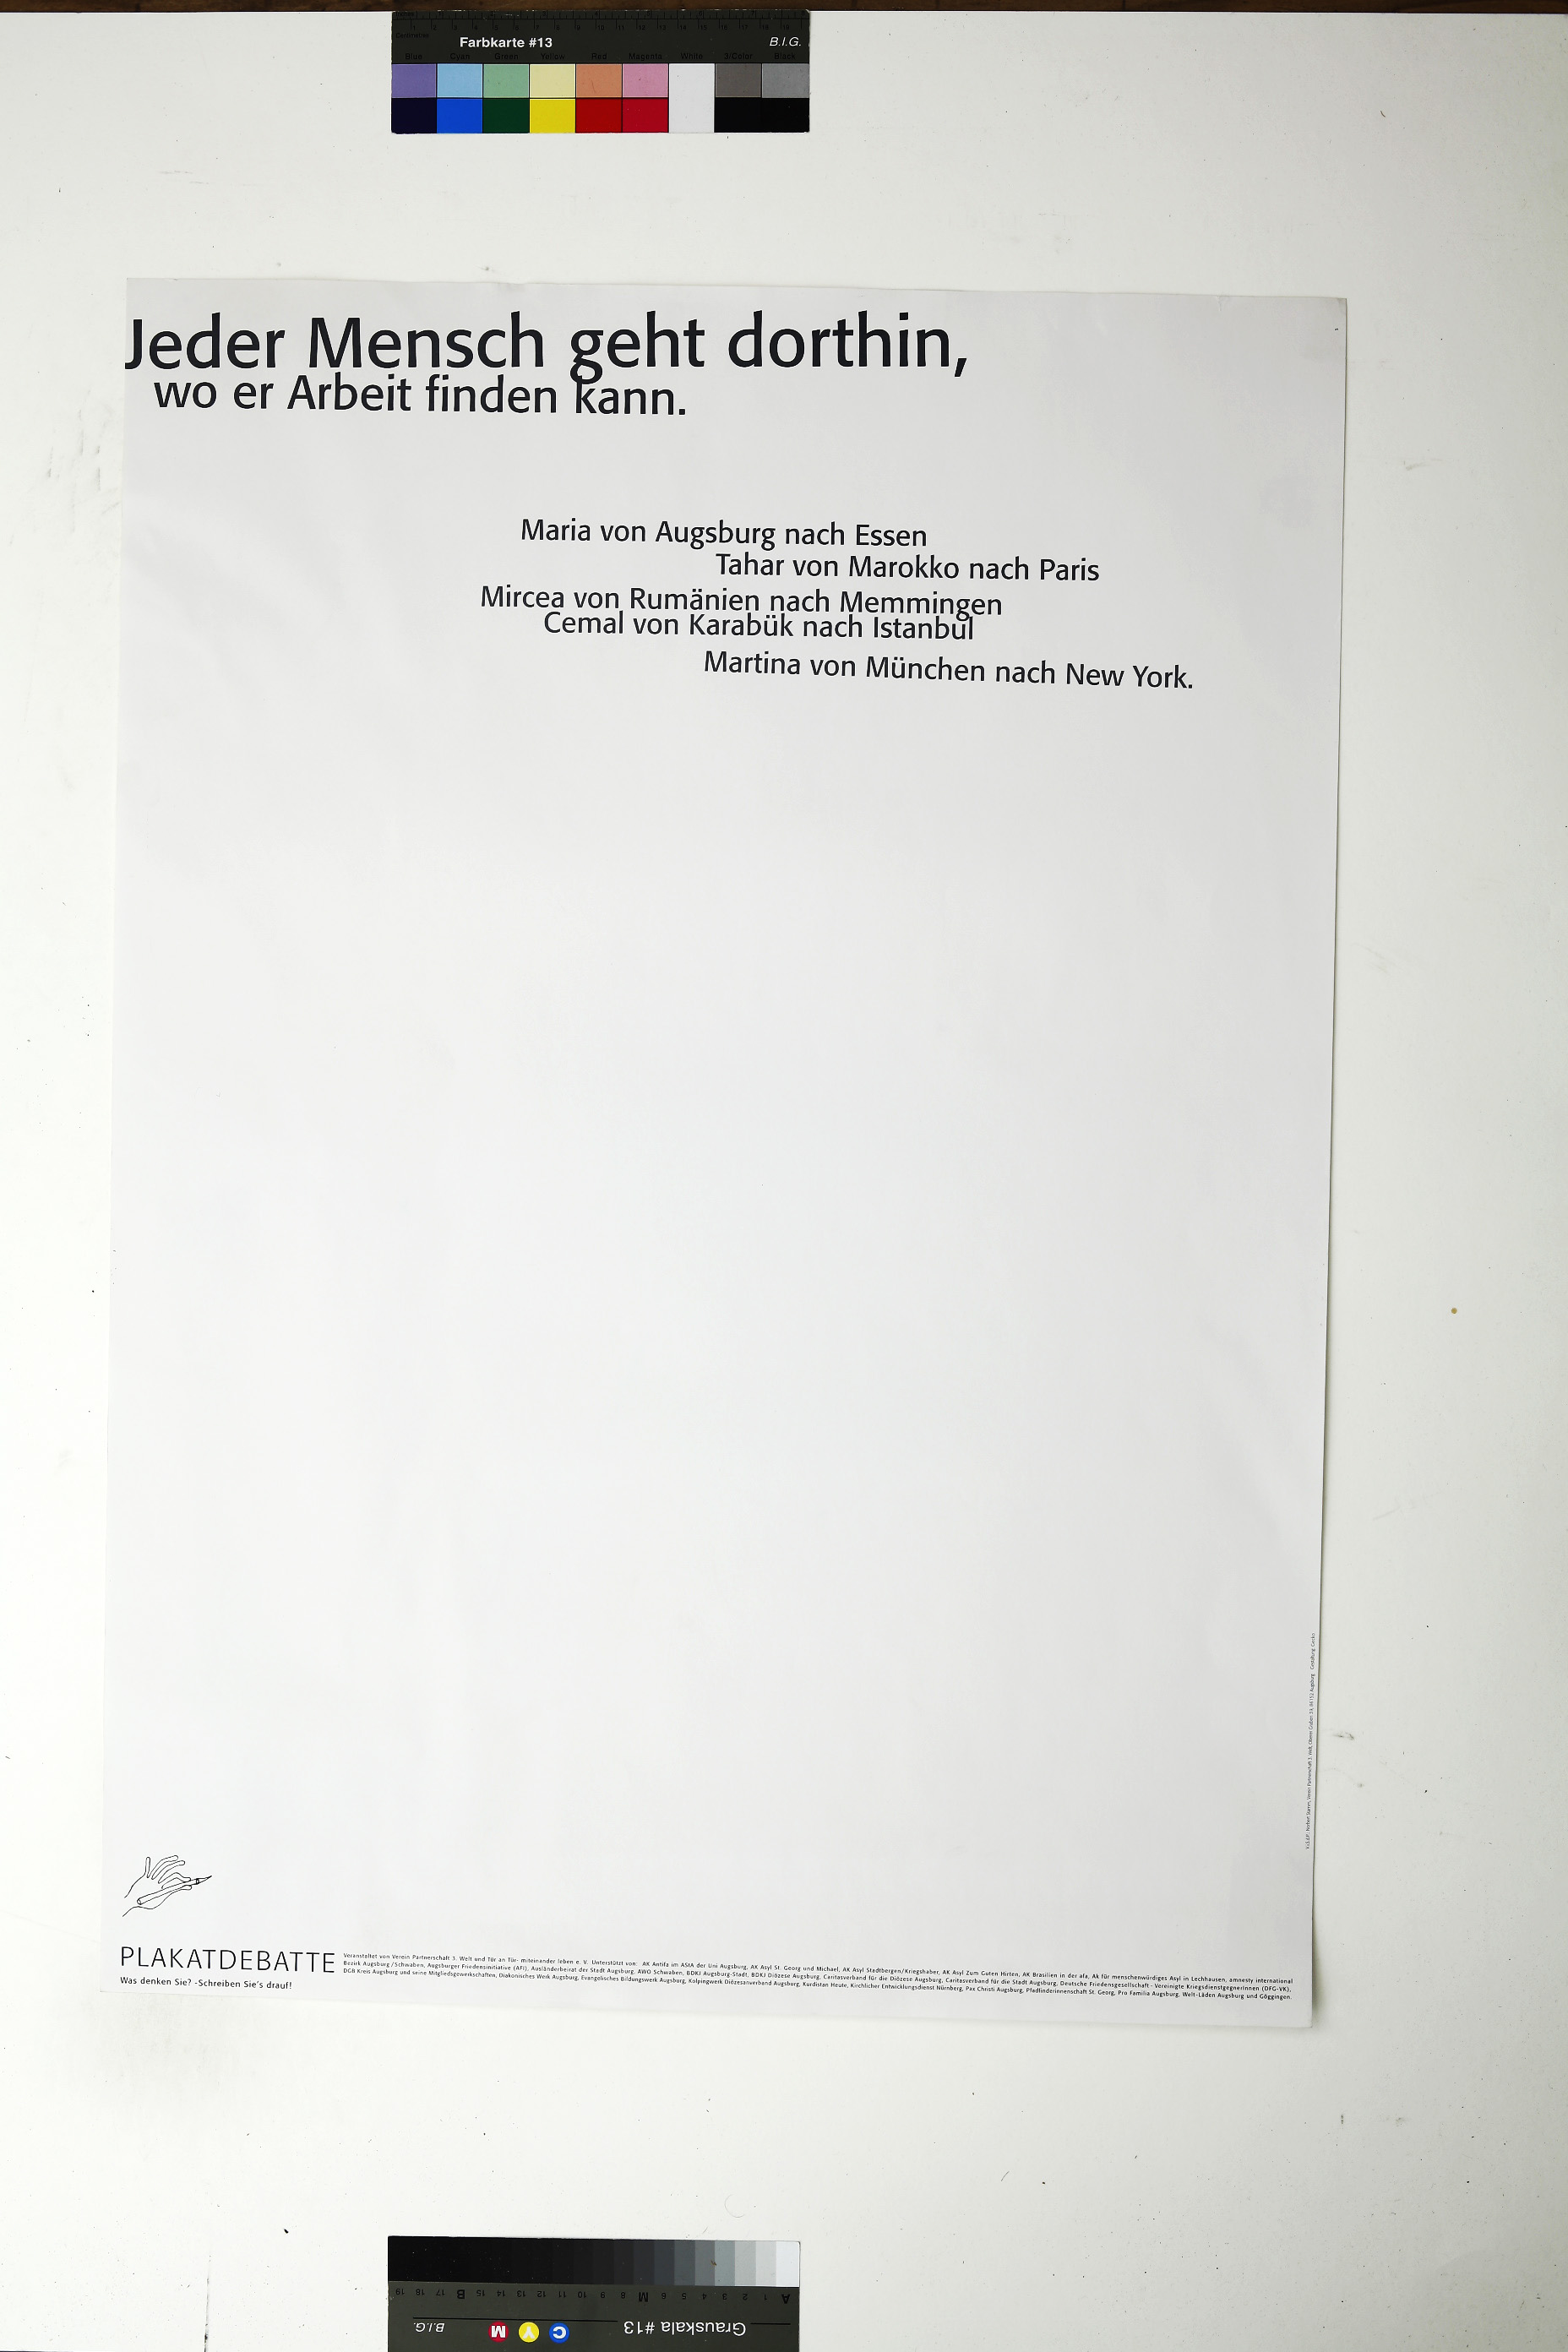
\includegraphics[width=\linewidth]{Abbildung_8b_(acht1_080)}
	\end{subfigure}
	\begin{subfigure}[b]{0.5\linewidth}
	\centering
	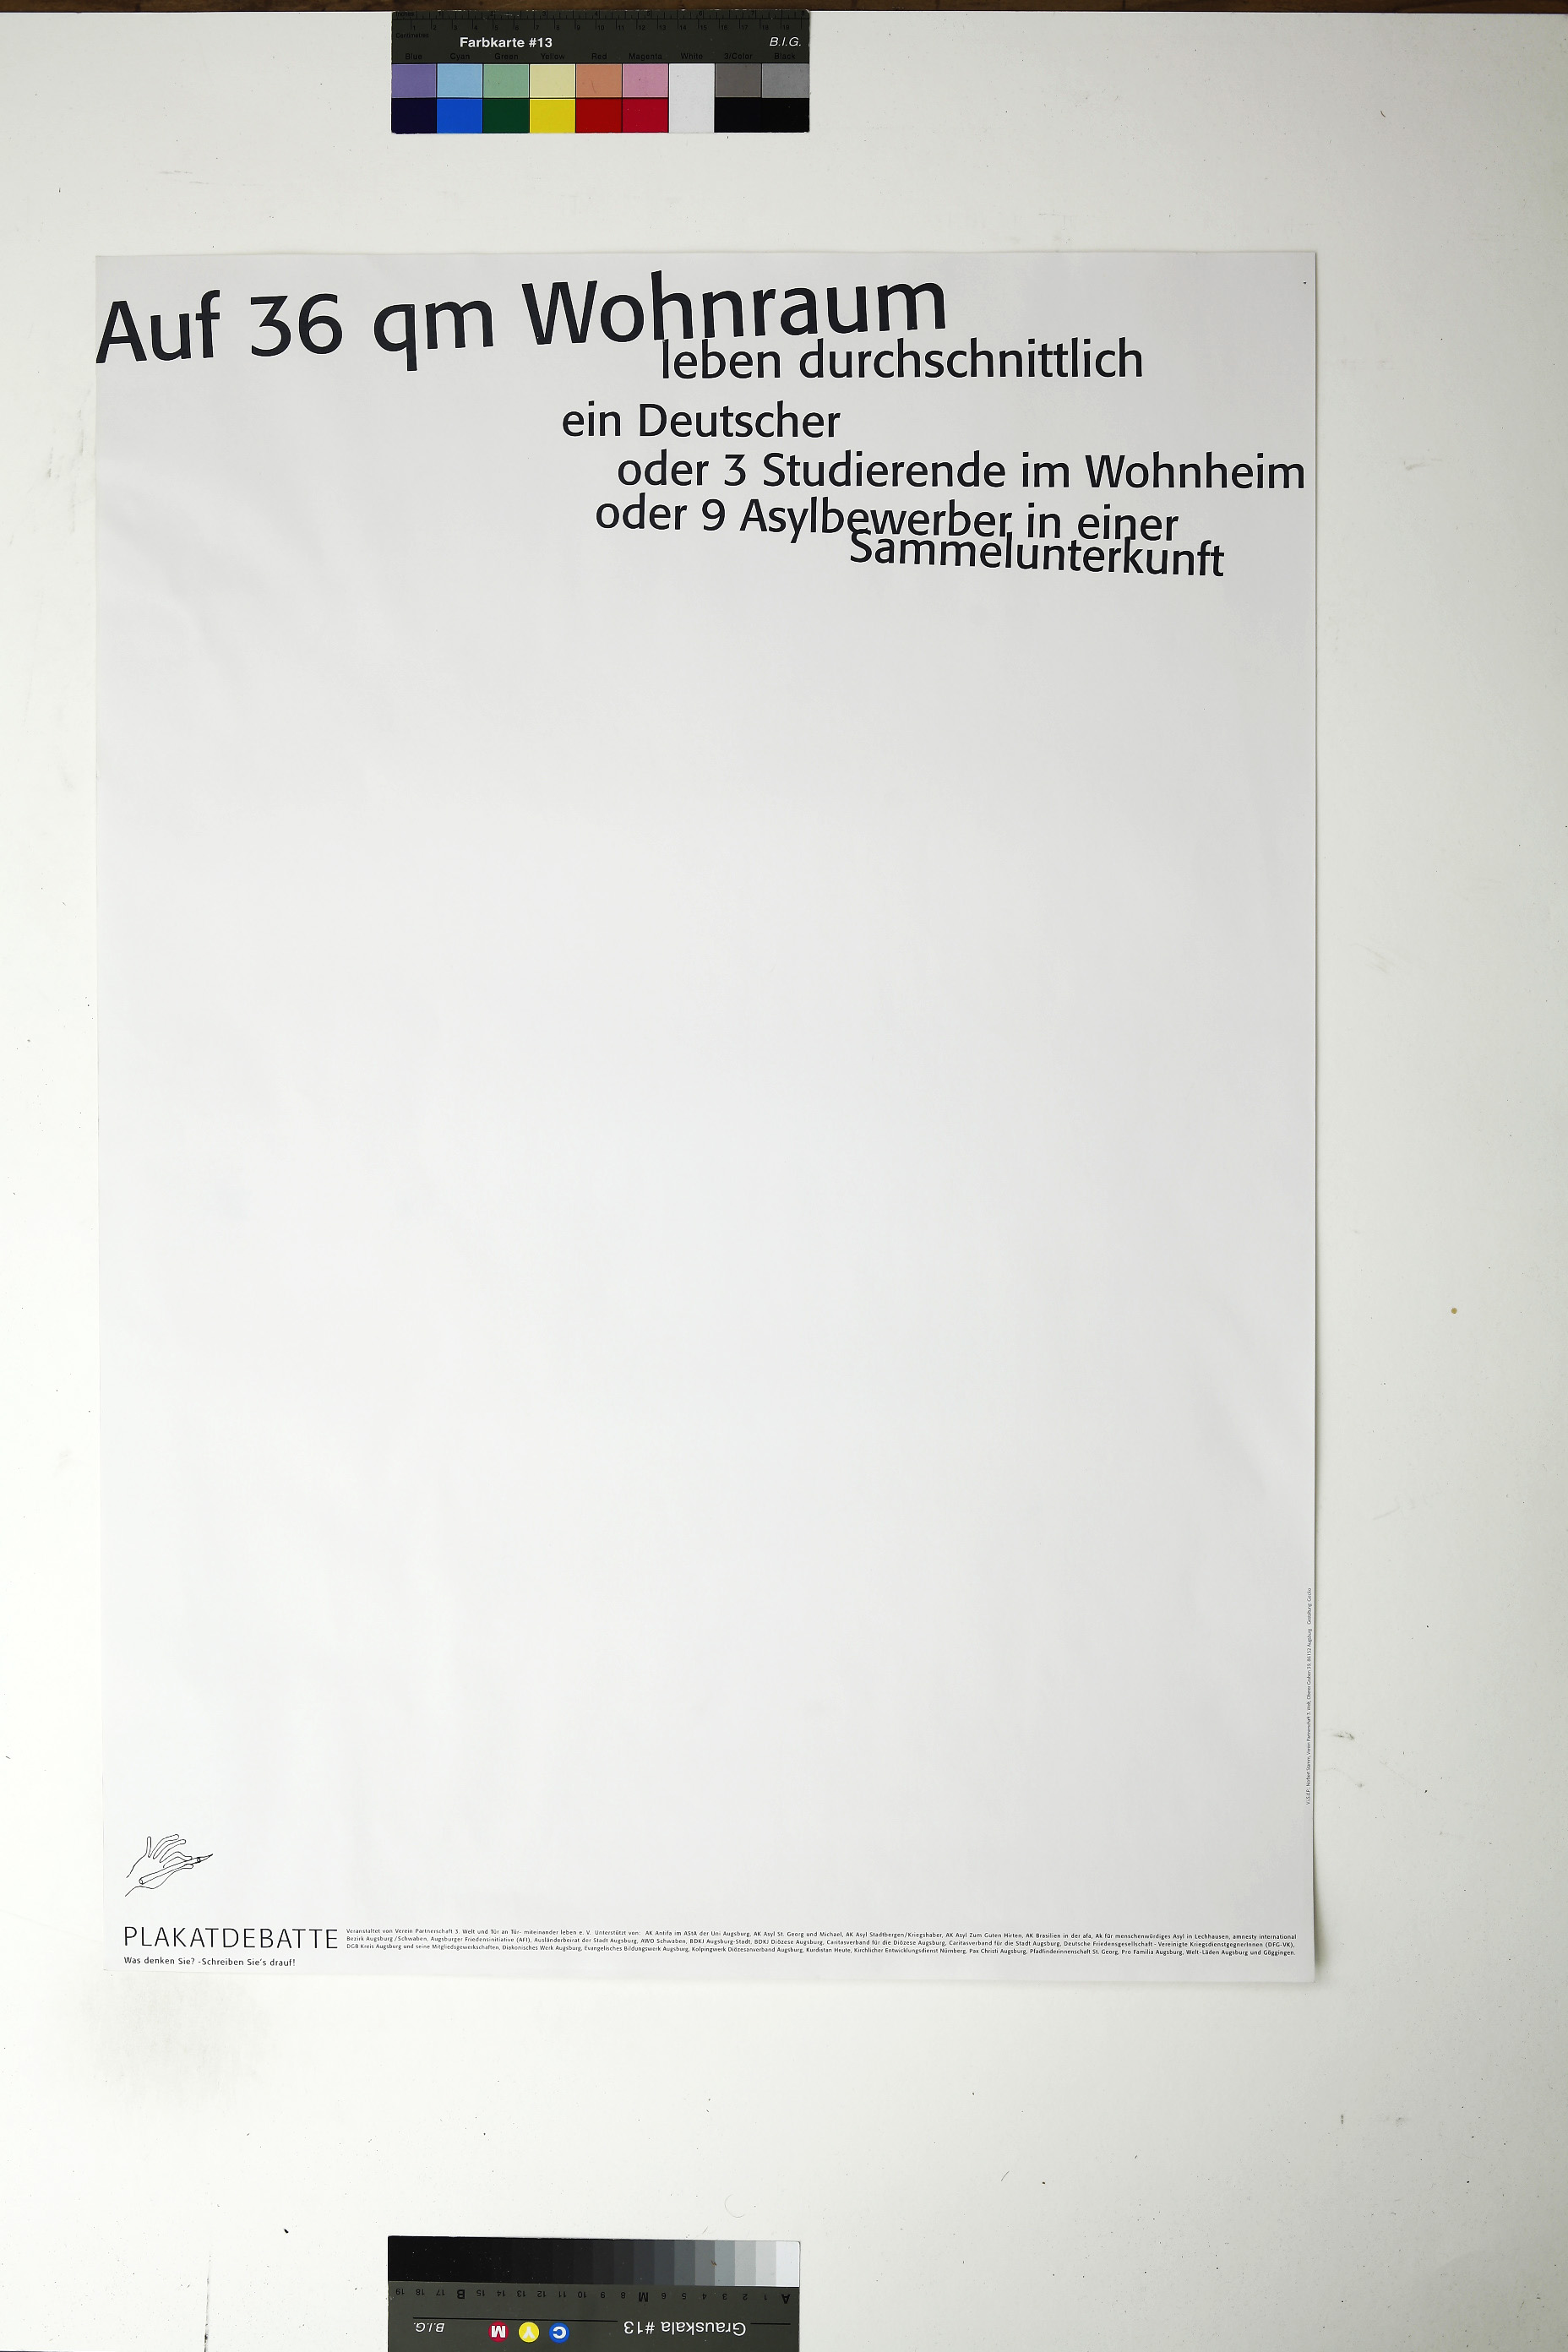
\includegraphics[width=\linewidth]{Abbildung_8c_(acht1_081)}
	\end{subfigure}
	\begin{subfigure}[b]{0.5\linewidth}
	\centering
	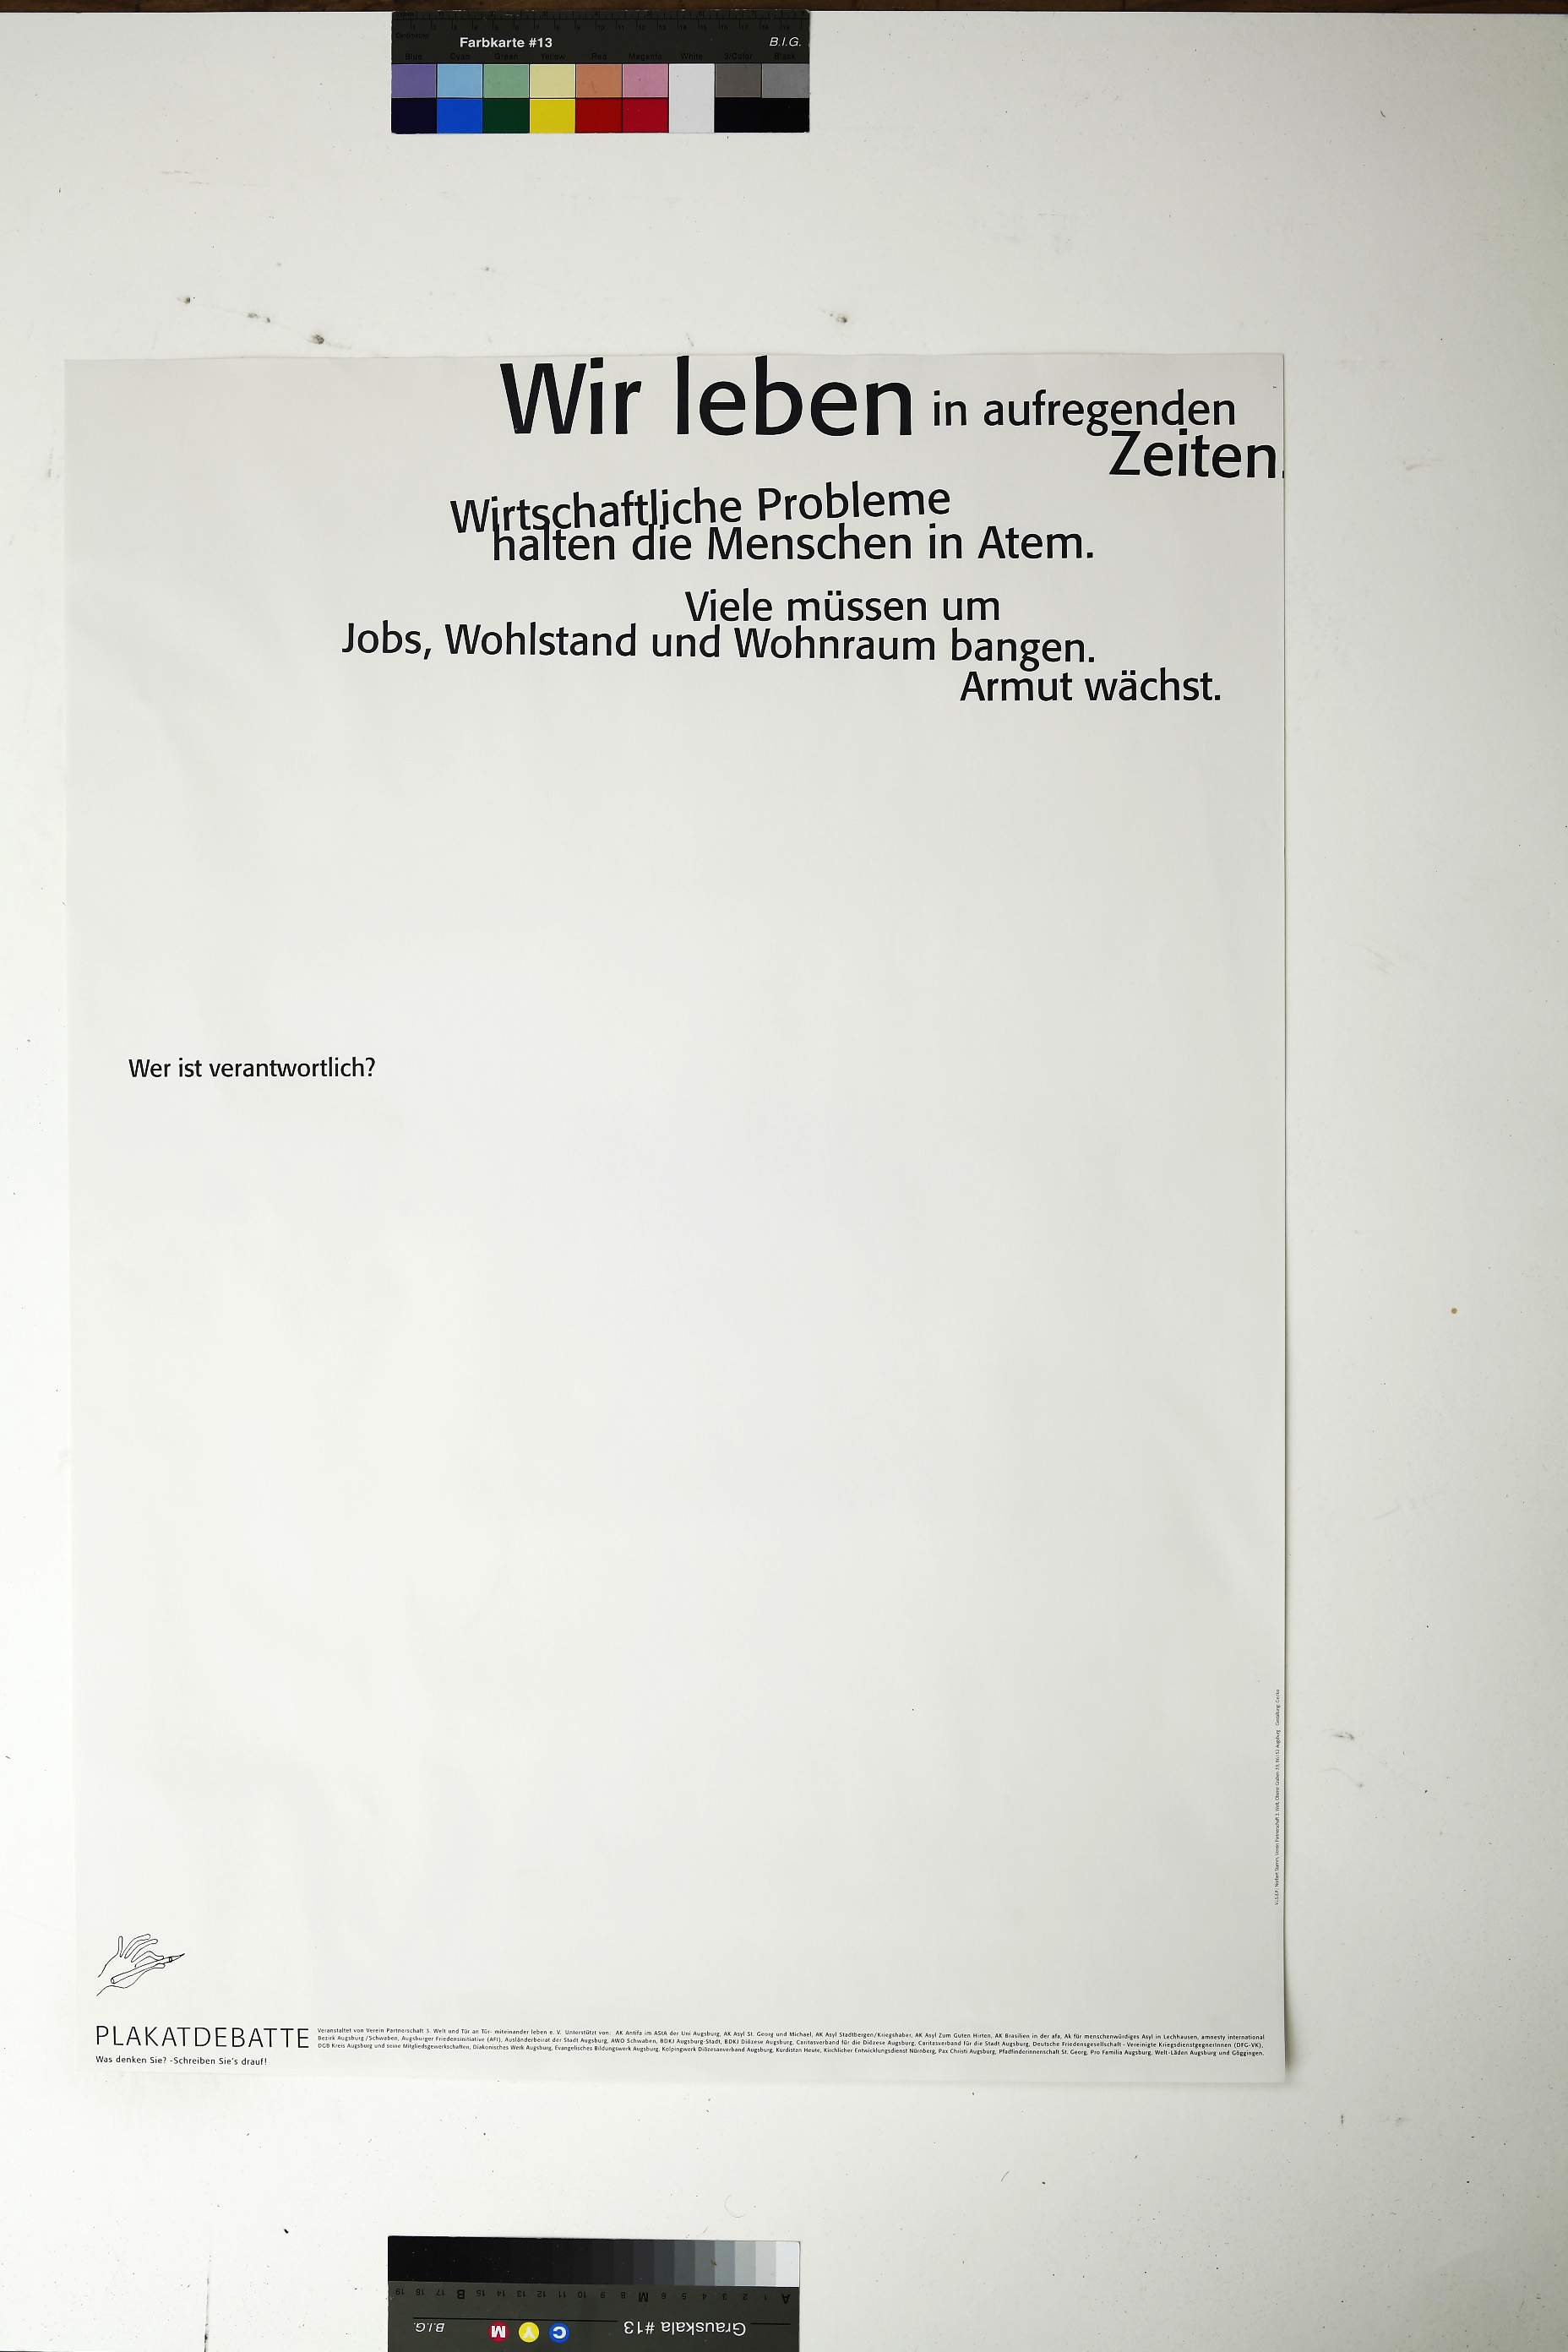
\includegraphics[width=\linewidth]{Abbildung_8d_(acht1_082)}
	\end{subfigure}	
\caption{Vier Beispiele aus der Reihe Plakatdebatte des Vereins „Partnerschaft 3. Welt und Tür an Tür – miteinander leben e. V.“, ohne Datum (acht1\_079, acht1\_080, acht1\_081, acht1\_082).}
\end{figure}

\newpage
\begin{figure}[ht]
\includegraphics[width=\linewidth]{Abbildung_9_(zehn4_209)}
\centering
\caption{Filmplakat – Gran Torino, 2008 (zehn4\_209).}
\end{figure}

\newpage
\begin{figure}[ht]
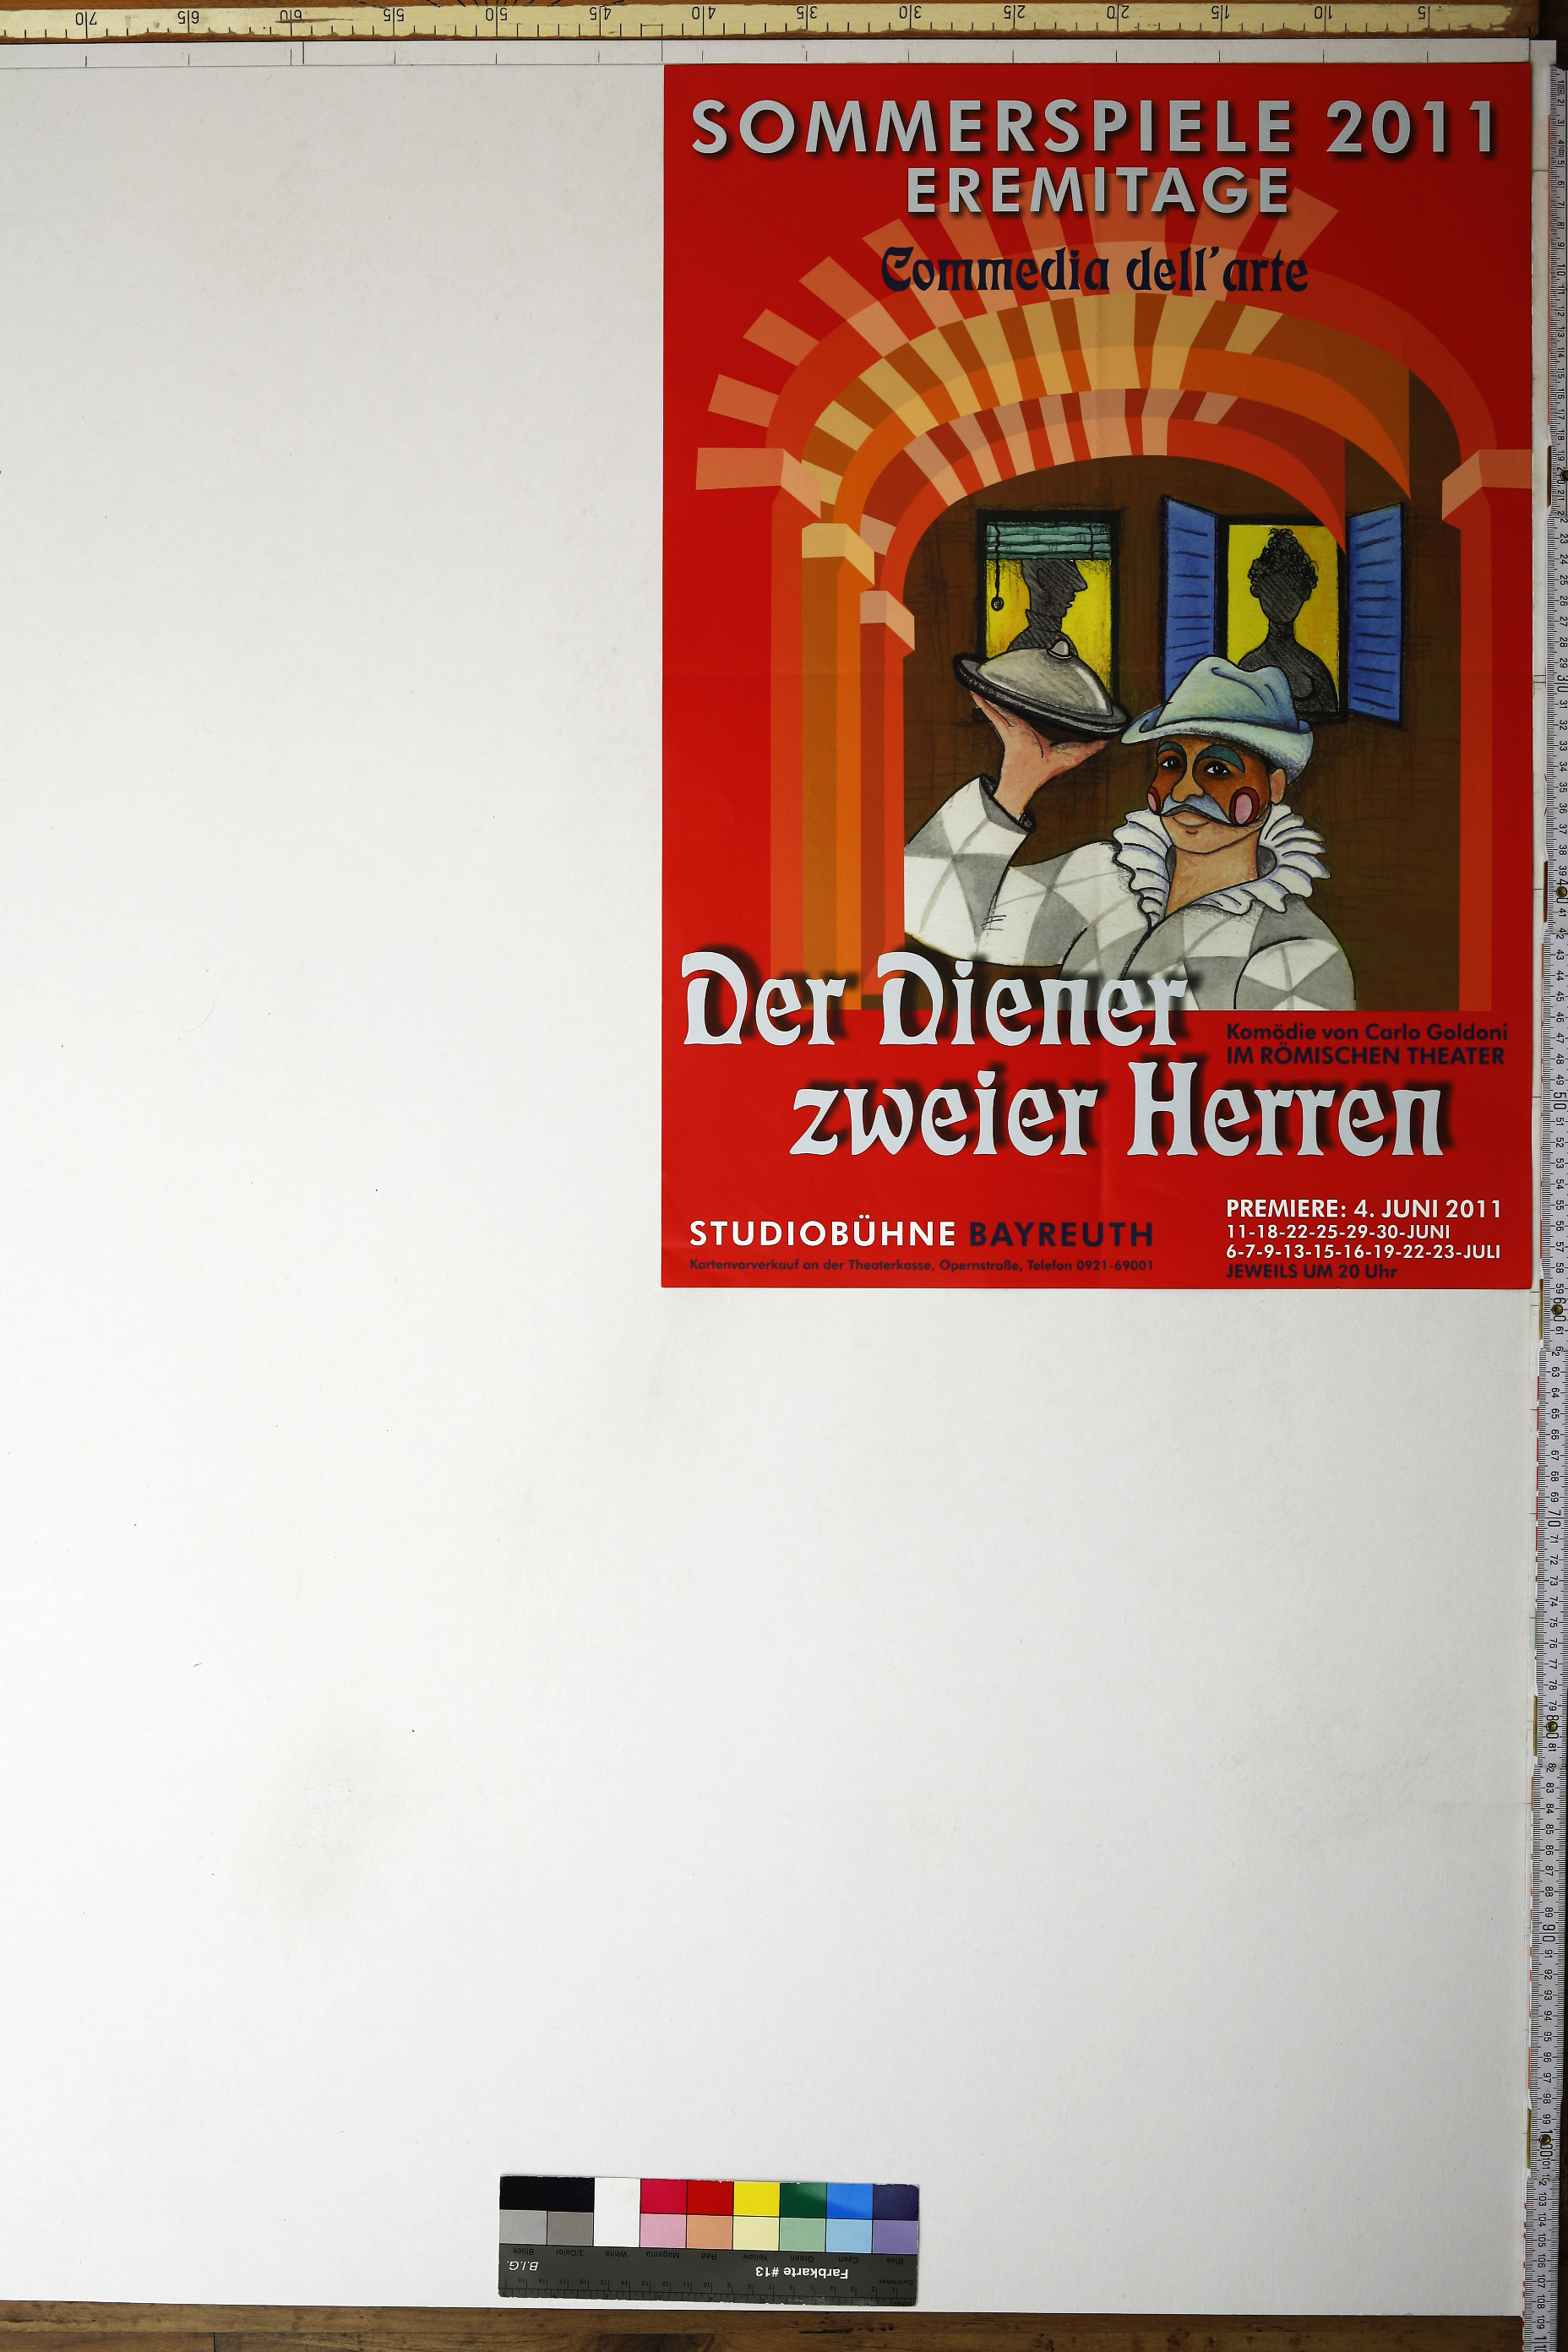
\includegraphics[width=\linewidth]{Abbildung_10_(acht3_299)}
\centering
\caption{Theaterplakat – Der Diener Zweier Herren, Studiobühne Bayreuth, 04.06.2011 (acht3\_299).}
\end{figure}

\newpage
\begin{figure}[ht]
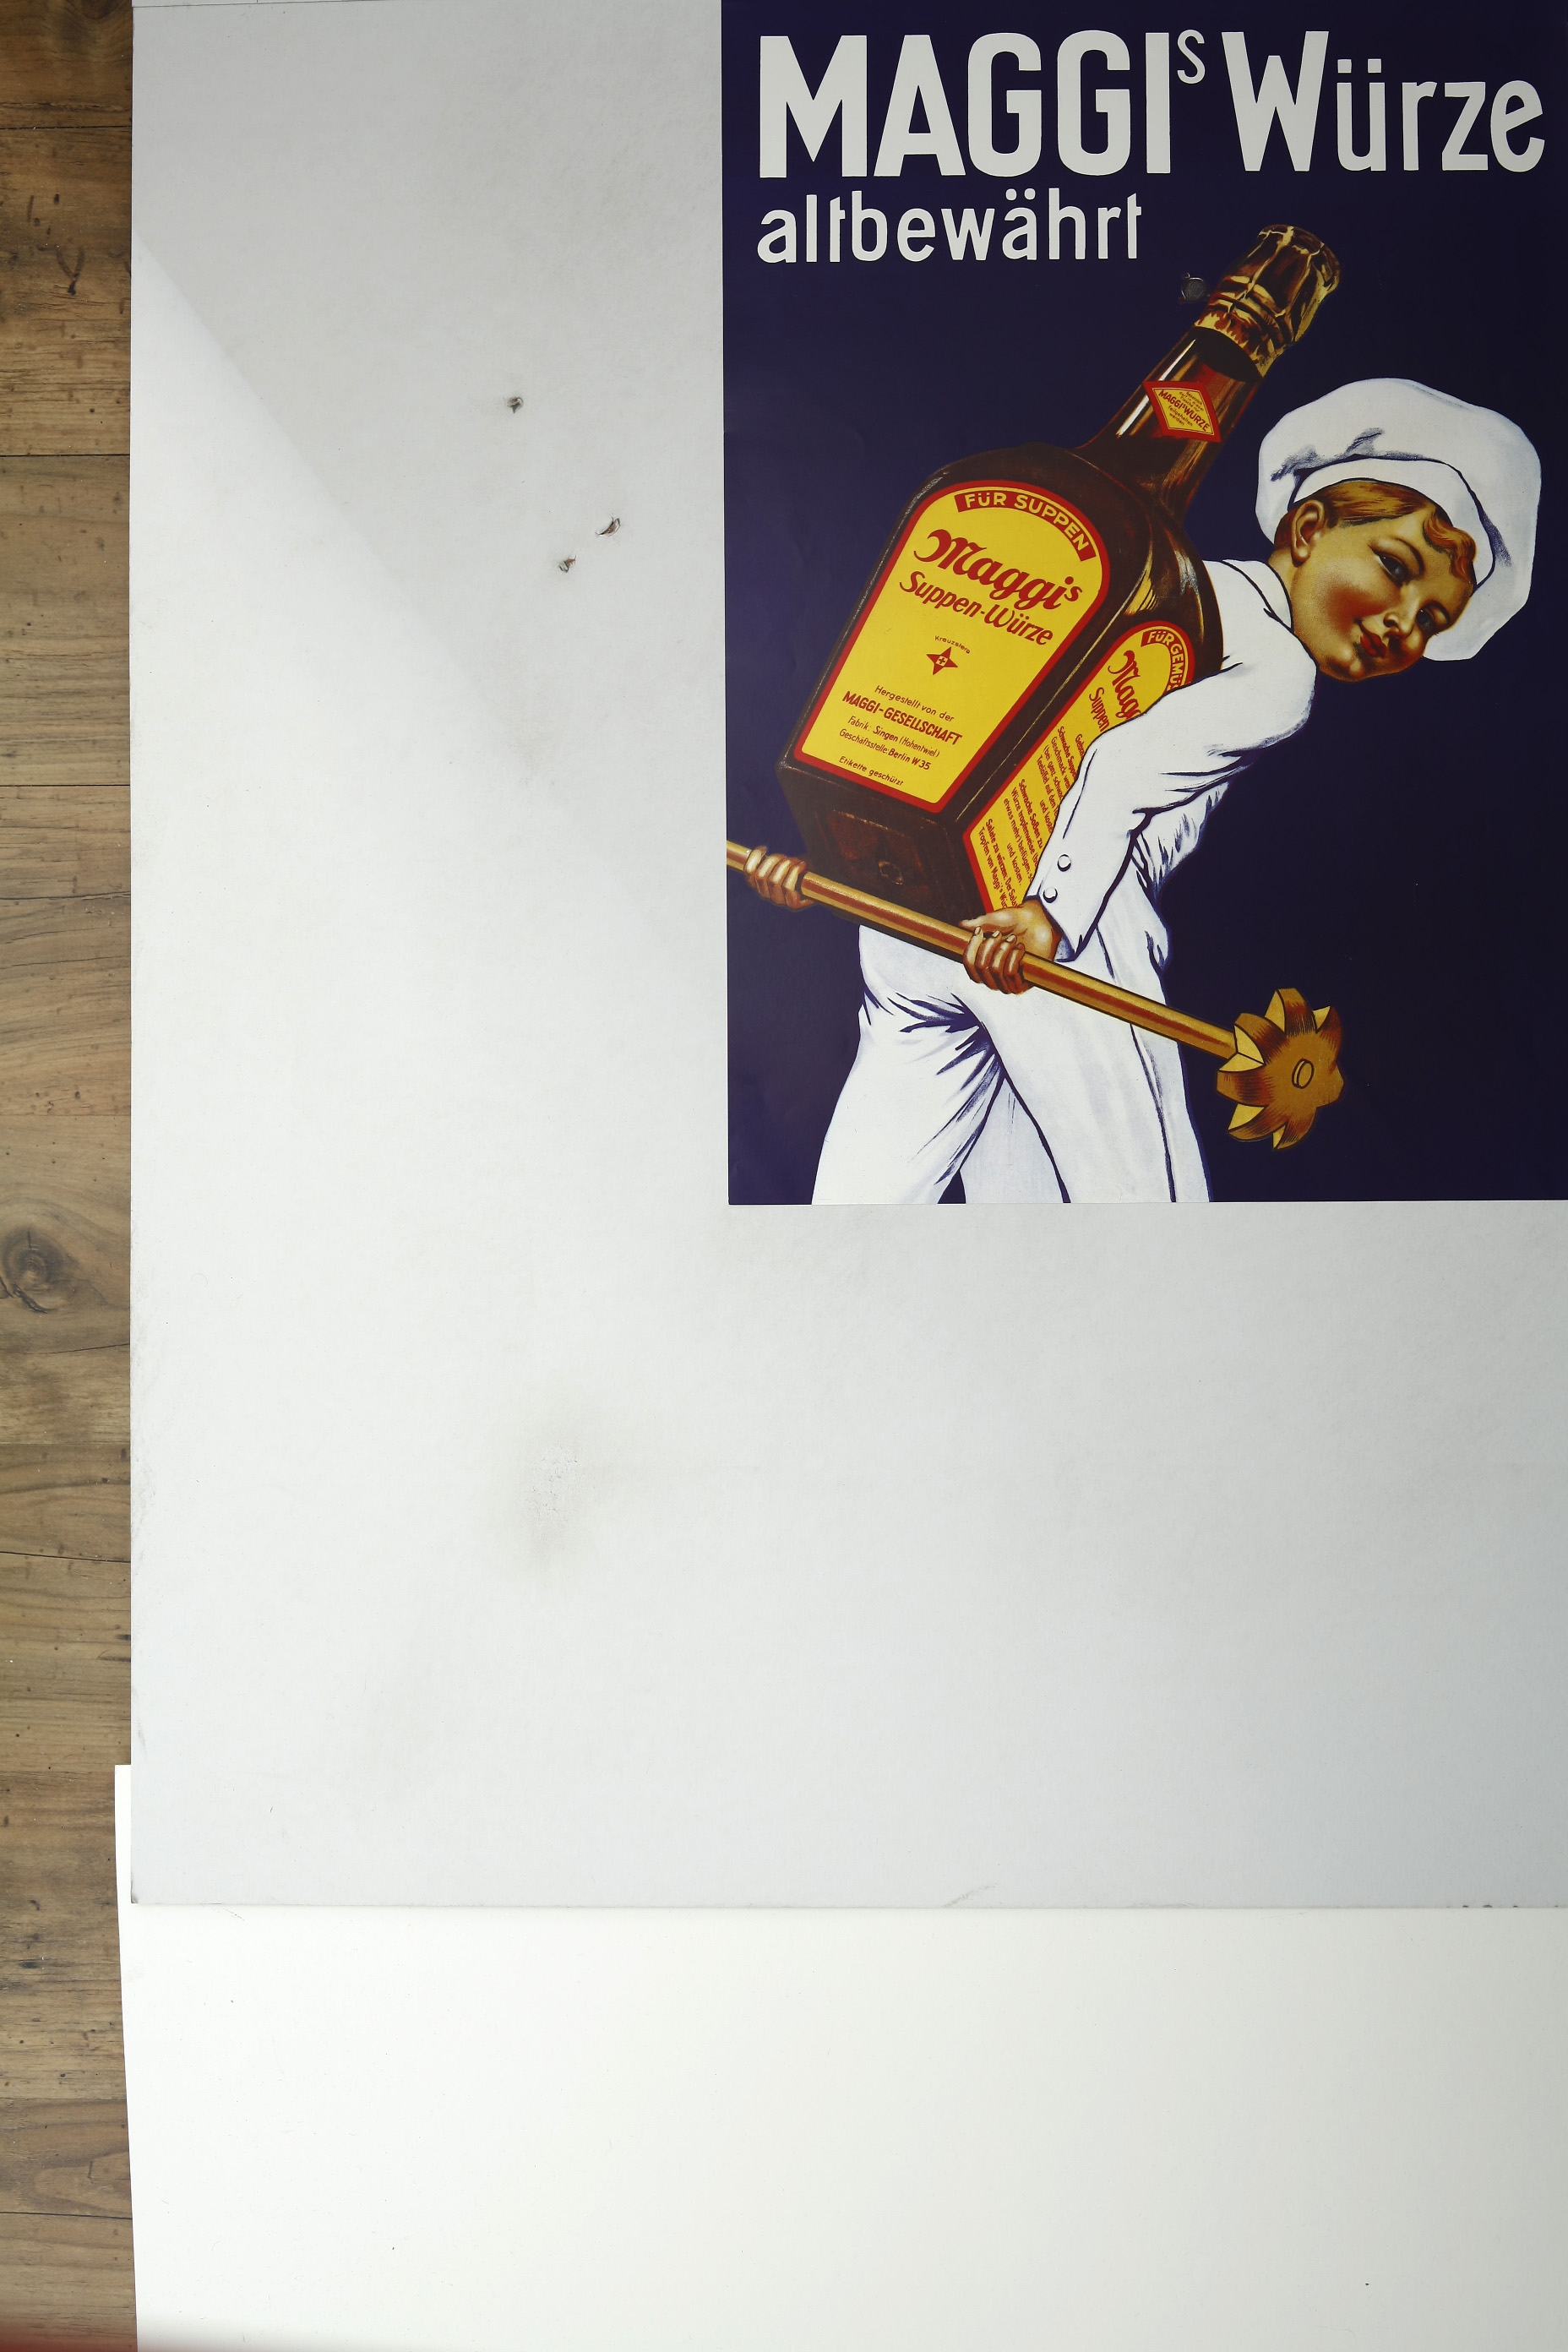
\includegraphics[width=\linewidth]{Abbildung_11_(sechzehn7_002)}
\centering
\caption{Werbeplakat – Maggis Würze altbewährt, Maggi, ohne Datum (sechzehn7\_002).}
\end{figure}

\newpage
\begin{figure}[ht]
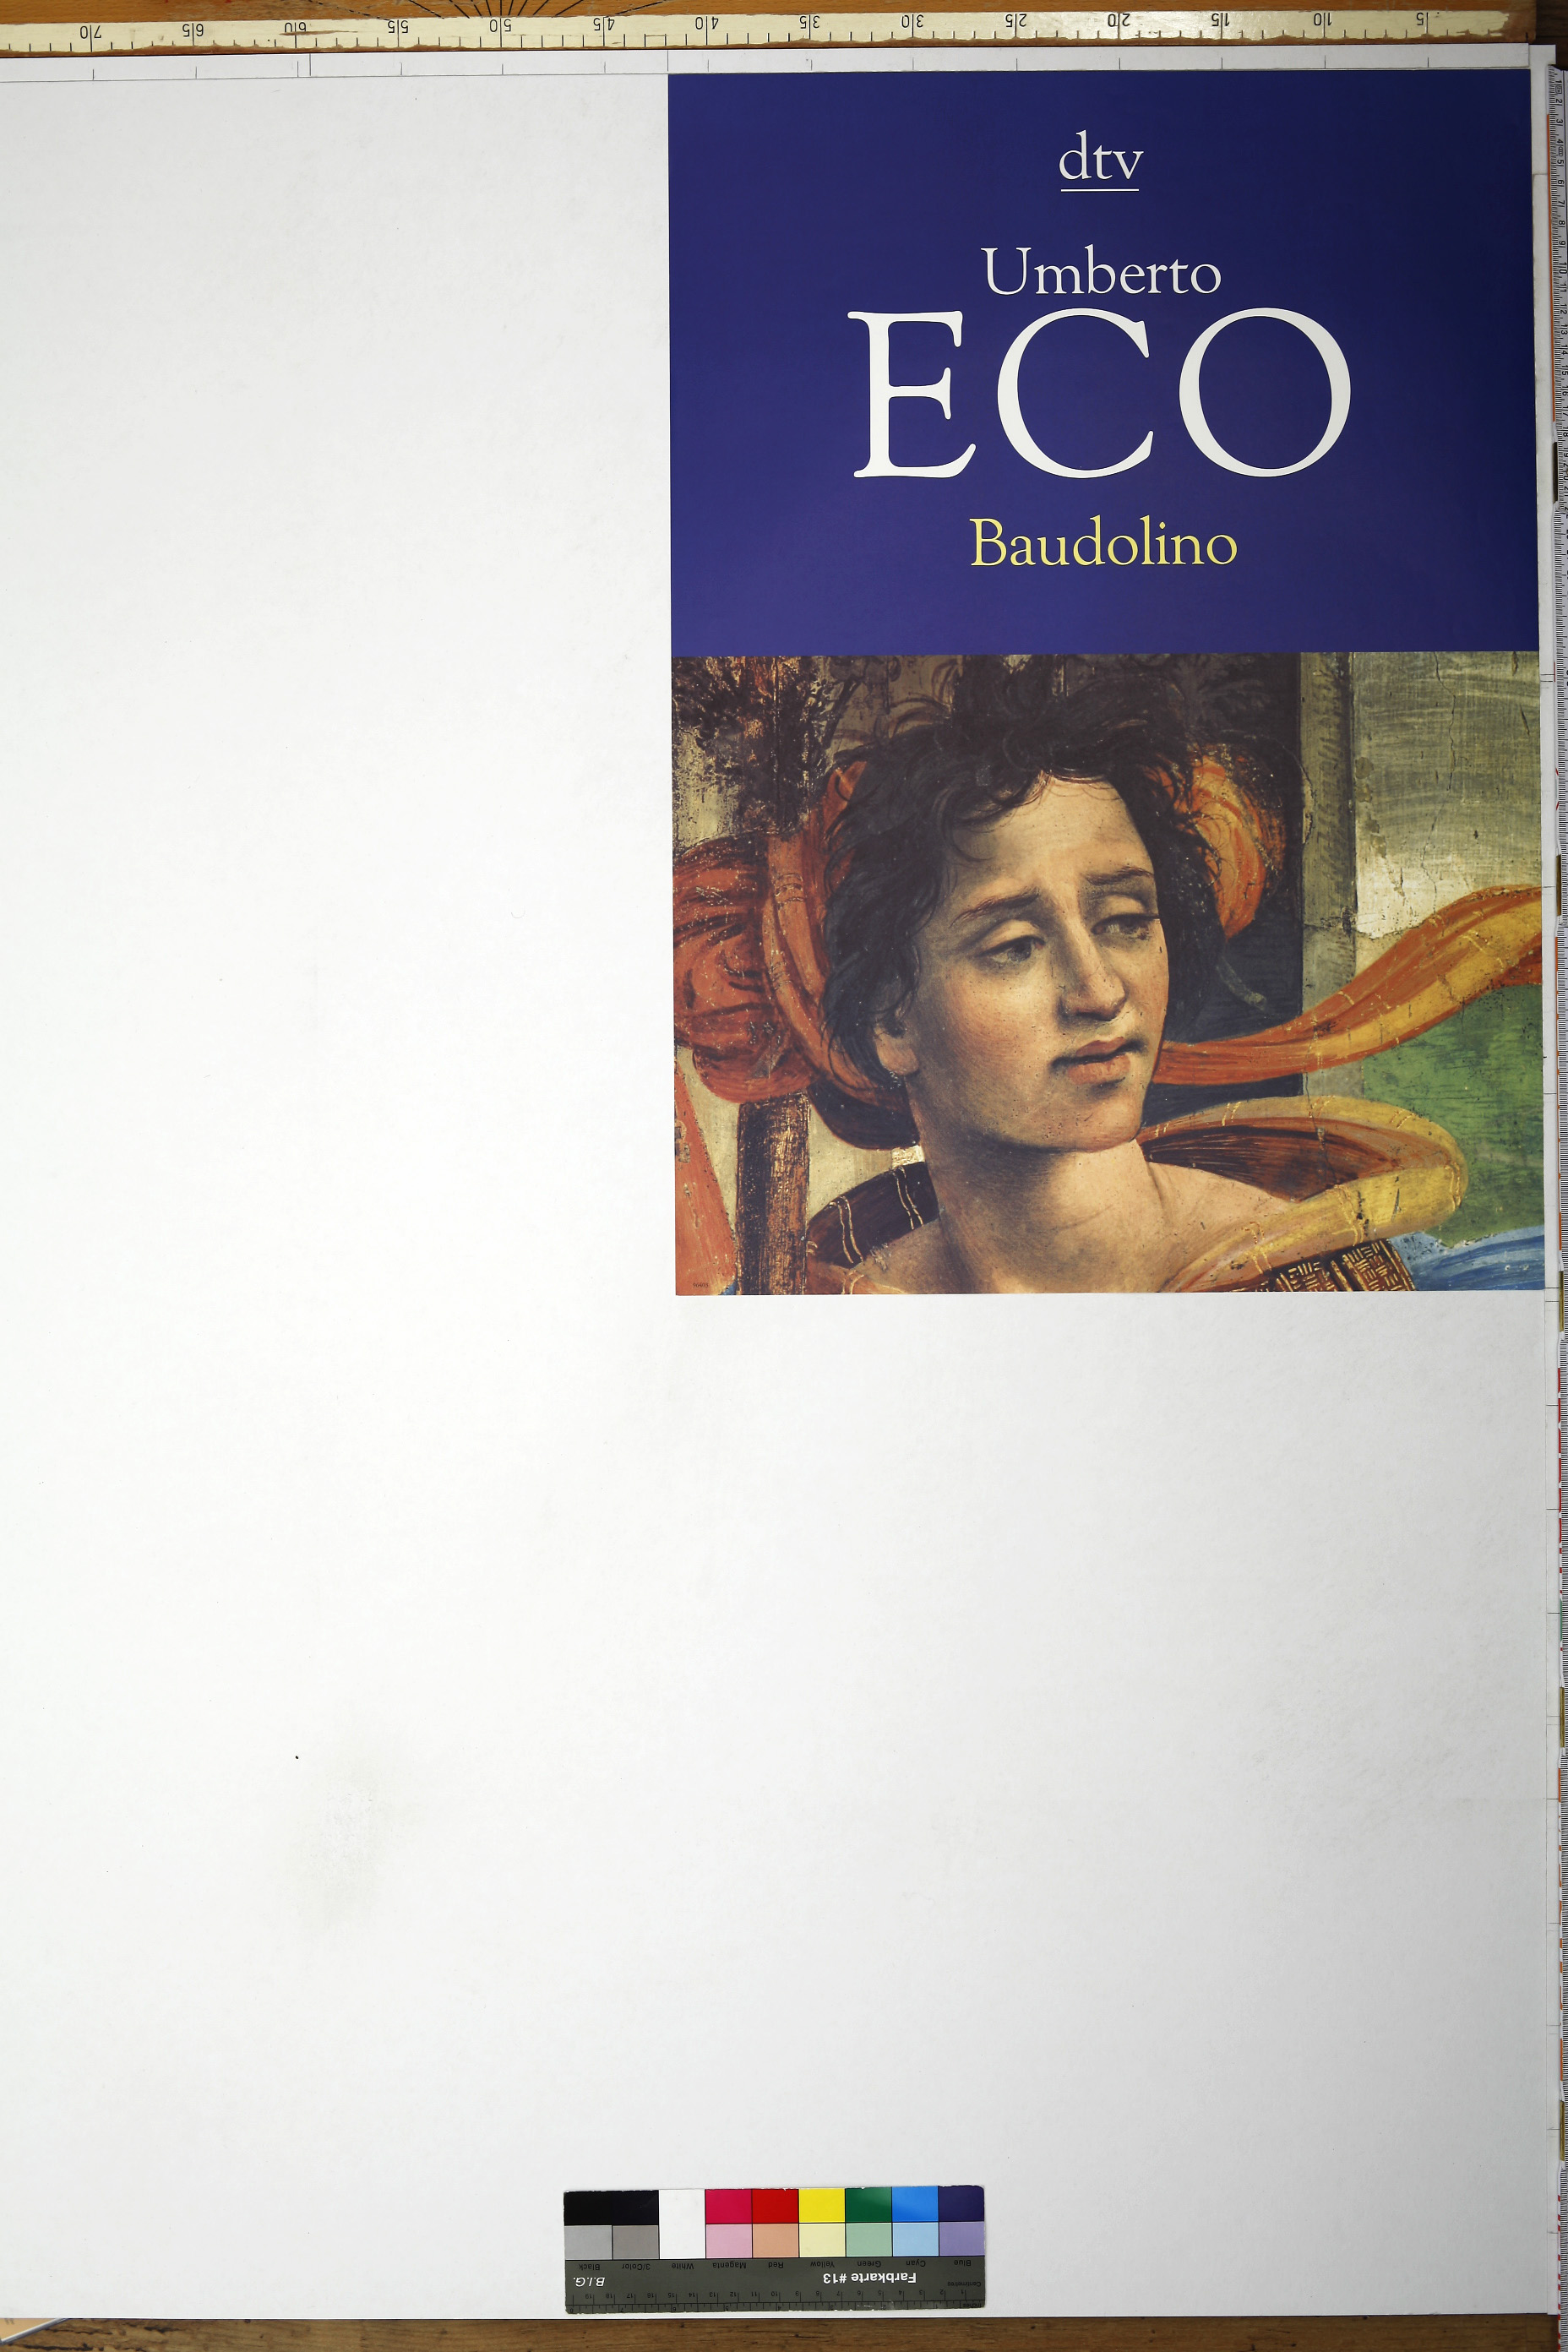
\includegraphics[width=\linewidth]{Abbildung_12_(acht3_020)}
\centering
\caption{Buchplakat – Umberto Eco: Baudolino, dtv, ohne Datum (acht3\_020).}
\end{figure}

\newpage
\begin{figure}[ht]
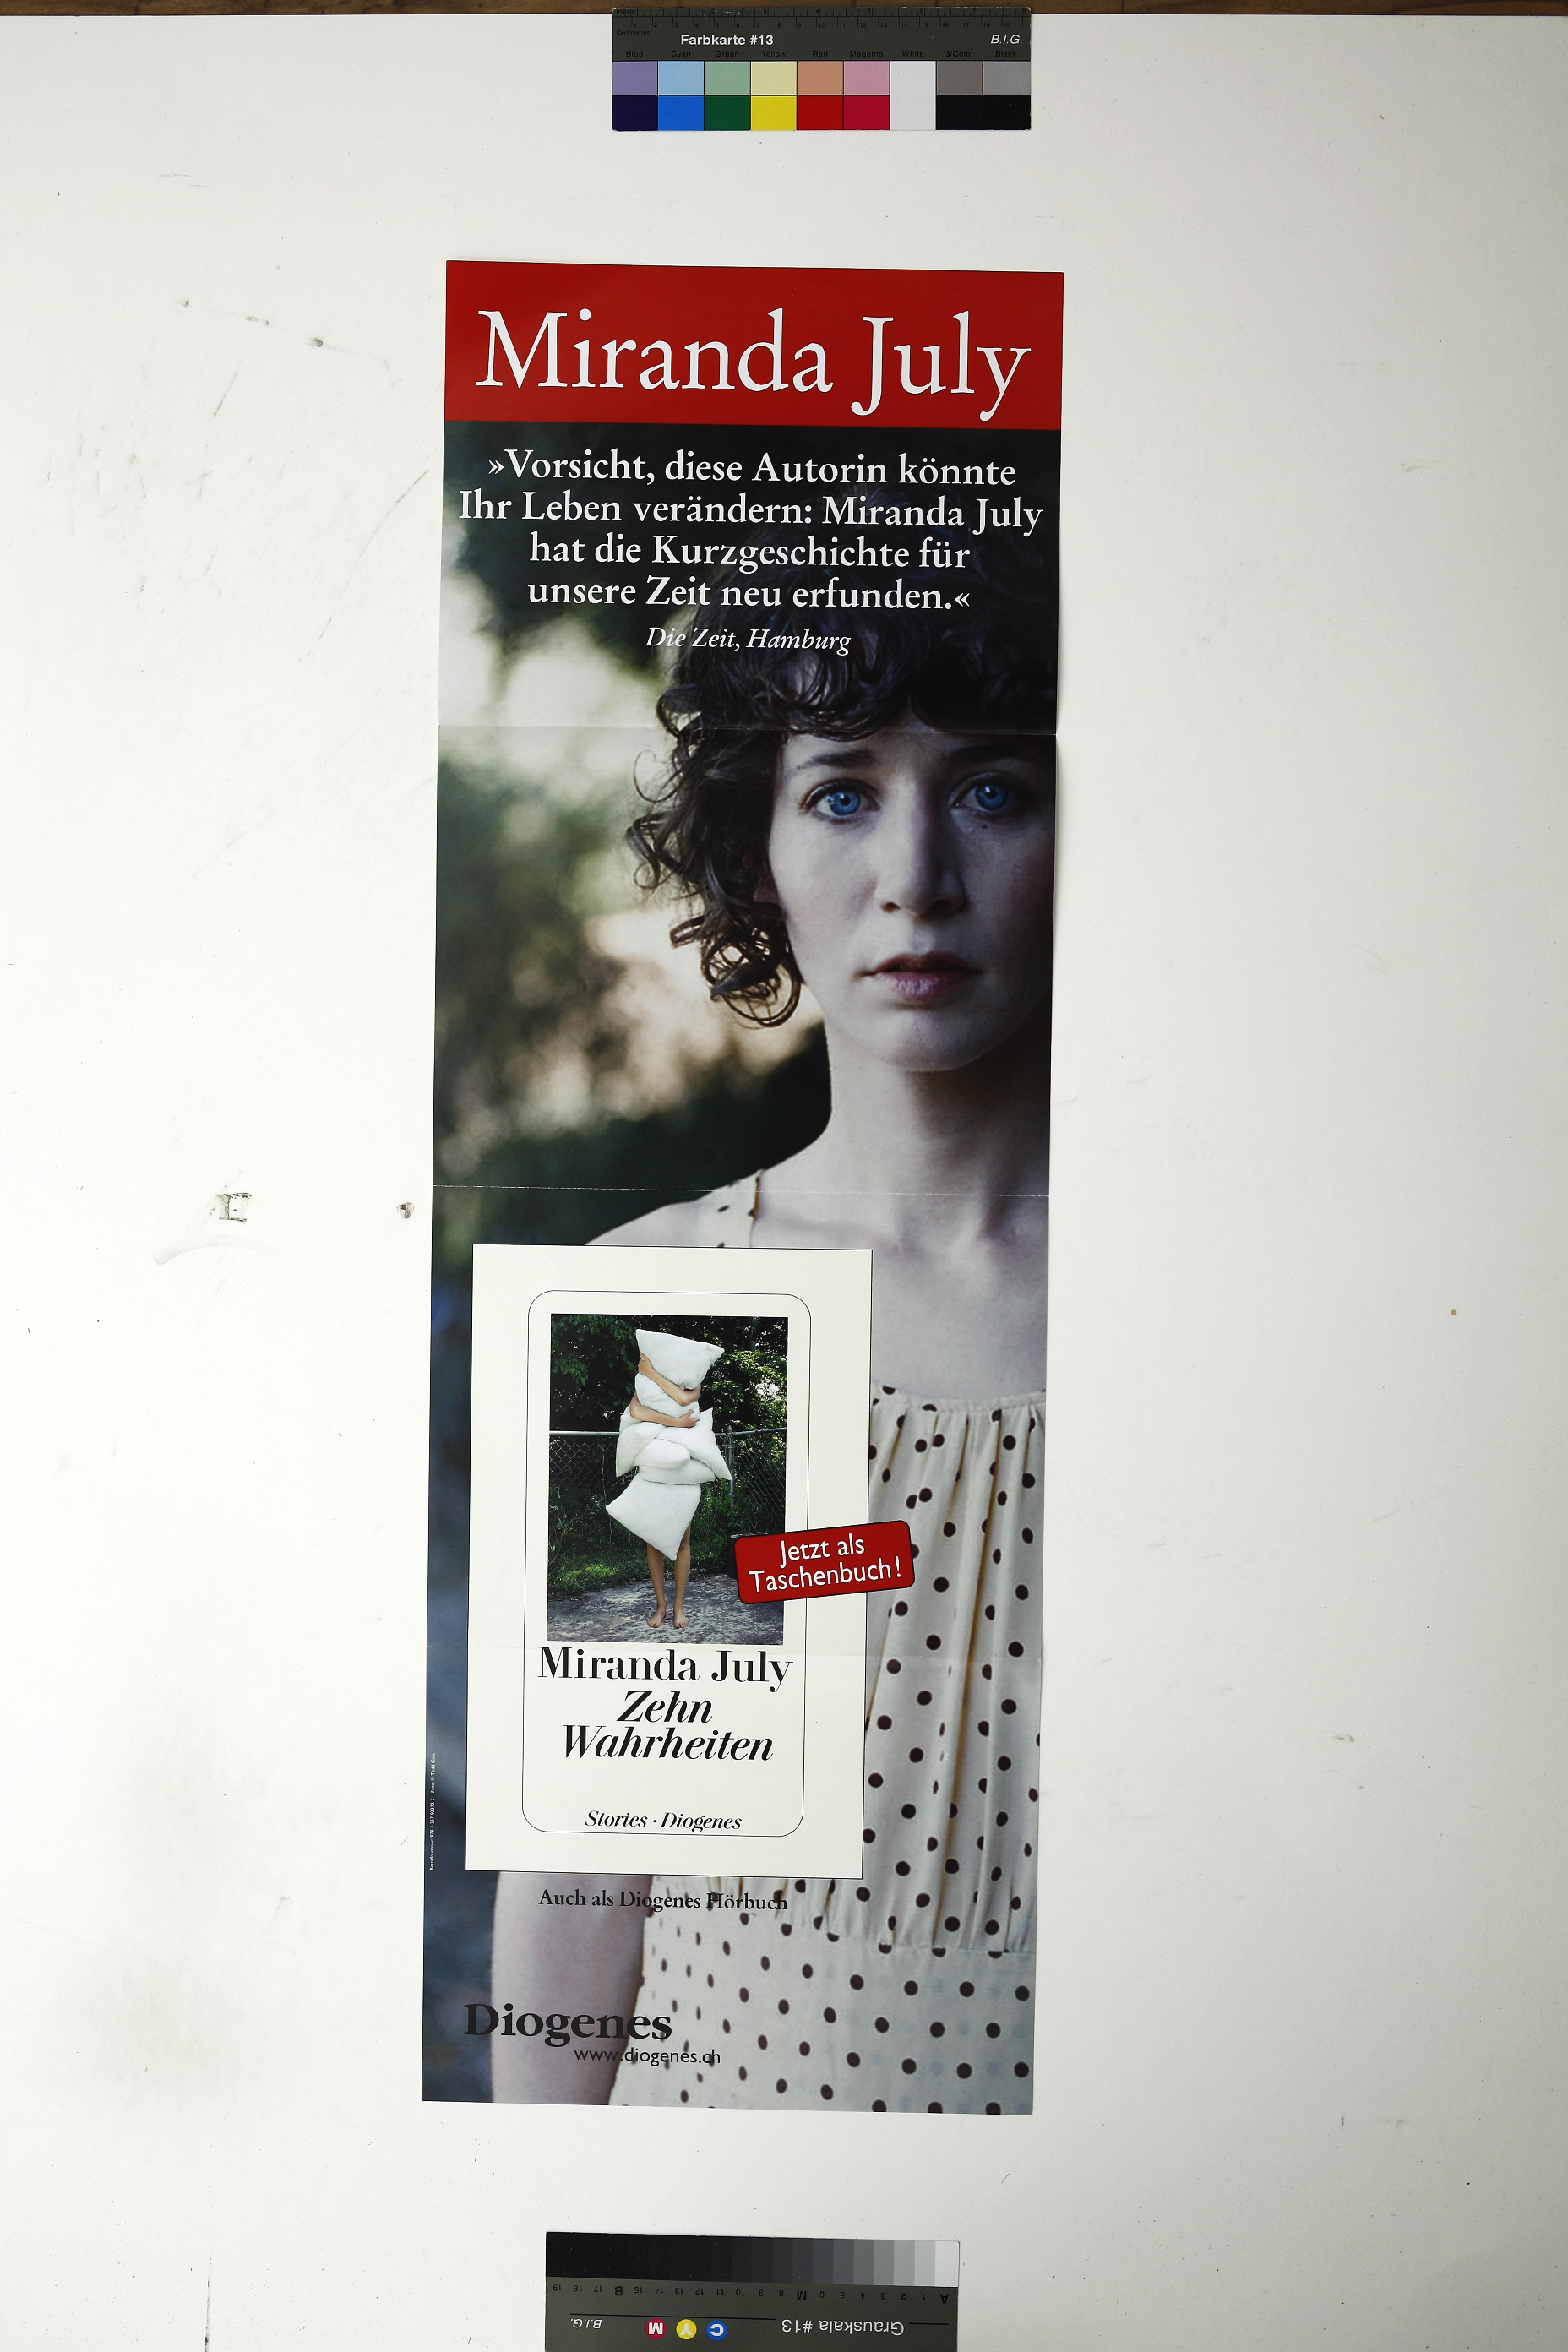
\includegraphics[width=\linewidth]{Abbildung_13_(acht2_172)}
\centering
\caption{Buchplakat – Miranda July: Zehn Wahrheiten, Diogenes, Ohne Datum (acht2\_172).}
\end{figure}

\newpage
\begin{figure}[ht]
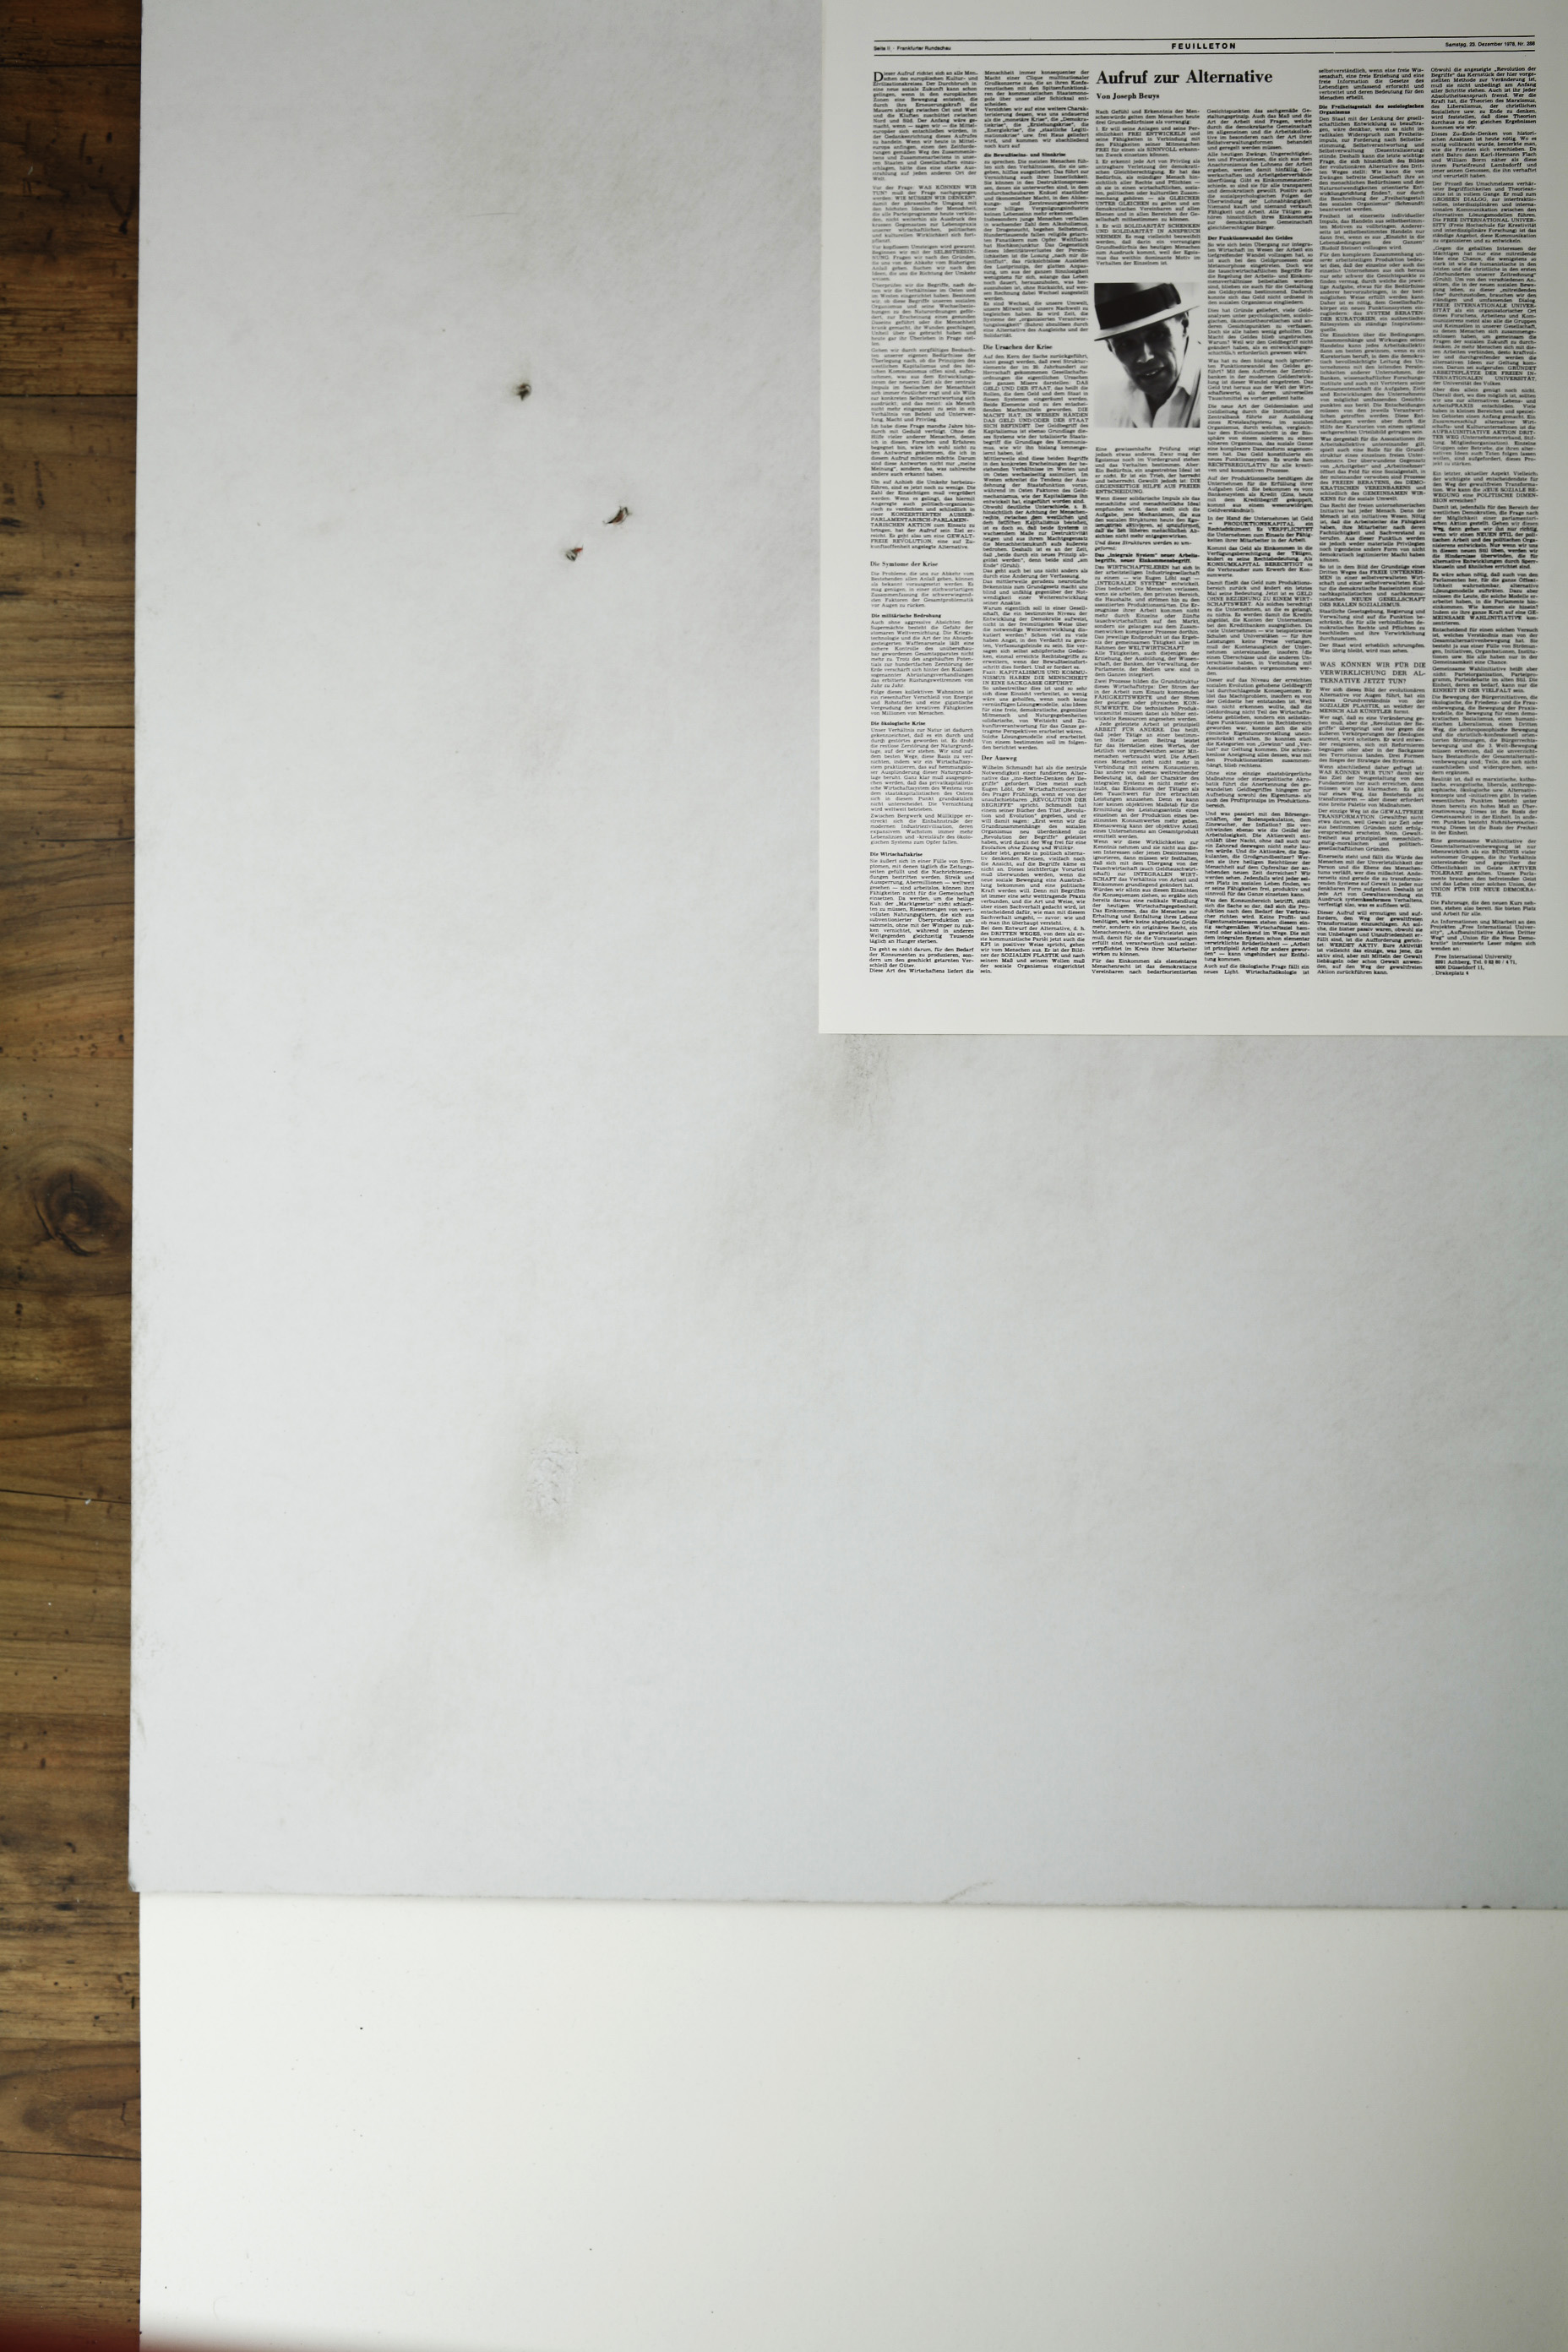
\includegraphics[width=\linewidth]{Abbildung_14_(Sechzehn9_027)}
\centering
\caption{Scan eines Zeitungsausschnitts in der Plakatsammlung (Sechzehn9\_027).}
\end{figure}

\newpage
\begin{figure}[ht]
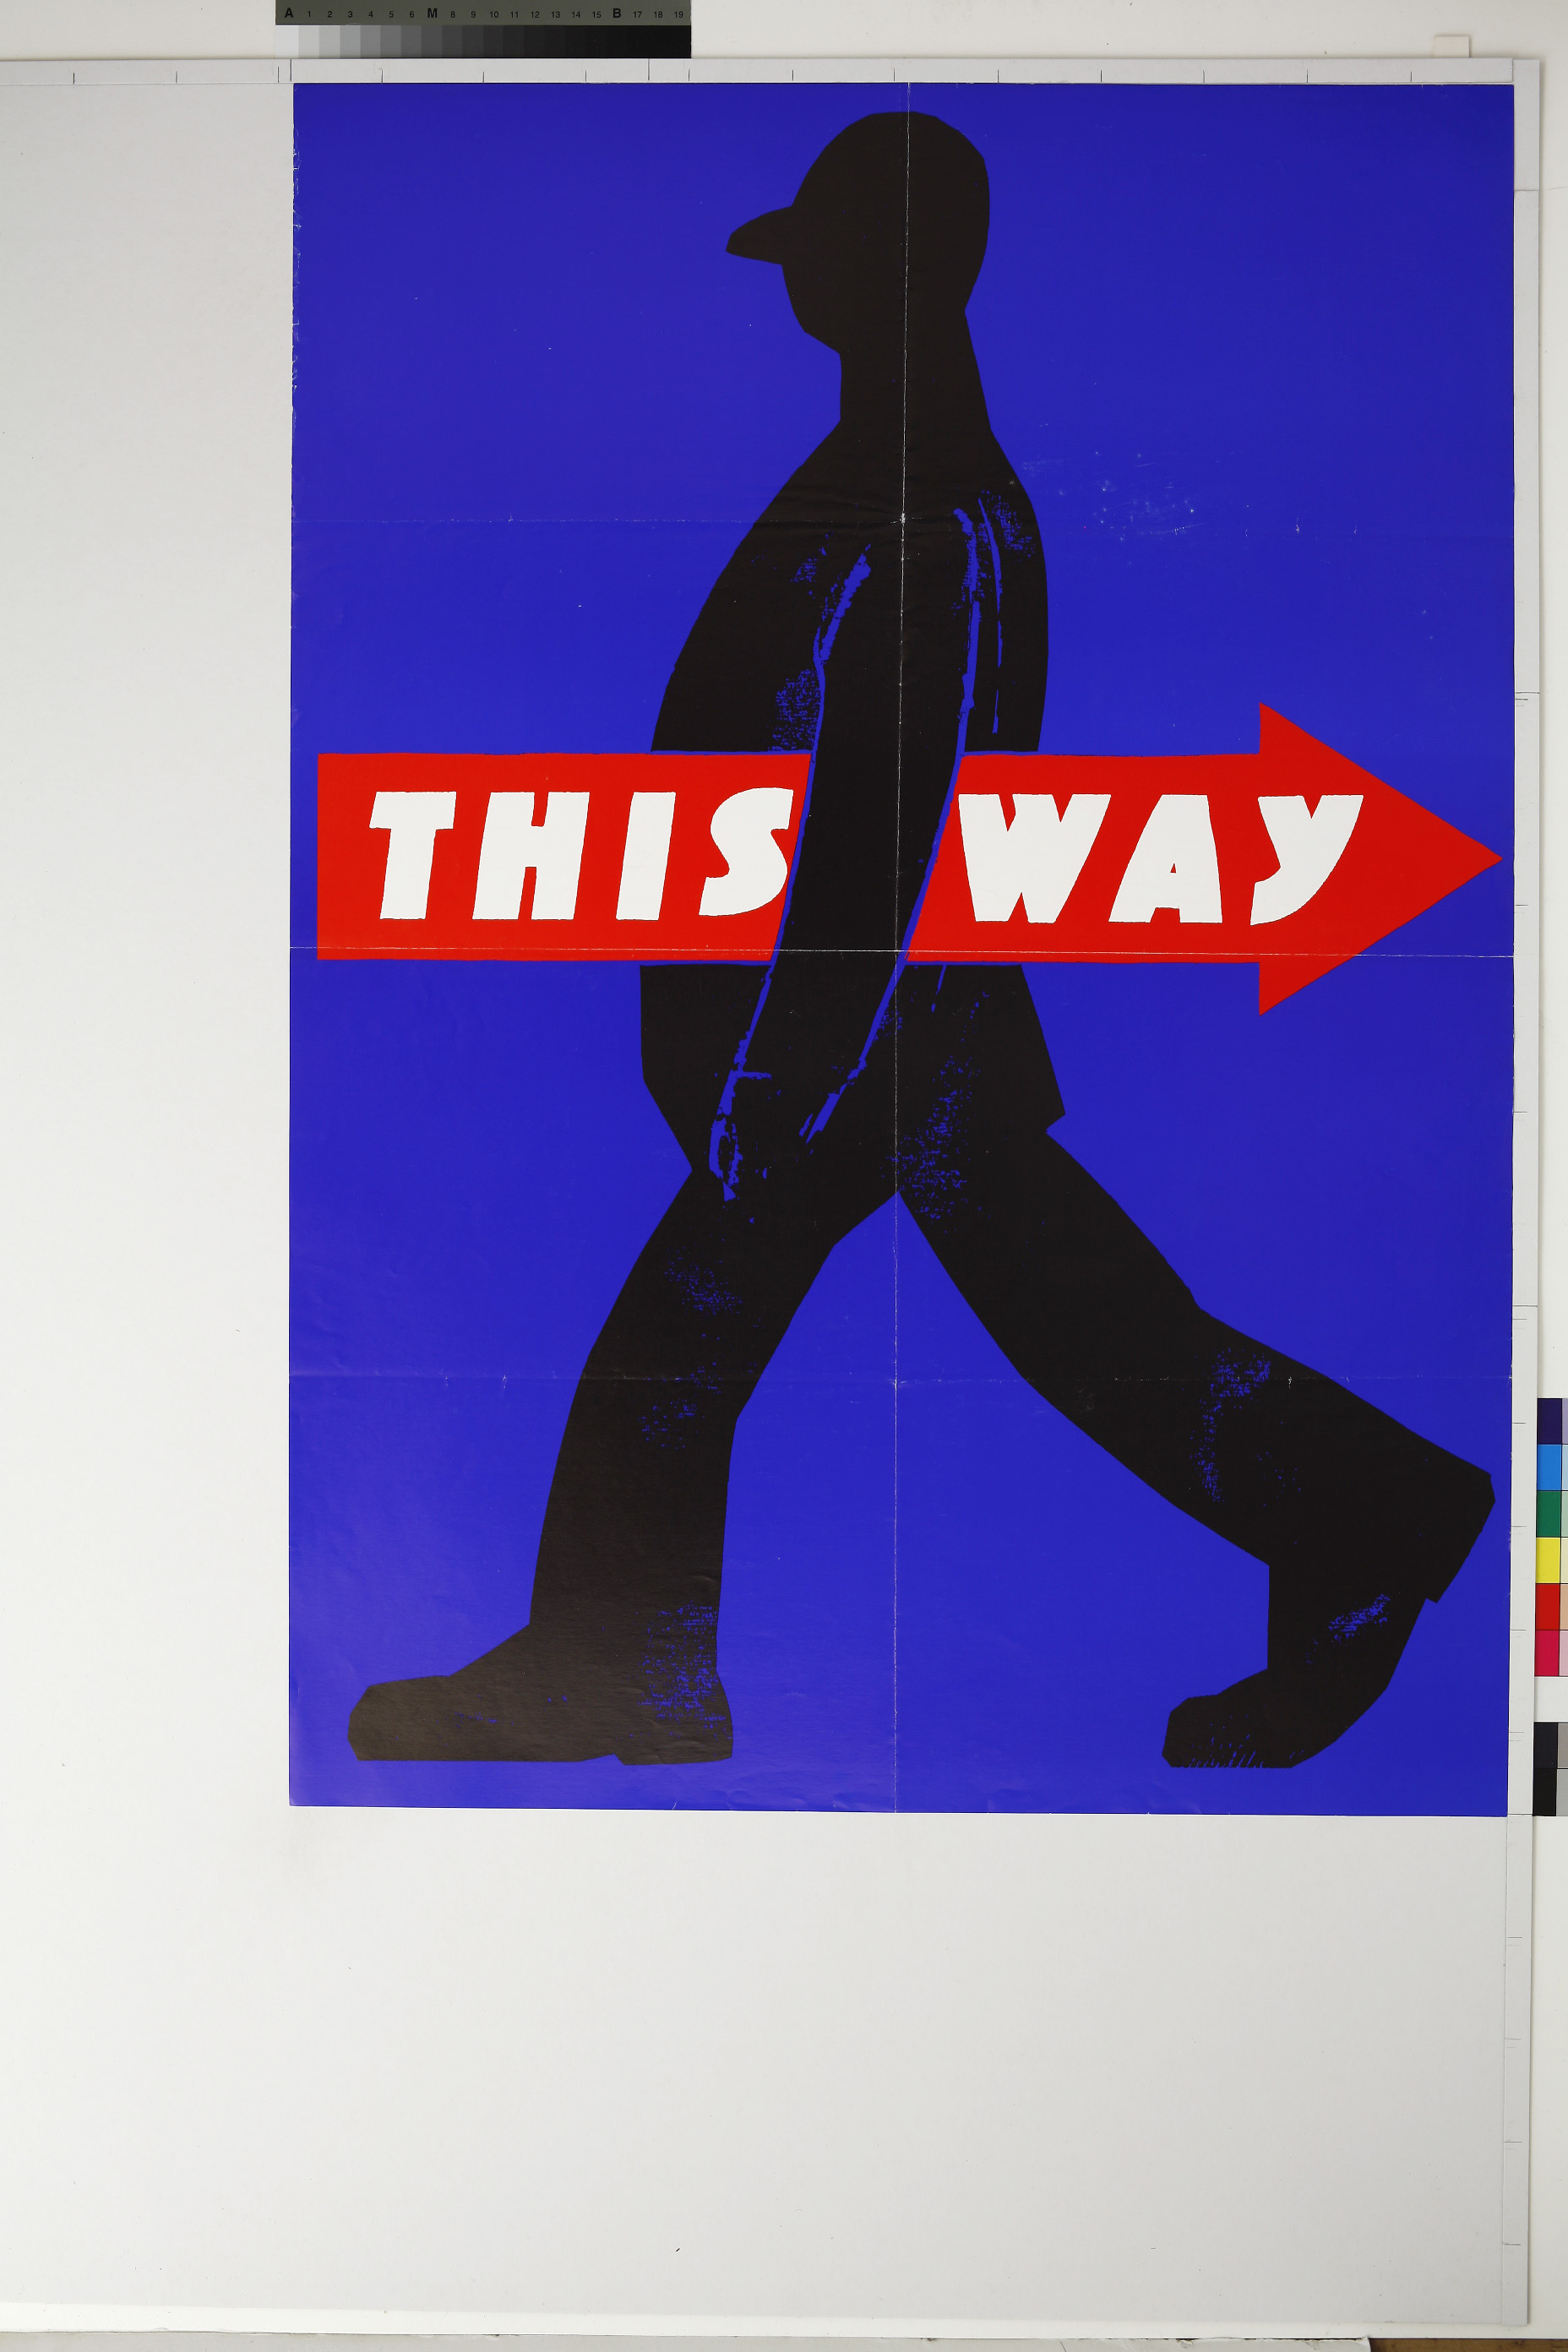
\includegraphics[width=\linewidth]{Abbildung_15_(vierzehn3_036)}
\centering
\caption{Plakat mit geringem Informationsgehalt (vierzehn3\_036).}
\end{figure}

\newpage
\begin{figure}[ht]
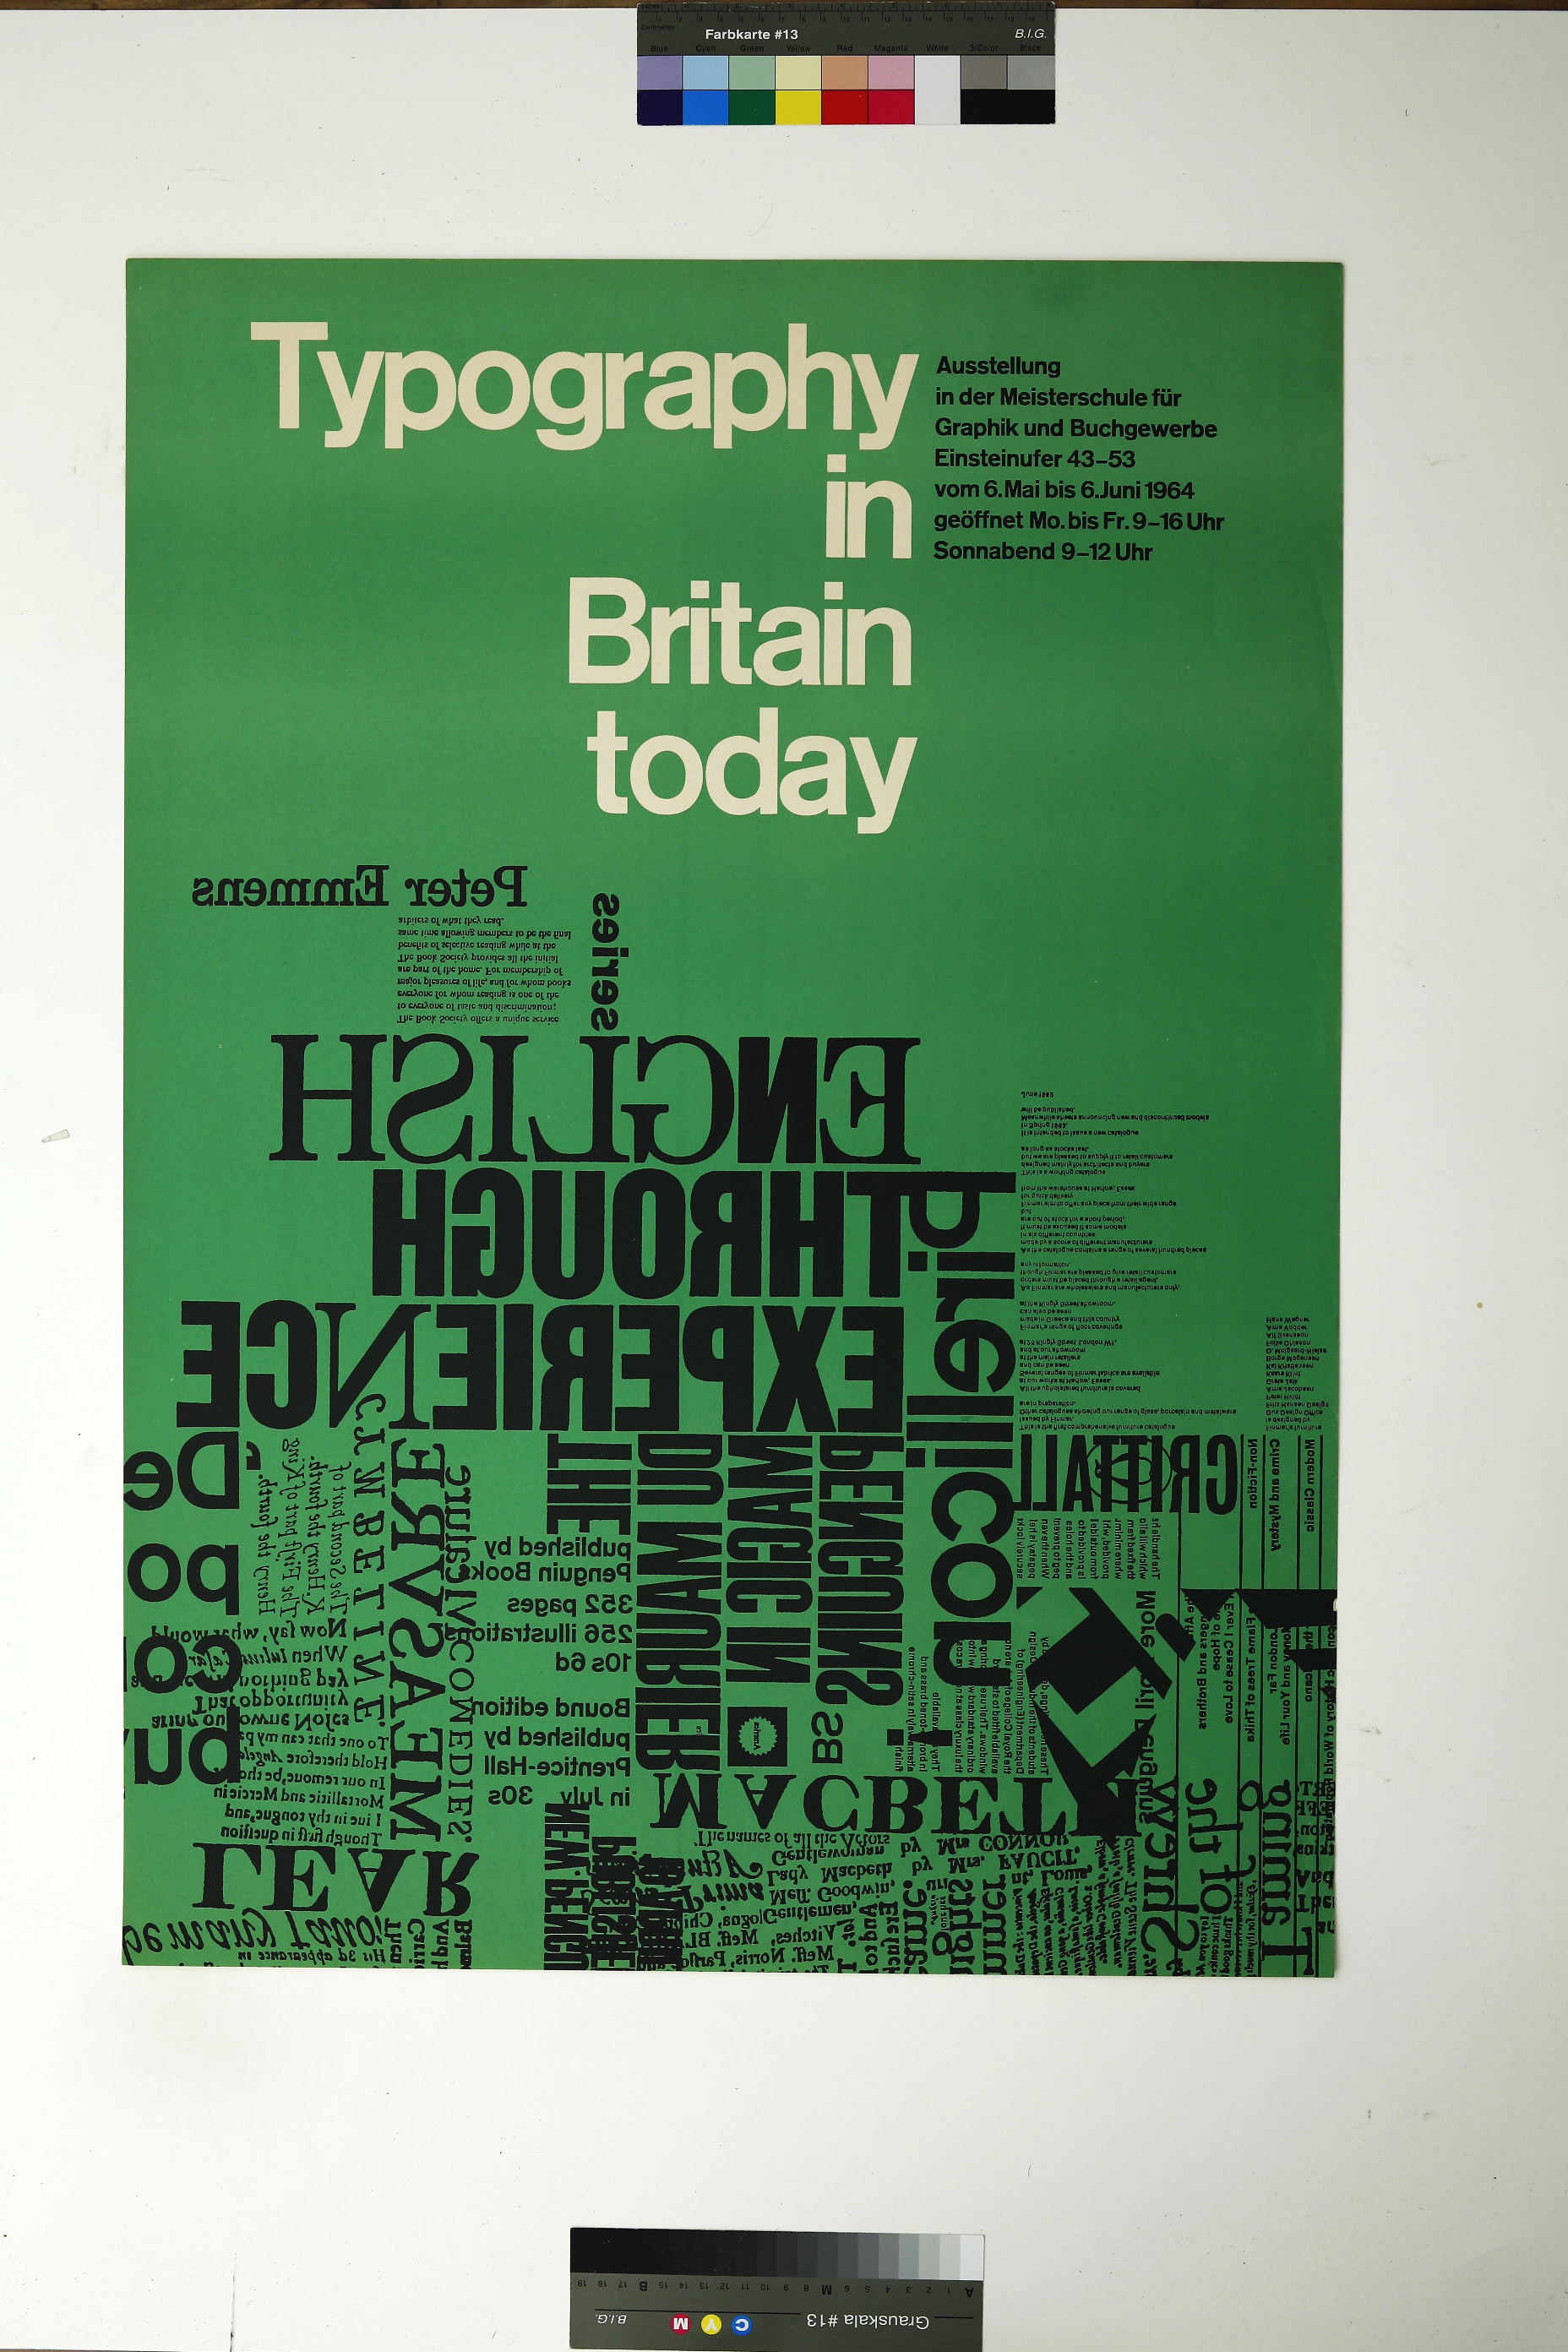
\includegraphics[width=\linewidth]{Abbildung_16_(acht2_081)}
\centering
\caption{Ausstellungsplakat – Topography in Britain Today, Meisterschule für Graphik und Buchgewerbe, 06.05.1964-06.06.1964 (acht2\_081).}
\end{figure}

\newpage
\begin{landscape}
\begin{figure}[ht]
	\begin{subfigure}[b]{0.5\linewidth}
	\centering
	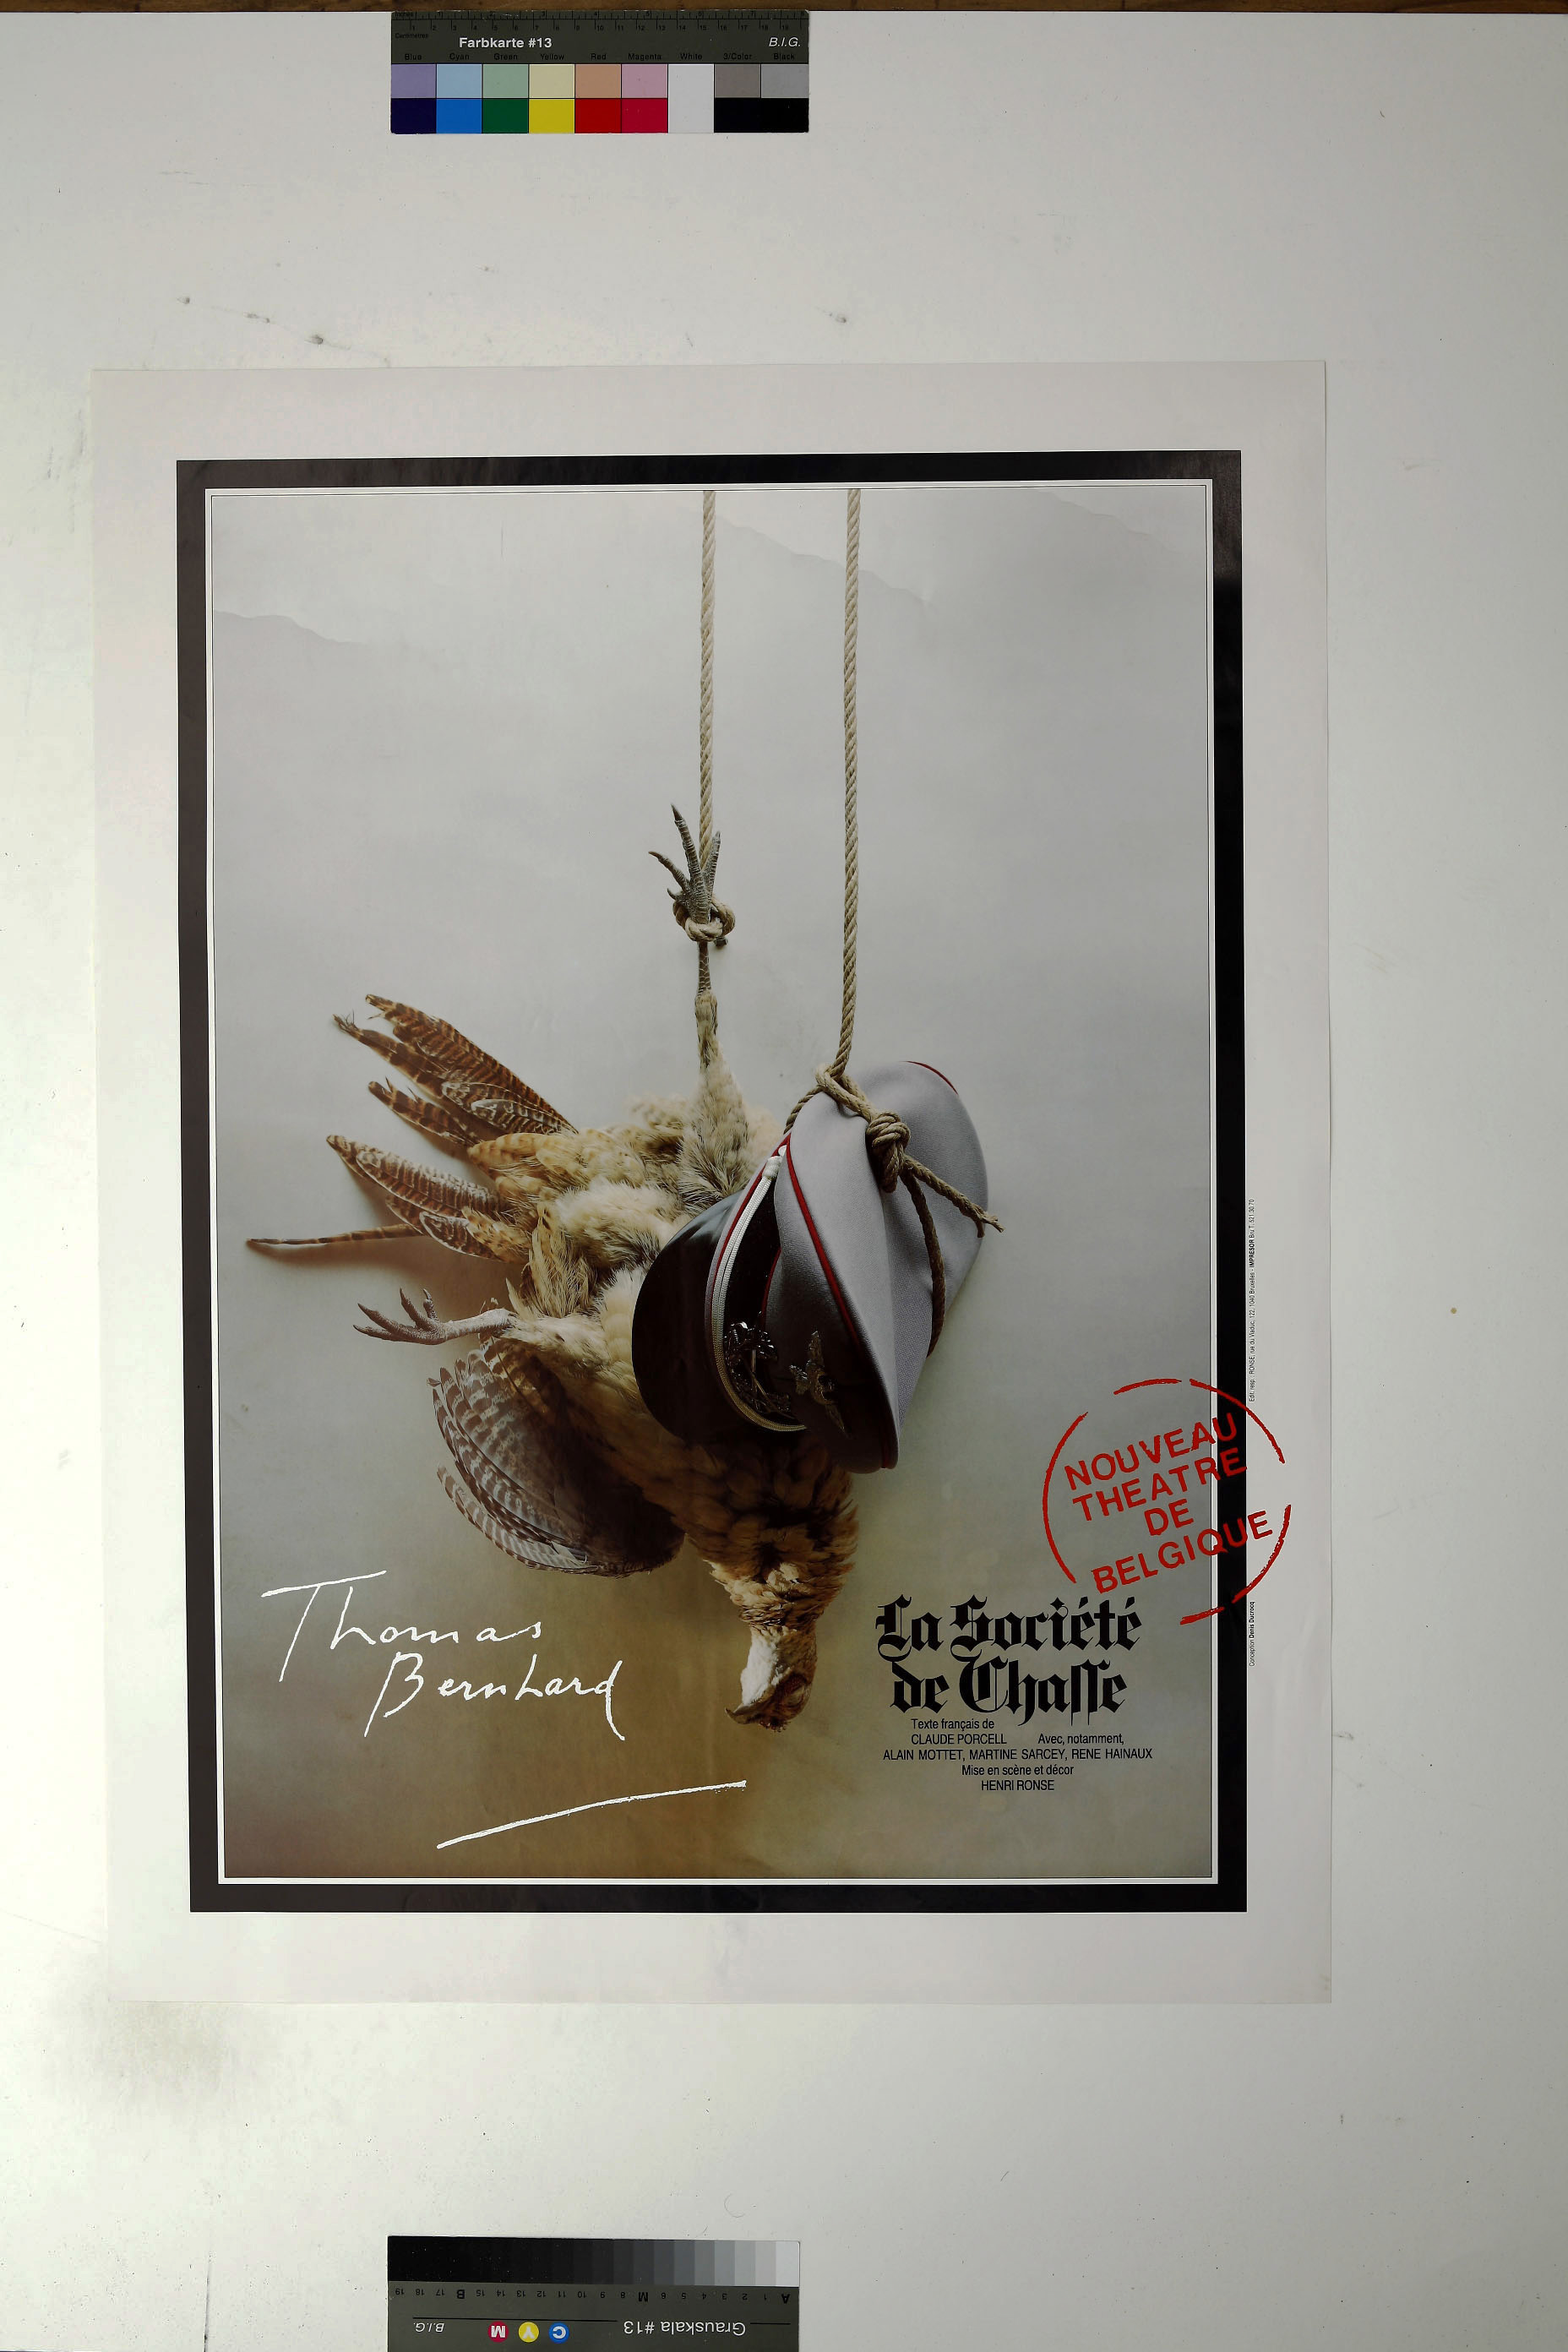
\includegraphics[height=\linewidth]{Abbildung_17_(acht1_006)}
	\end{subfigure}
	\begin{subfigure}[b]{0.5\linewidth}
	\centering
	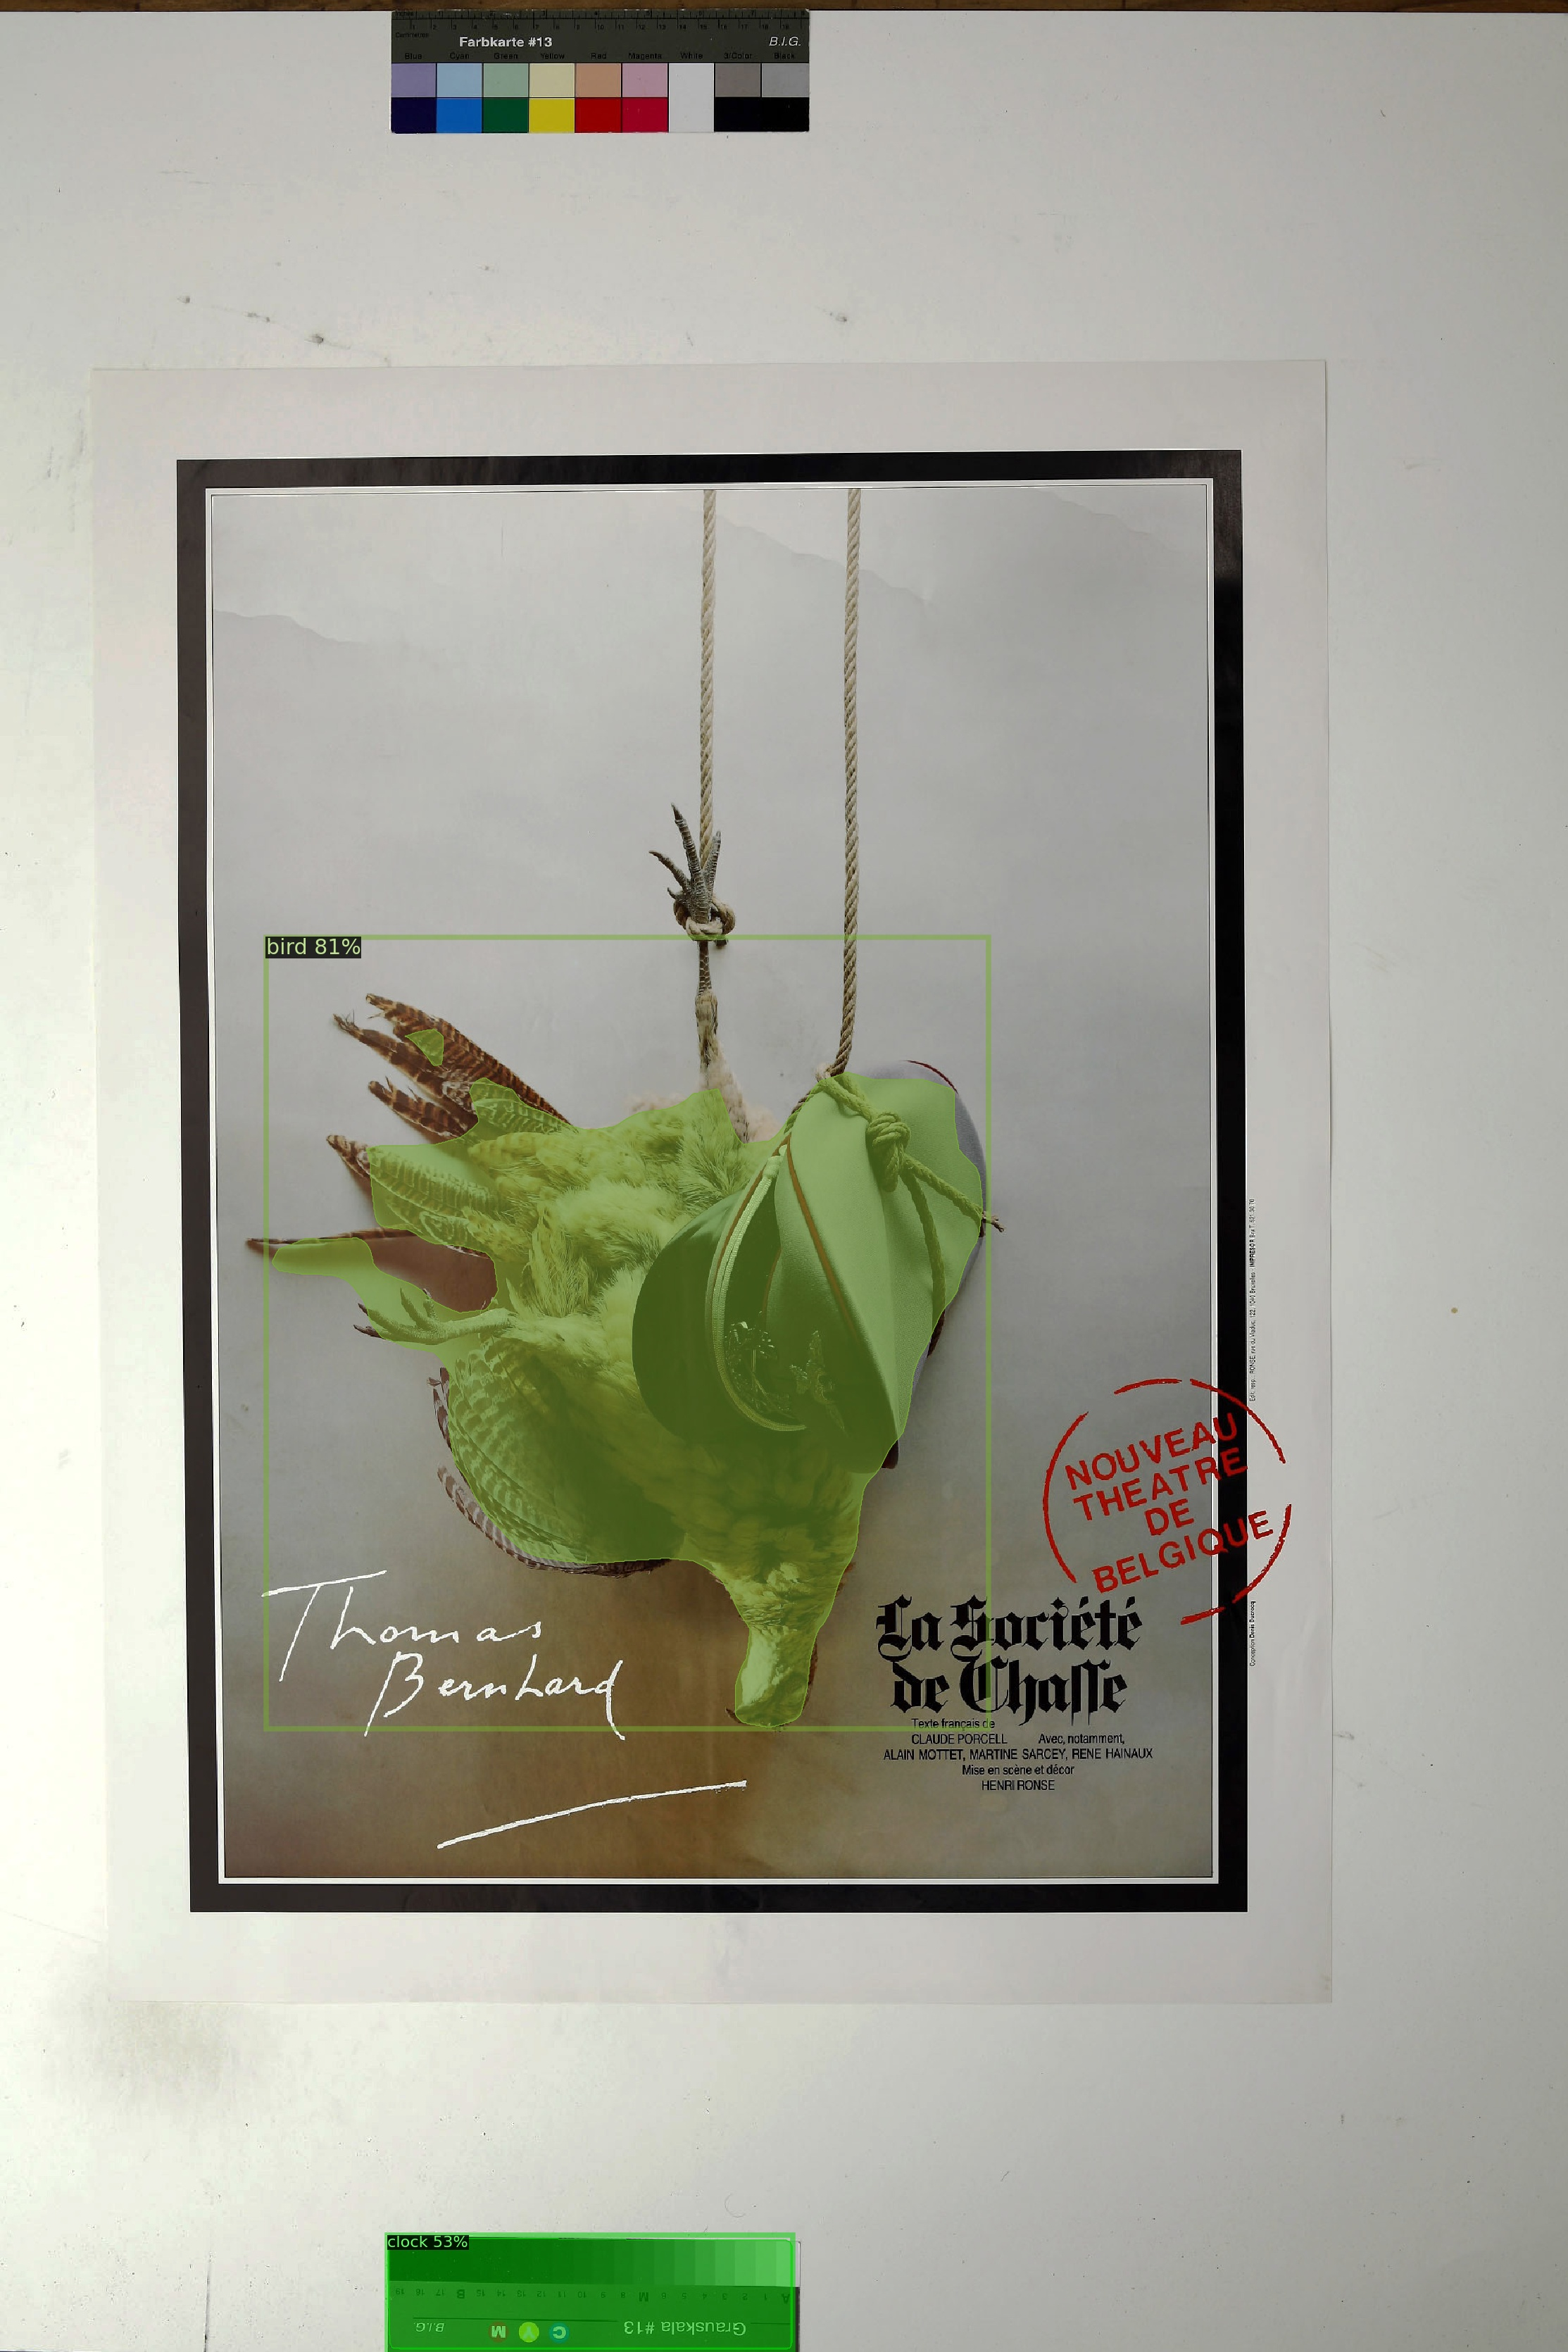
\includegraphics[height=\linewidth]{Abbildung_17_(acht1_006)_with_detections}
	\end{subfigure}
	\caption{Theaterplakat - La Société de Challe. Nouveau Theatre de Belgique, ohne Datum (acht1\_006); Rechts: Mit Annotationen.}
\end{figure}
\end{landscape}

\newpage
\begin{landscape}
\begin{figure}[ht]
	\begin{subfigure}[b]{0.5\linewidth}
	\centering
	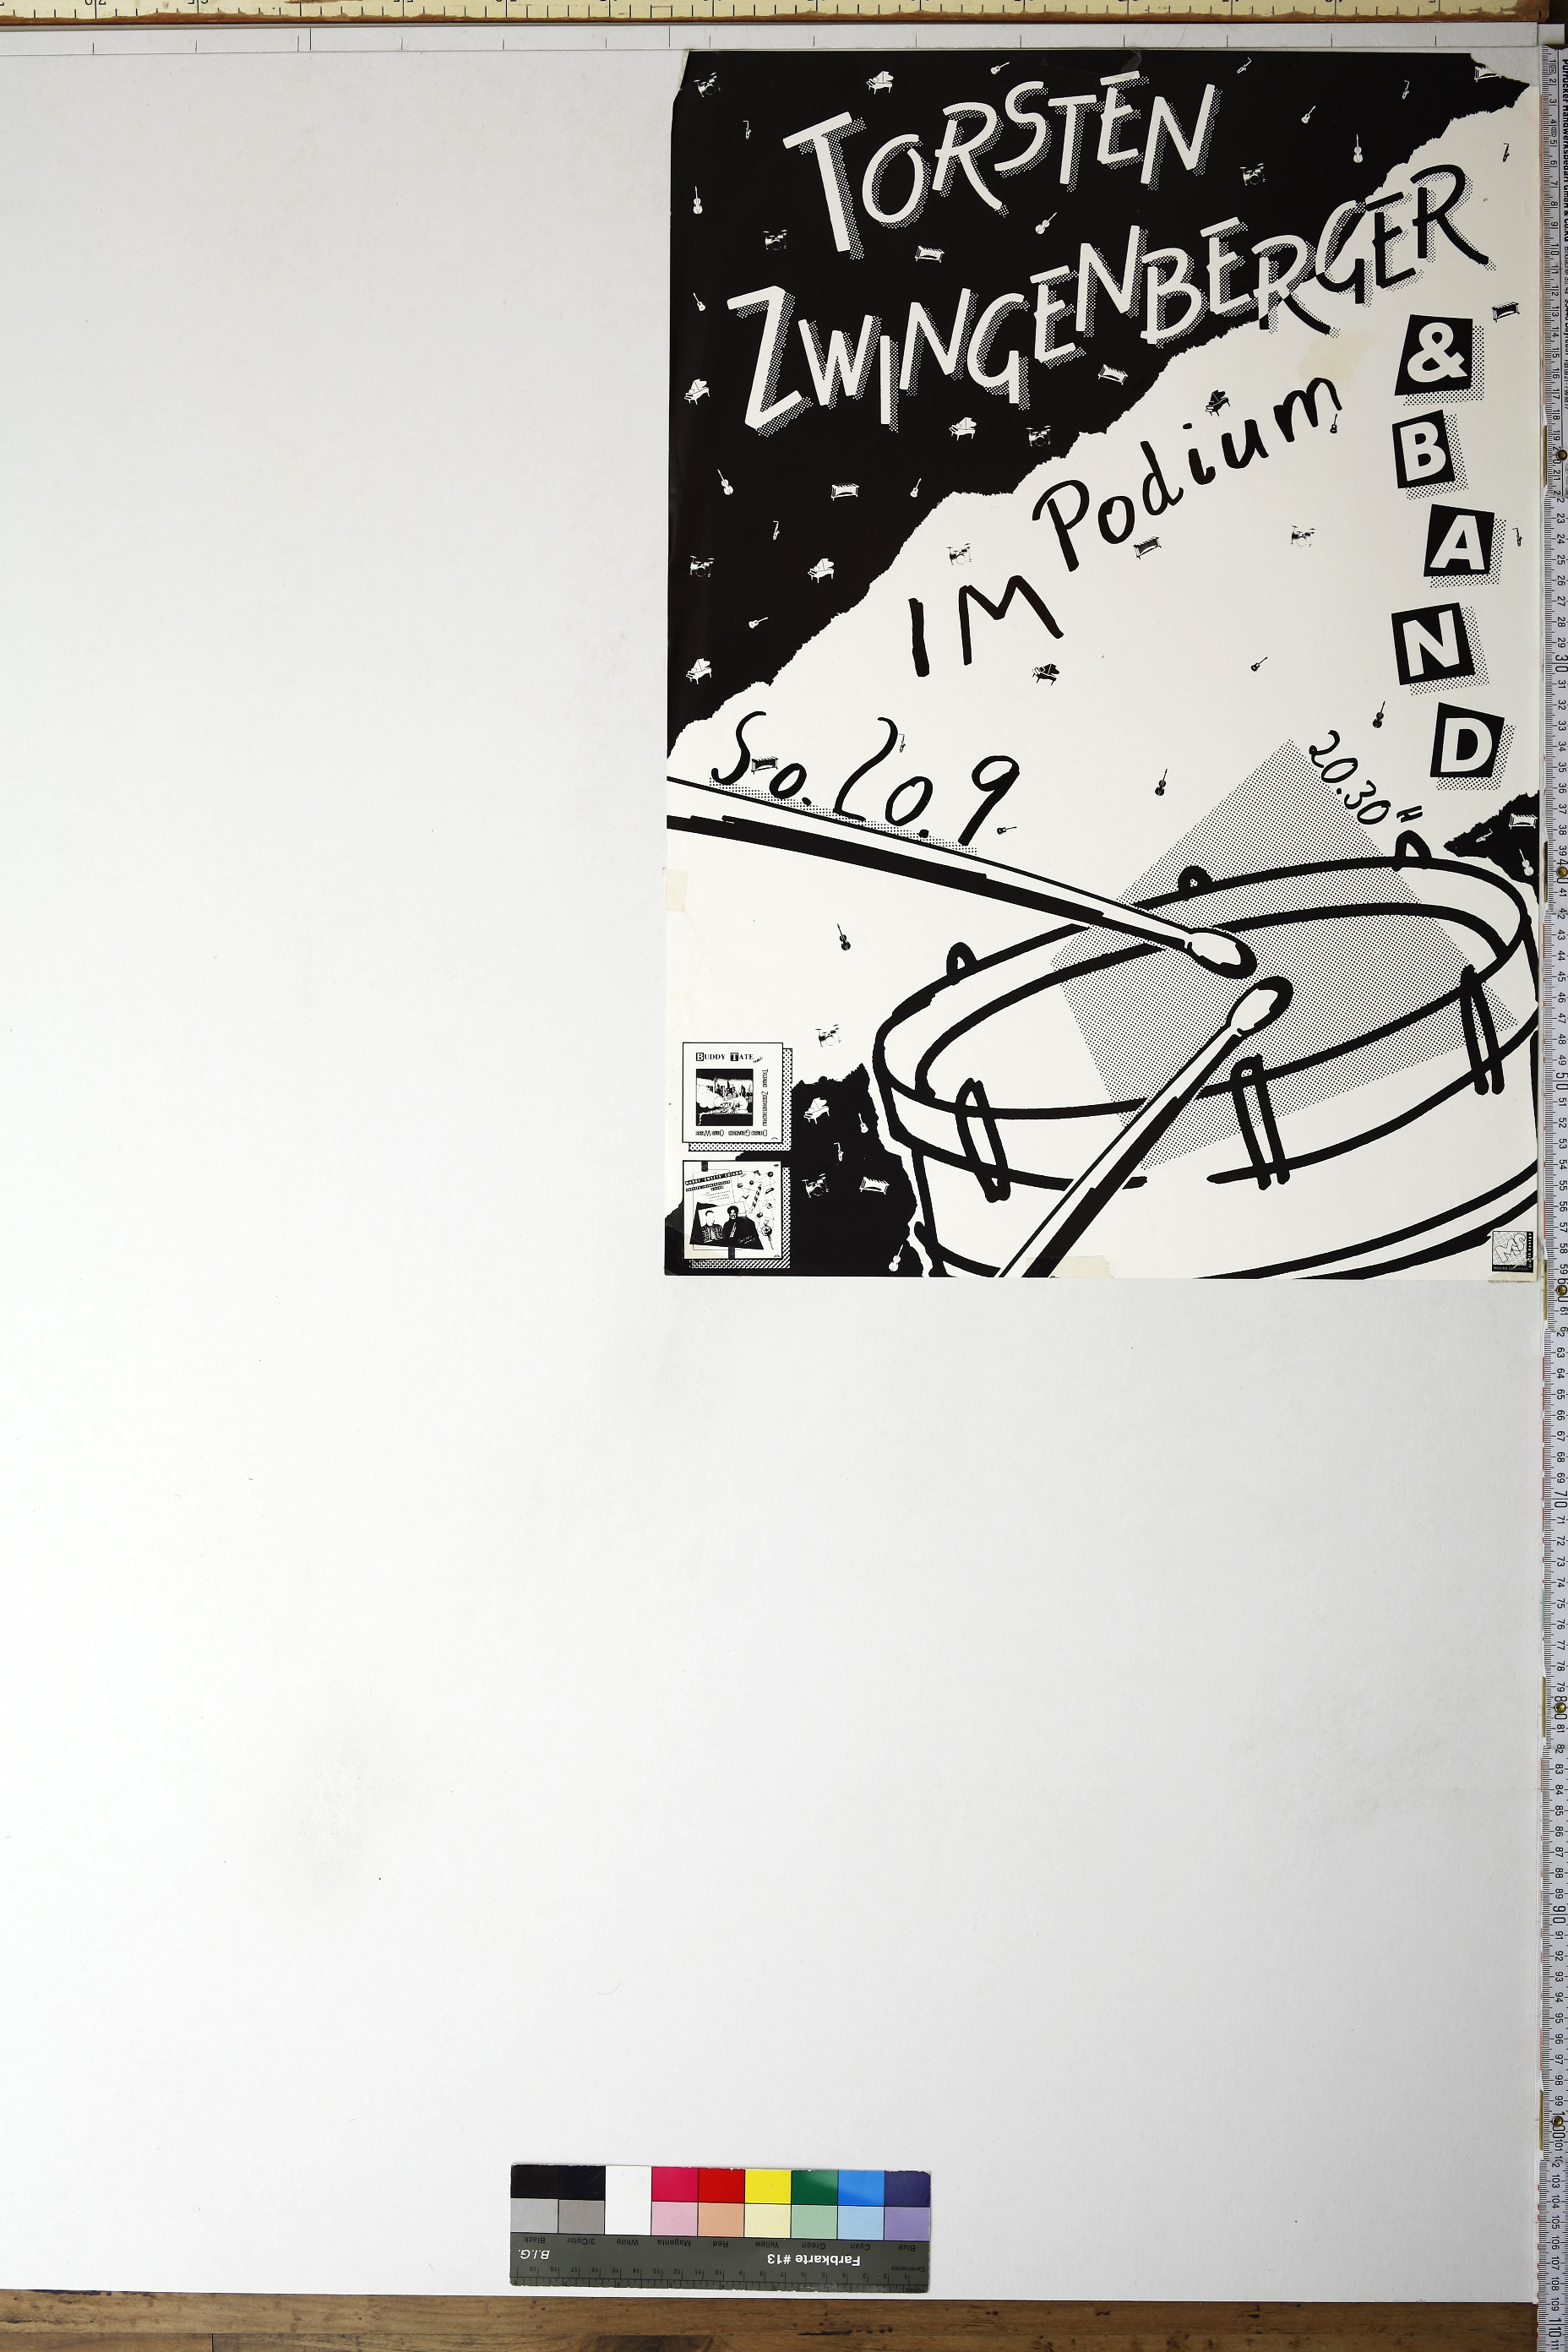
\includegraphics[height=\linewidth]{Abbildung_18_(acht4_096)}
	\end{subfigure}
	\begin{subfigure}[b]{0.5\linewidth}
	\centering
	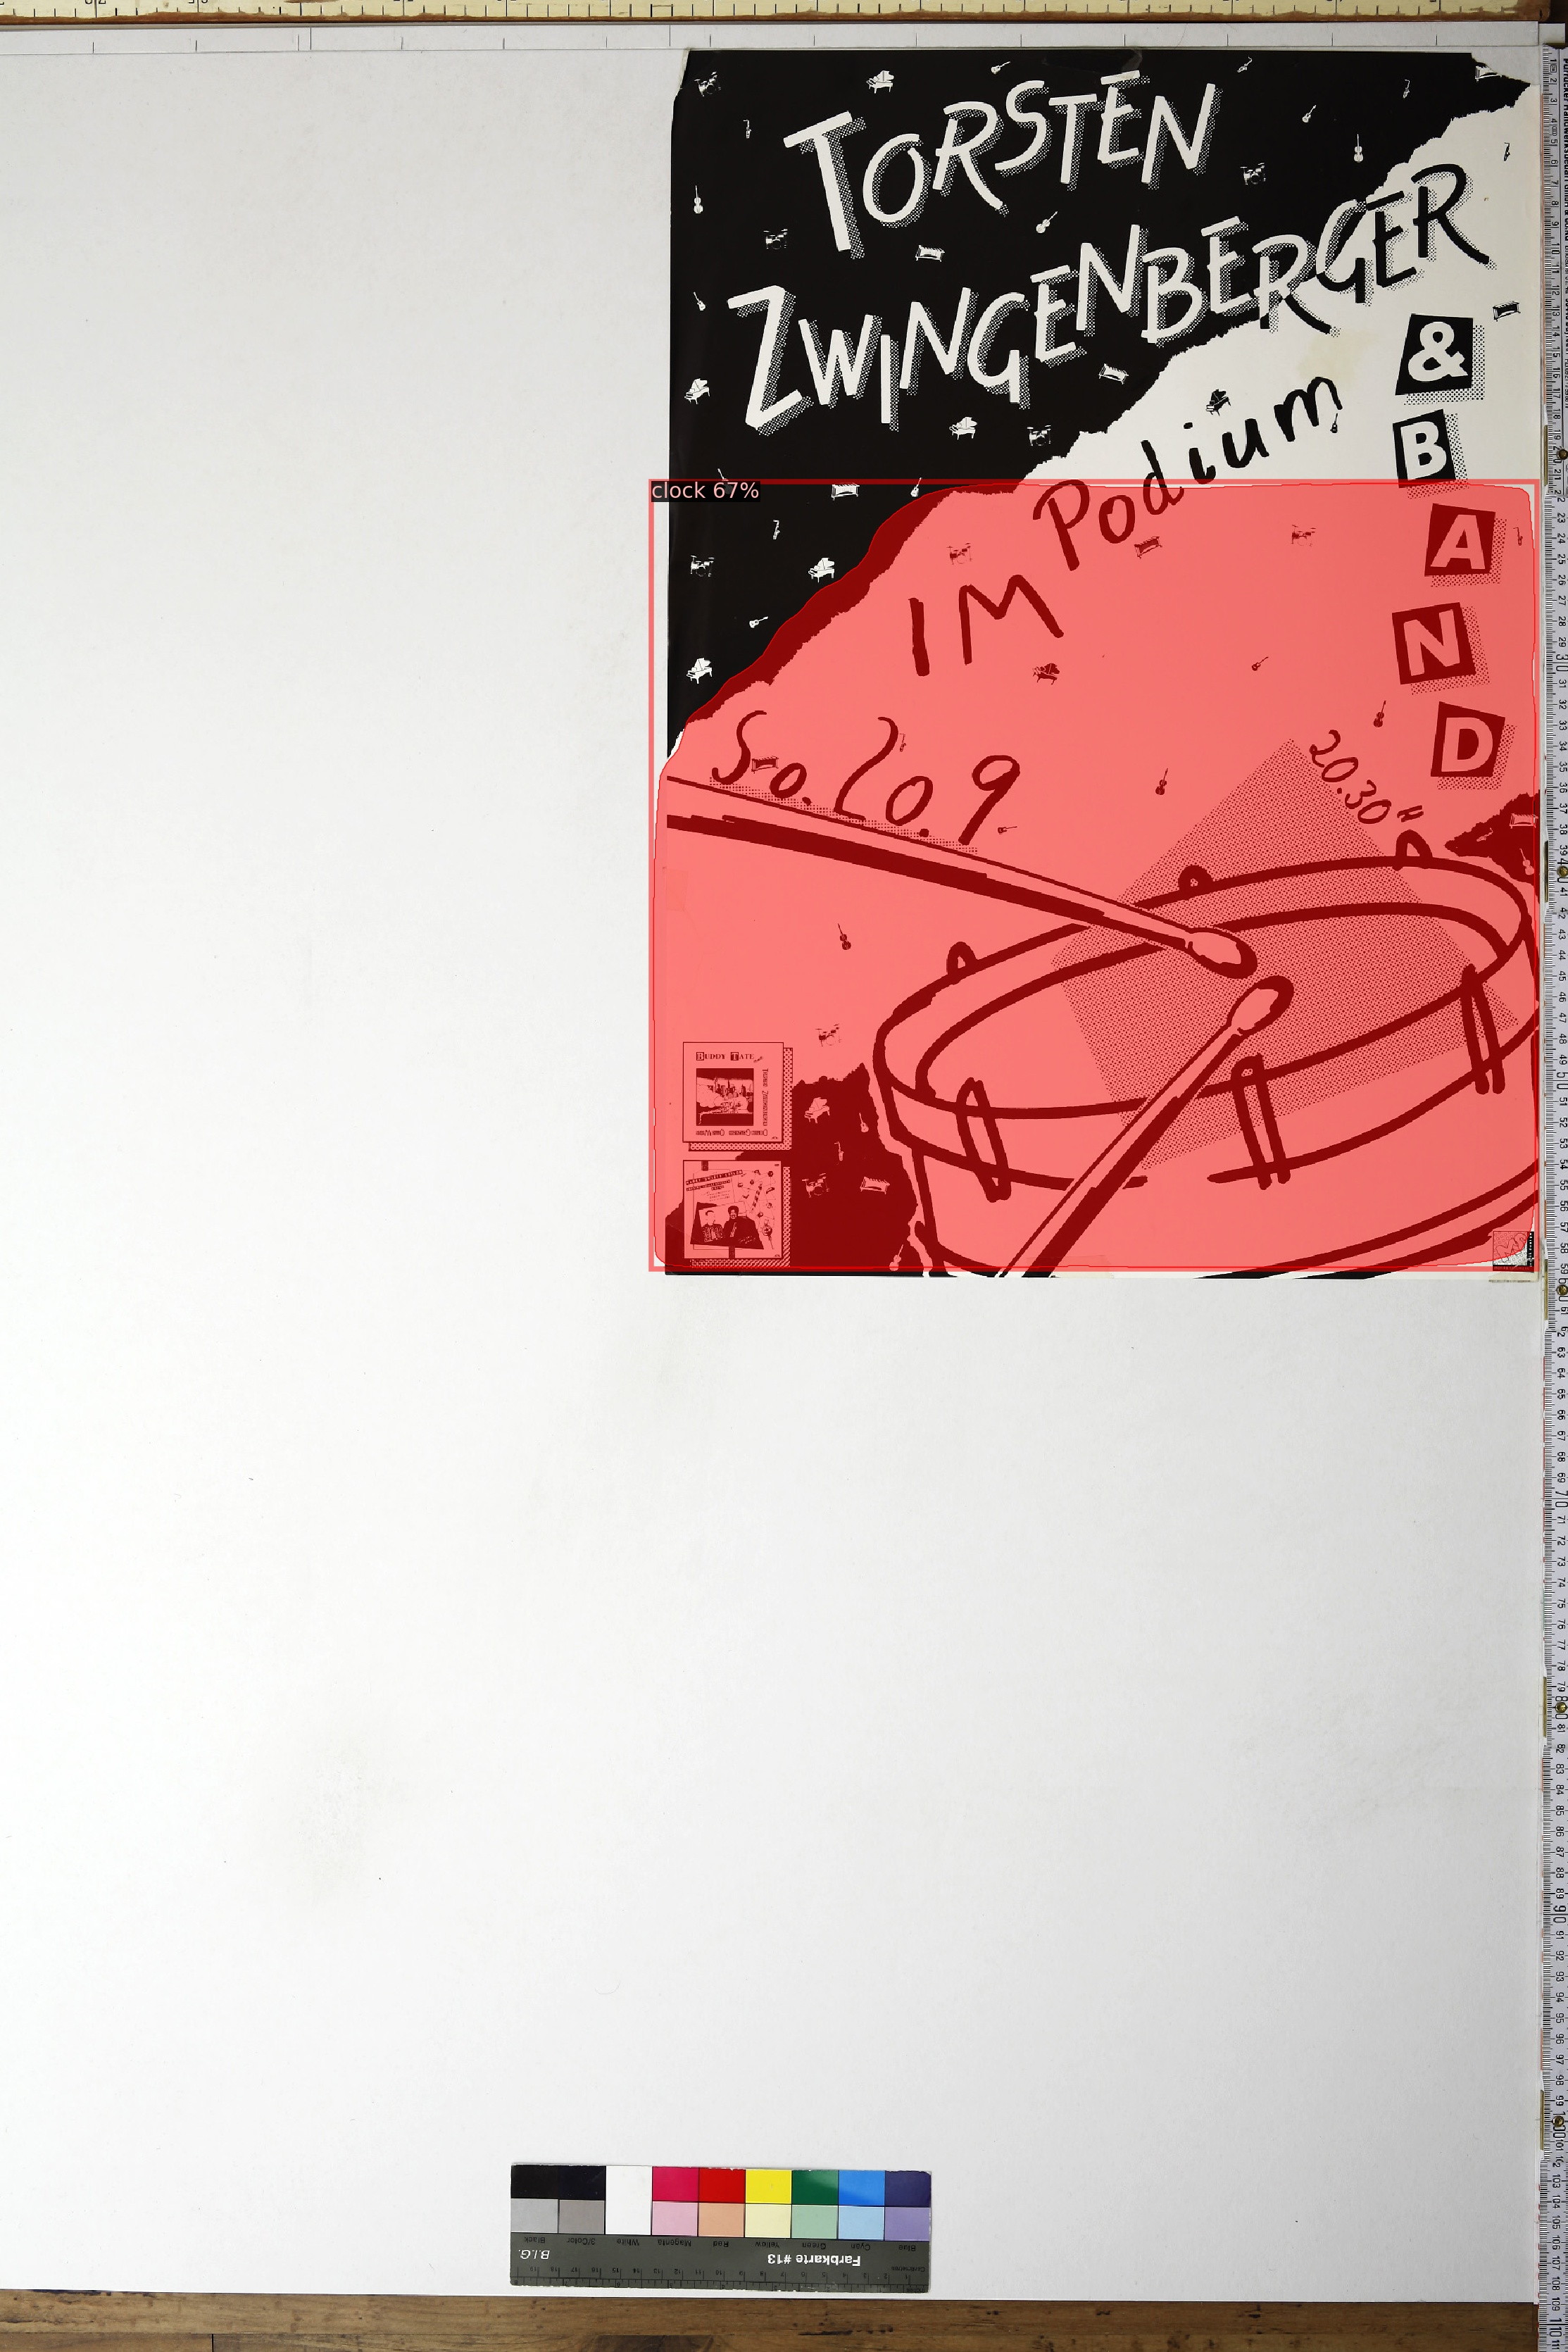
\includegraphics[height=\linewidth]{Abbildung_18_(acht4_096)_with_detections}
	\end{subfigure}
	\caption{Veranstaltungsplakat – Torsten Zwingenberger im Podium \& Band, 20.09 (acht4\_096); Rechts: Mit Annotationen.}
\end{figure}
\end{landscape}

\newpage
\begin{figure}[ht]
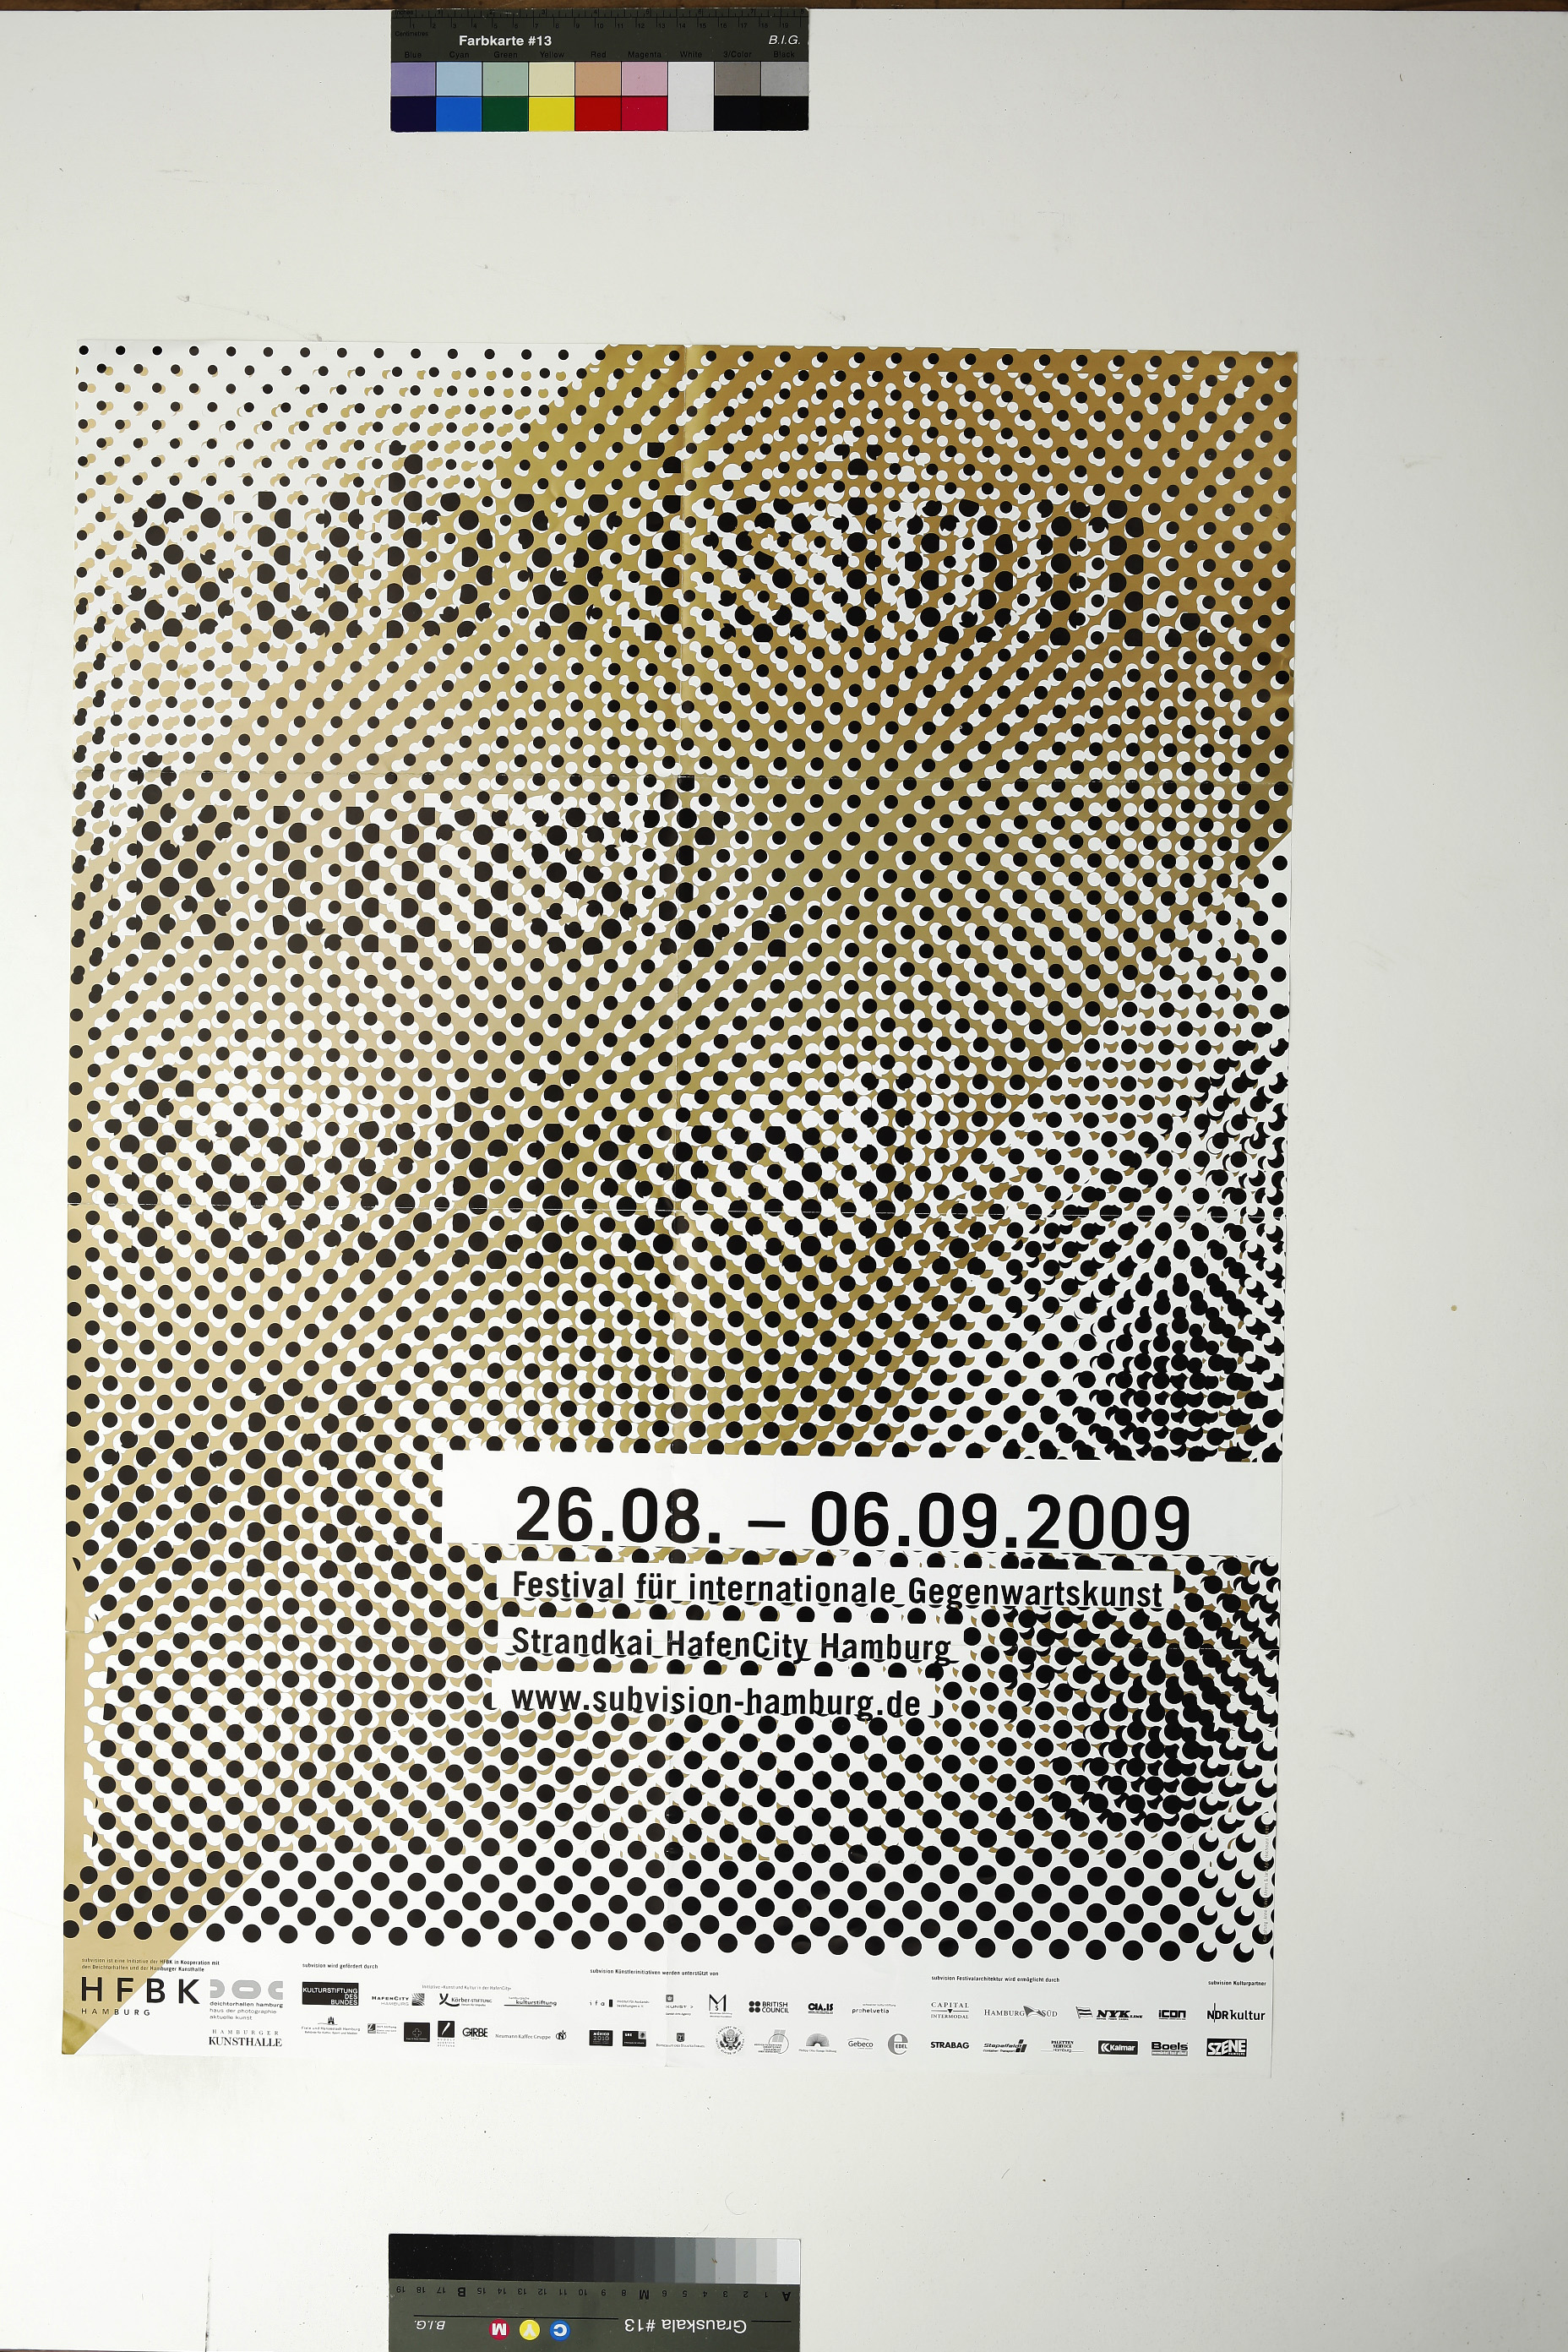
\includegraphics[width=\linewidth]{Abbildung_19_(acht1_131)}
\centering
\caption{Veranstaltungsplakat – Festival für internationale Gegenwartskunst, HFBK Hamburg, 26.08.2009-06.09.2009 (acht1\_131).}
\end{figure}

\newpage
\begin{figure}[ht]
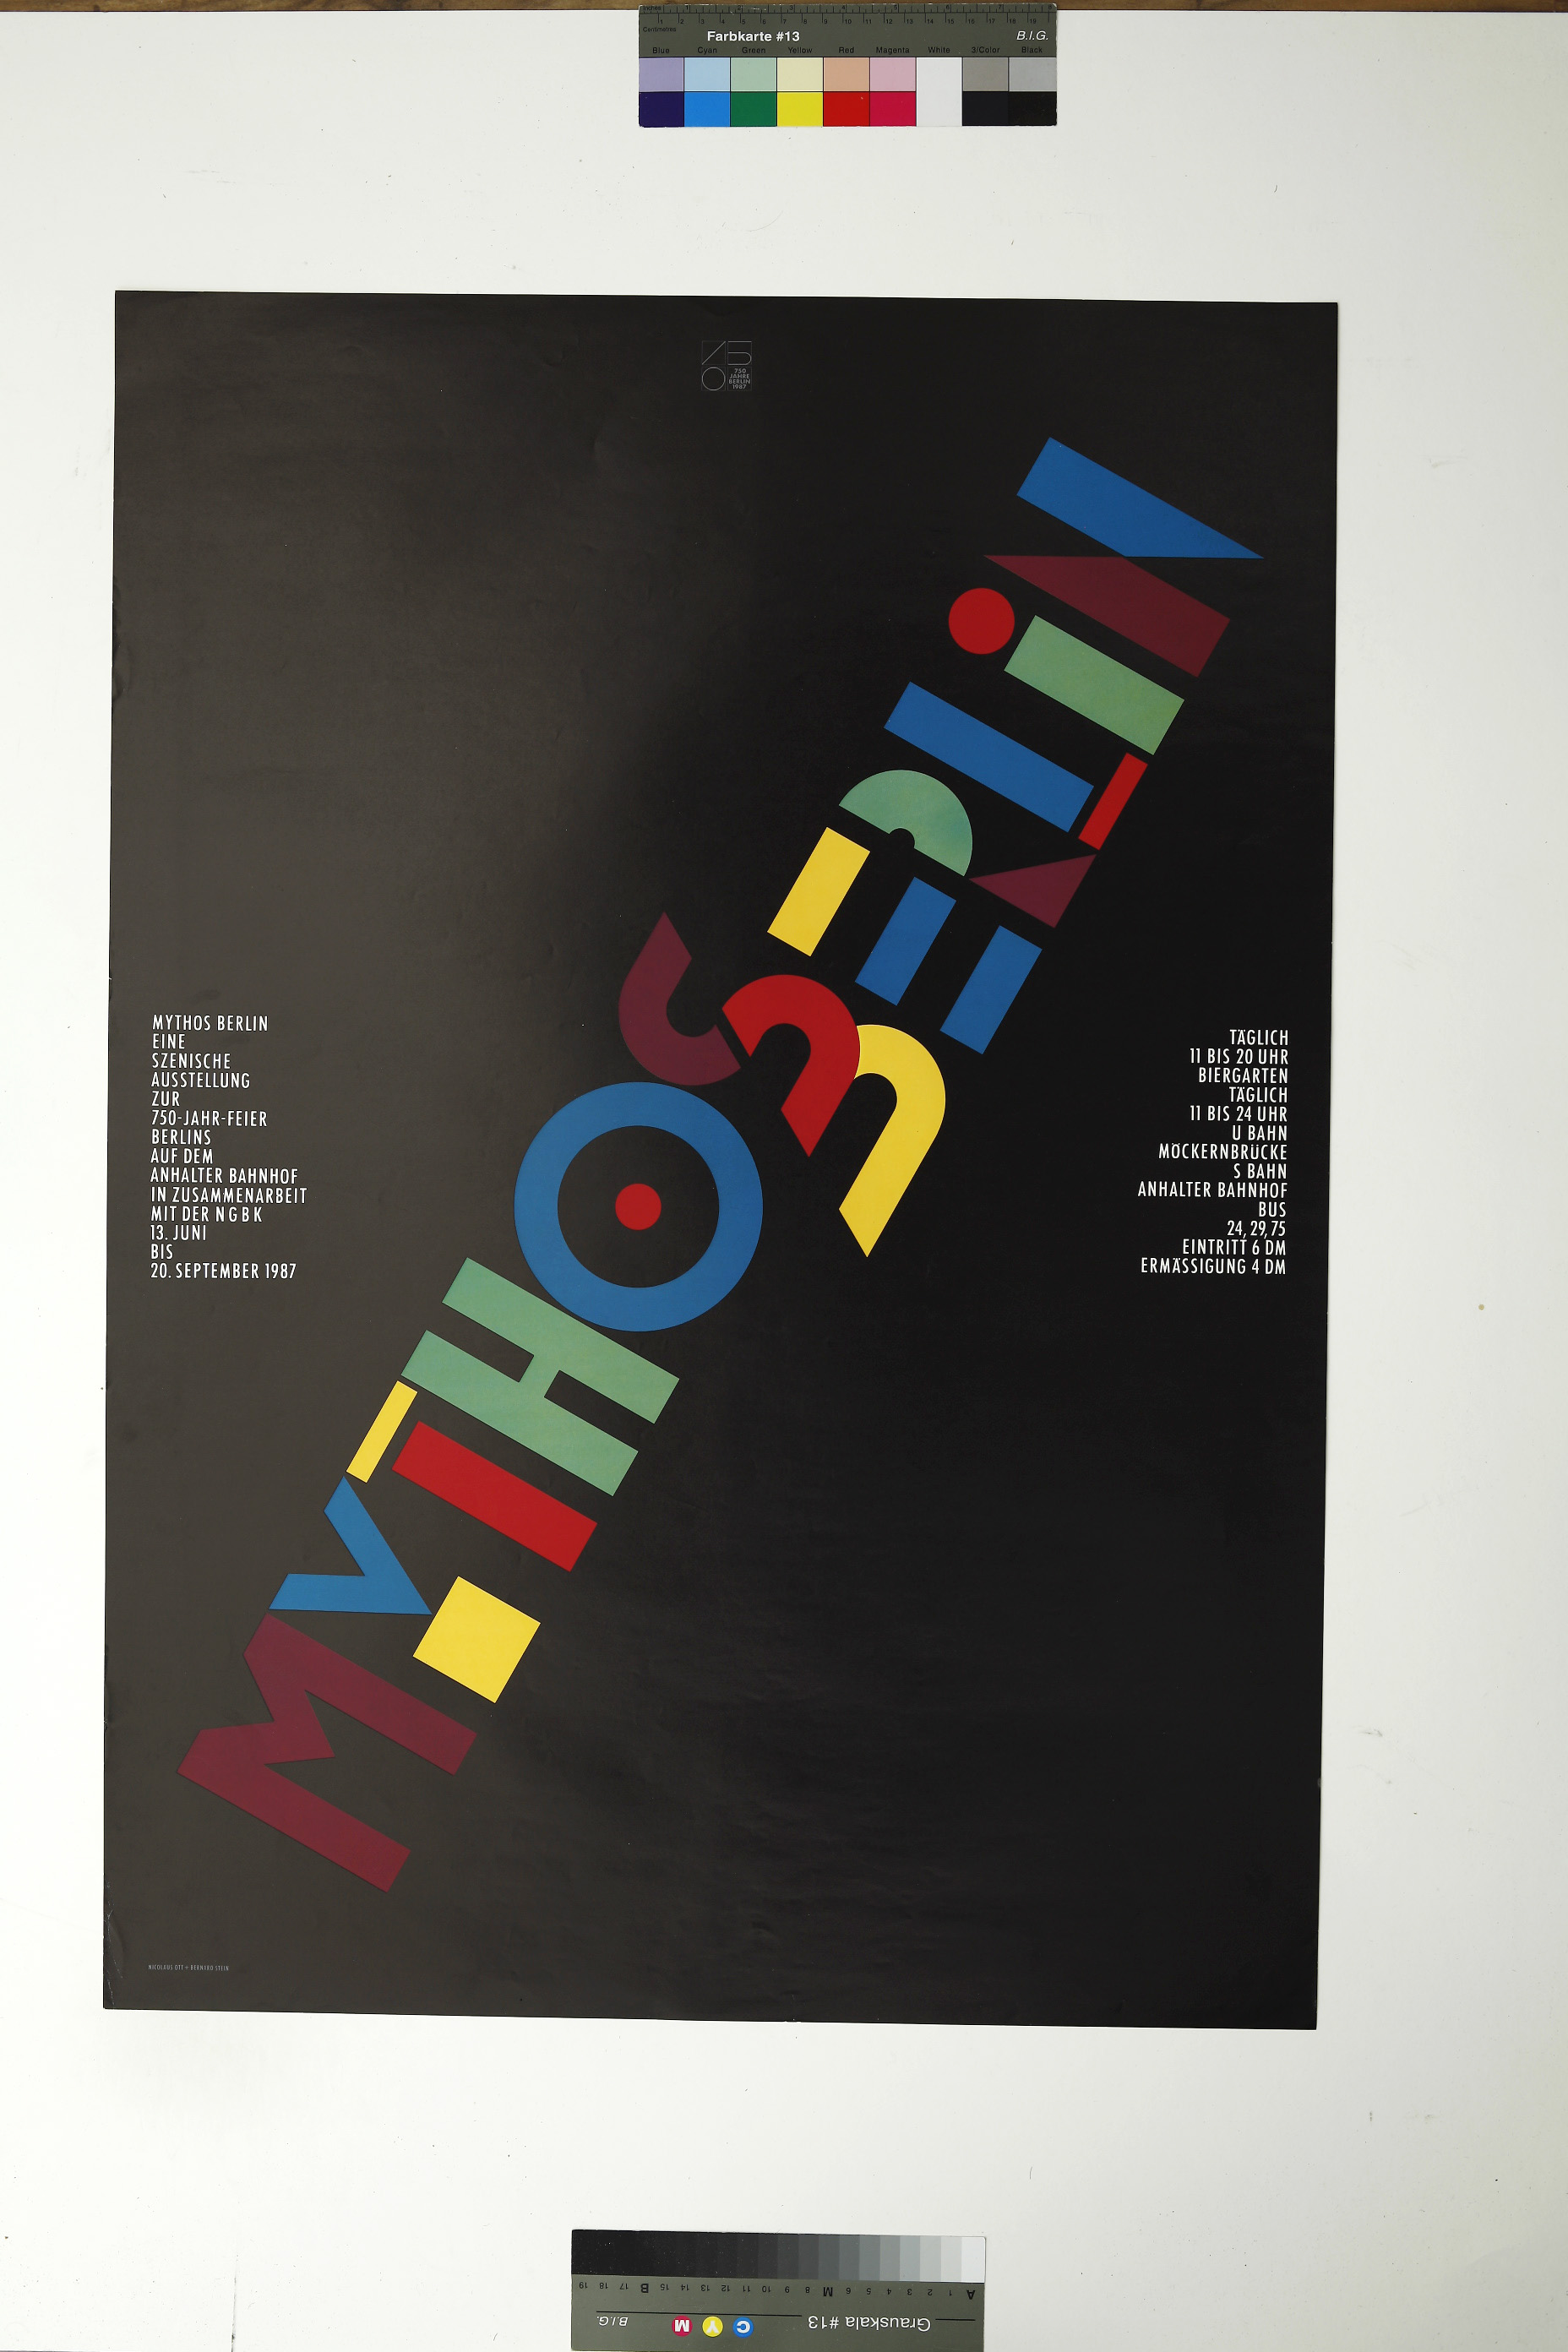
\includegraphics[width=\linewidth]{Abbildung_20_(acht2_049)}
\centering
\caption{Ausstellungsplakat – Mythos Berlin, Anhalter Bahnhof, 13.06.1987-20.09.1987 (acht2\_049).}
\end{figure}

\newpage
\begin{landscape}
\begin{figure}[ht]
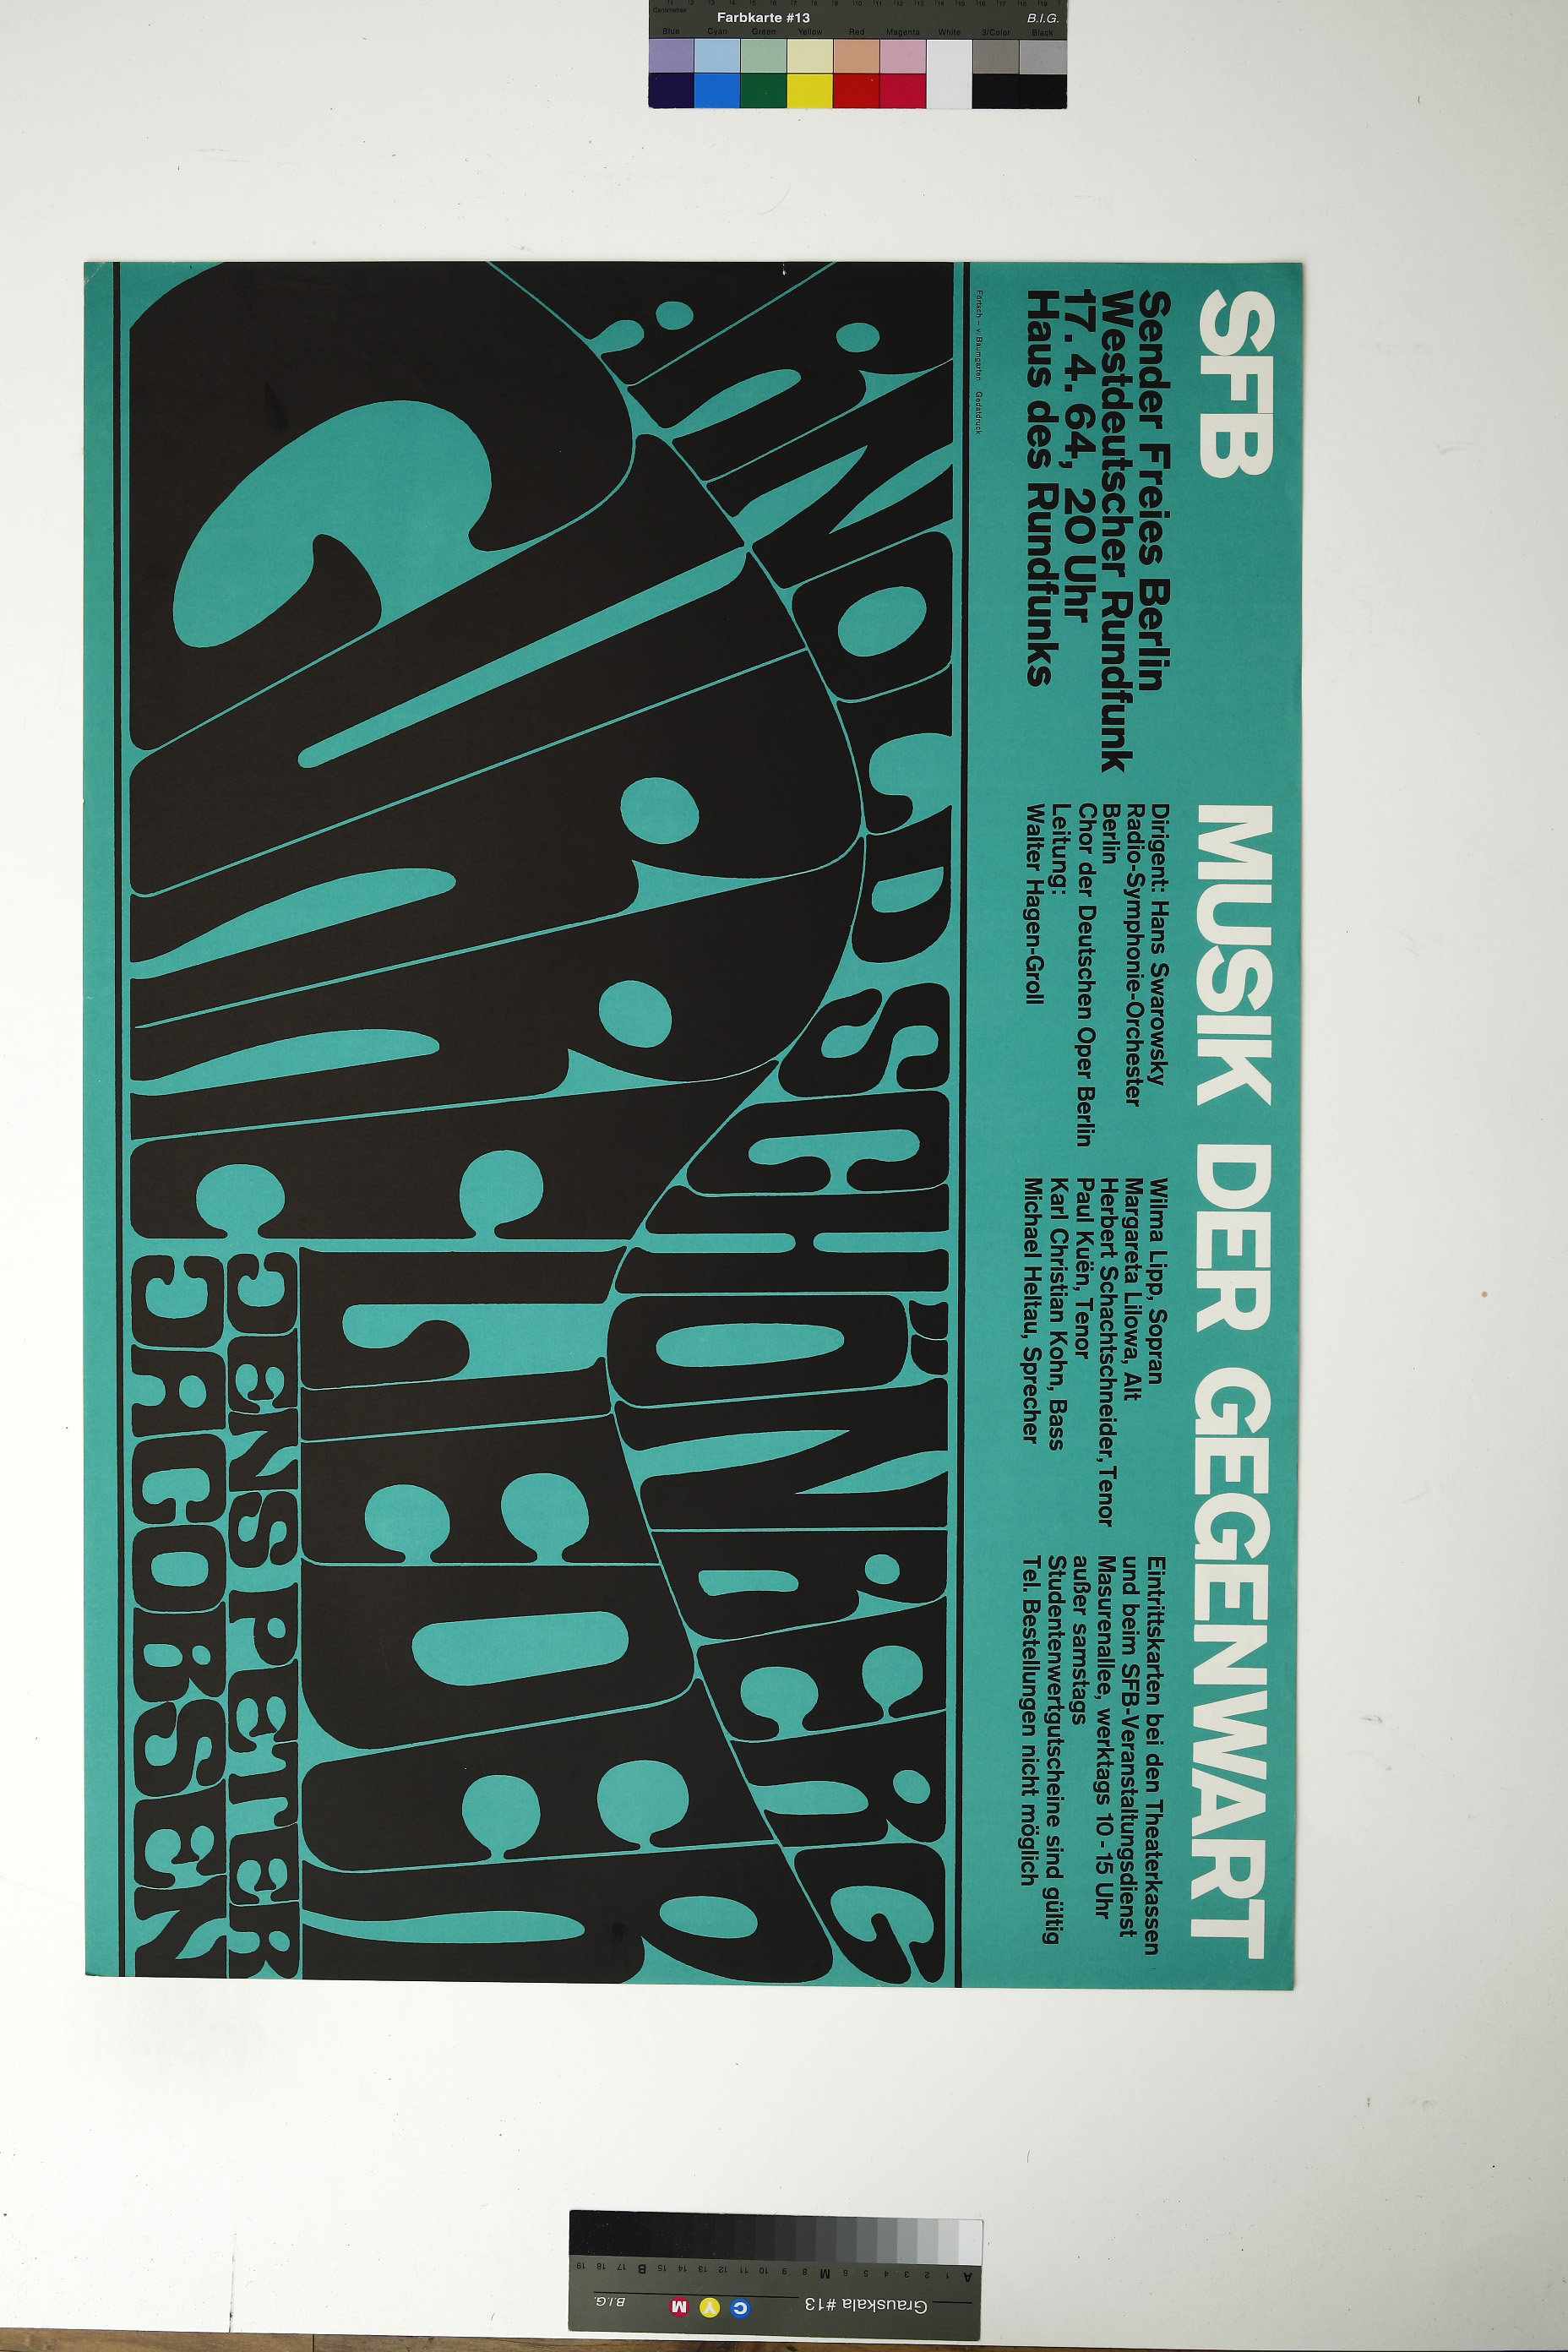
\includegraphics[height=0.85\linewidth, angle=90]{Abbildung_21_(acht2_112)}
\centering
\caption{Veranstaltungsplakat – Musik in der Gegenwart, Sender Freies Berlin, 17.04.1964 (acht2\_112).}
\end{figure}
\end{landscape}

\newpage
\begin{figure}[ht]
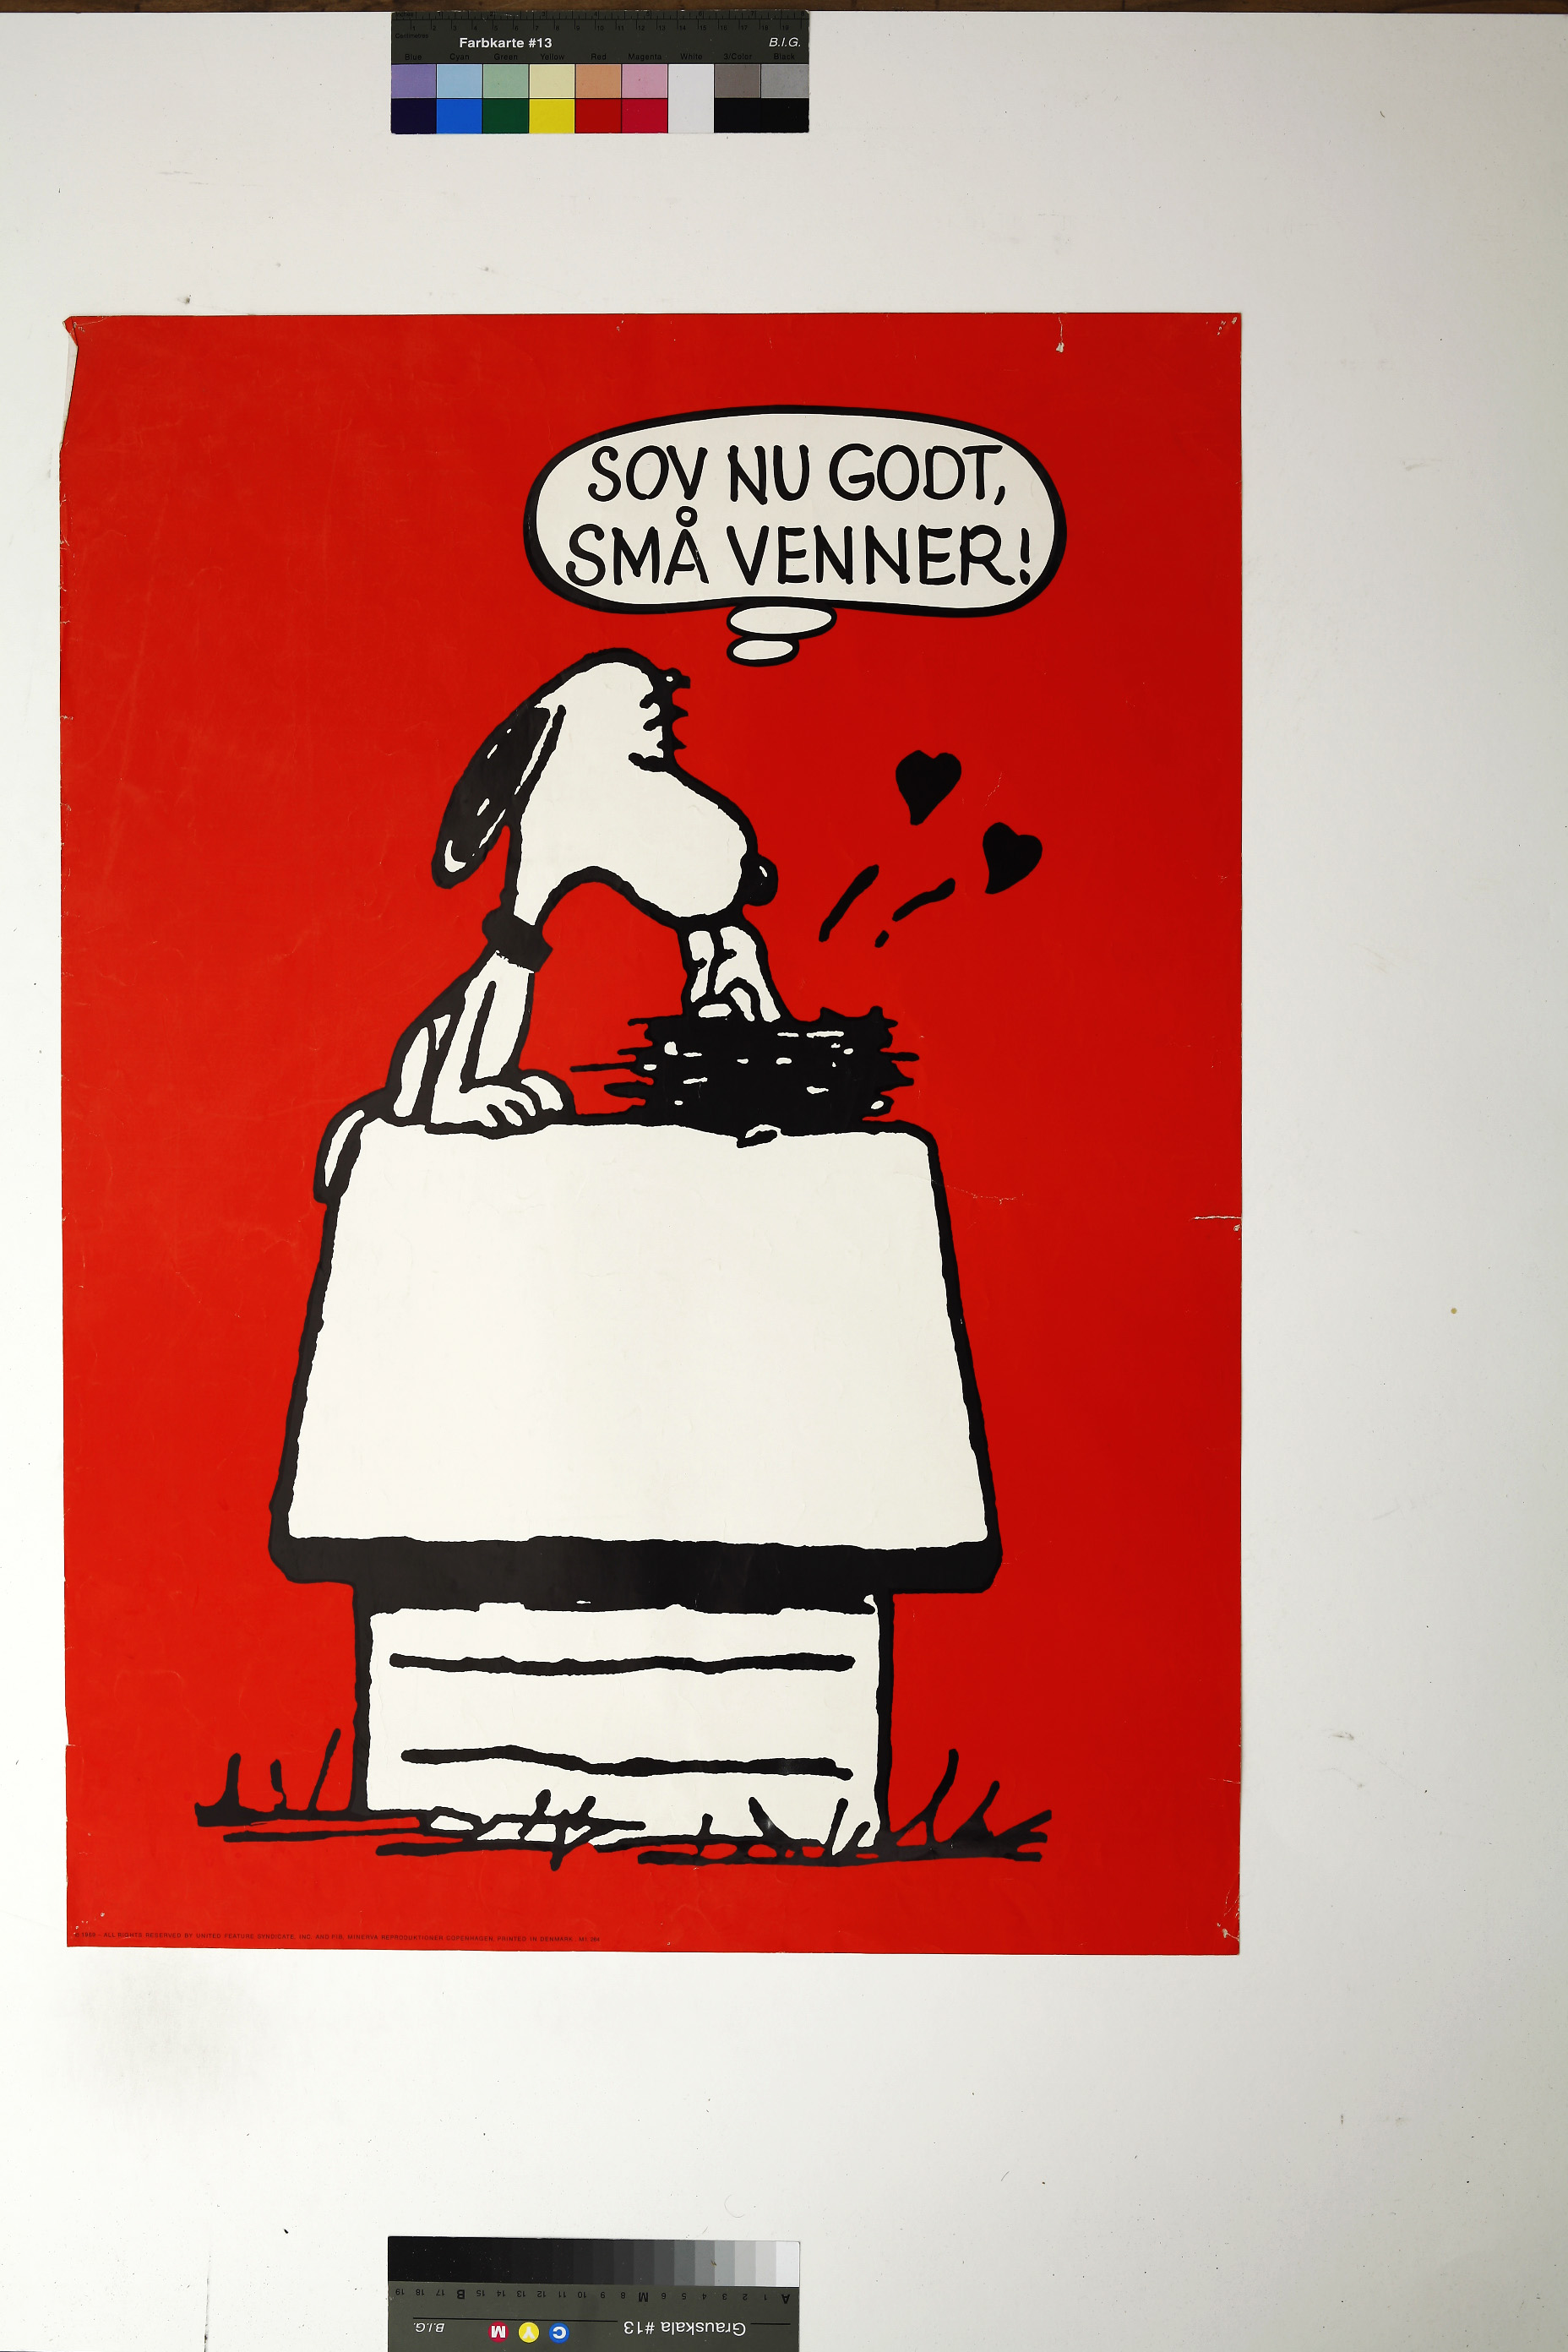
\includegraphics[width=\linewidth]{Abbildung_22_(acht1_063)}
\centering
\caption{Dekoratives Plakat – Peanuts, 1992 (acht1\_063).}
\end{figure}

\newpage
\begin{figure}[ht]
	\begin{subfigure}[b]{\linewidth}
	\centering
	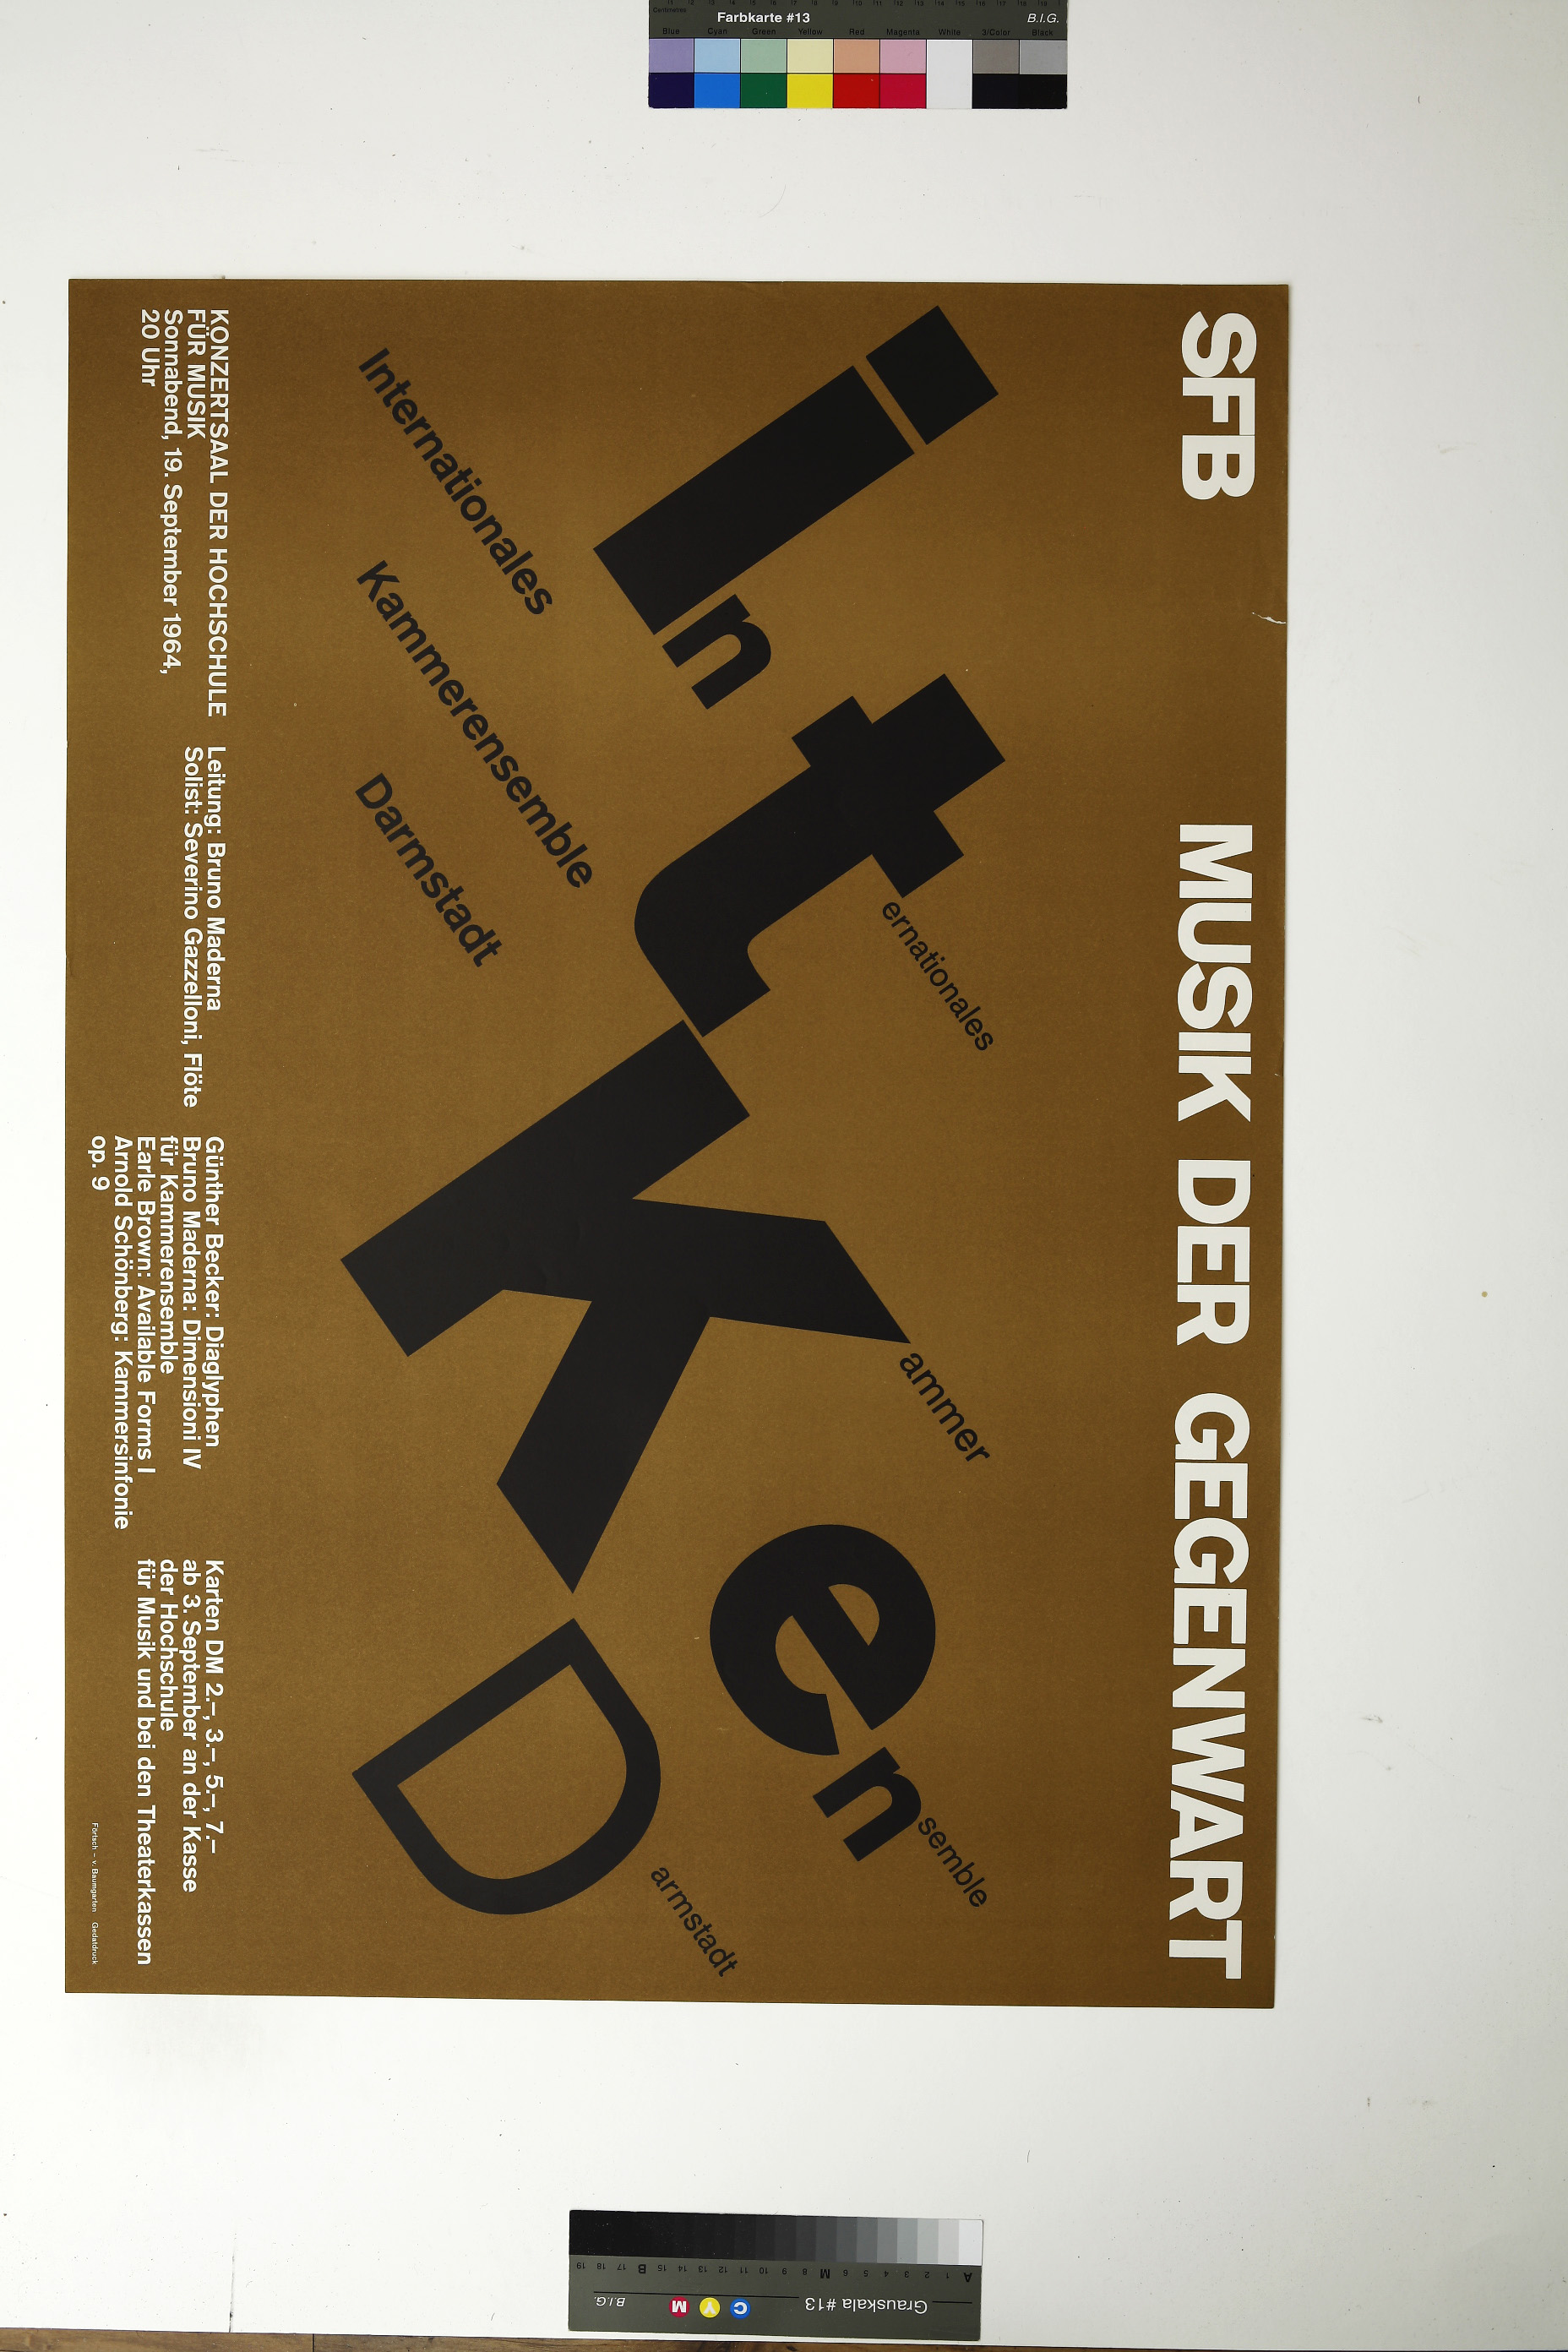
\includegraphics[height=\linewidth, angle=90]{Abbildung_23_(acht2_105)}
	\end{subfigure}
	\begin{subfigure}[b]{\linewidth}
	\centering
	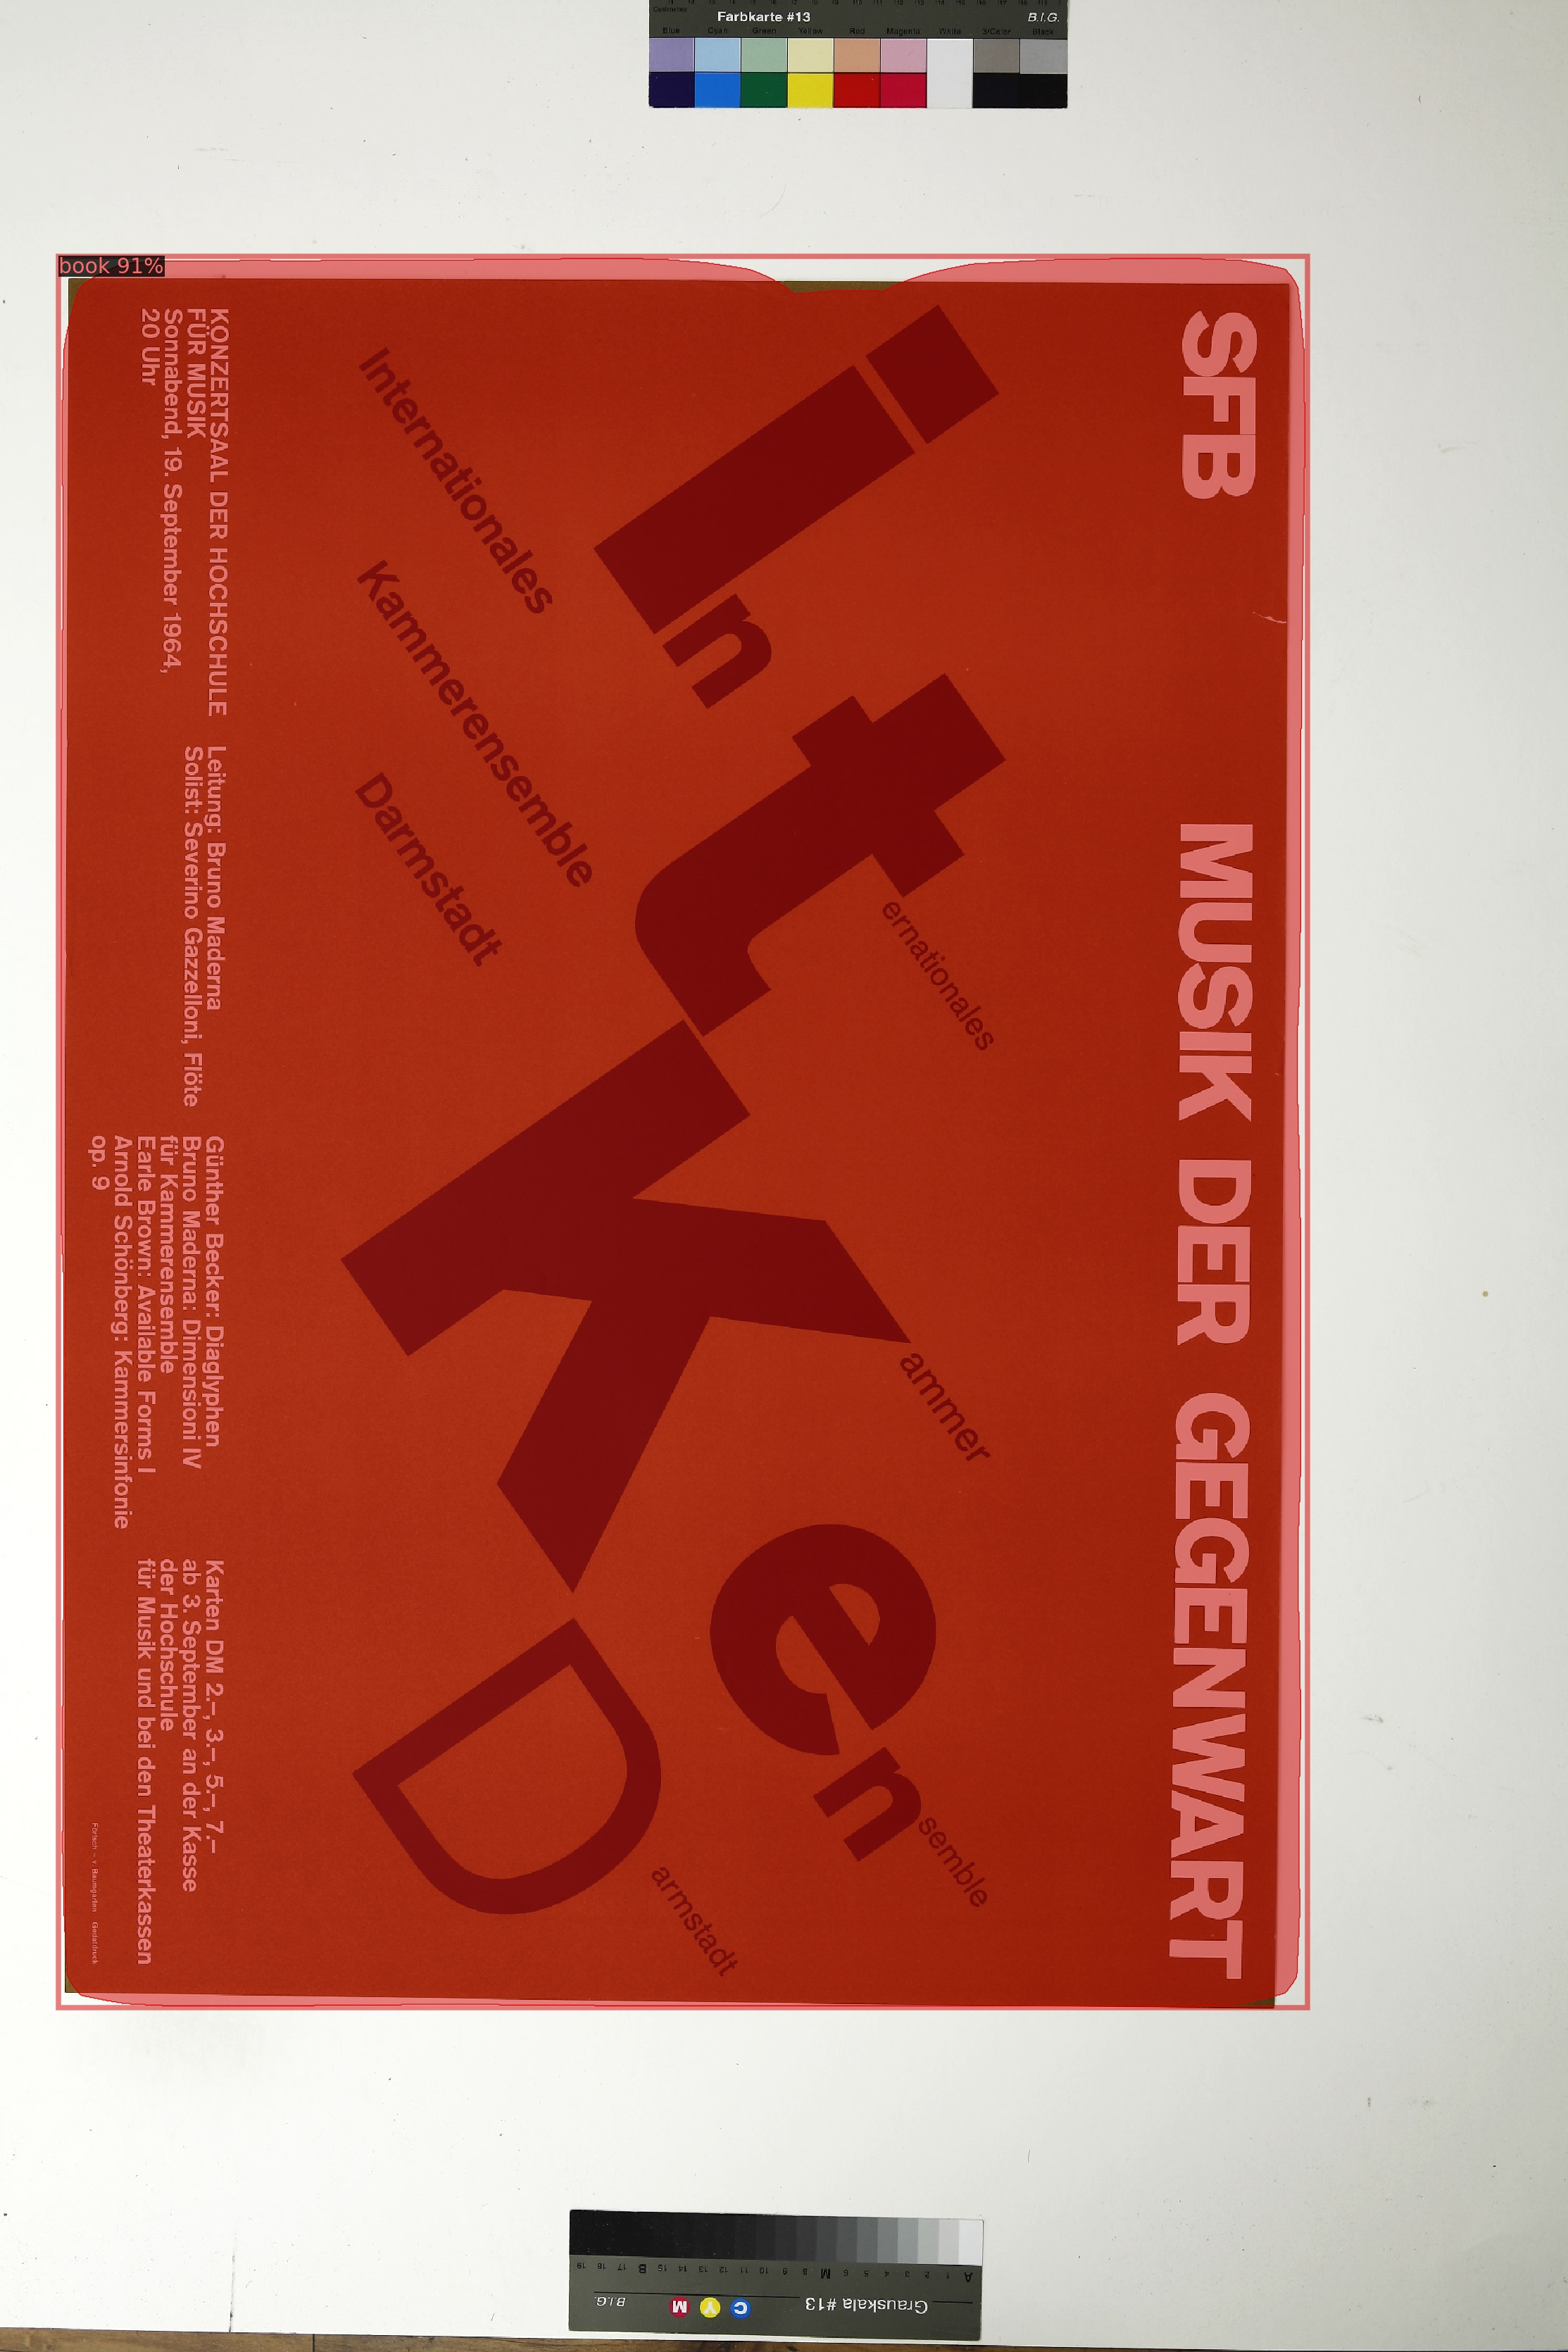
\includegraphics[height=\linewidth, angle=90]{Abbildung_23_(acht2_105)_with_detections}
	\end{subfigure}
	\caption{Veranstaltungsplakat - Musik der Gegenwart, Sender Freies Berlin, 19.09.1964 (acht2\_105); Unten: Mit Annotationen.}
\end{figure}


\newpage
\begin{landscape}
\begin{figure}[ht]
	\begin{subfigure}[b]{0.5\linewidth}
	\centering
	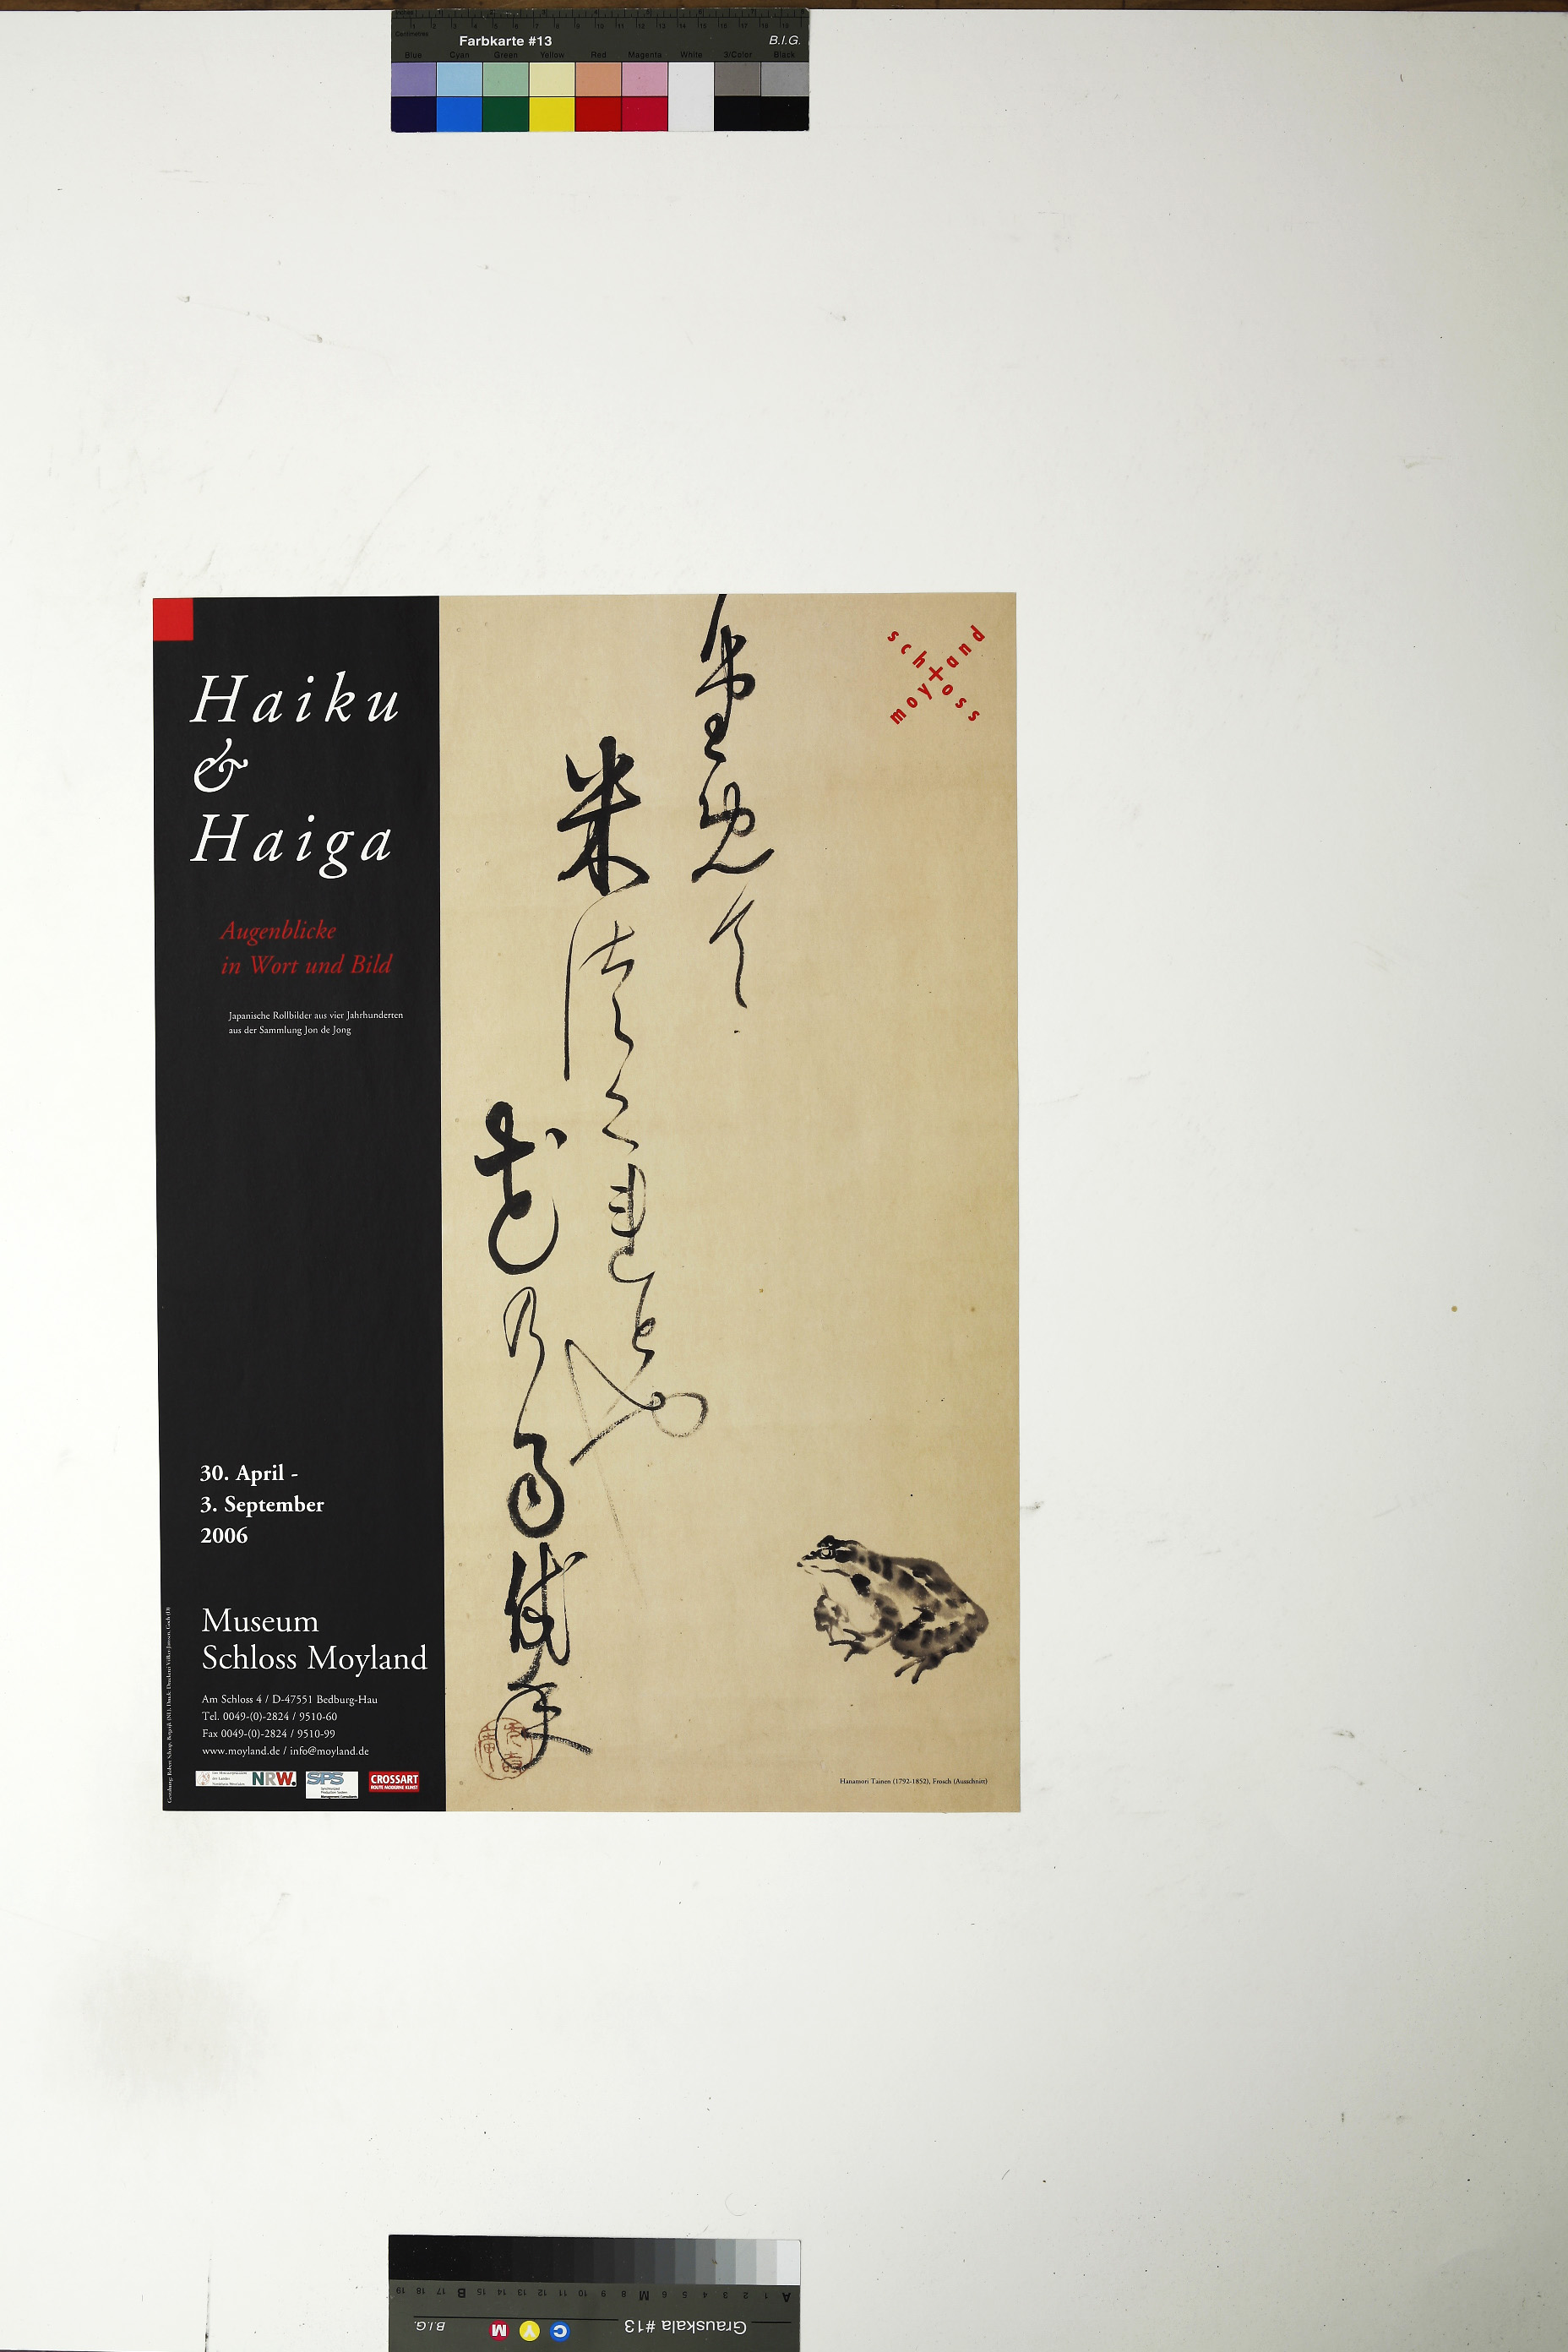
\includegraphics[height=\linewidth]{Abbildung_24_(acht1_109)}
	\end{subfigure}
	\begin{subfigure}[b]{0.5\linewidth}
	\centering
	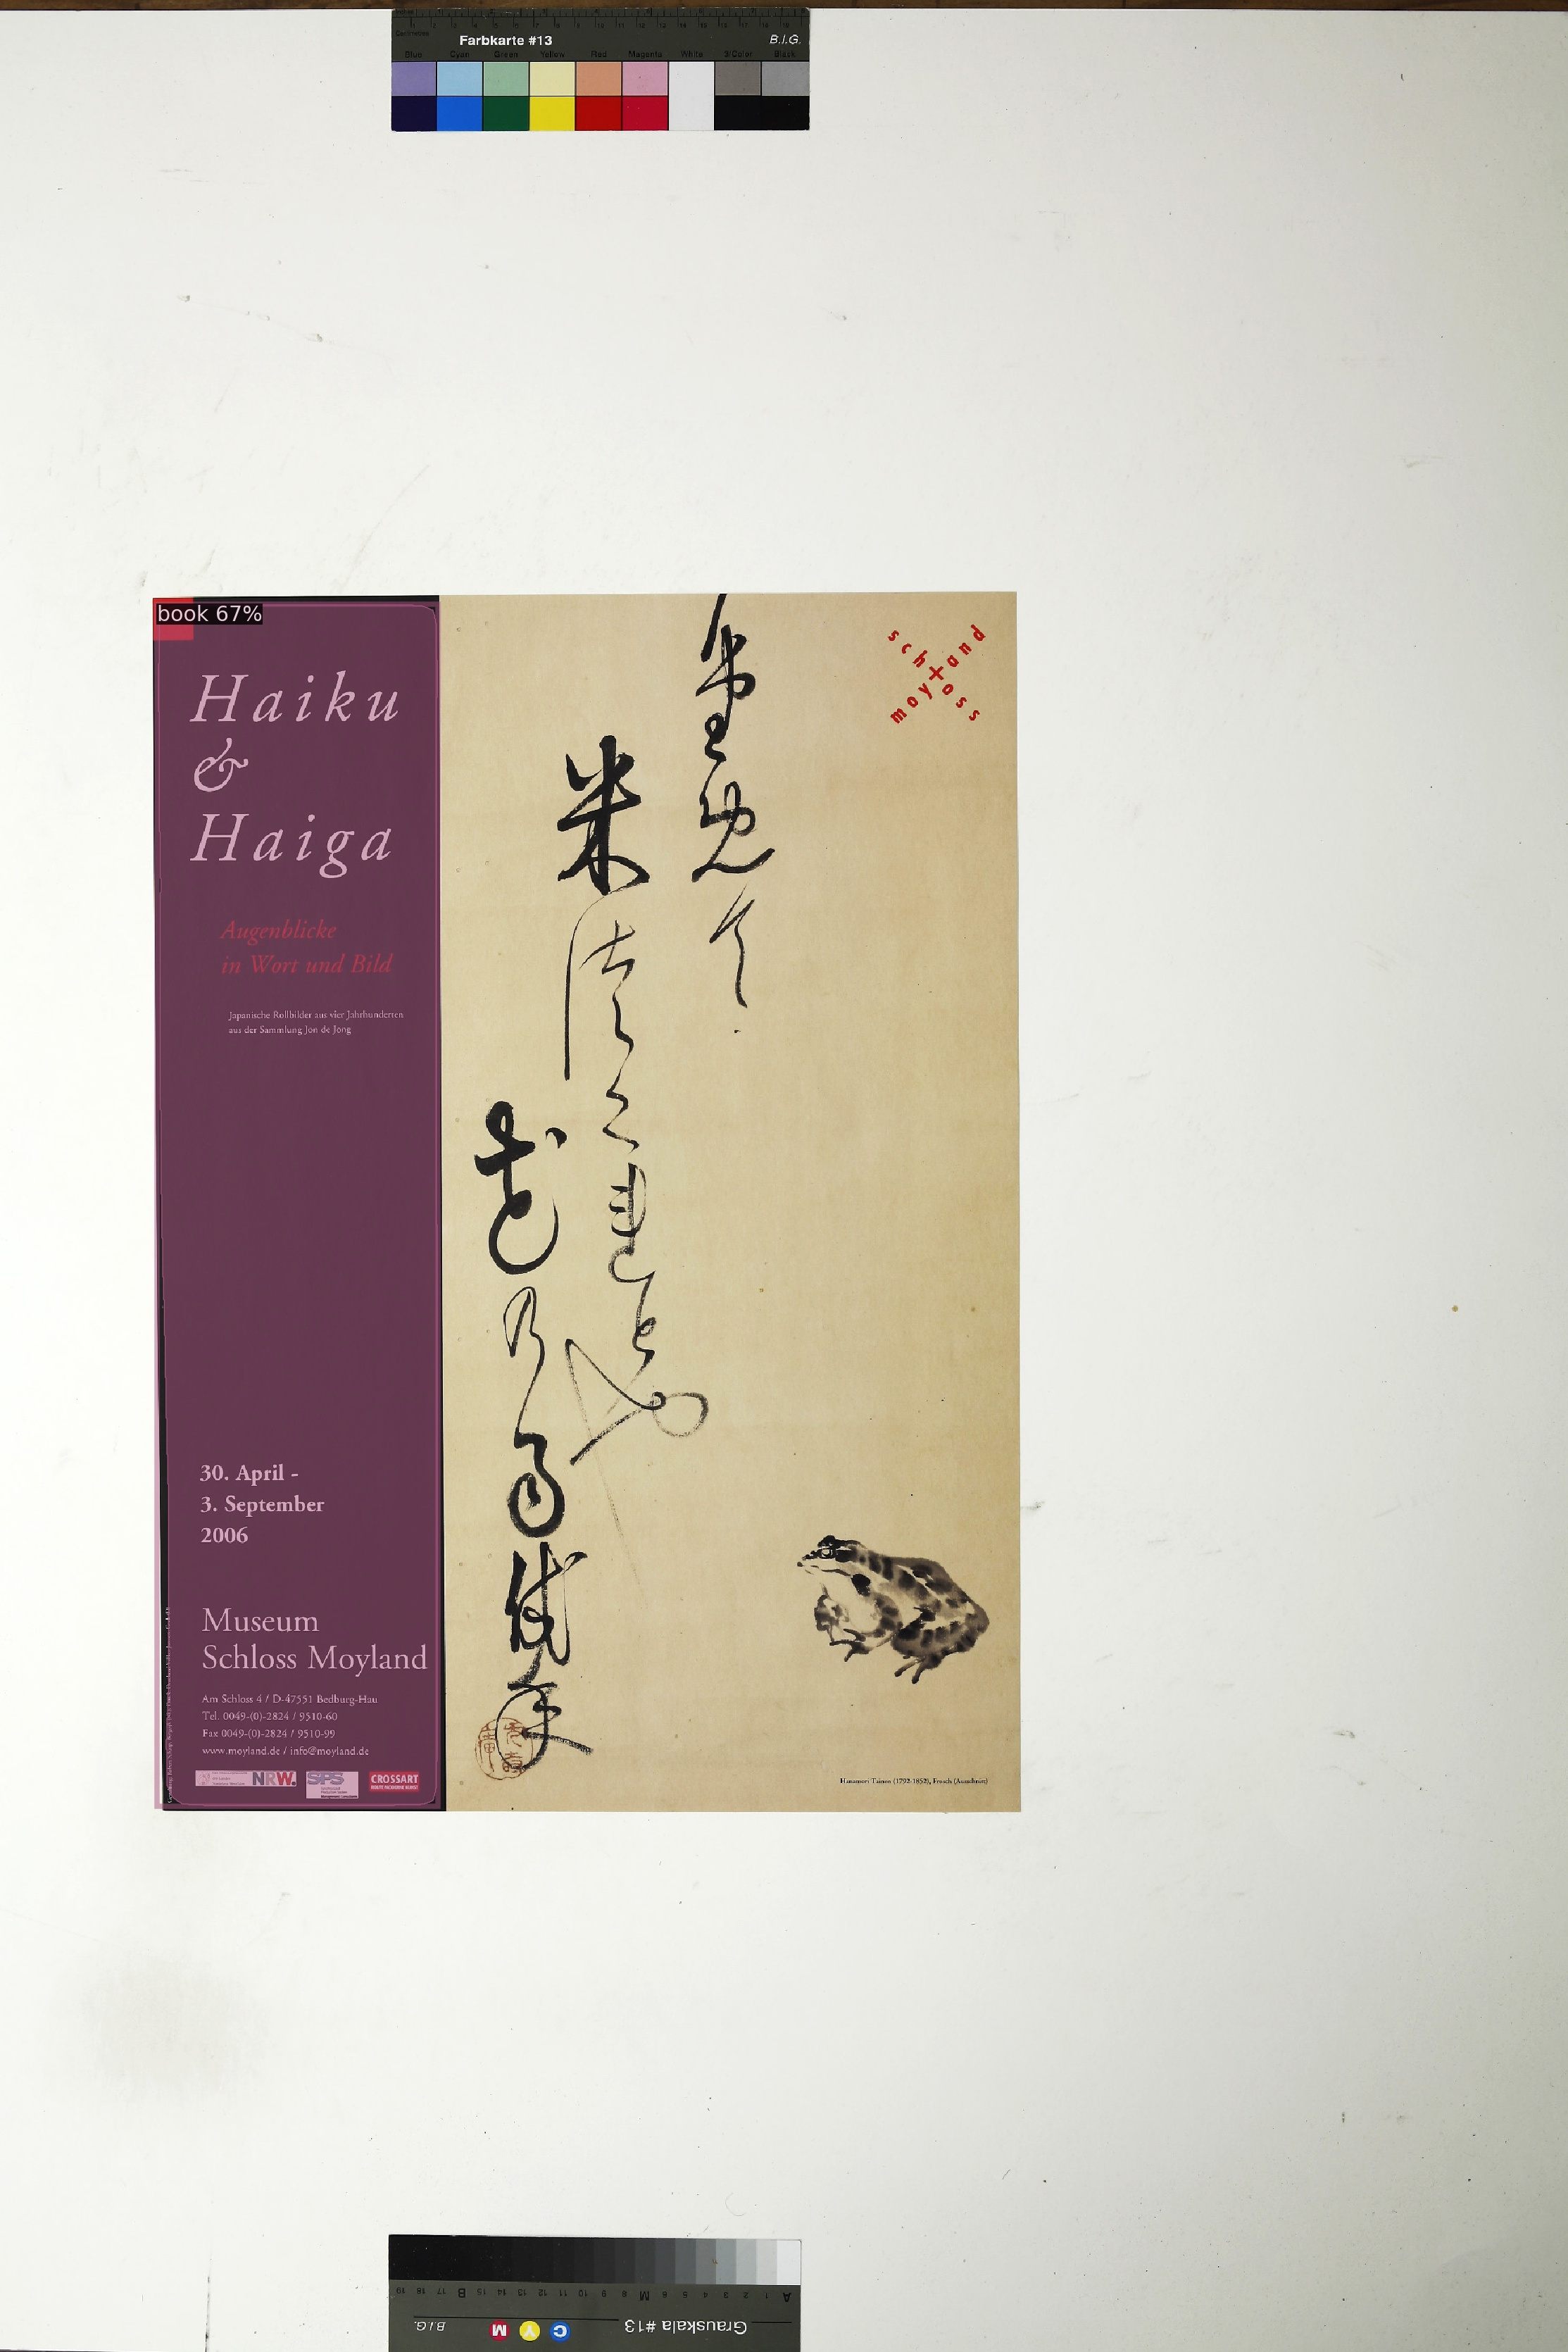
\includegraphics[height=\linewidth]{Abbildung_24_(acht1_109)_with_detections}
	\end{subfigure}
	\caption{Ausstellungsplakat – Haiku \& Haiga, Museum Schloss Moyland, 30.04.2006-03.09.2006 (acht1\_109); Rechts: Mit Annotationen.}
\end{figure}
\end{landscape}

\newpage
\begin{landscape}
\begin{figure}[ht]
	\begin{subfigure}[b]{0.5\linewidth}
	\centering
	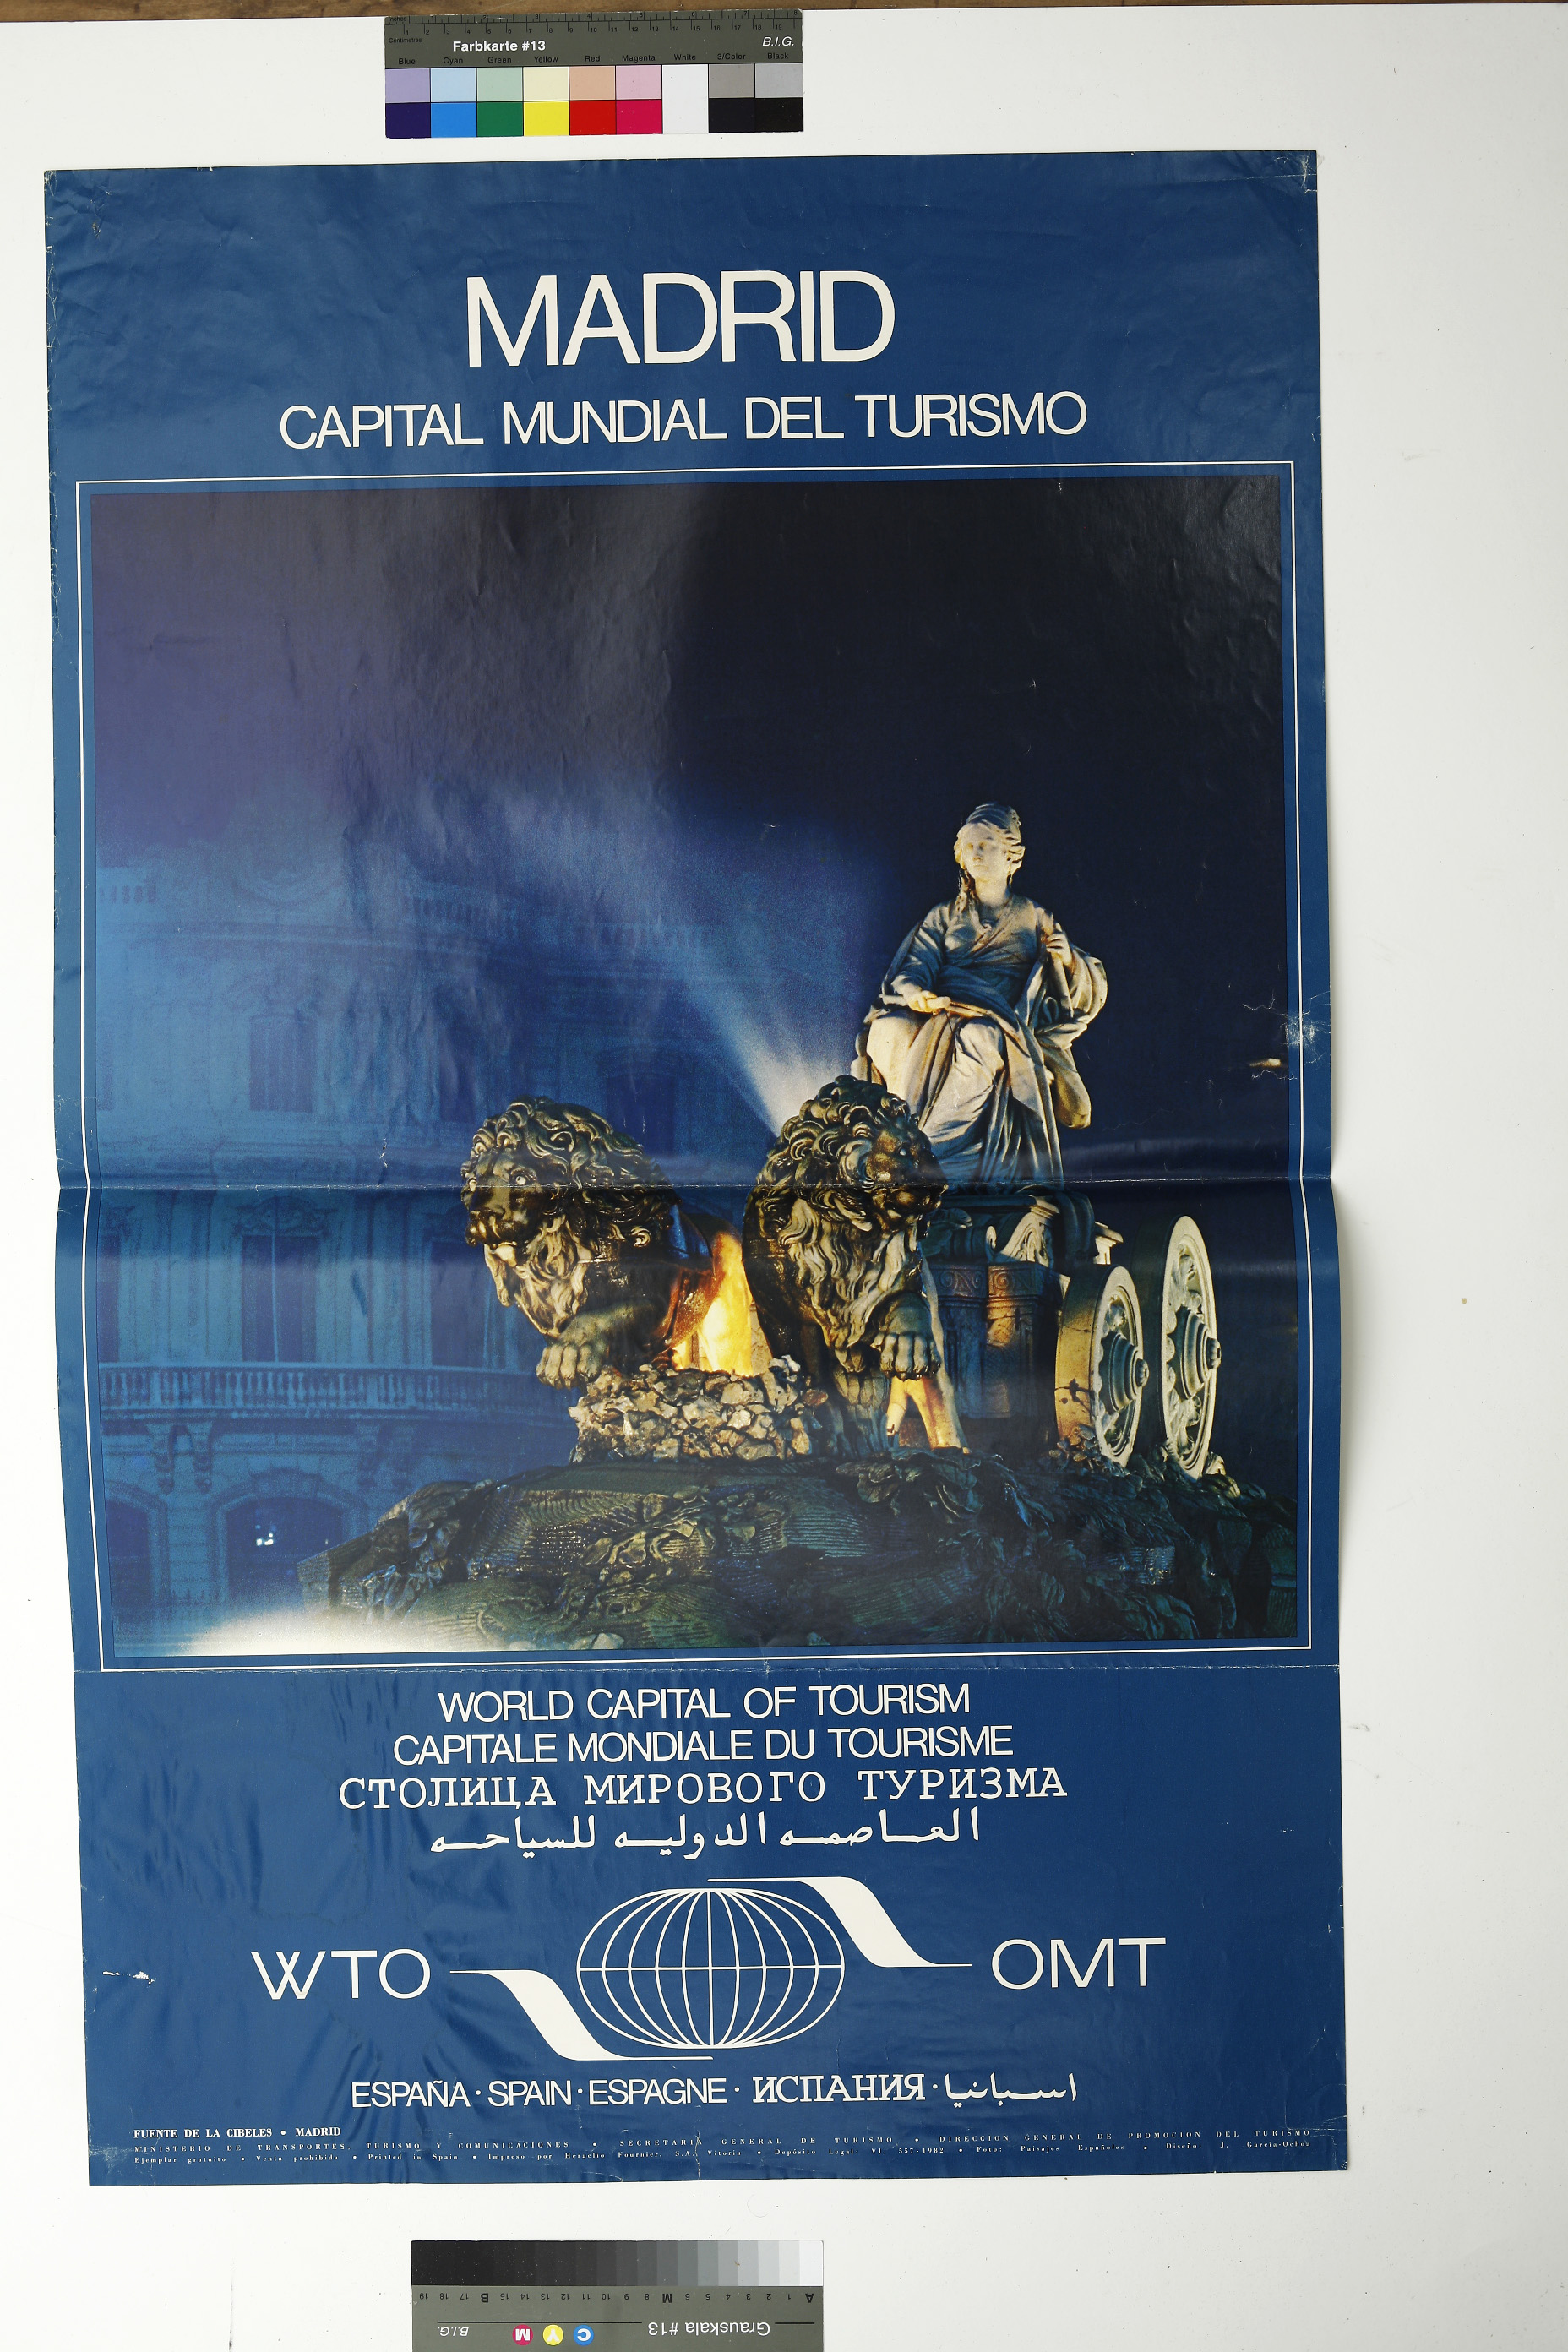
\includegraphics[height=\linewidth]{Abbildung_25_(acht1_165)}
	\end{subfigure}
	\begin{subfigure}[b]{0.5\linewidth}
	\centering
	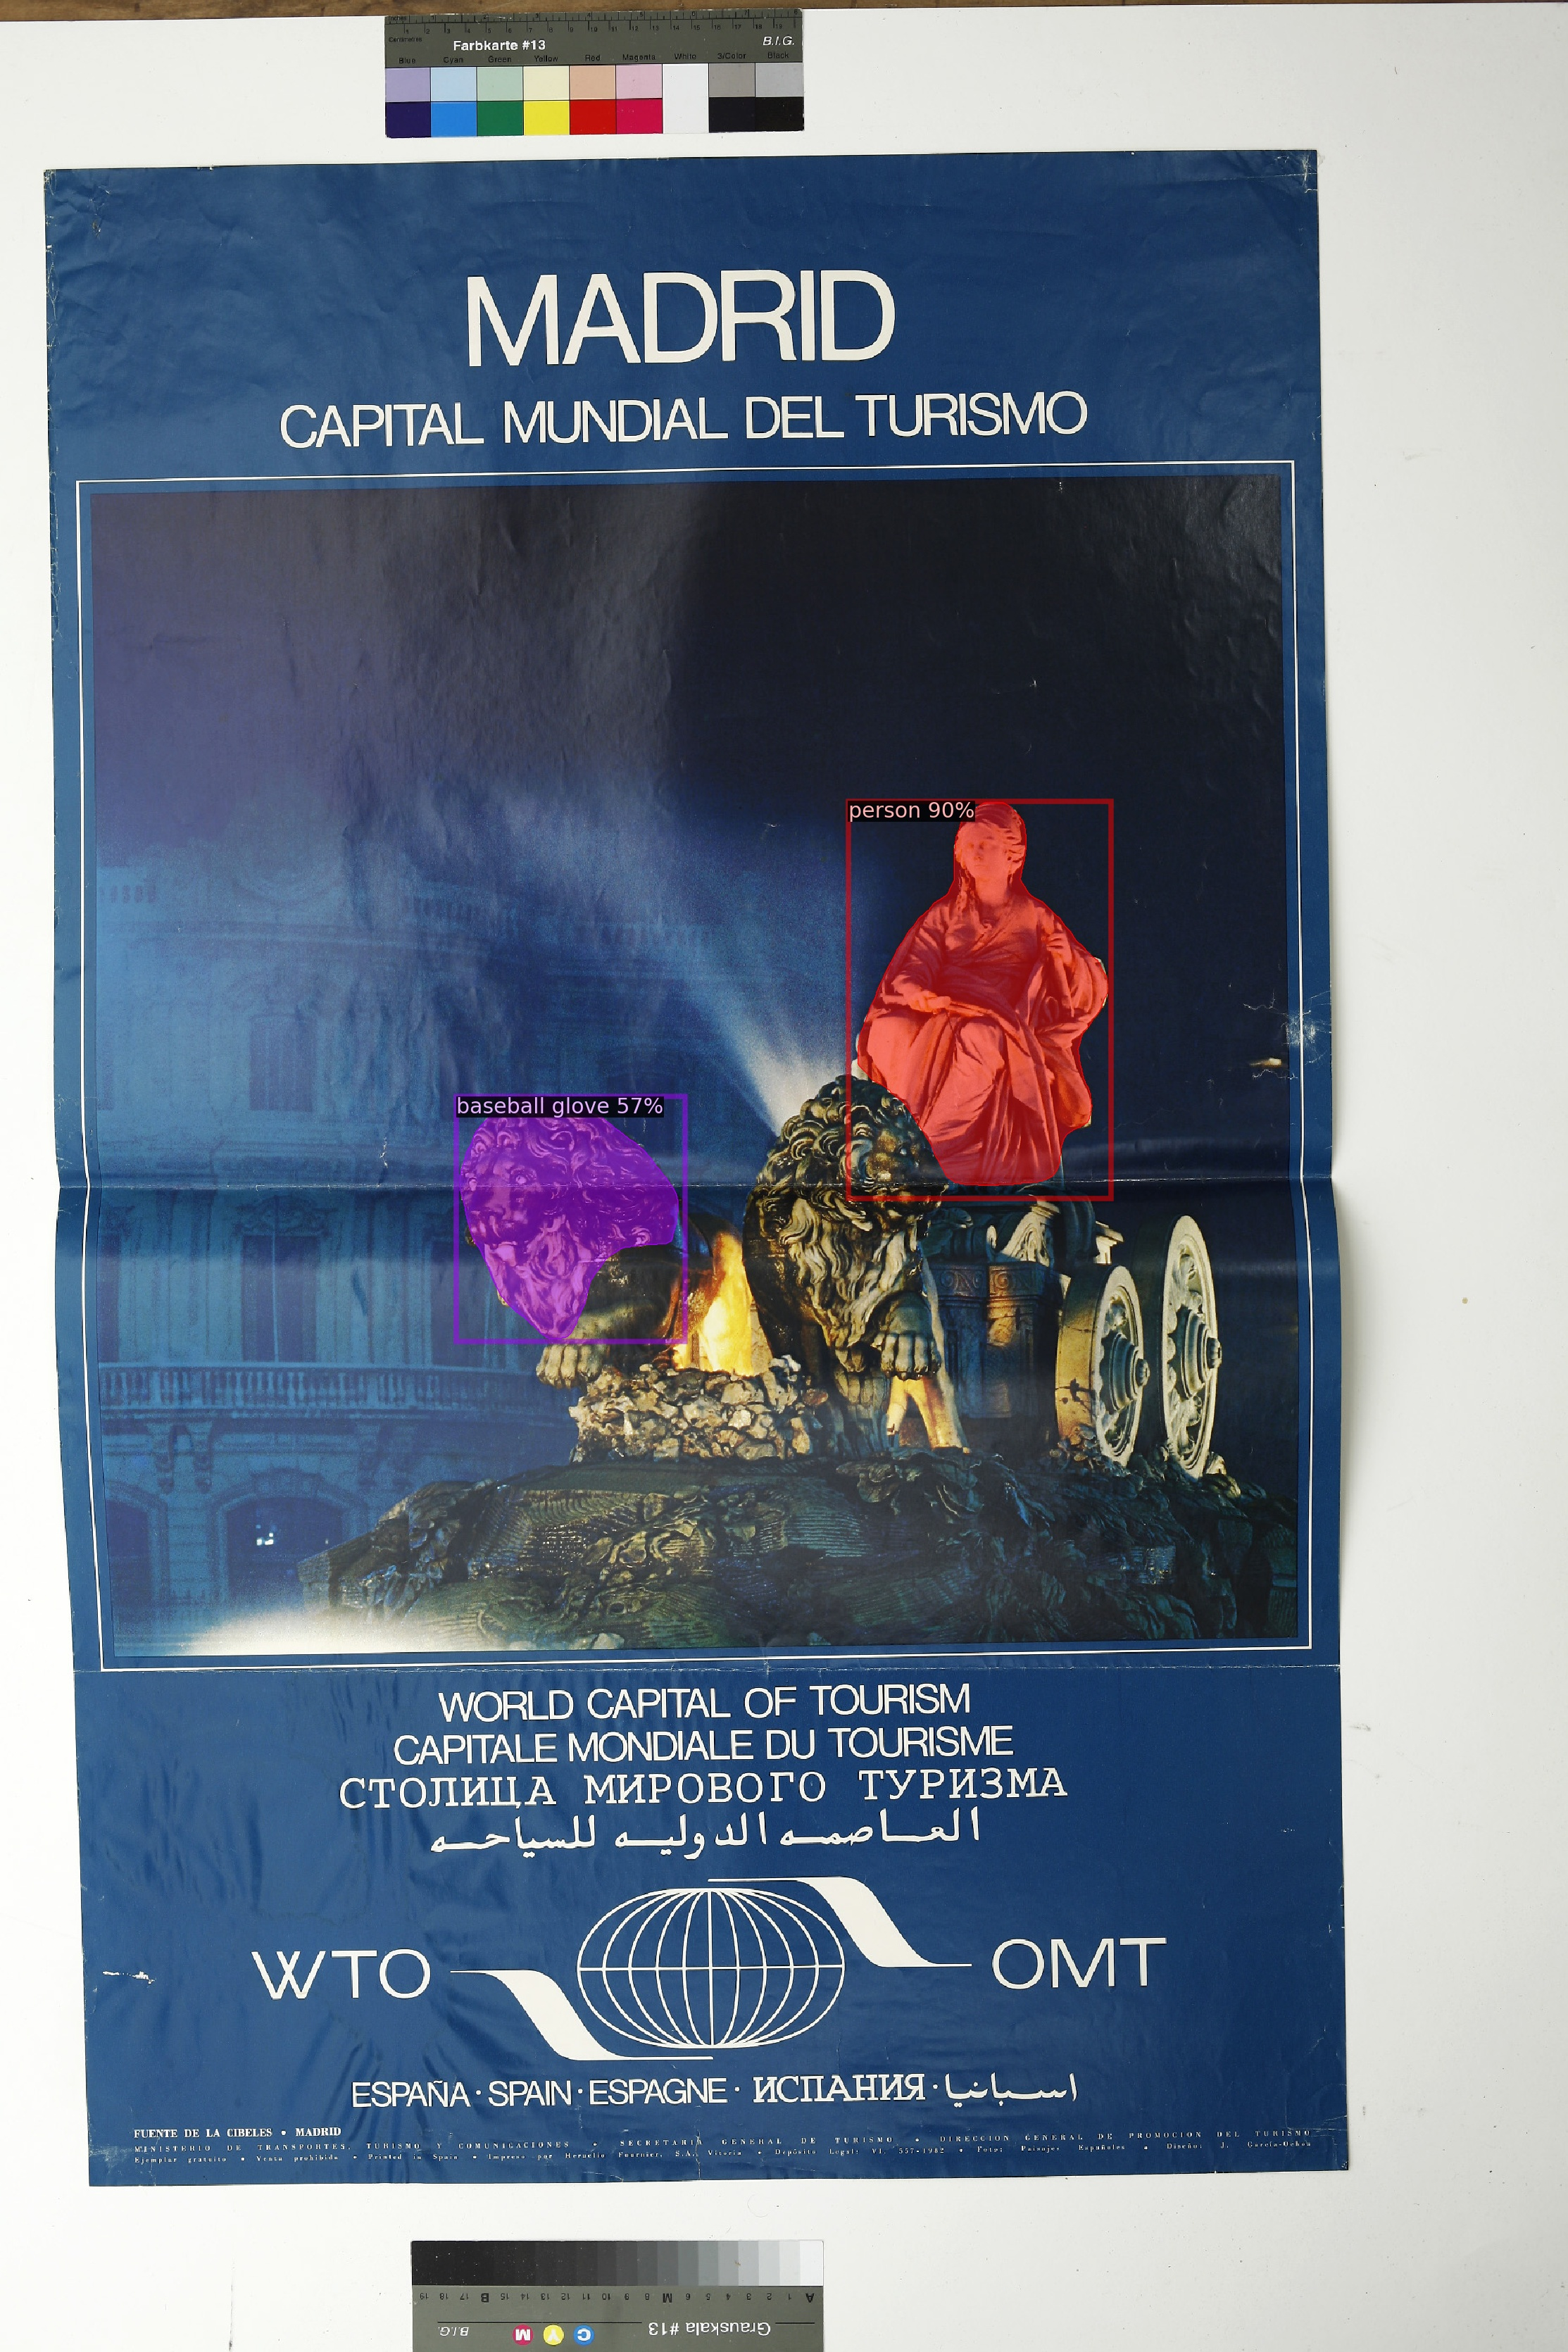
\includegraphics[height=\linewidth]{Abbildung_25_(acht1_165)_with_detections}
	\end{subfigure}
	\caption{Werbeplakat –Madrid. Capital Mundial del Turismo, Ministerio de Transportes, Turismo y Comunicaciones, ohne Datum (acht1\_165); Rechts: Mit Annotationen.}
\end{figure}
\end{landscape}

\newpage
\begin{landscape}
\begin{figure}[ht]
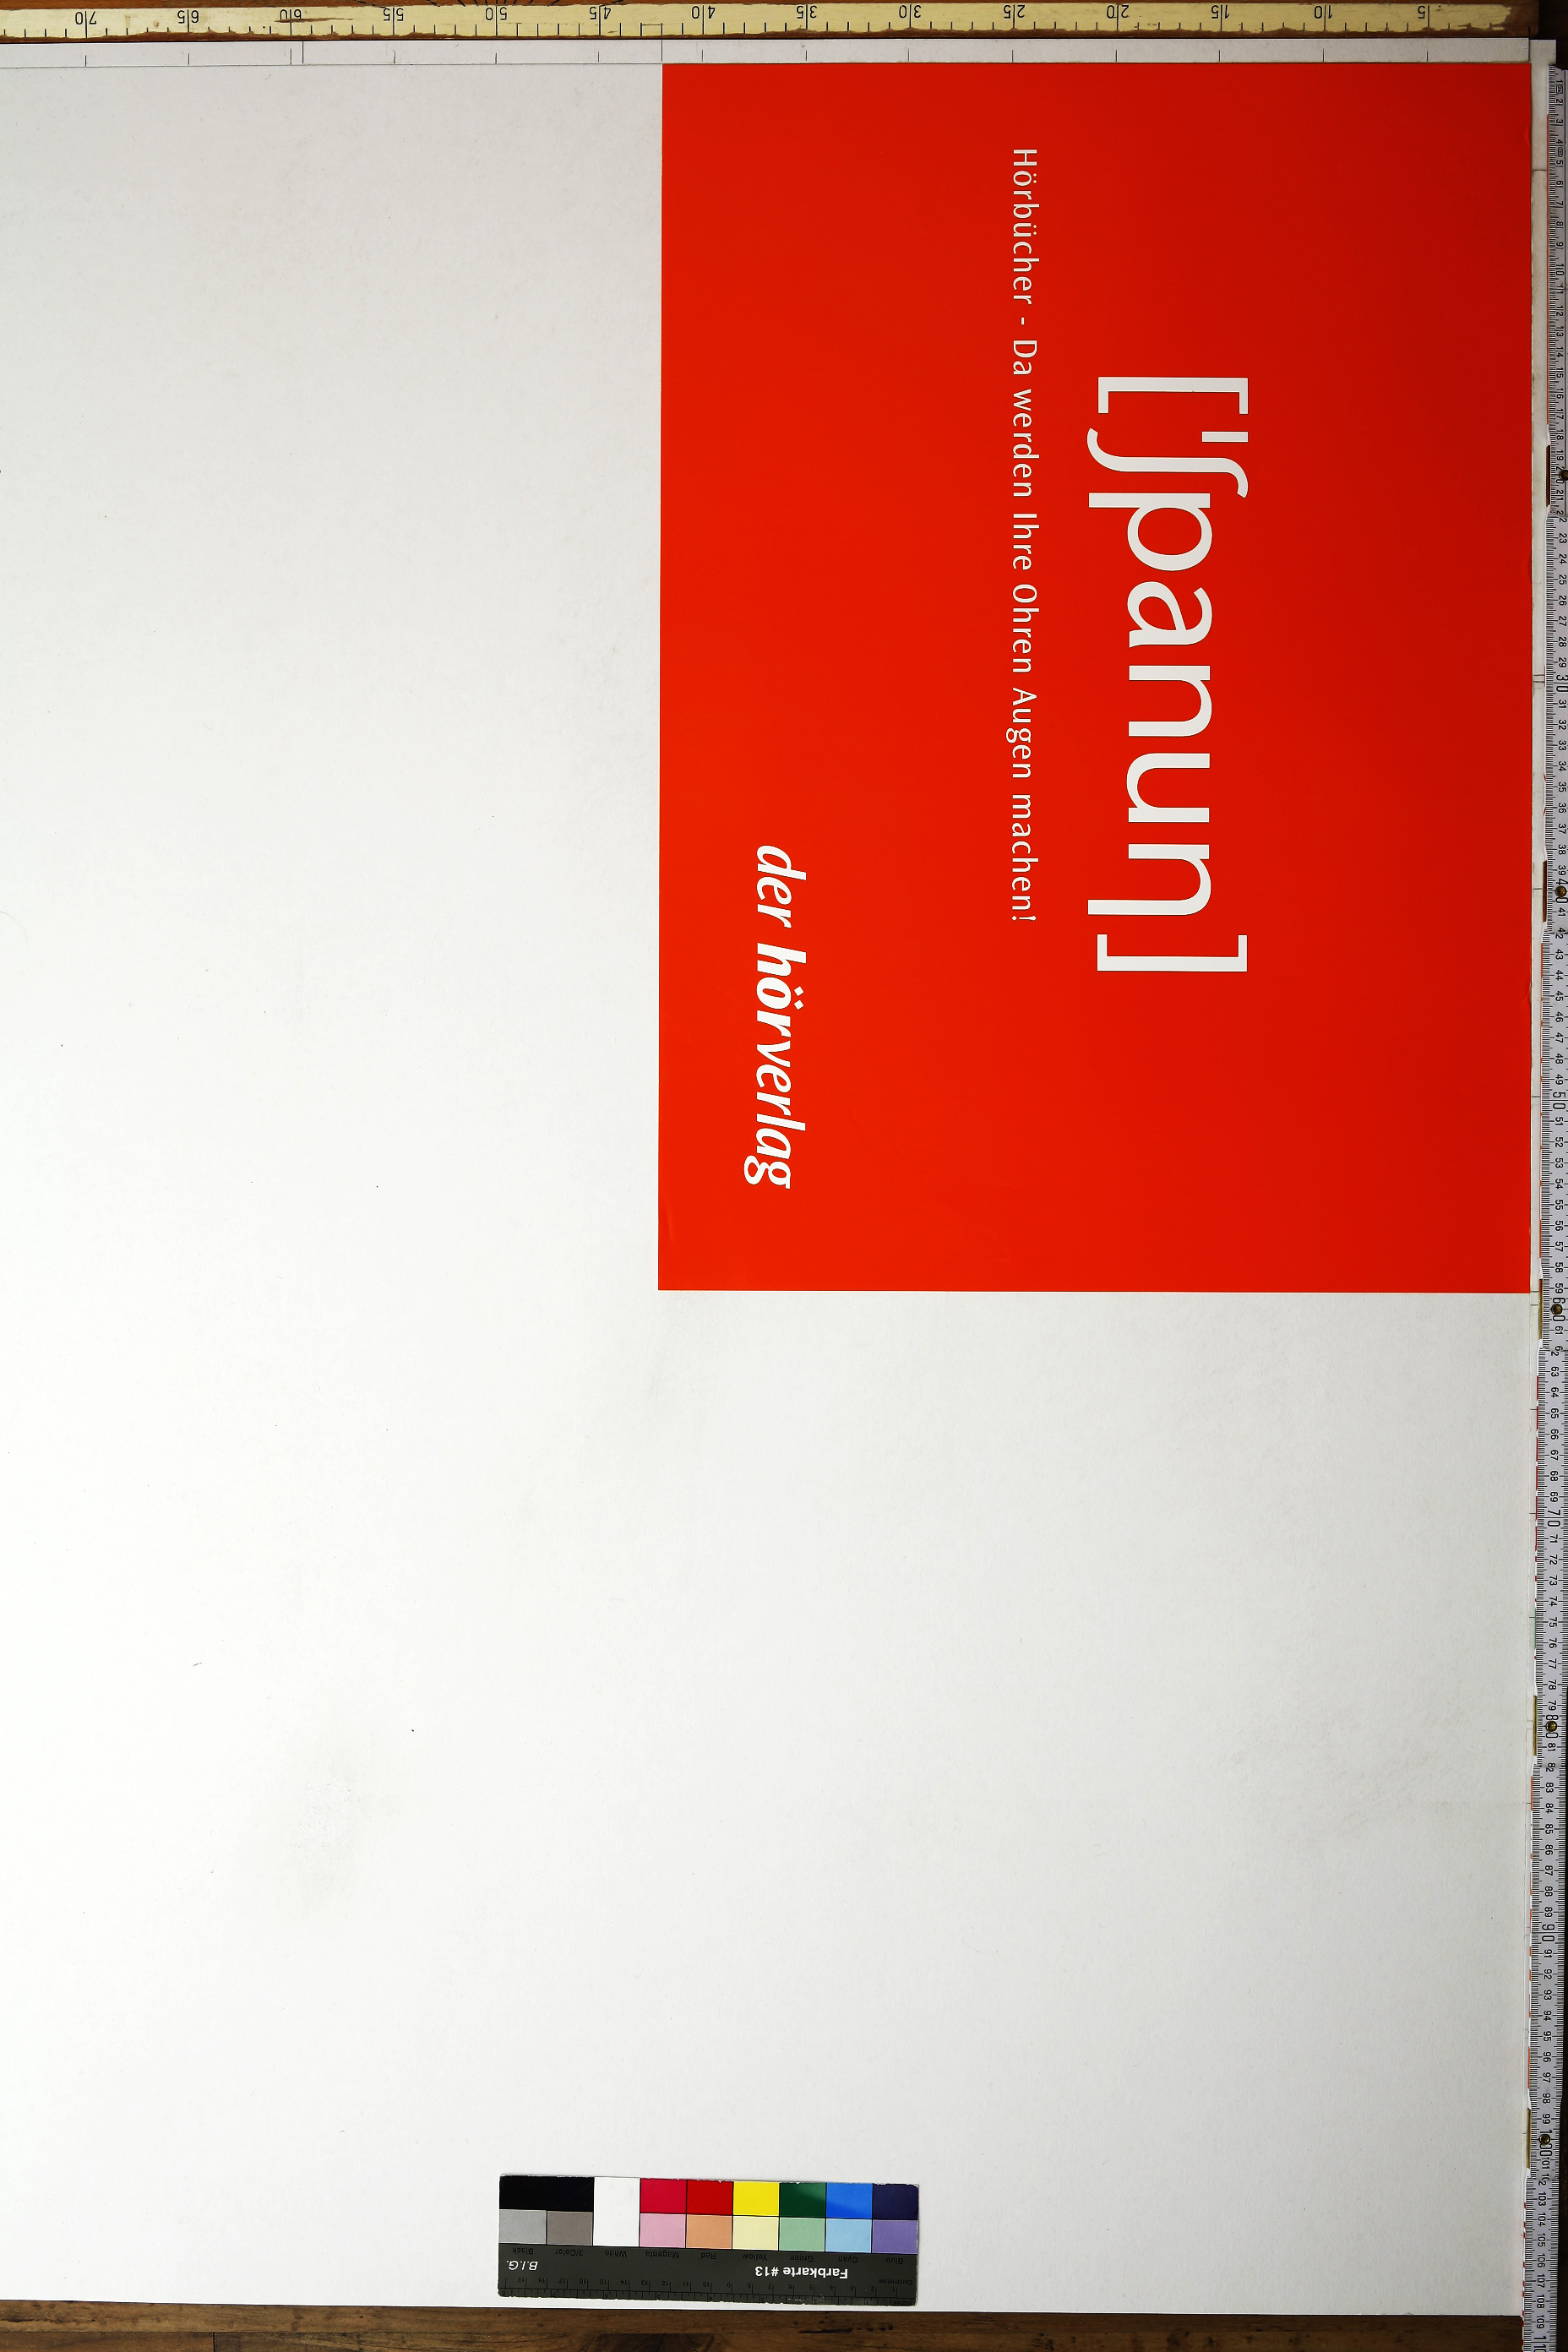
\includegraphics[height=0.85\linewidth, angle=90]{Abbildung_26_(acht3_313)}
\centering
\caption{Werbeplakat – Hörbücher. Da werden Ihre Ohren Augen machen!, der hörverlag, ohne Datum (acht3\_313).}
\end{figure}
\end{landscape}

\newpage
\begin{landscape}
\begin{figure}[ht]
	\begin{subfigure}[b]{0.5\linewidth}
	\centering
	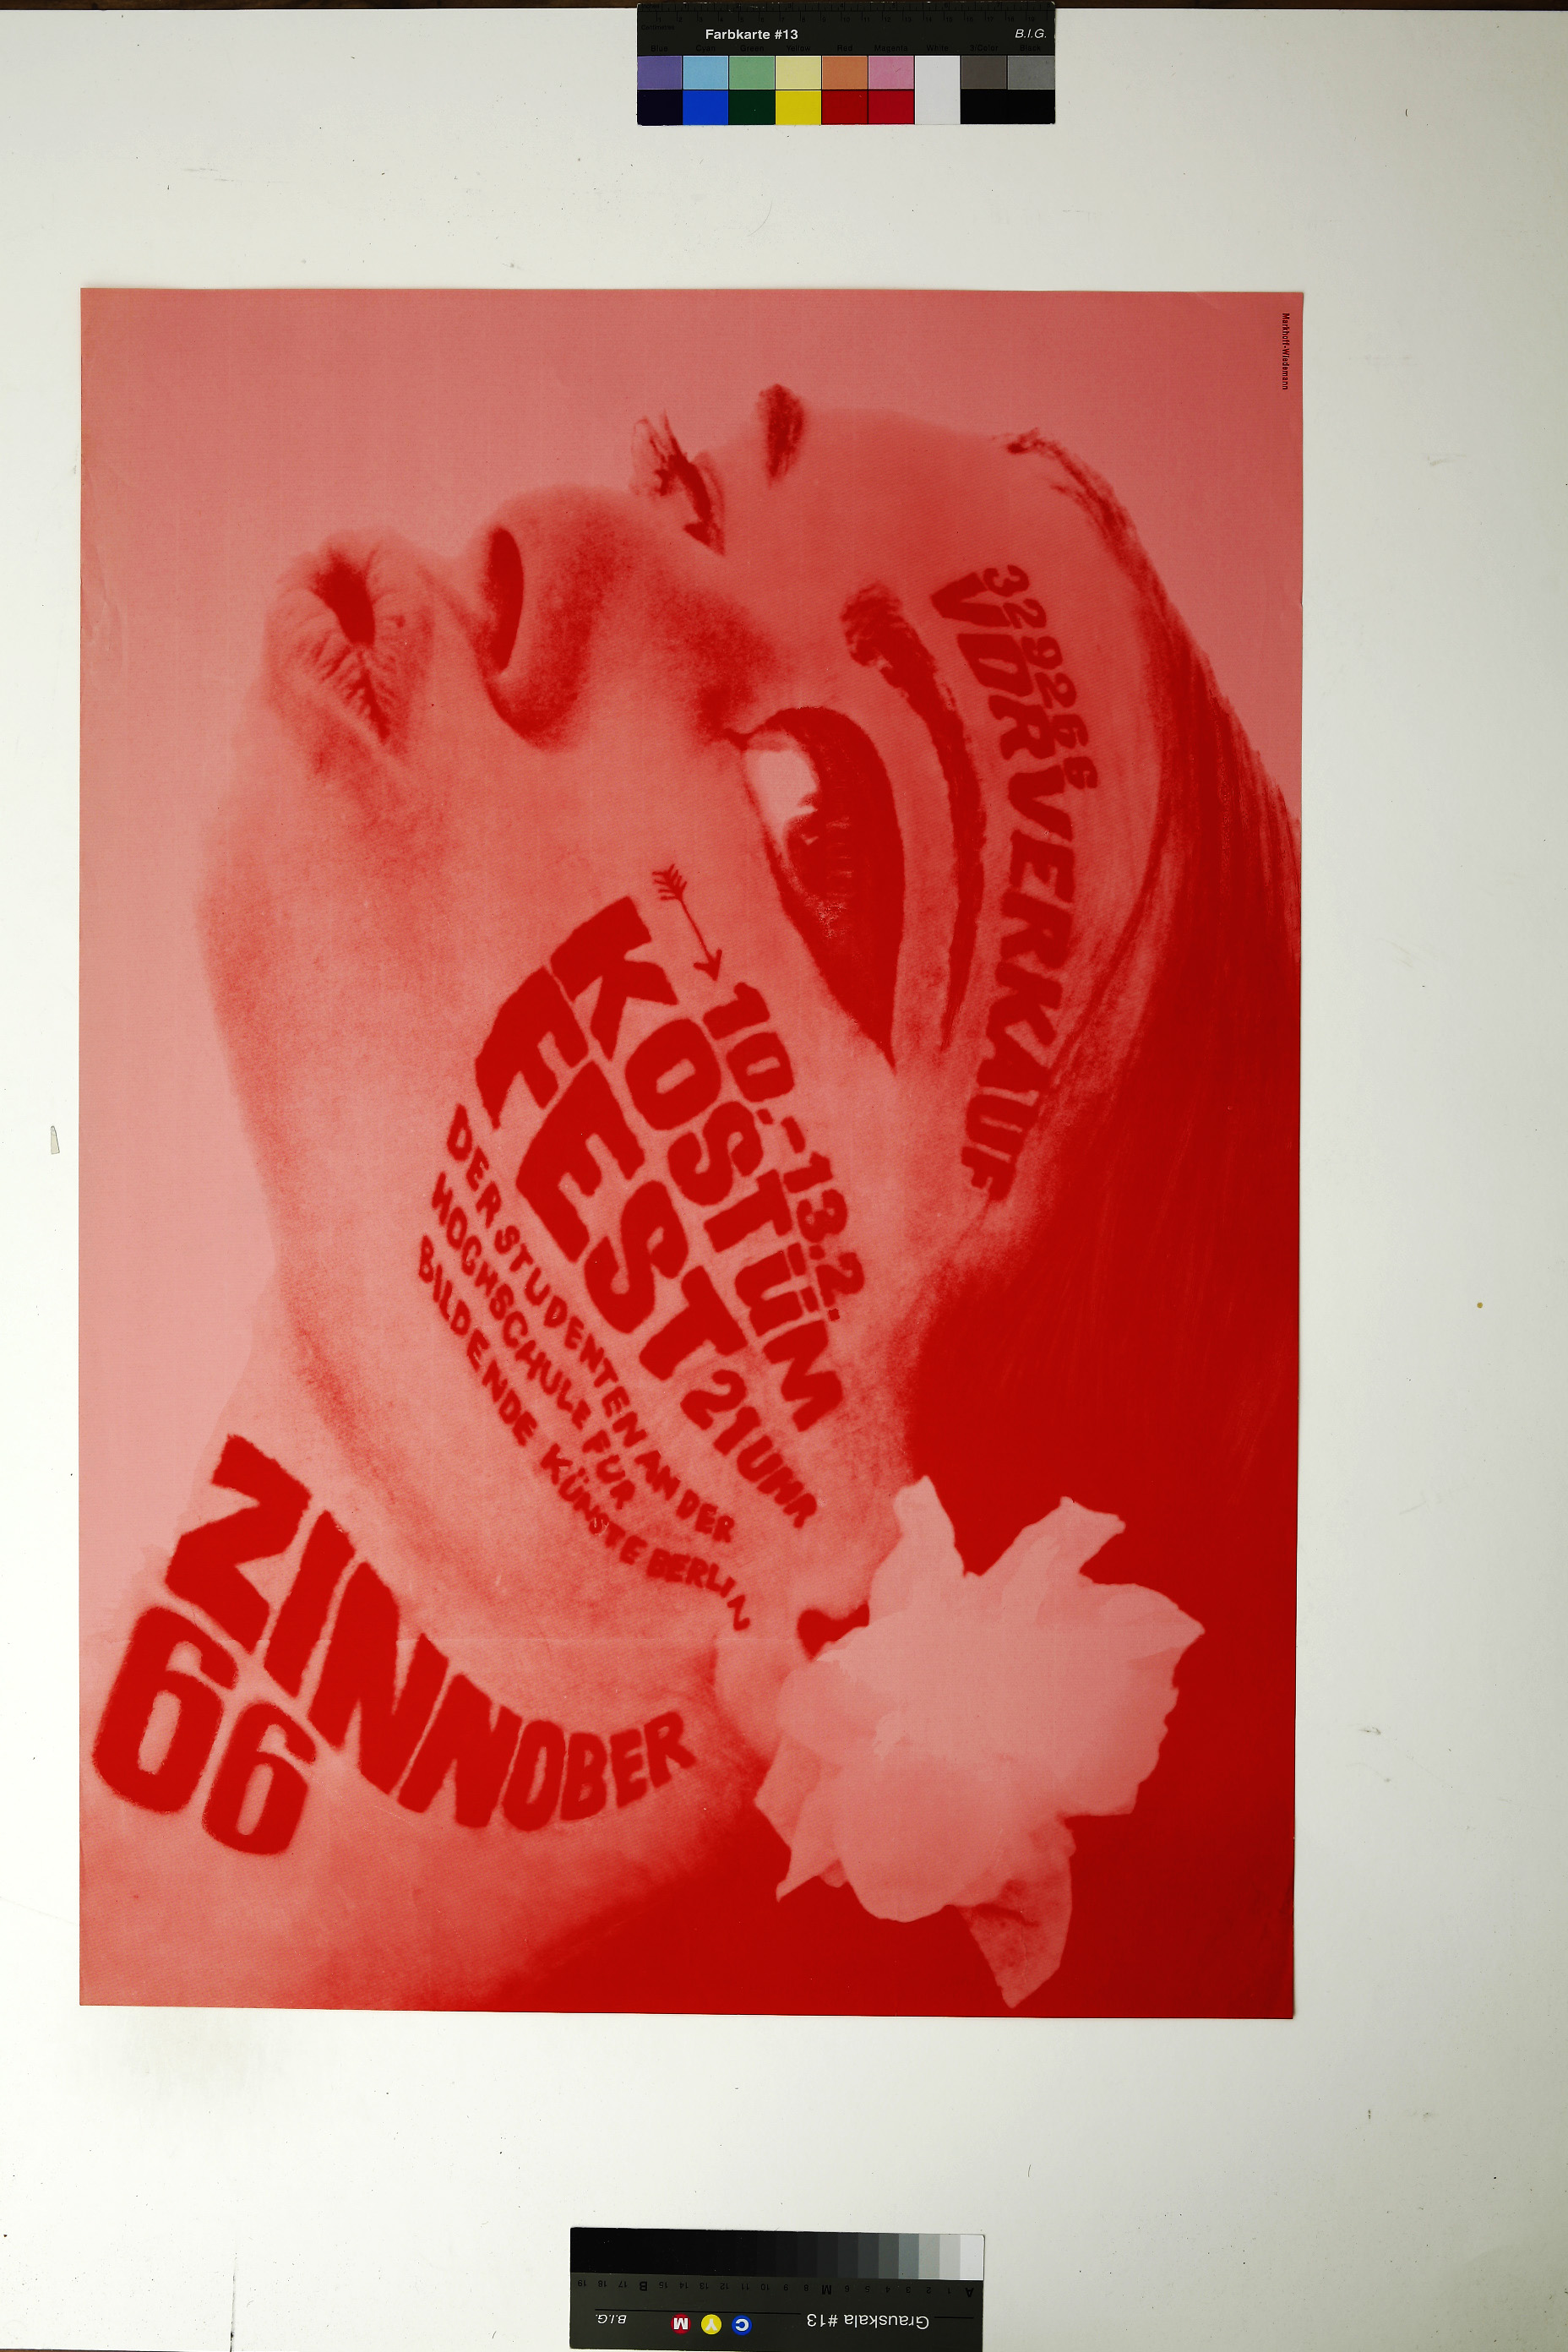
\includegraphics[height=\linewidth]{Abbildung_27_(acht2_068)}
	\end{subfigure}
	\begin{subfigure}[b]{0.5\linewidth}
	\centering
	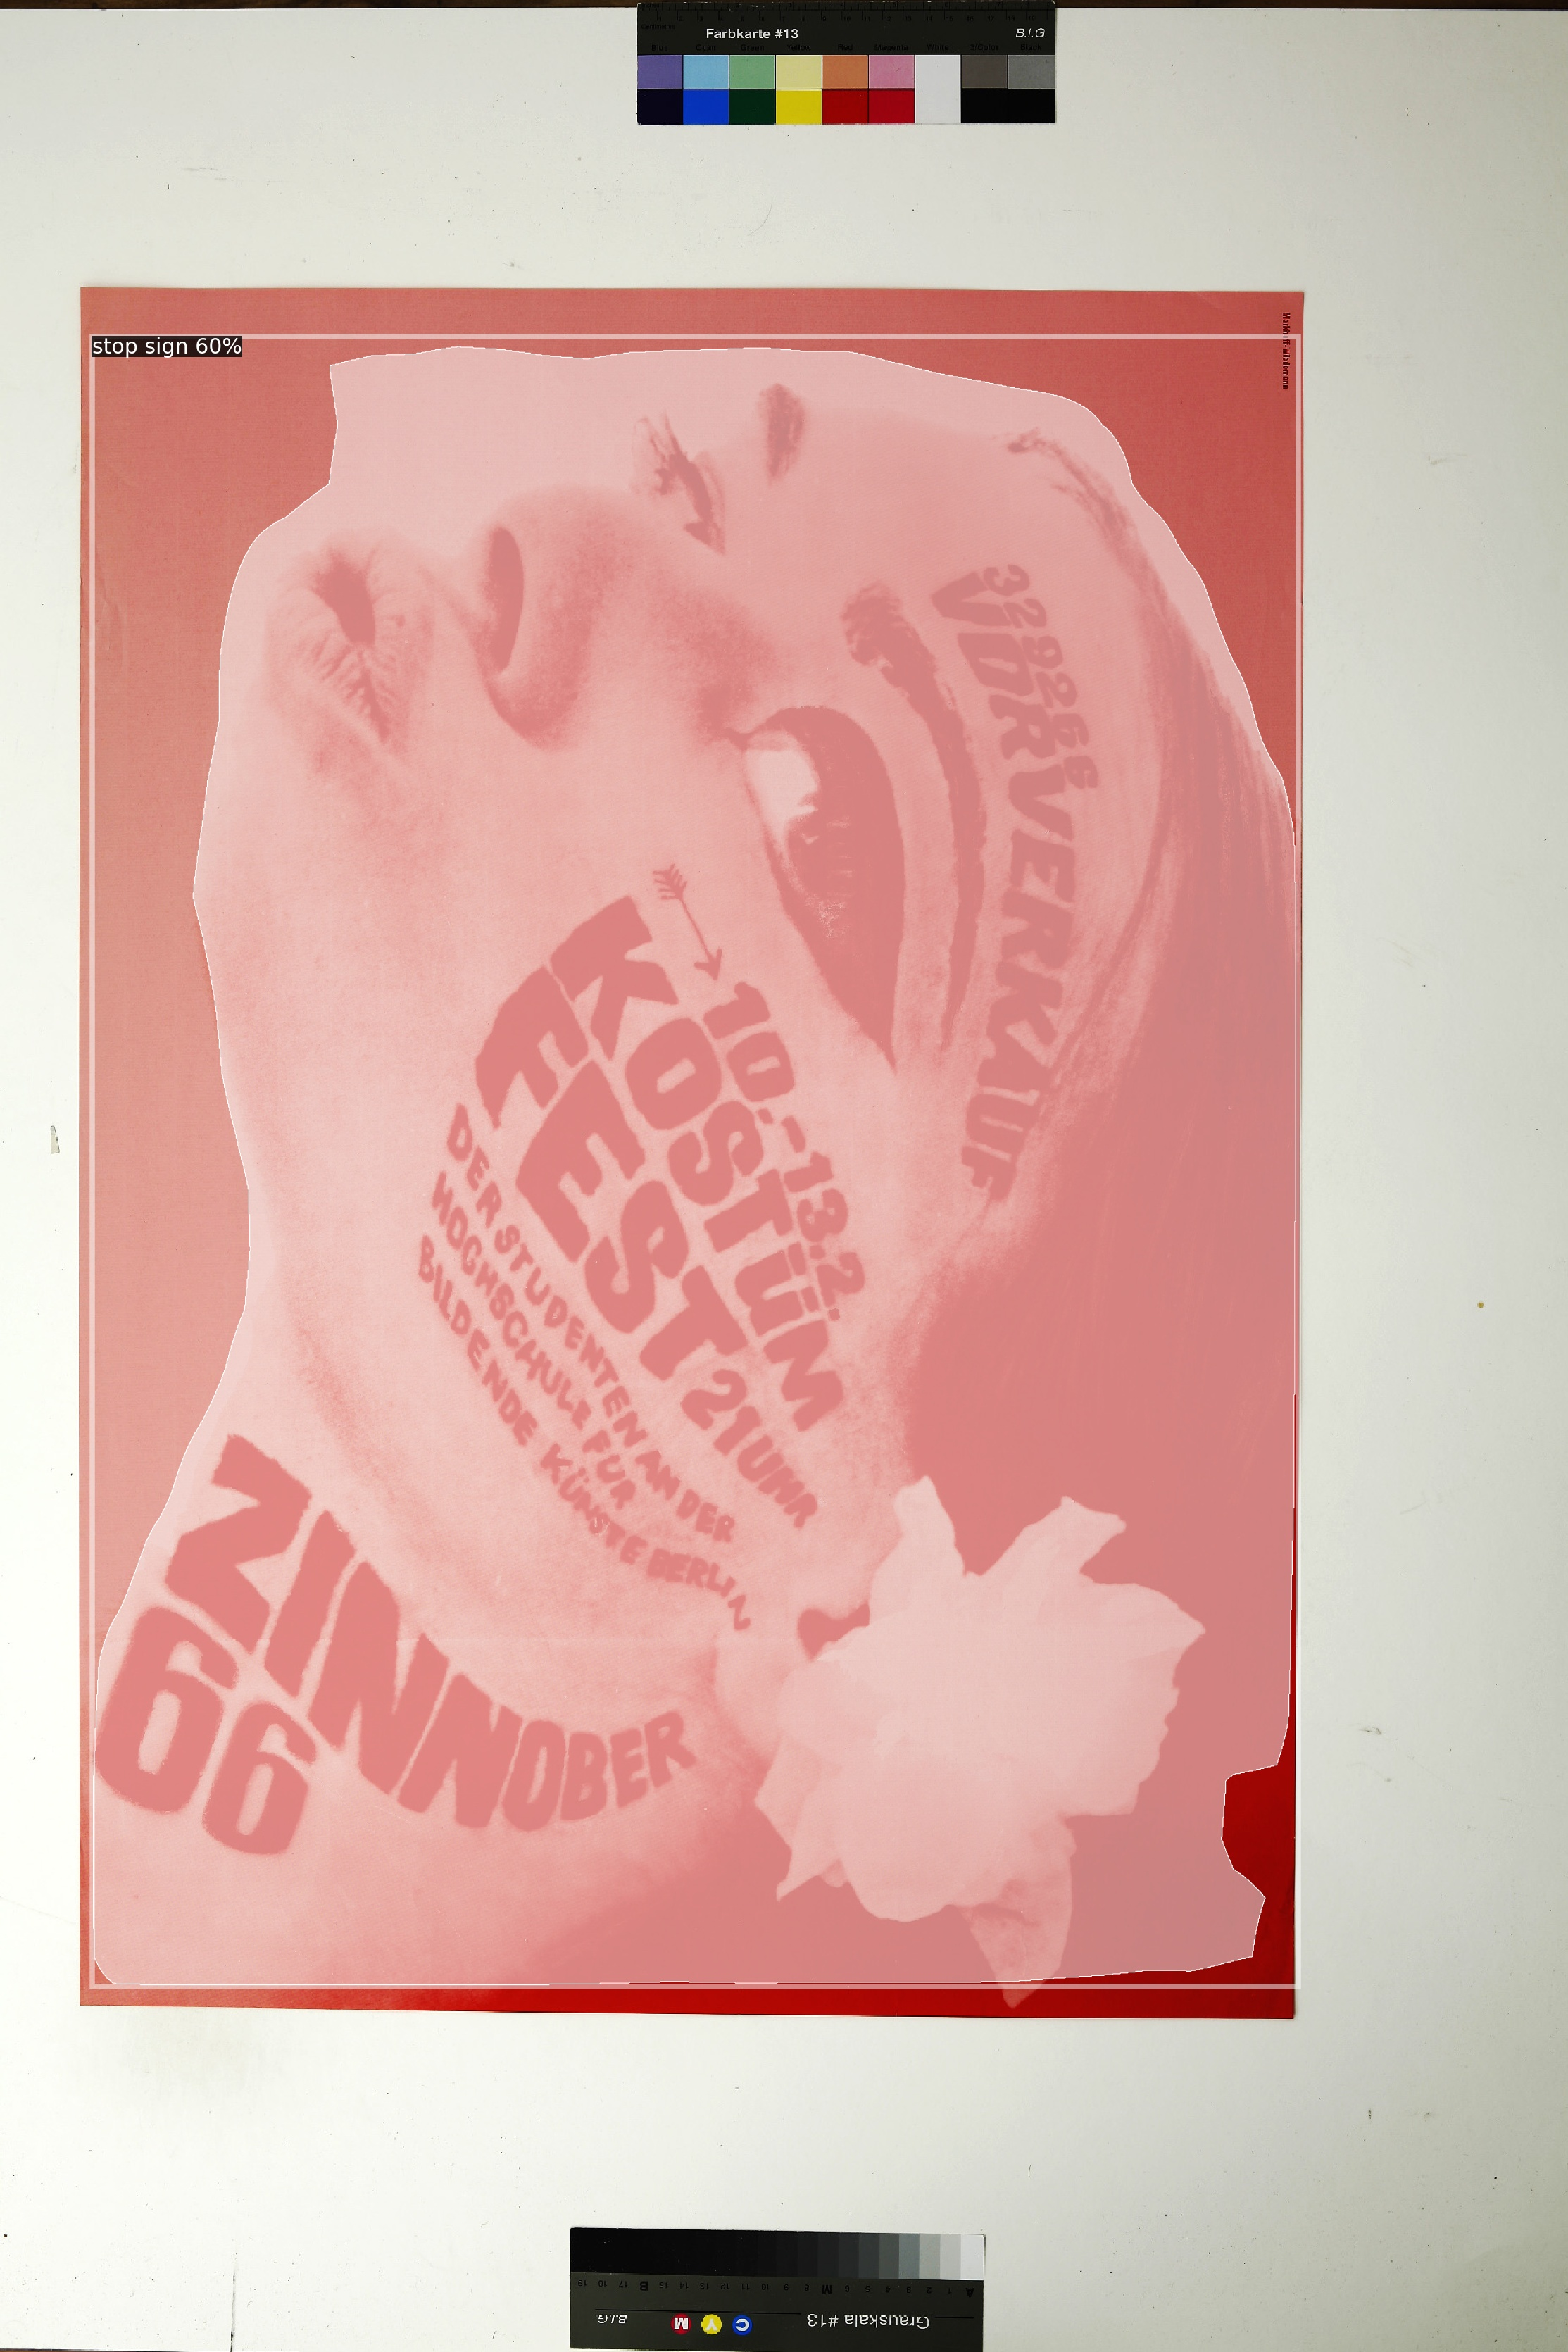
\includegraphics[height=\linewidth]{Abbildung_27_(acht2_068)_with_detections}
	\end{subfigure}
	\caption{Veranstaltungsplakat – Kostümfest, Hochschule für bildende Künste in Berlin, 10.02.-13.02 (acht2\_068); Rechts: Mit Annotationen.}
\end{figure}
\end{landscape}

\newpage
\begin{figure}[ht]
\includegraphics[width=\linewidth]{Abbildung_28_(fünfzehn5_085)}
\centering
\caption{Politisches Plakat – !nein! zur Todesstrafe, amnesty international, ohne Datum (fünfzehn5\_085).}
\end{figure}

\newpage
\begin{figure}[ht]
	\begin{subfigure}[b]{\linewidth}
	\centering
	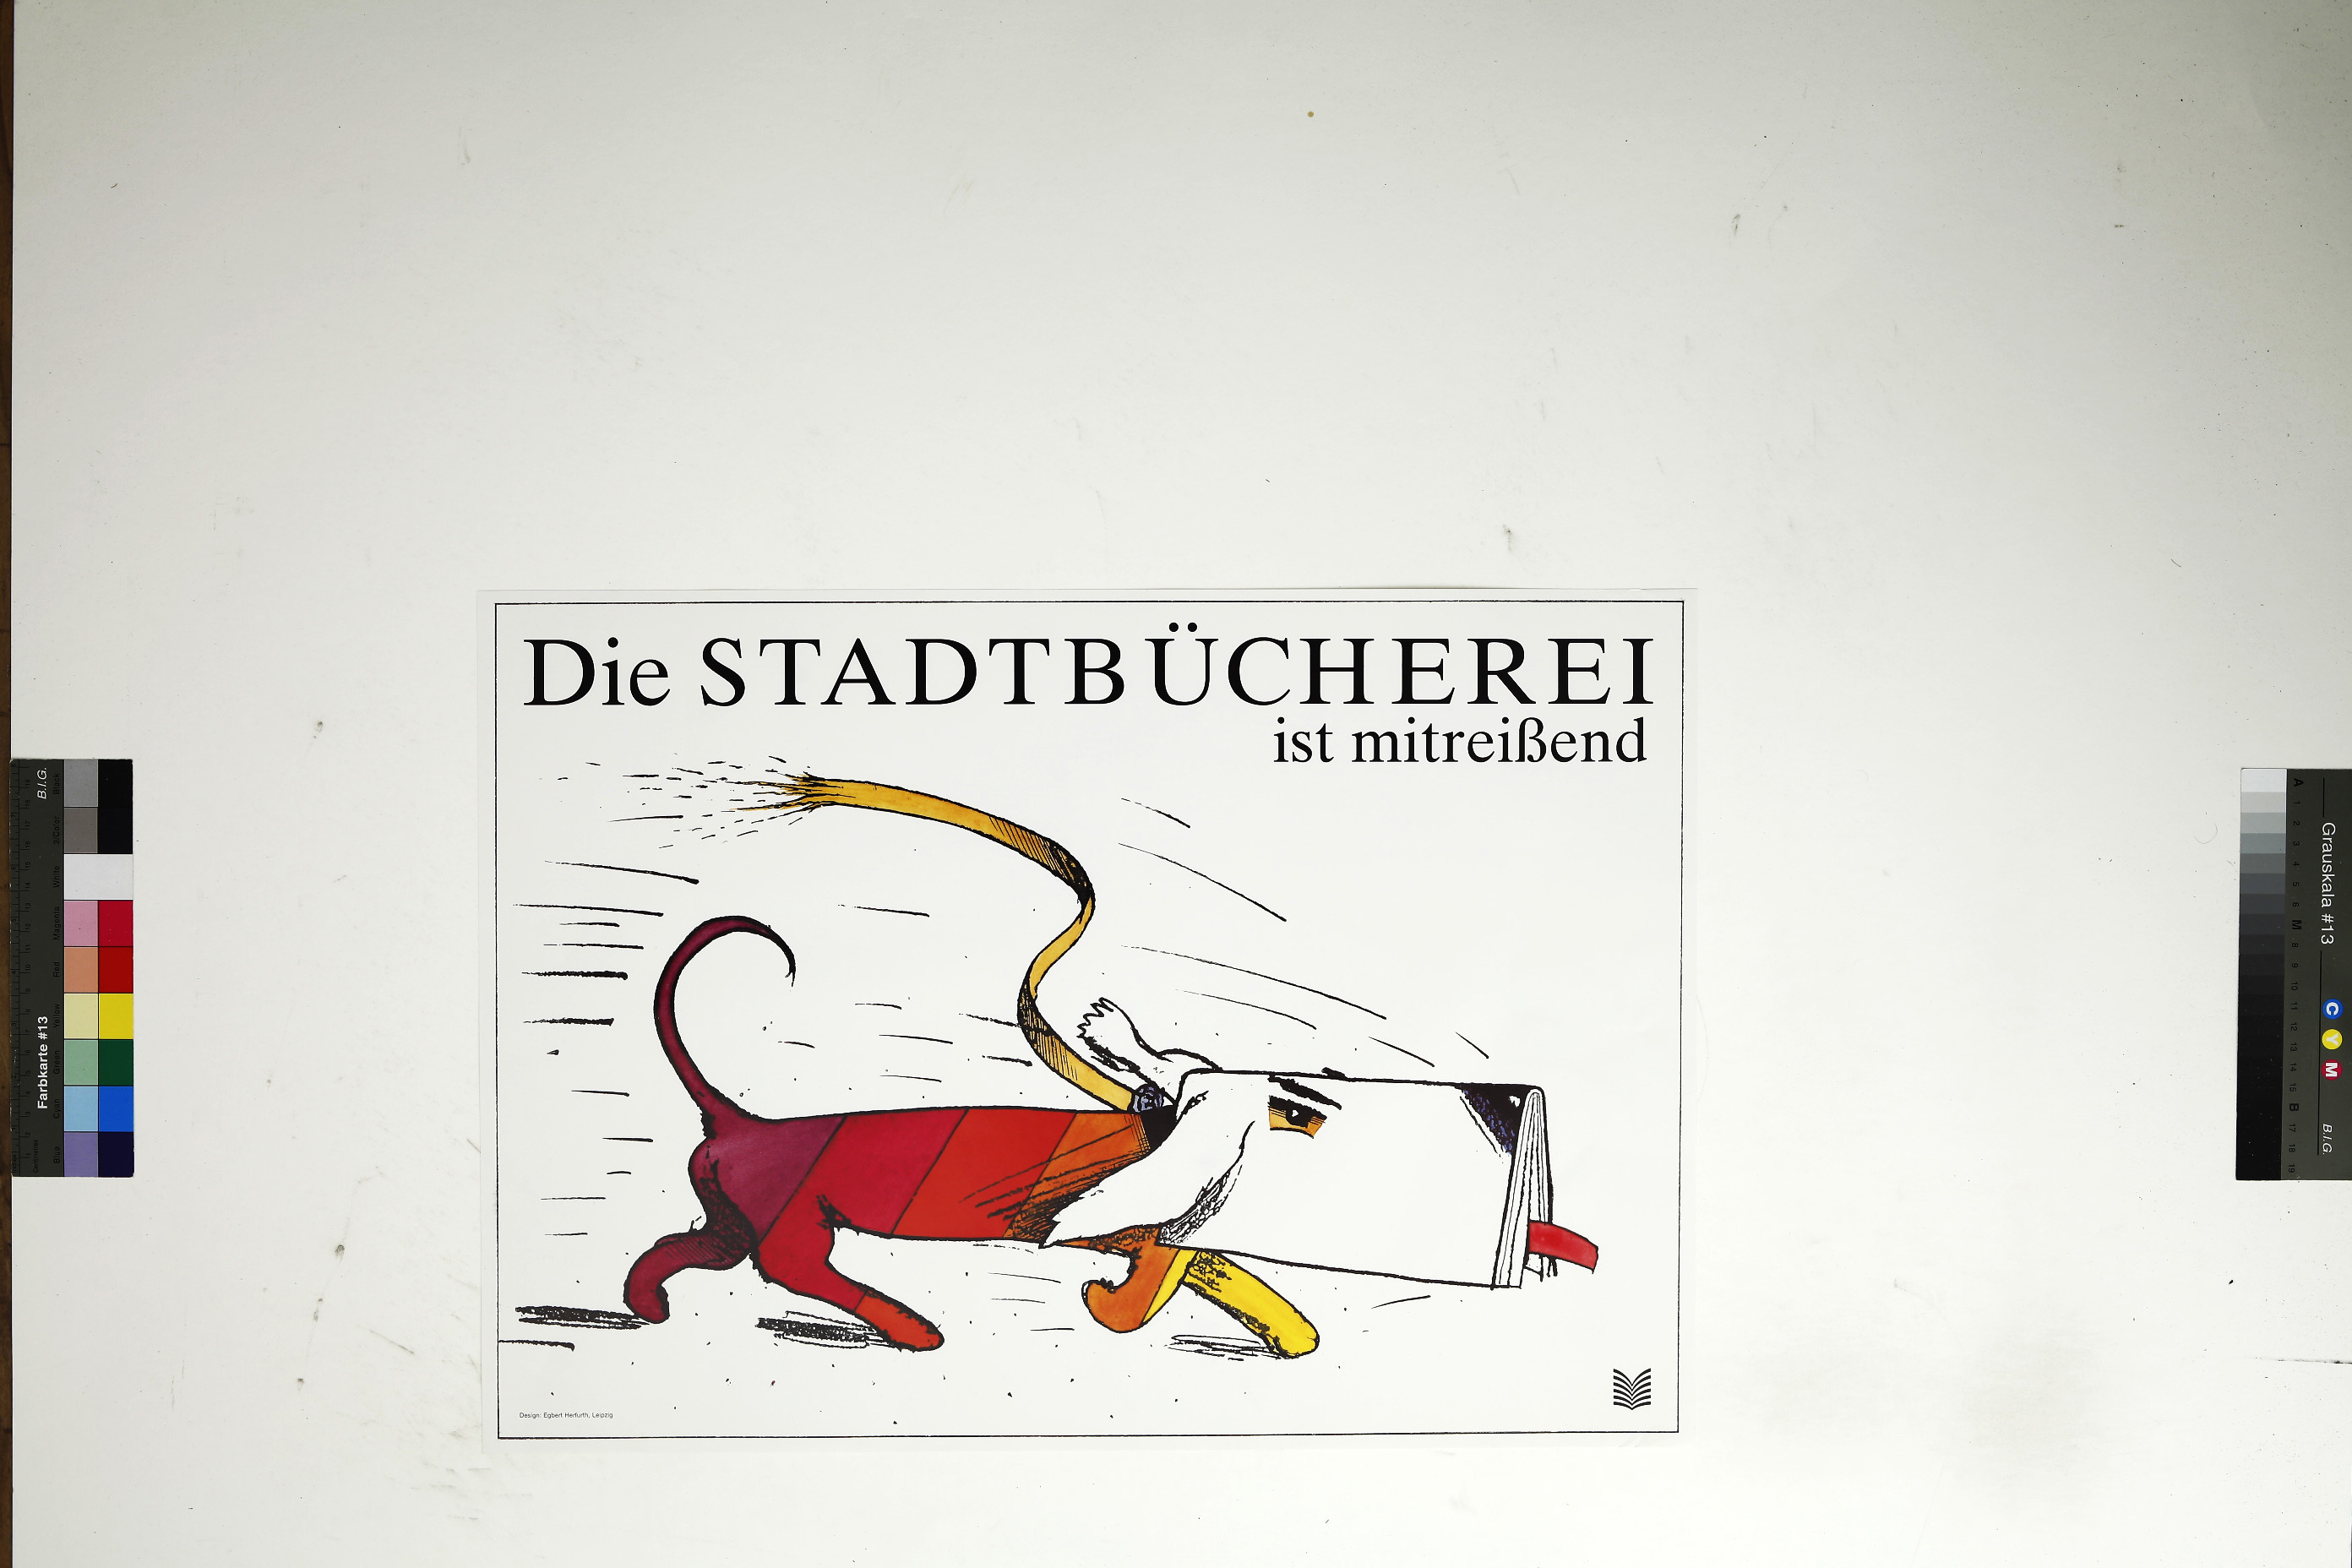
\includegraphics[height=\linewidth, angle=90]{Abbildung_29_(acht1_015)}
	\end{subfigure}
	\begin{subfigure}[b]{\linewidth}
	\centering
	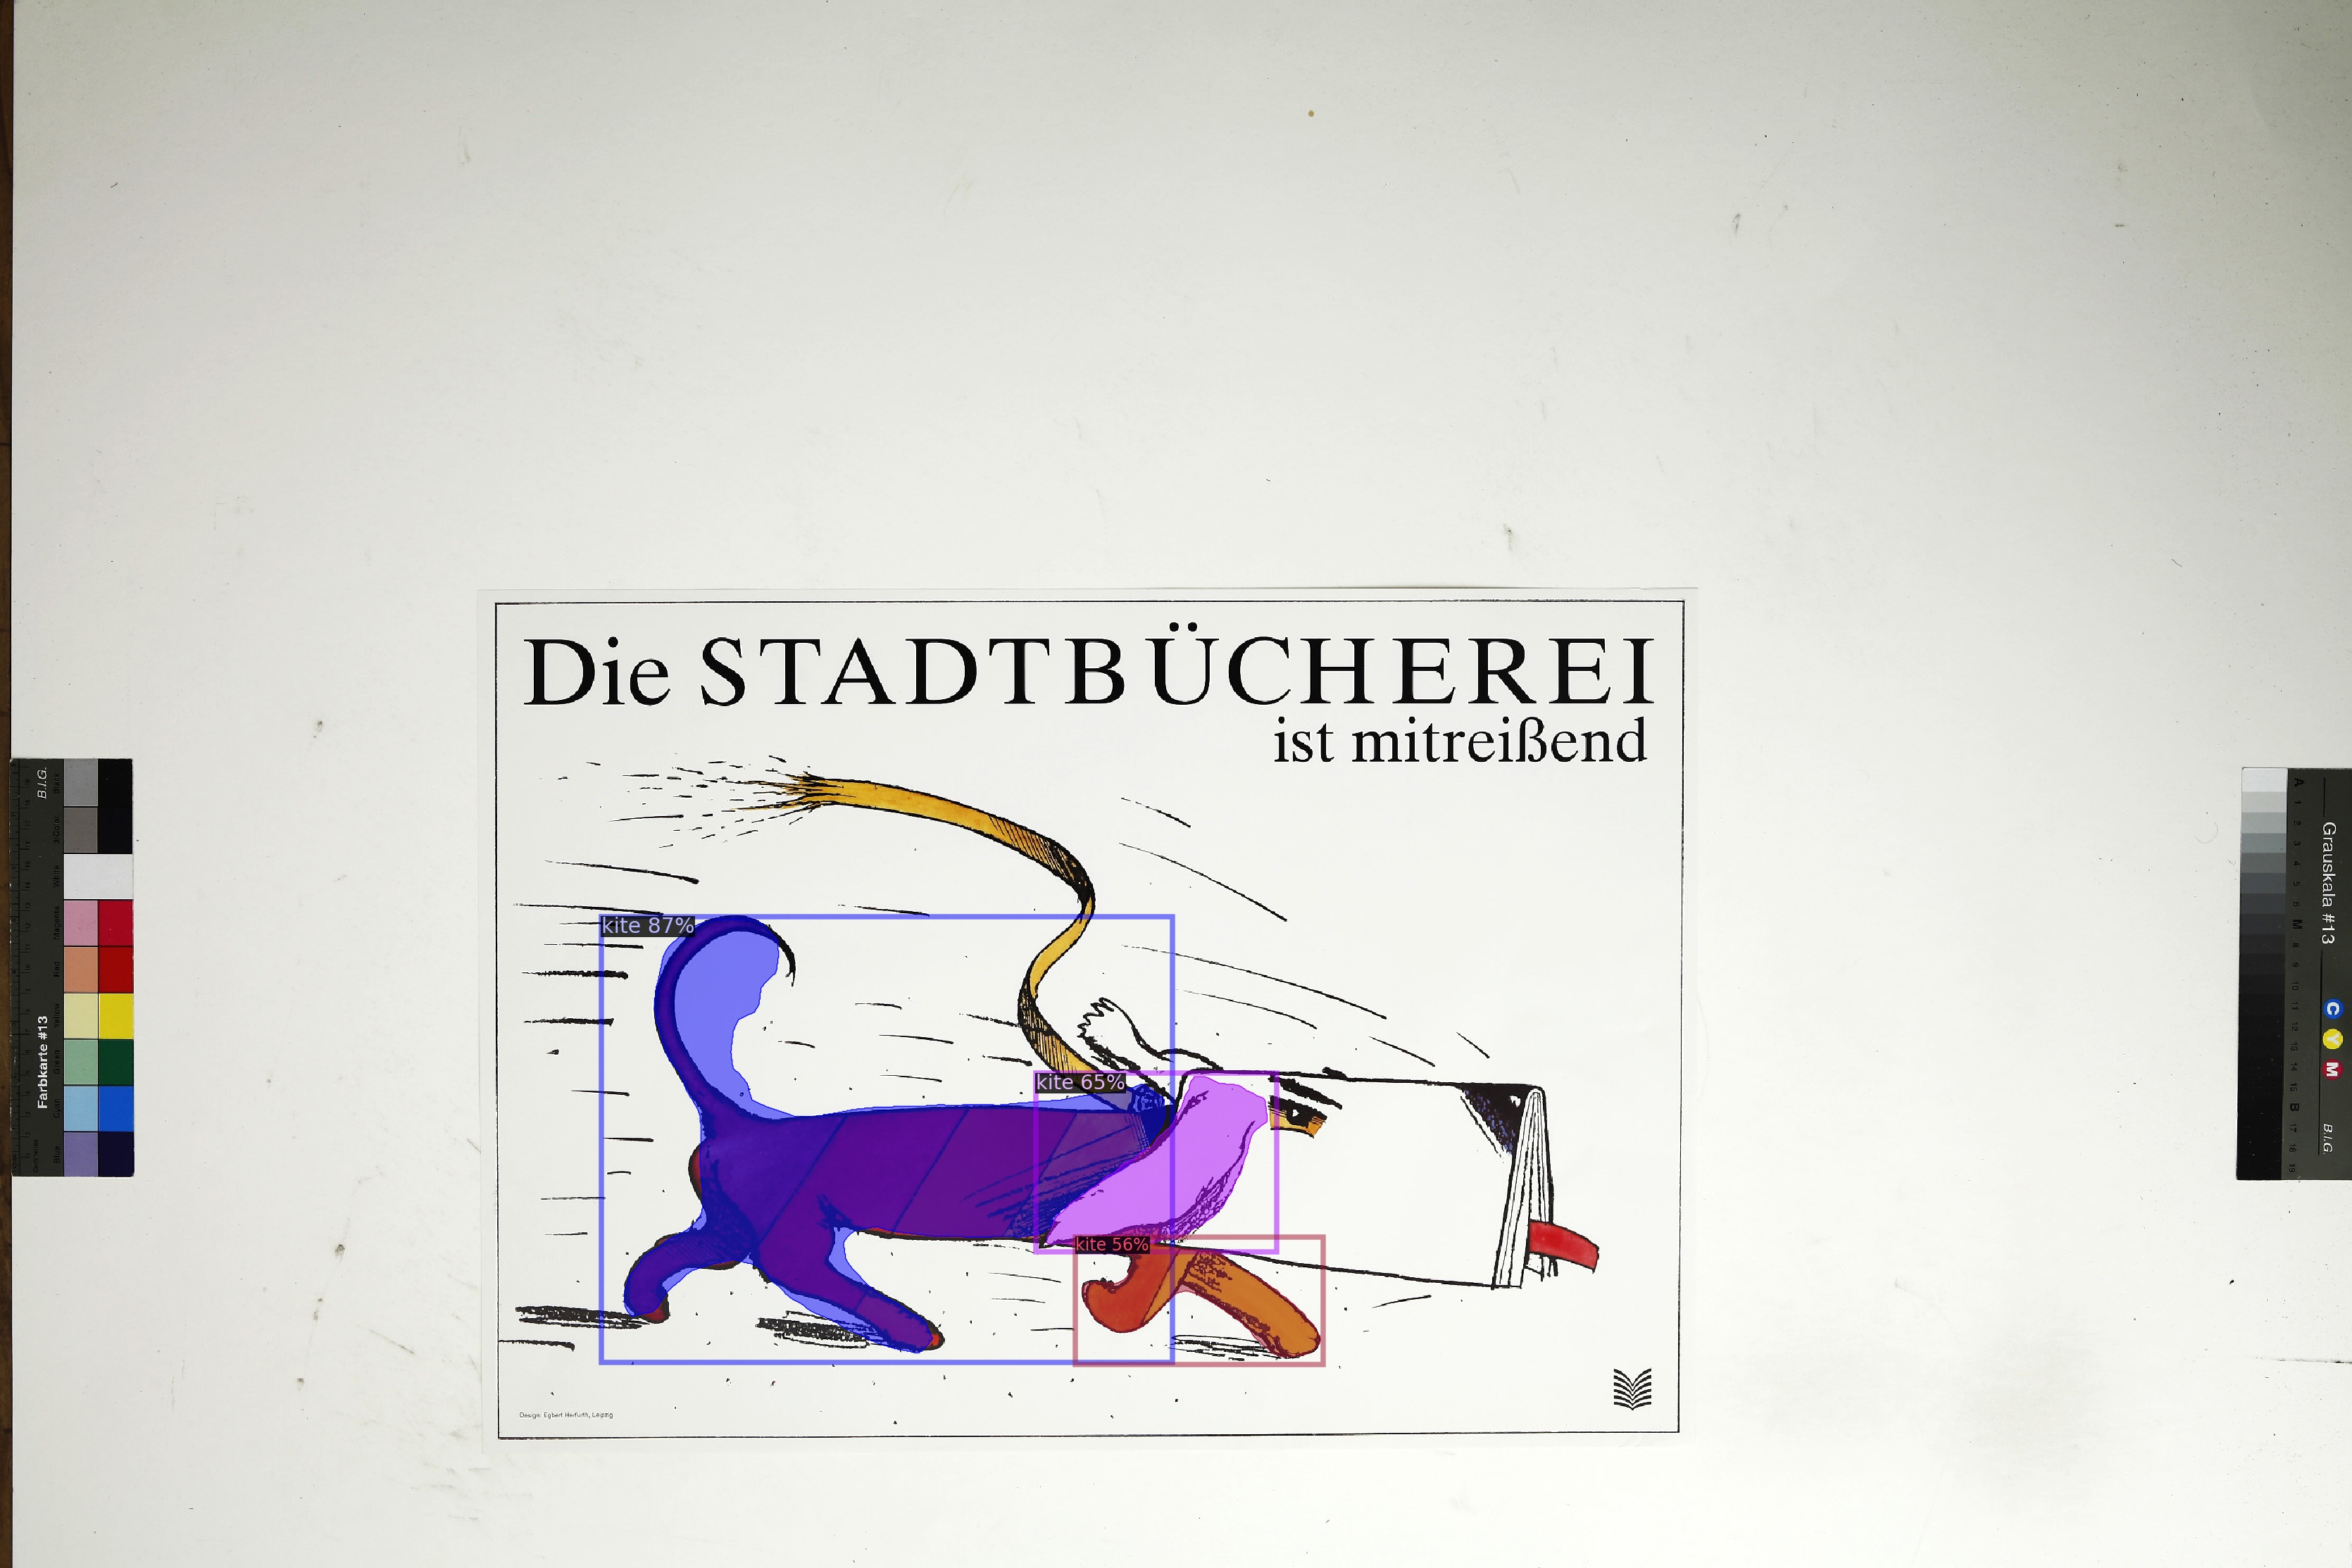
\includegraphics[height=\linewidth, angle=90]{Abbildung_29_(acht1_015)_with_detections}
	\end{subfigure}
	\caption{Werbeplakat – Die Stadtbücherei ist mitreißend, ohne Datum (acht1\_015); Unten: Mit Annotationen.}
\end{figure}

\newpage
\begin{landscape}
\begin{figure}[ht]
	\begin{subfigure}[b]{0.5\linewidth}
	\centering
	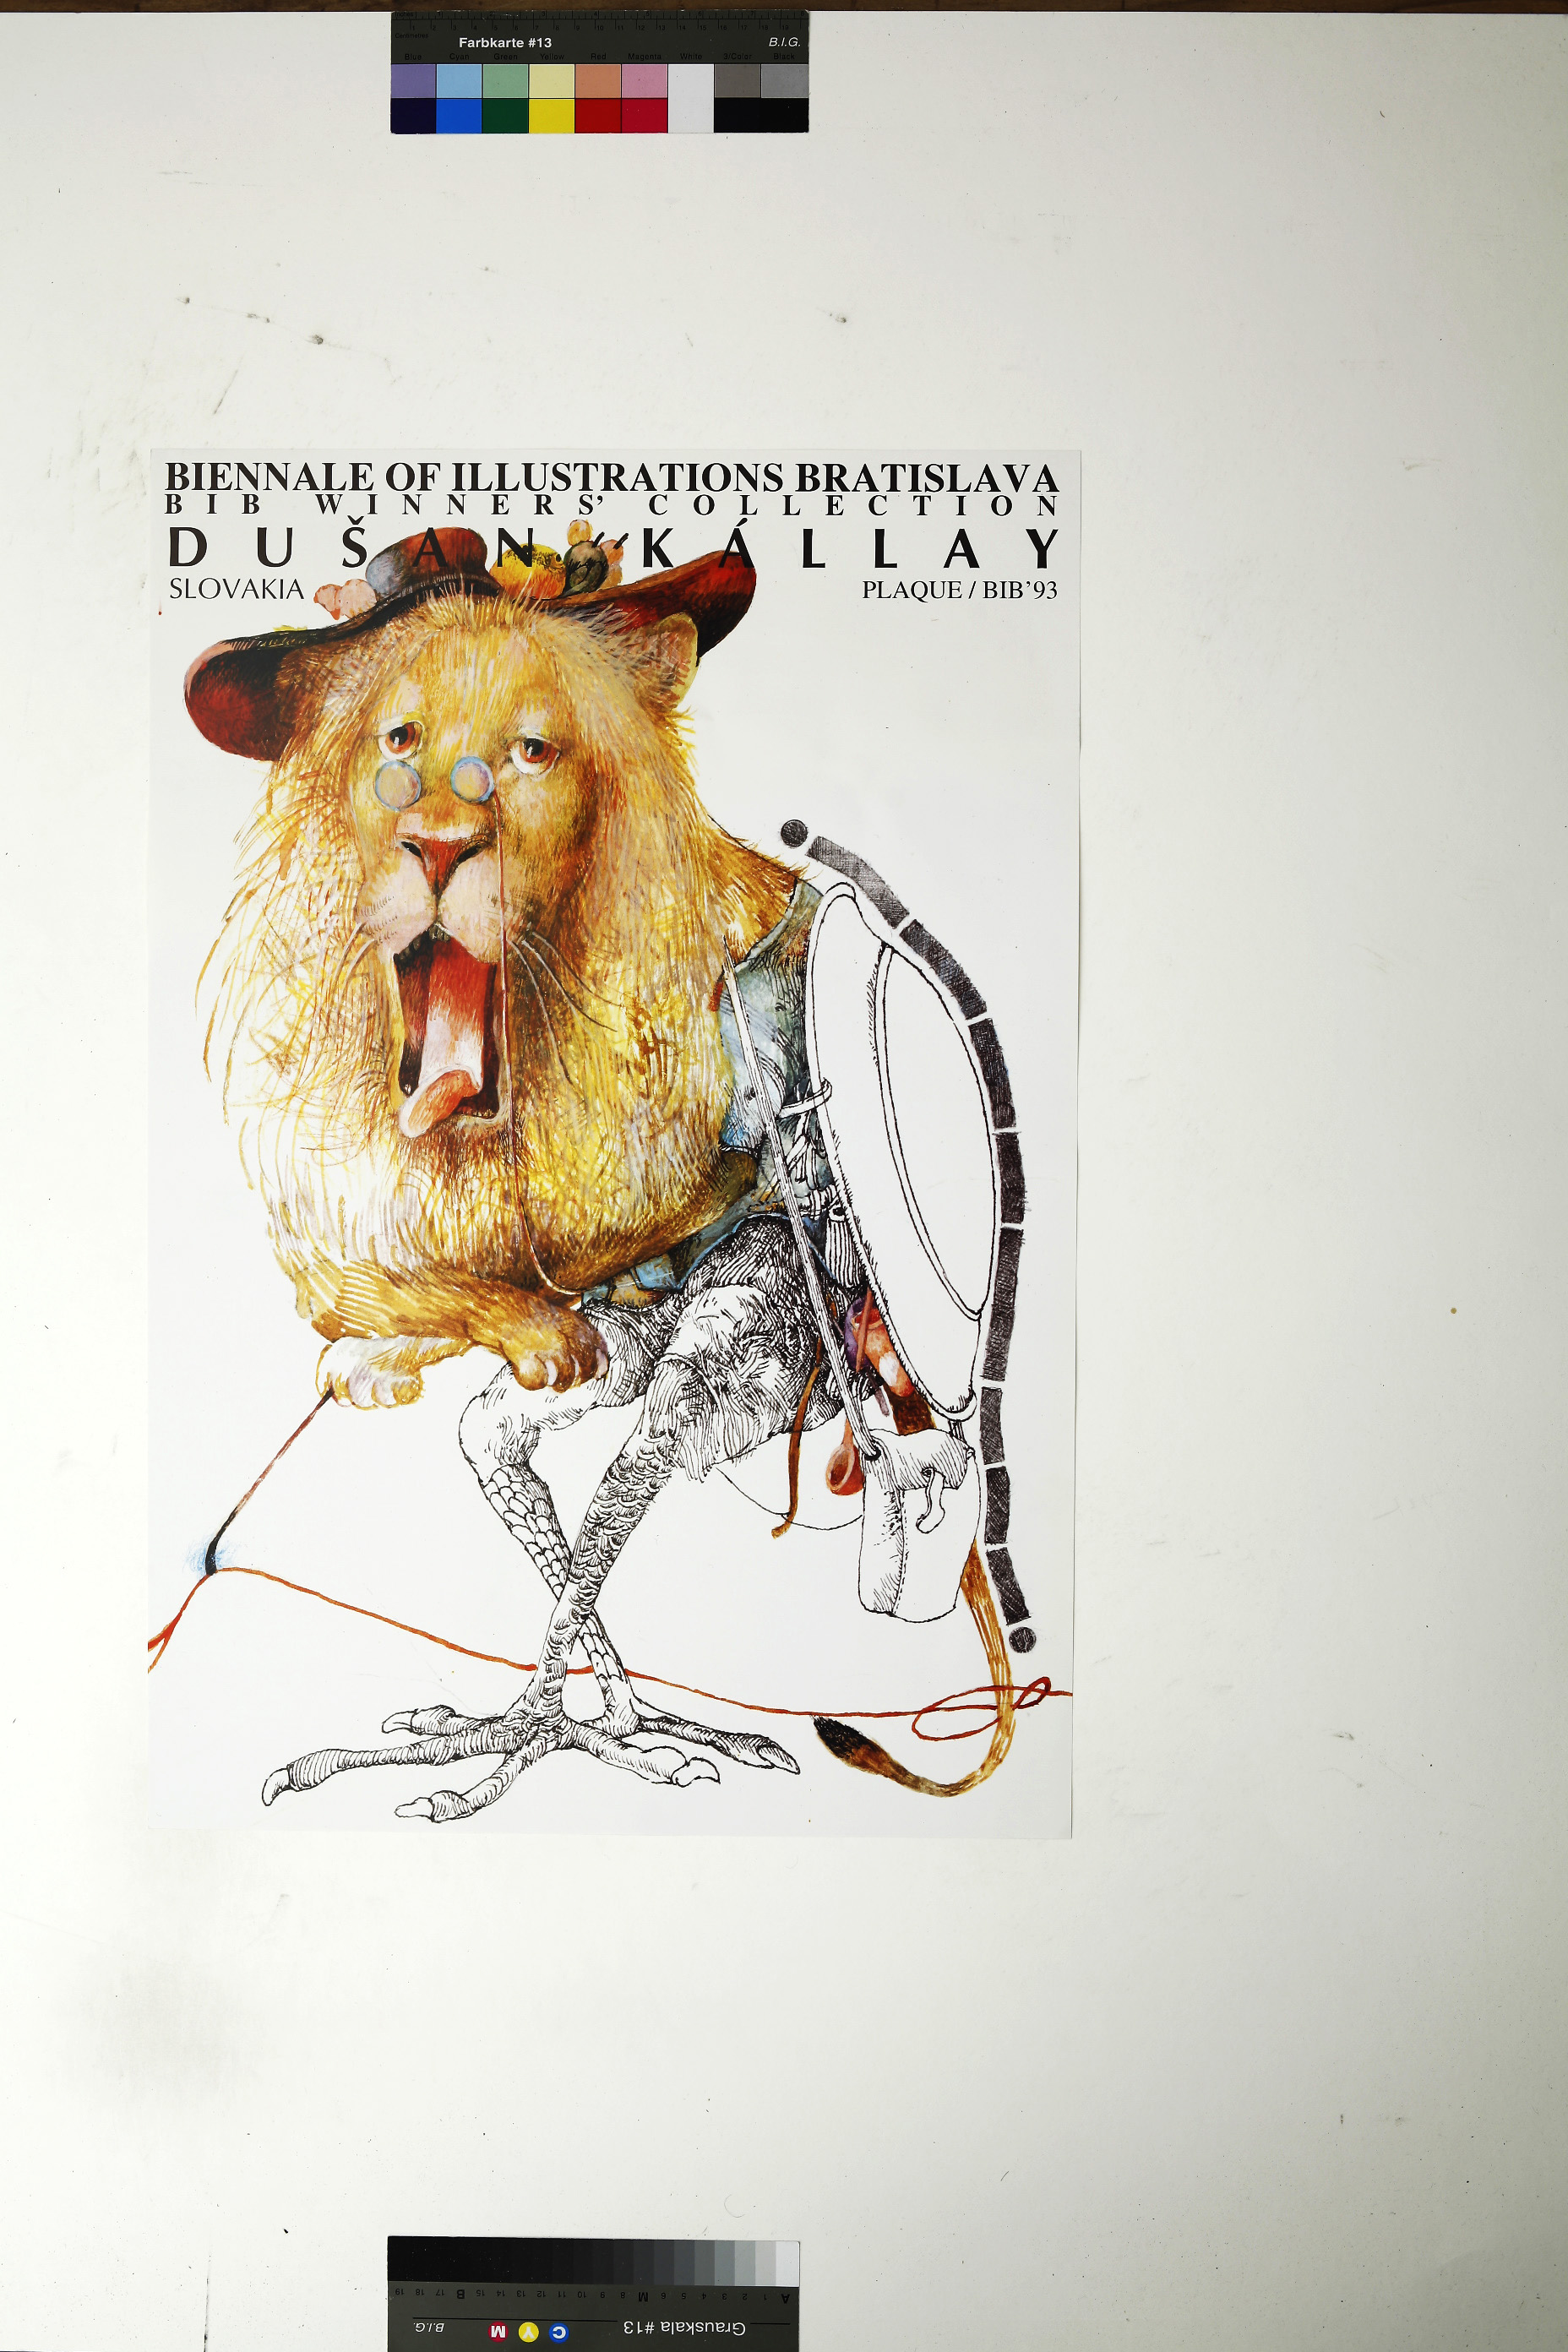
\includegraphics[height=\linewidth]{Abbildung_30_(acht1_023)}
	\end{subfigure}
	\begin{subfigure}[b]{0.5\linewidth}
	\centering
	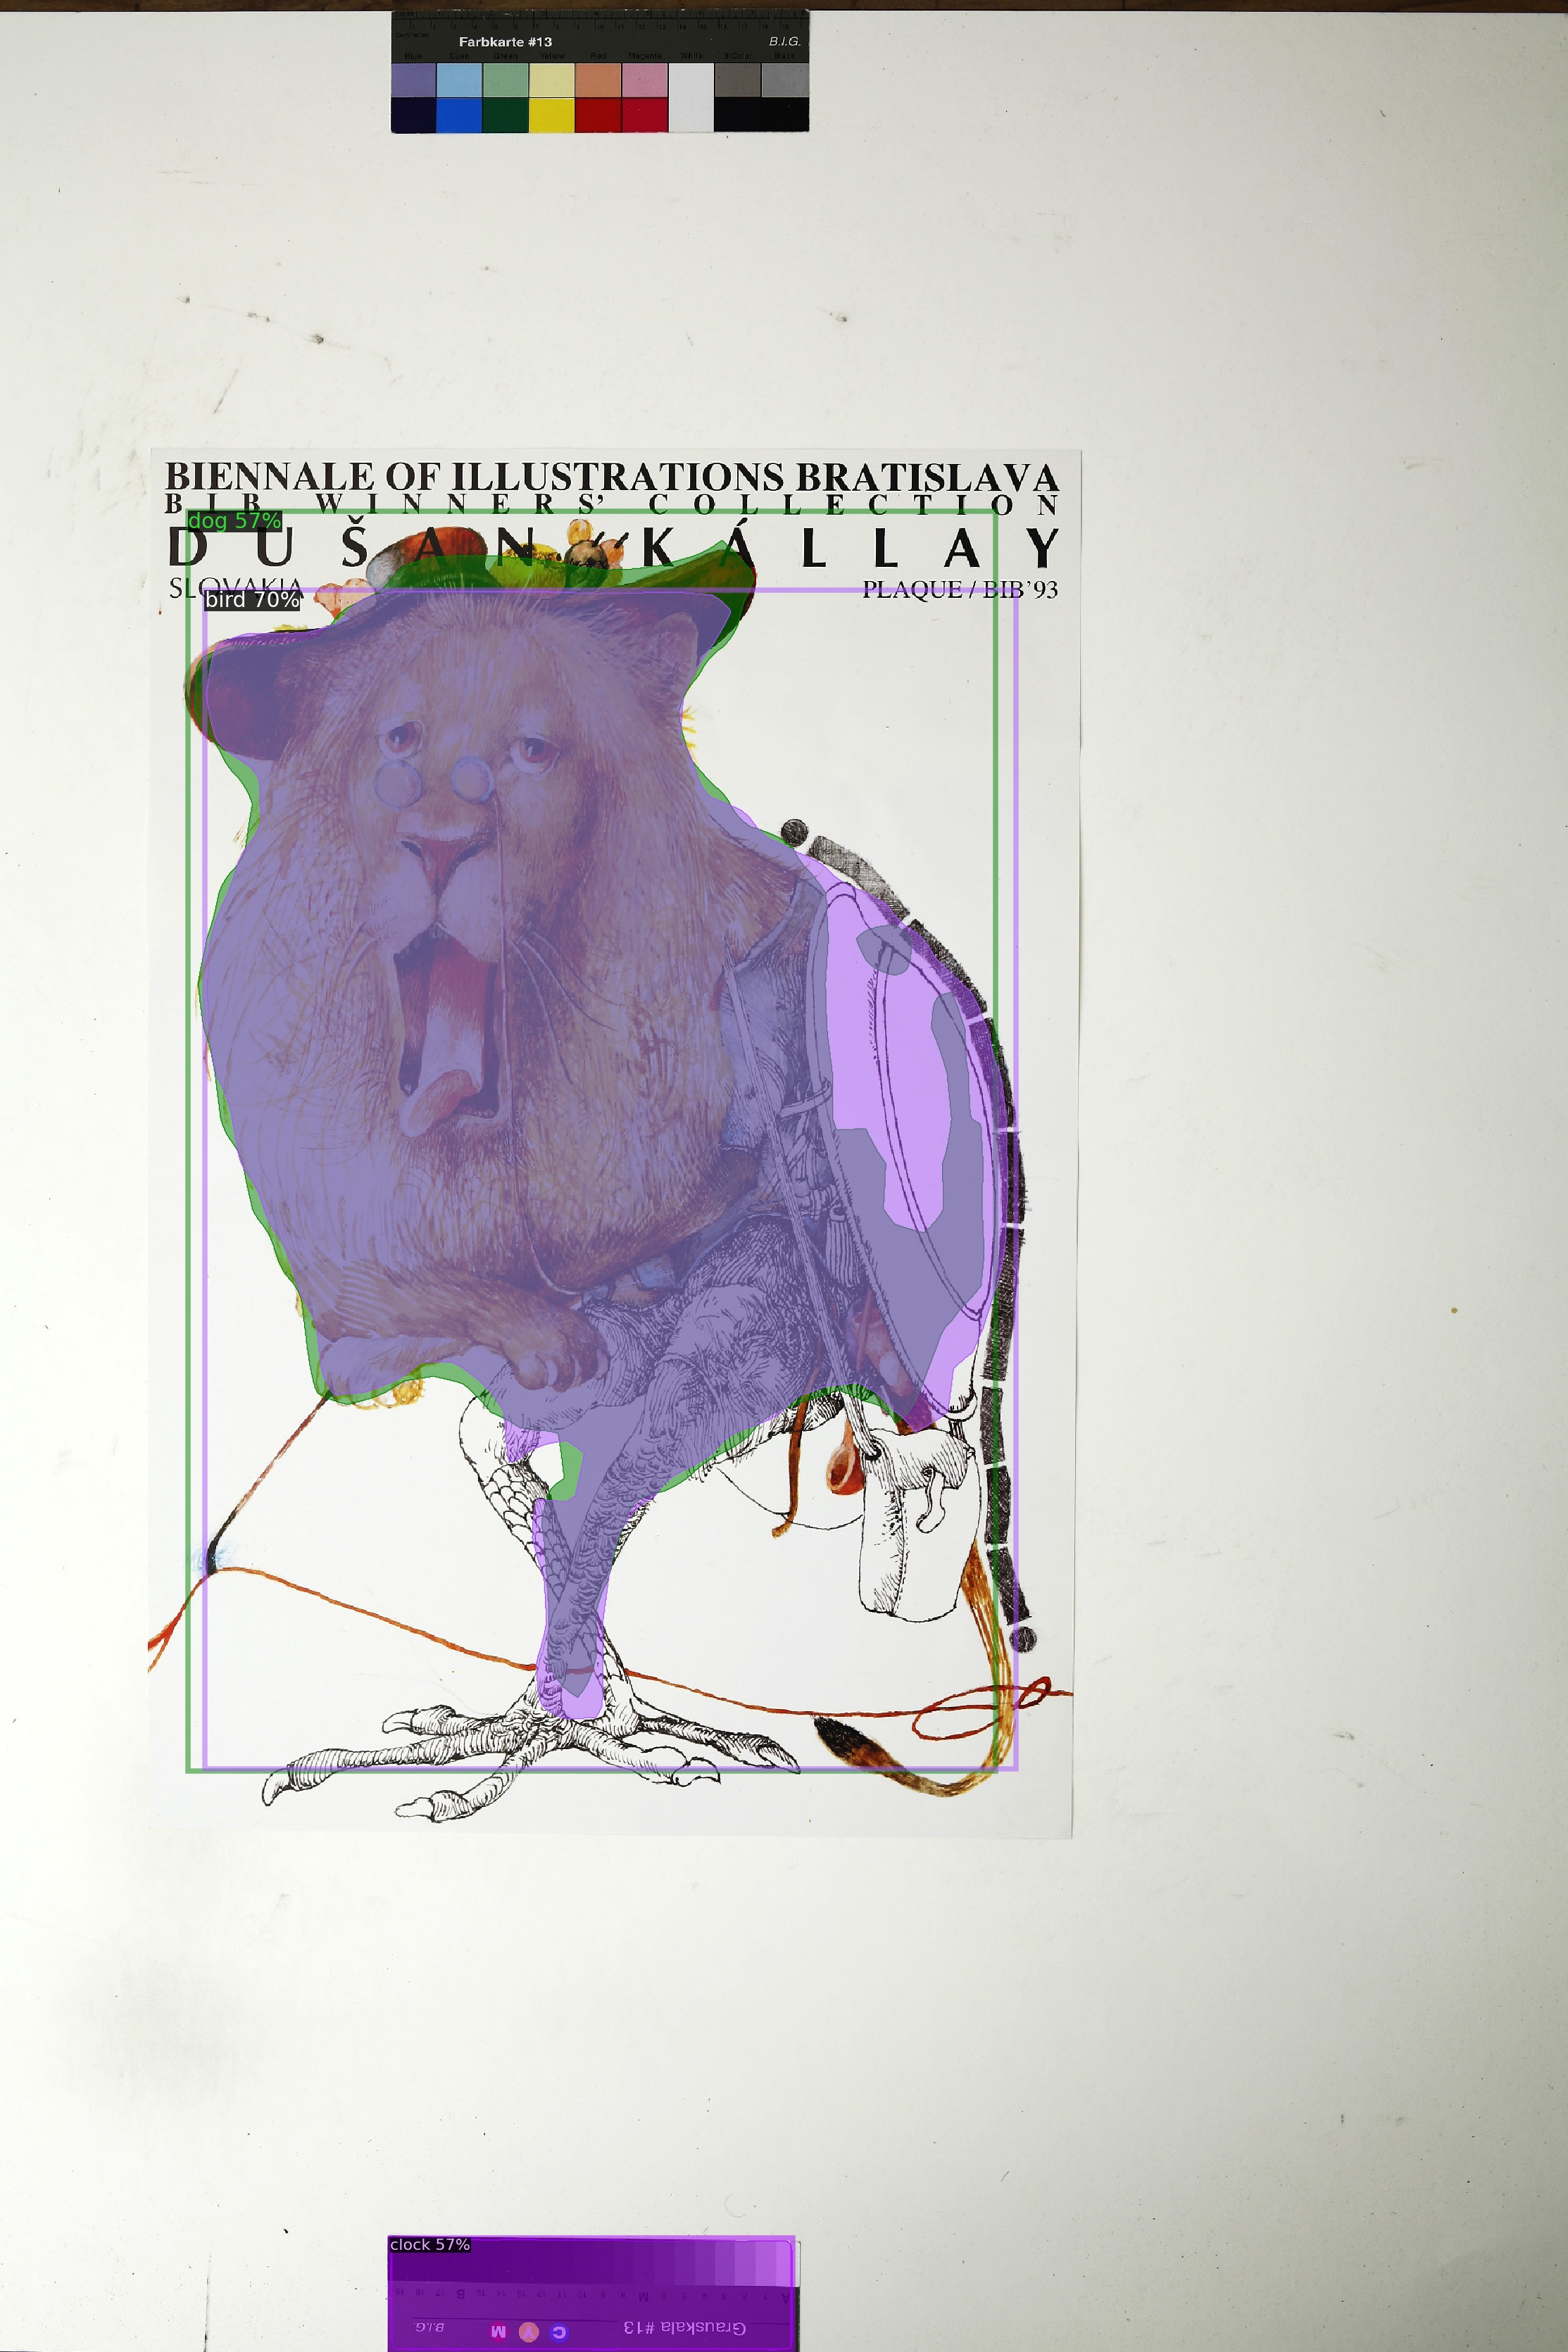
\includegraphics[height=\linewidth]{Abbildung_30_(acht1_023)_with_detections}
	\end{subfigure}
	\caption{Veranstaltungsplakat – Biennale of Illustrations Bratislava, 1993 (acht1\_023); Rechts: Mit Annotationen.}
\end{figure}
\end{landscape}

\newpage
\begin{landscape}
\begin{figure}[ht]
	\begin{subfigure}[b]{0.5\linewidth}
	\centering
	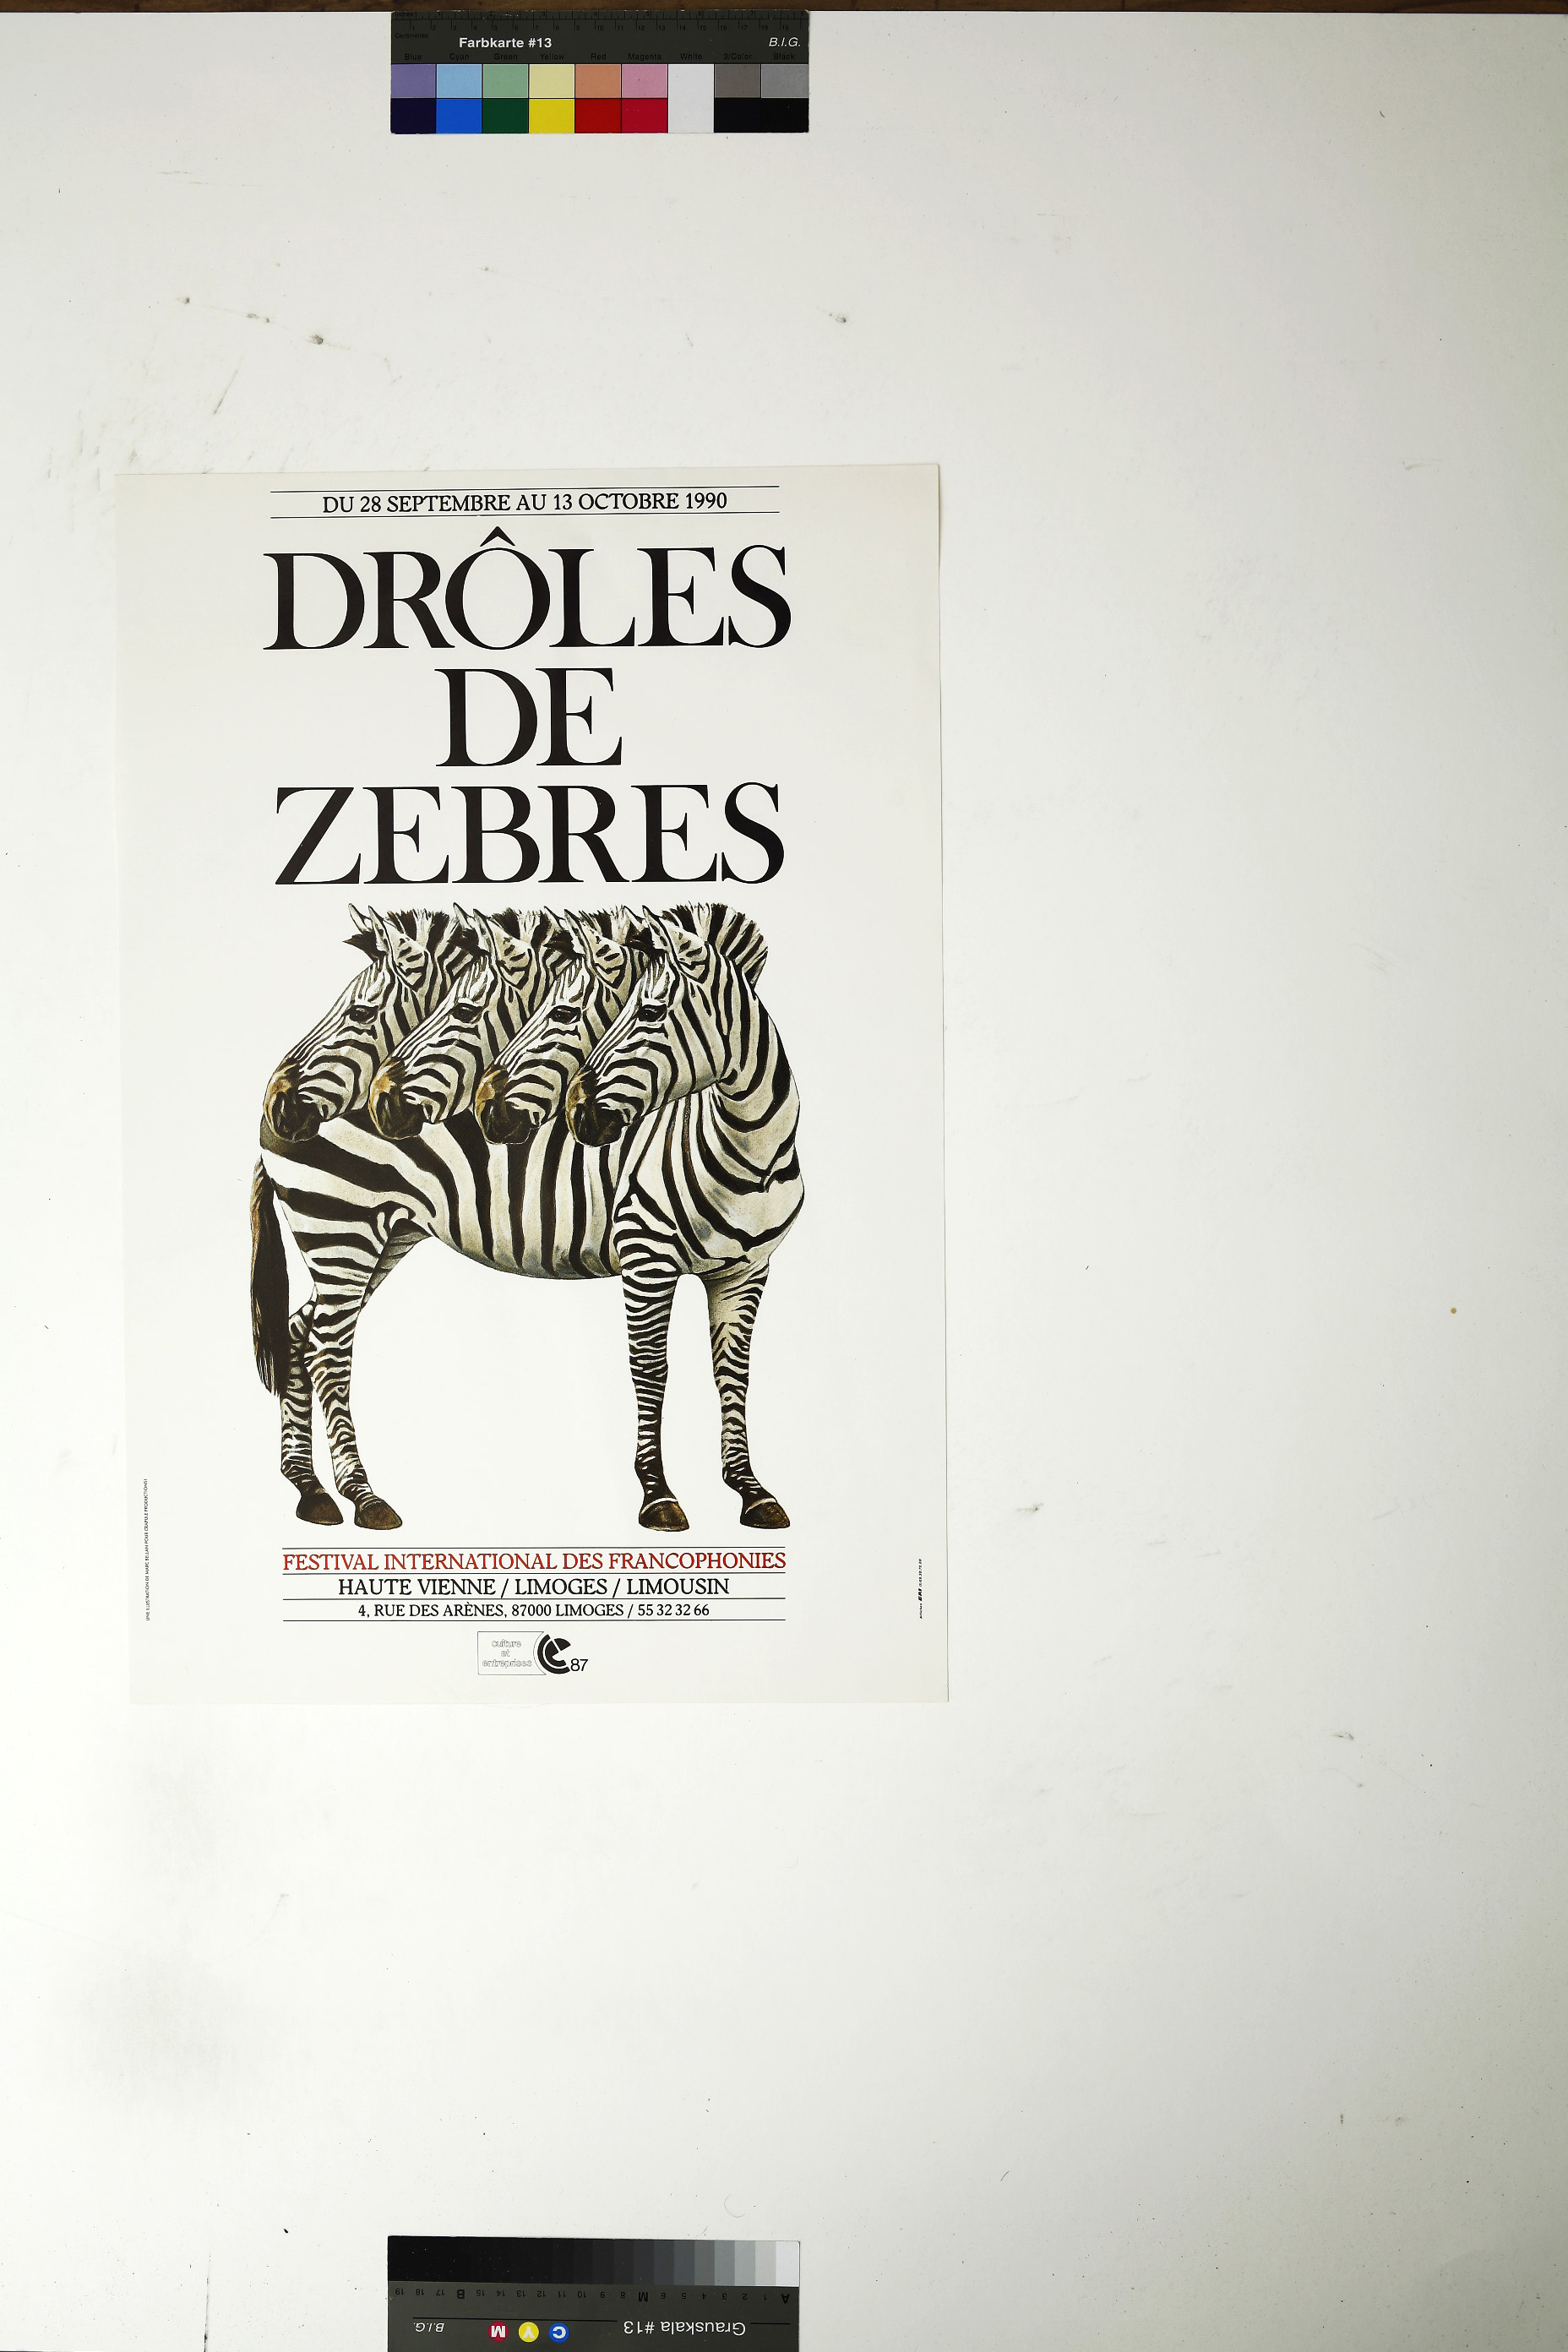
\includegraphics[height=\linewidth]{Abbildung_31_(acht1_016)}
	\end{subfigure}
	\begin{subfigure}[b]{0.5\linewidth}
	\centering
	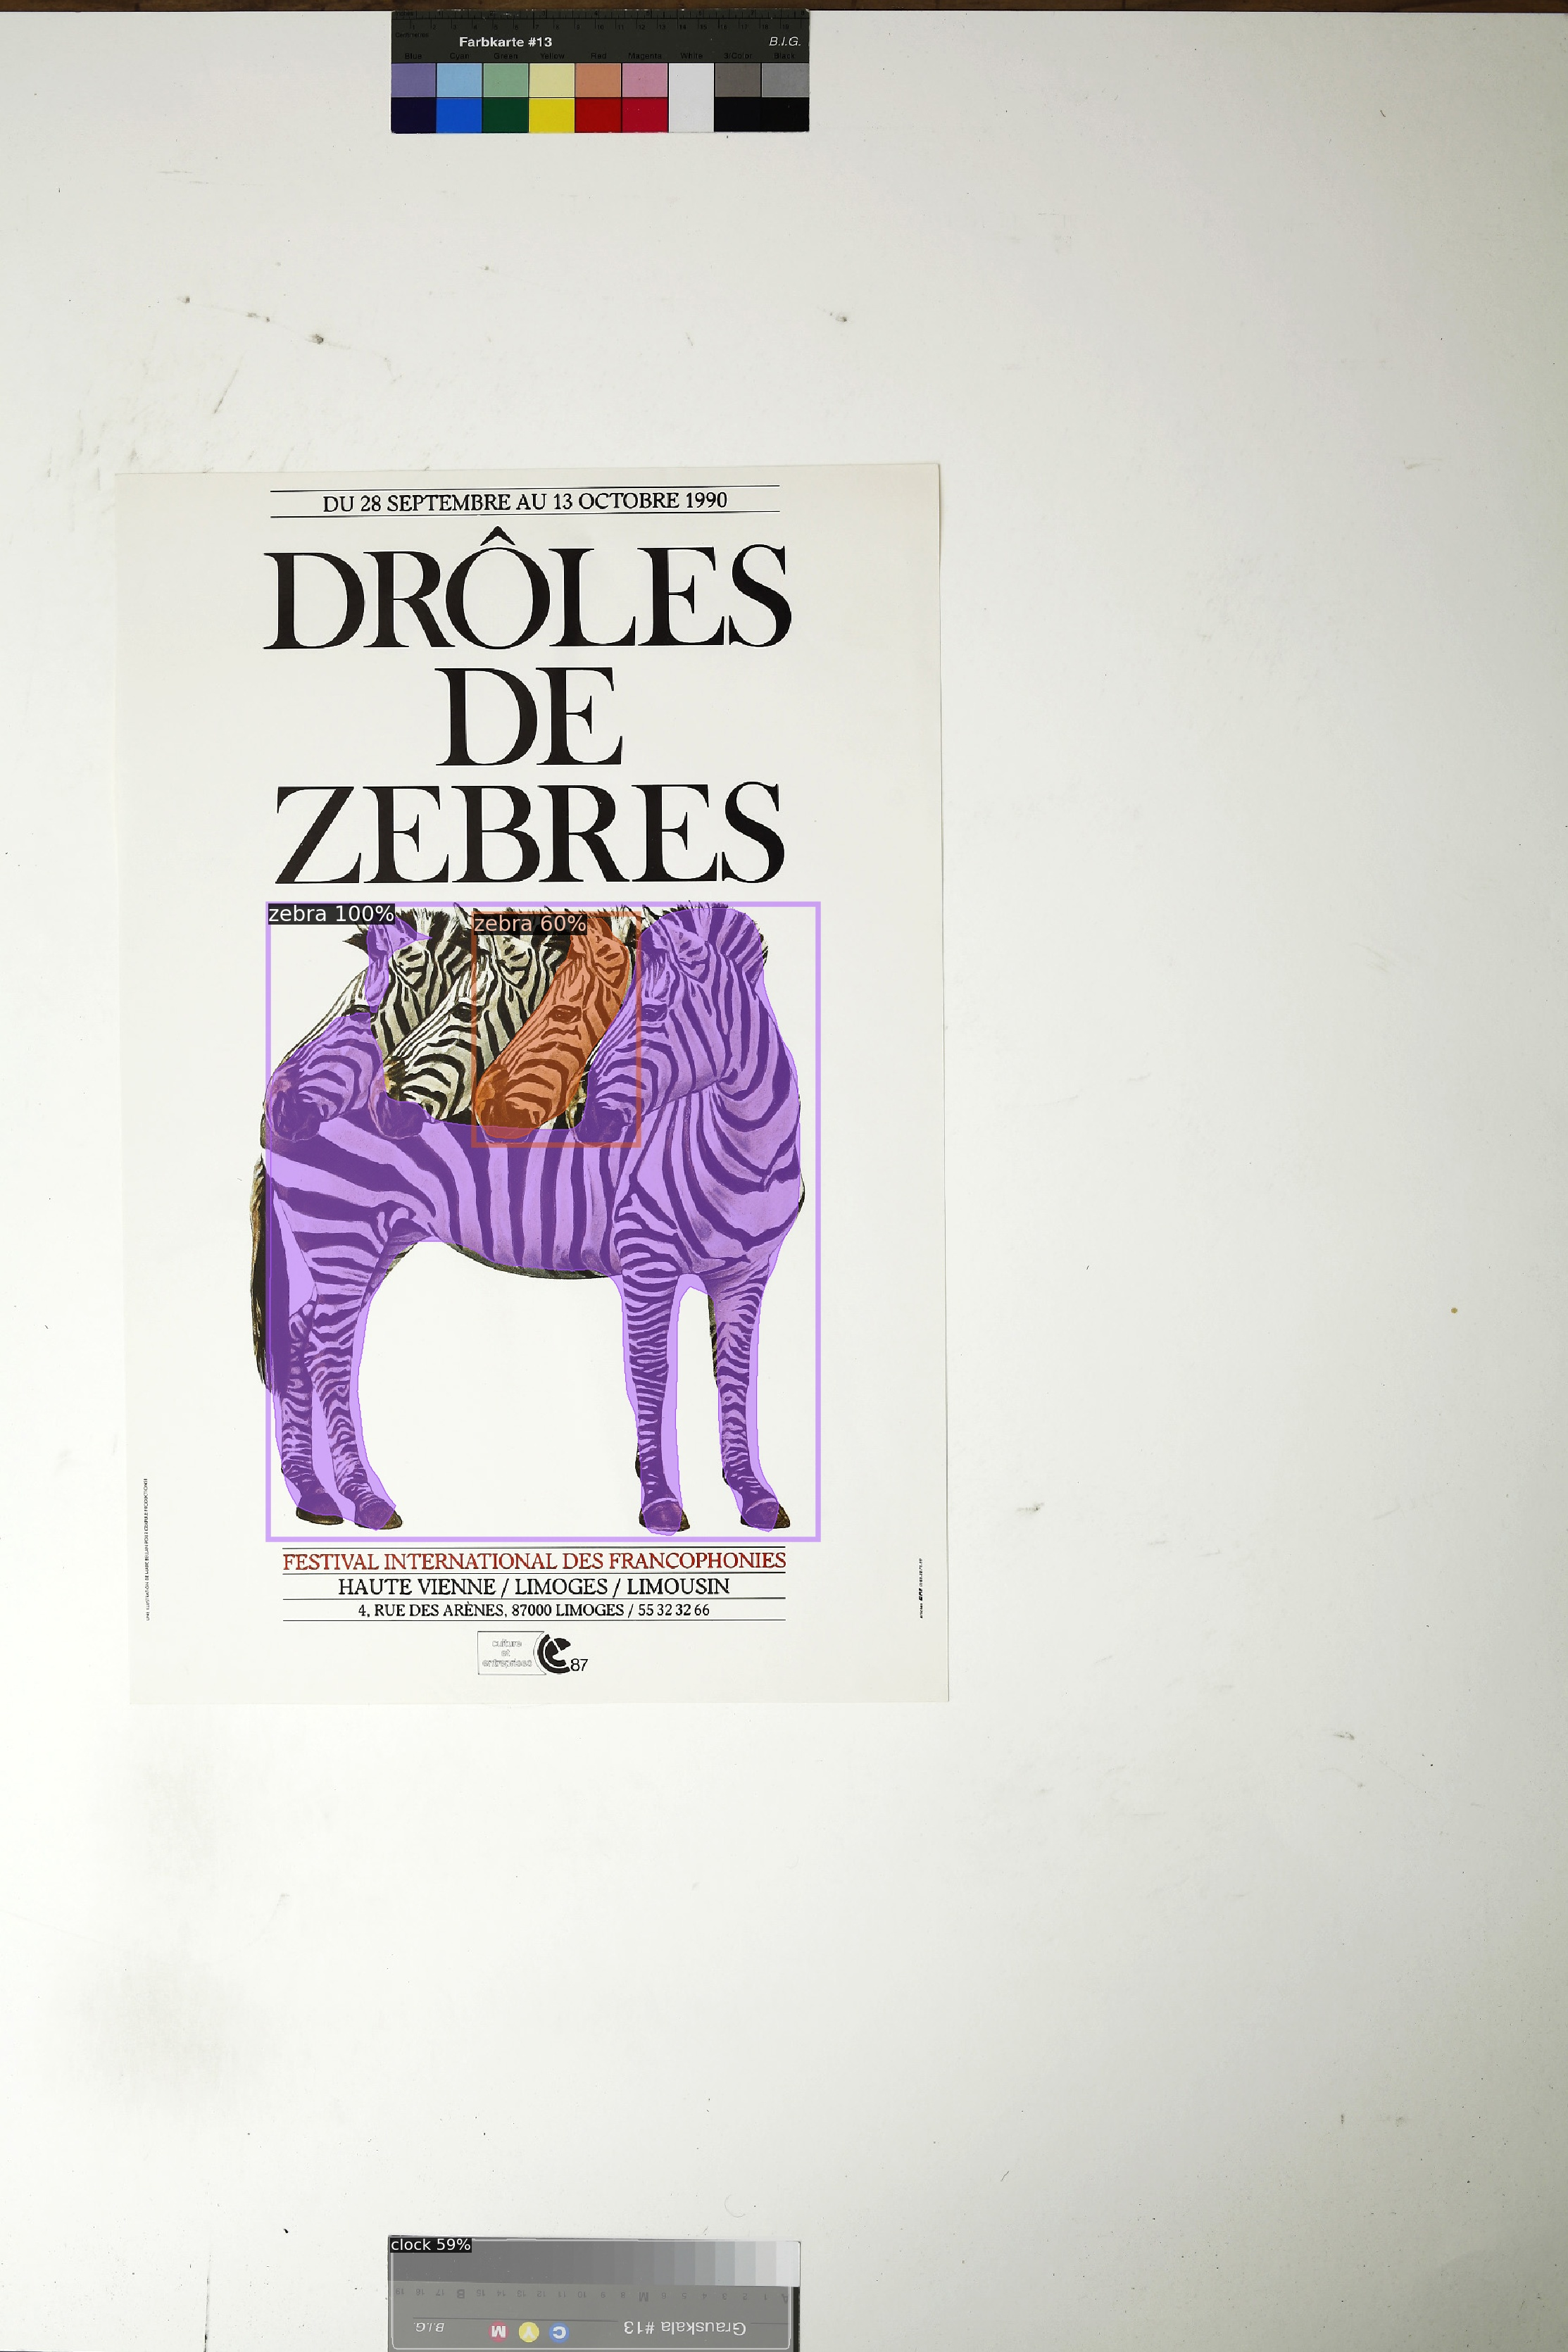
\includegraphics[height=\linewidth]{Abbildung_31_(acht1_016)_with_detections}
	\end{subfigure}
	\caption{Veranstaltungsplakat – Festival International de Francophonies, Haute Vienne, 28.09.1990-13.10.1990 (acht1\_016); Rechts: Mit Annotationen.}
\end{figure}
\end{landscape}

\newpage
\begin{figure}[ht]
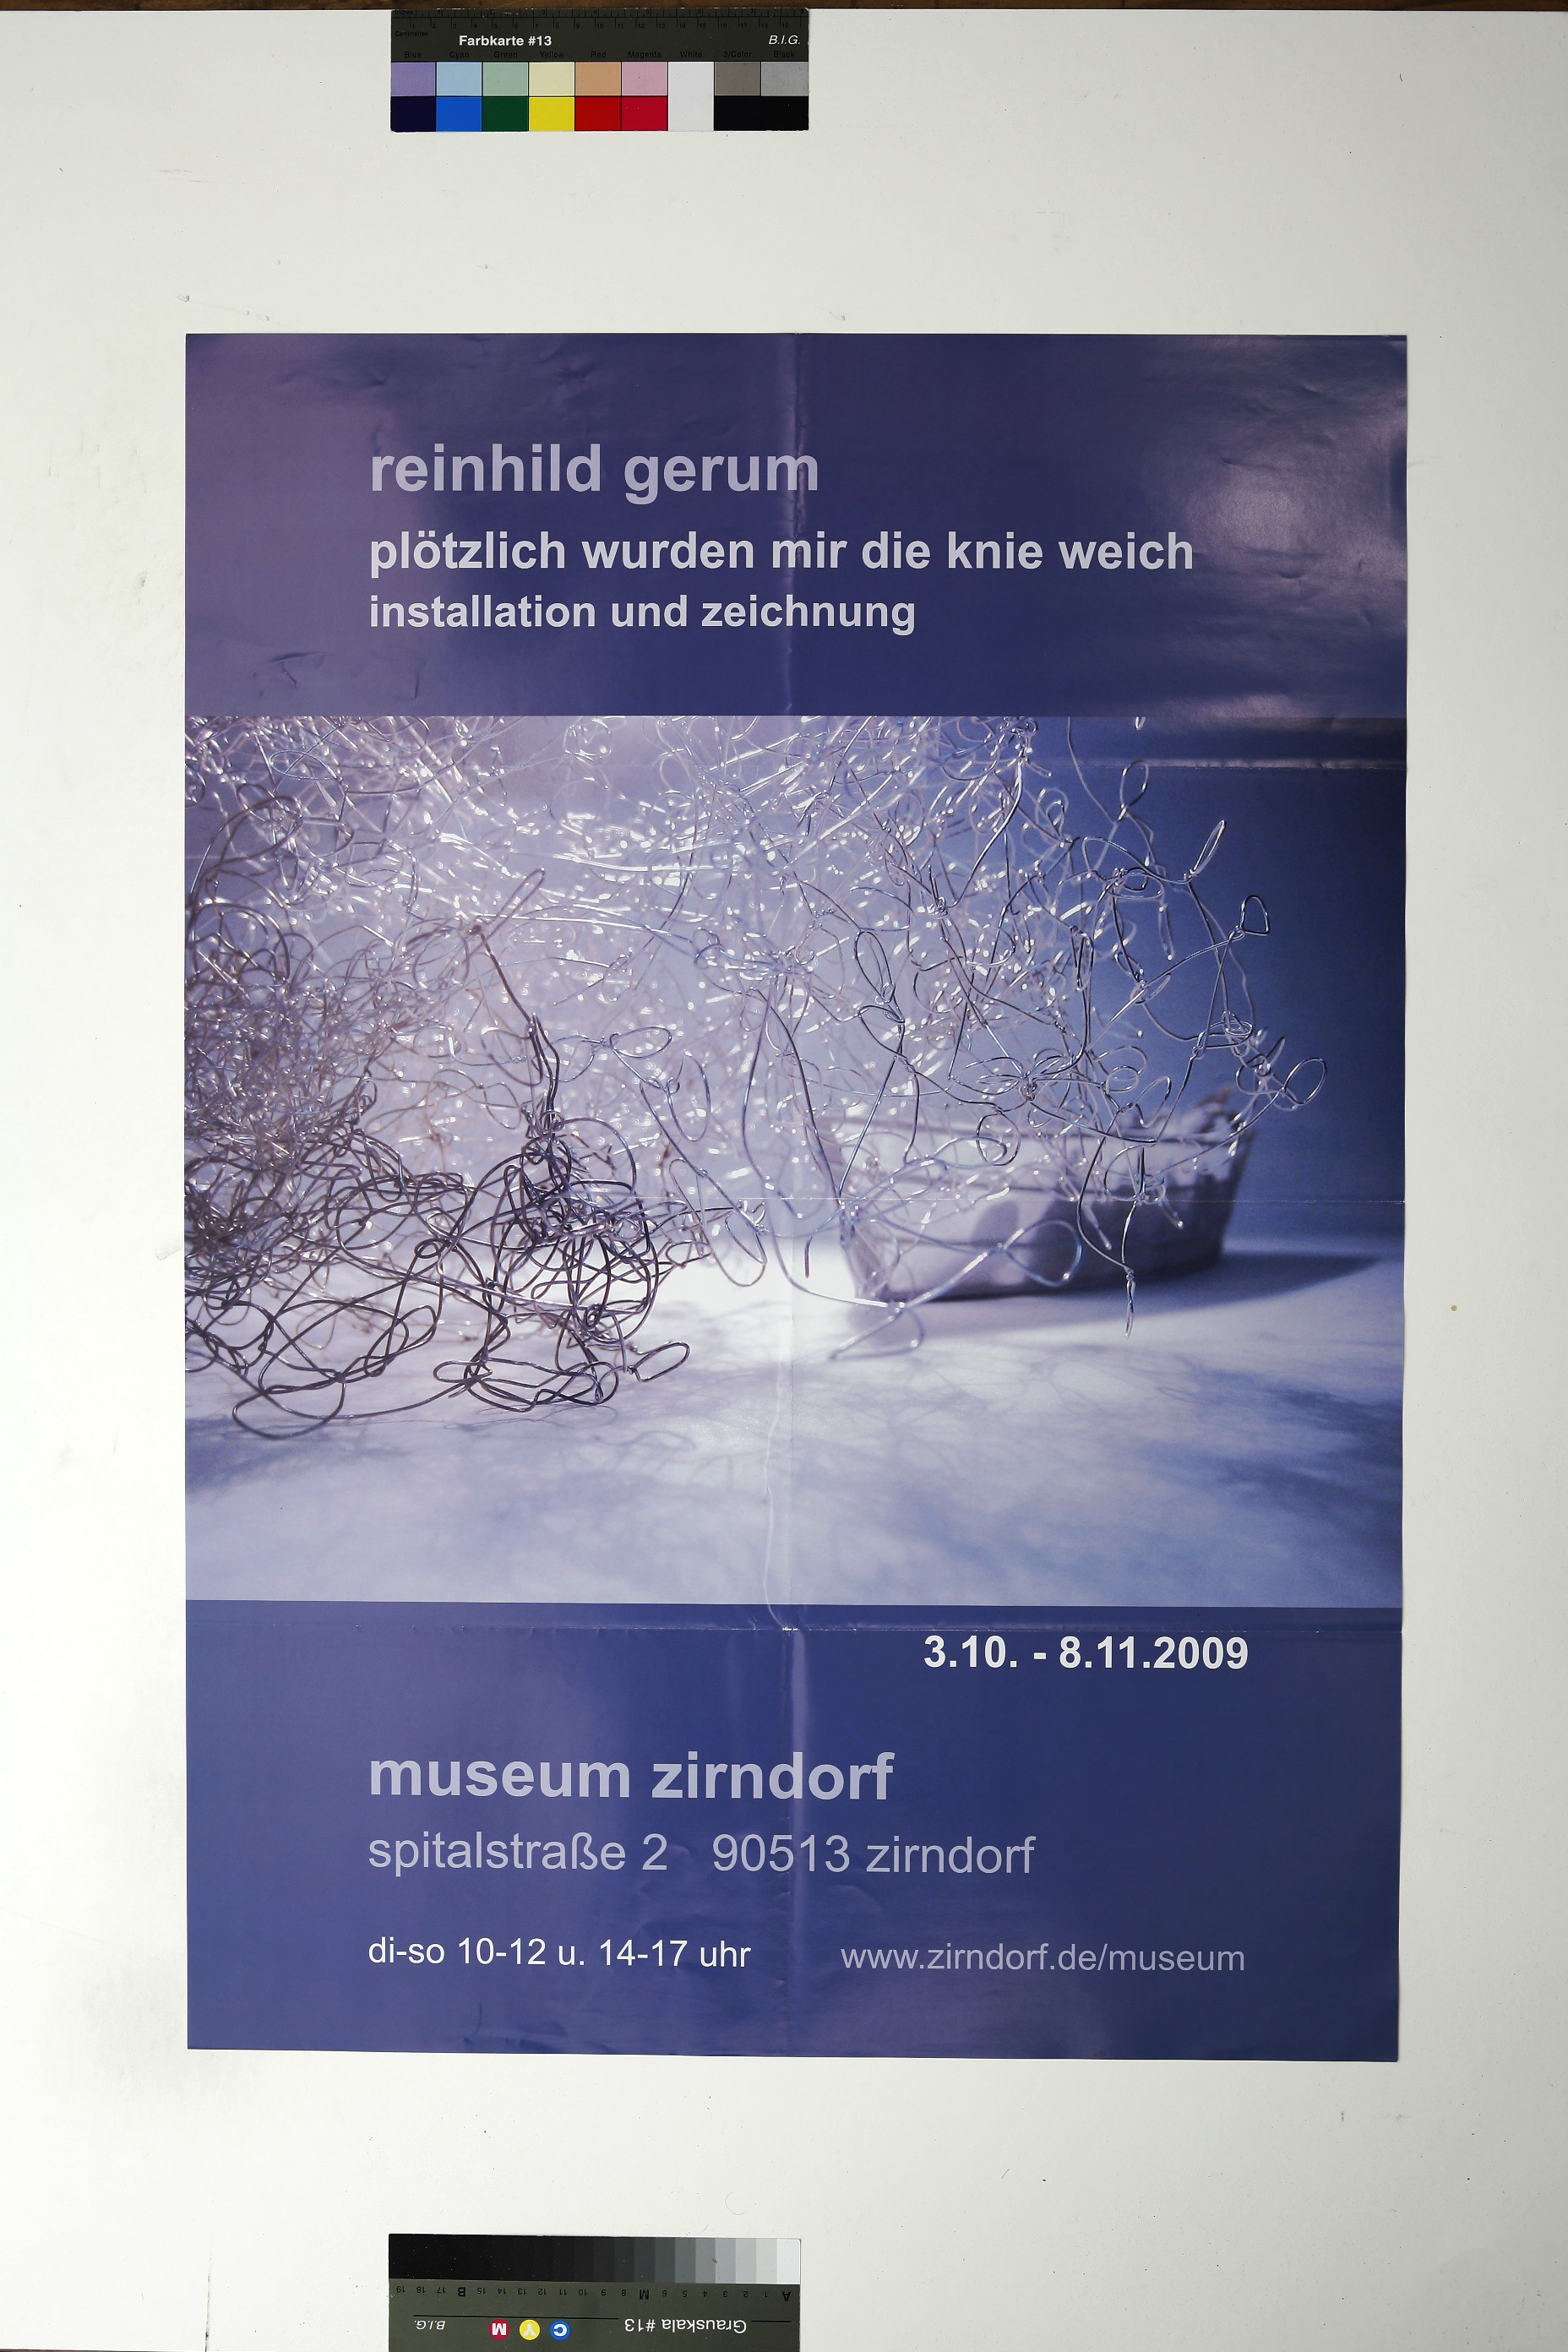
\includegraphics[width=\linewidth]{Abbildung_32_(acht1_128)}
\centering
\caption{Ausstellungsplakat – Reinhild Gerum, Museum Zirndorf, 3.10.2009-08.11.2009 (acht1\_128).}
\end{figure}

\newpage
\begin{figure}[ht]
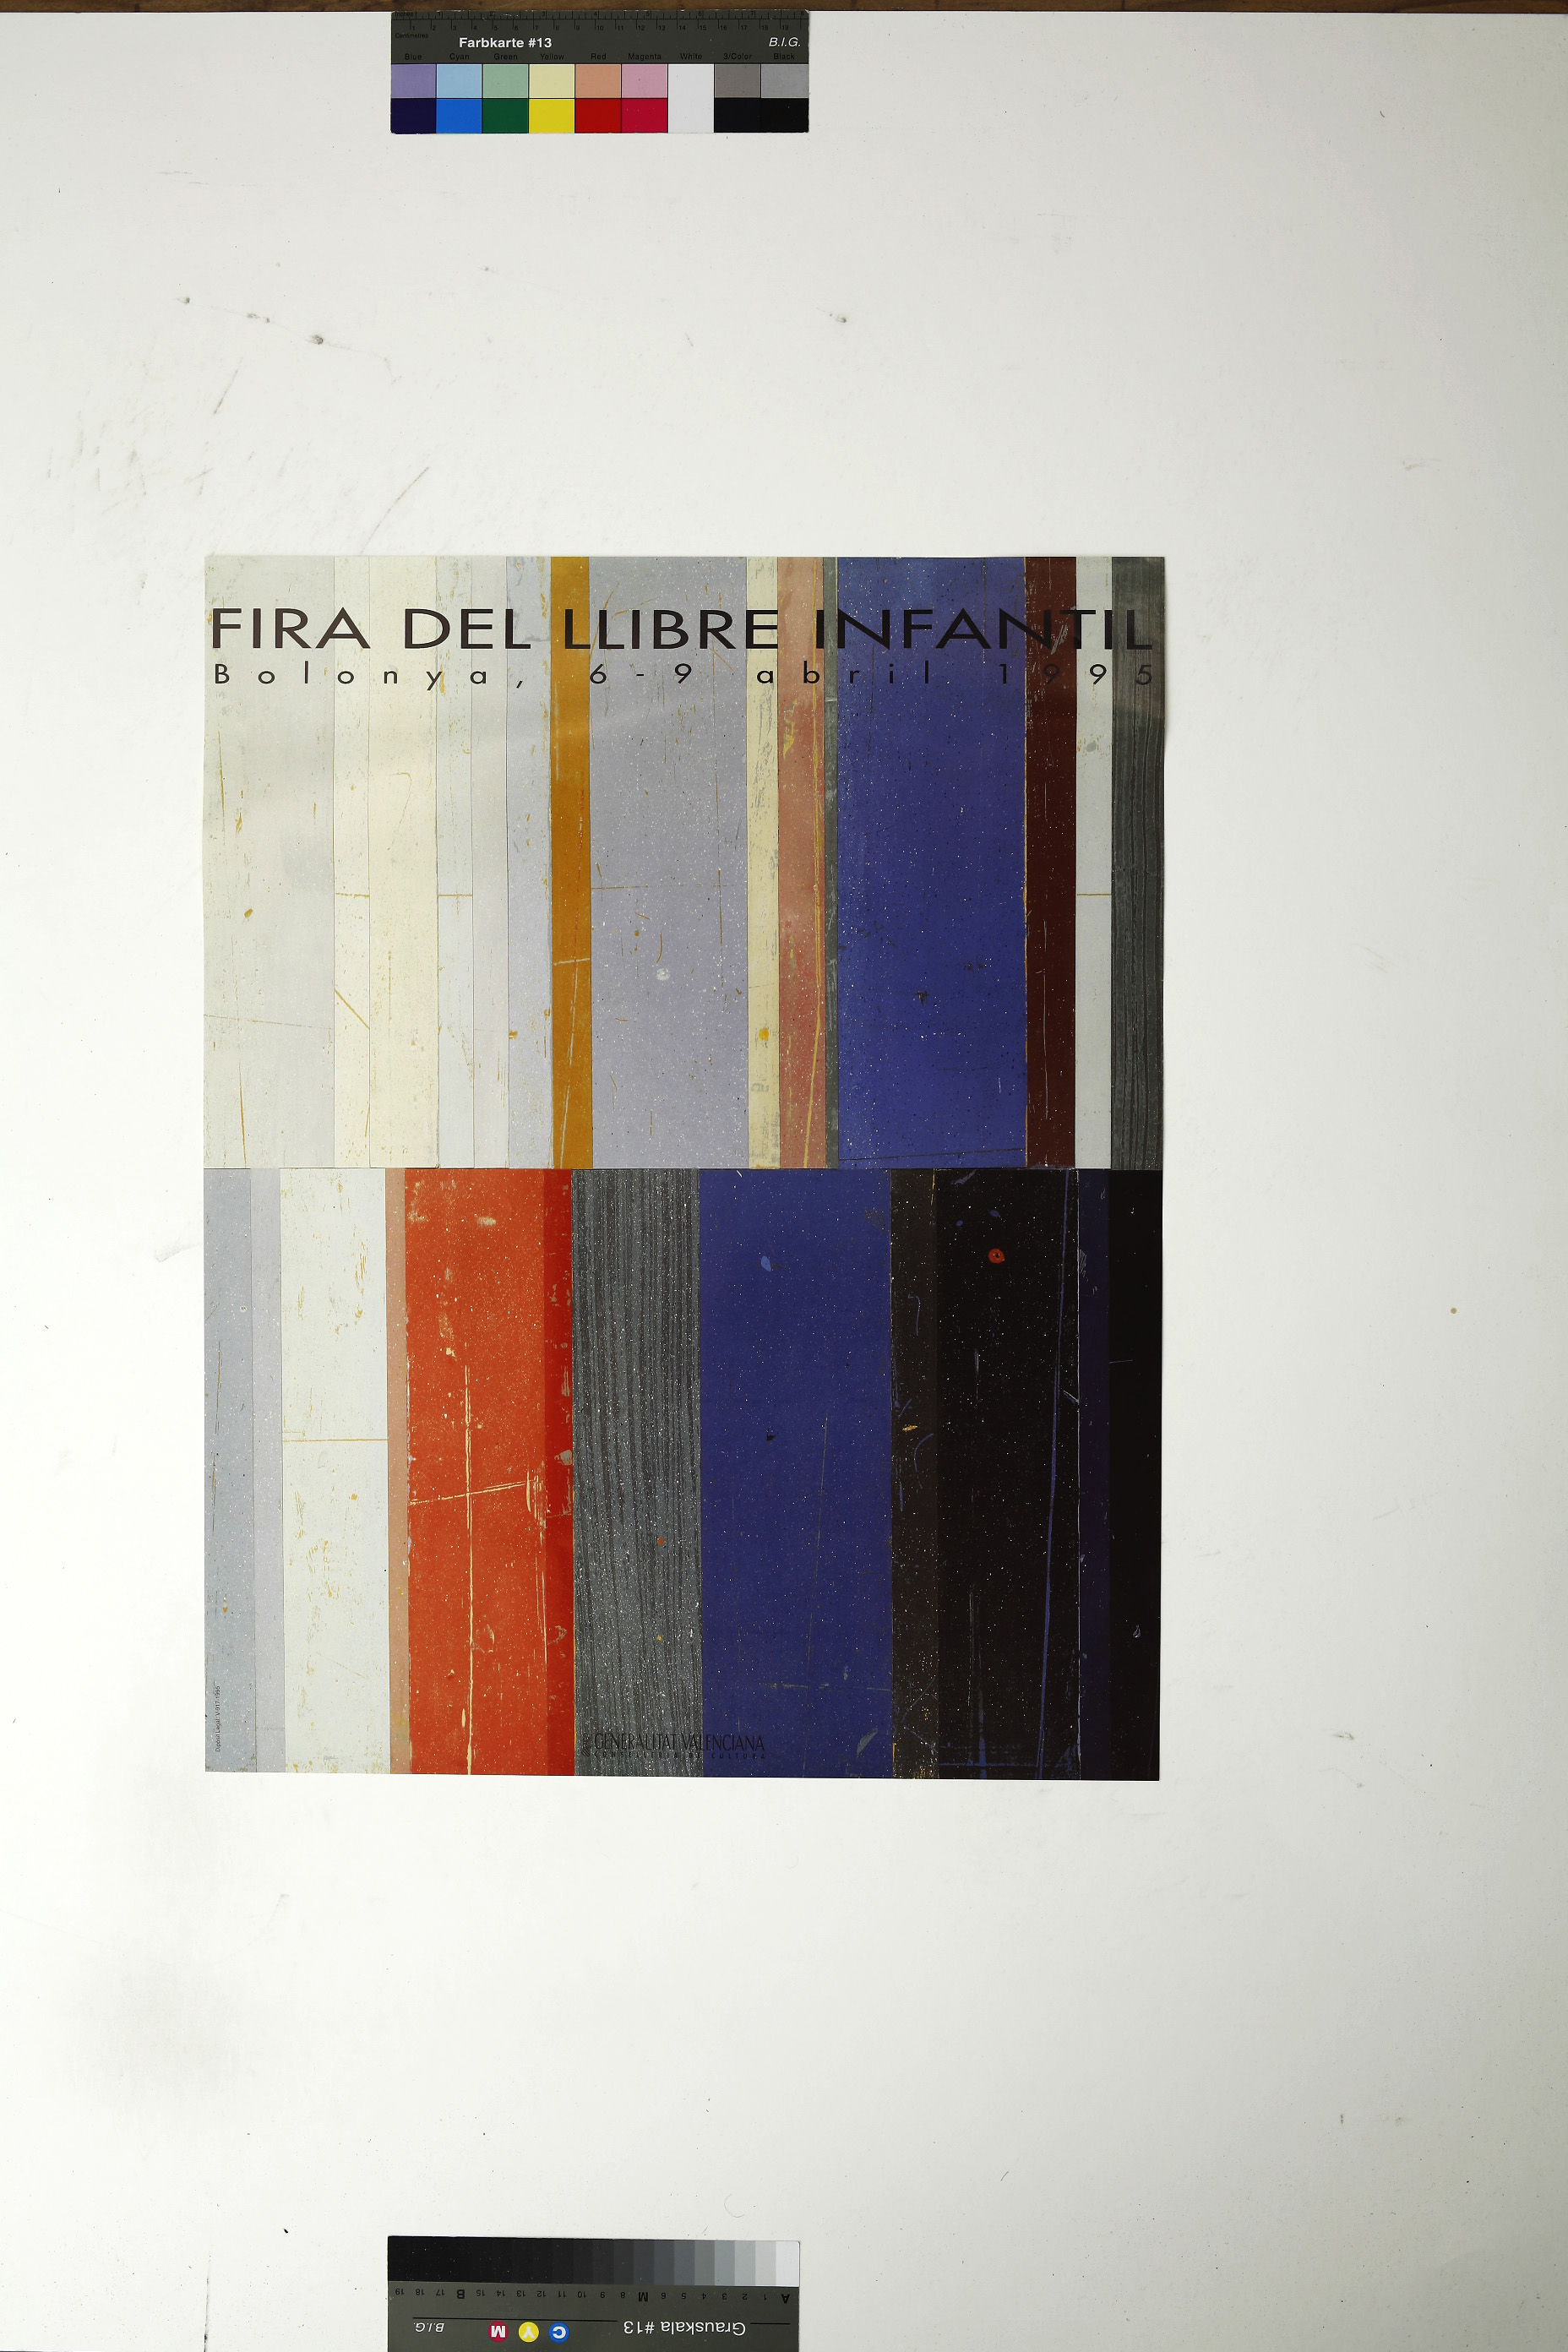
\includegraphics[width=\linewidth]{Abbildung_33_(acht1_021)}
\centering
\caption{Veranstaltungsplakat – Fira del llibre infantil, Bolonya, 06.04.1995-09.04.1995 (acht1\_021).}
\end{figure}

\newpage
\begin{figure}[ht]
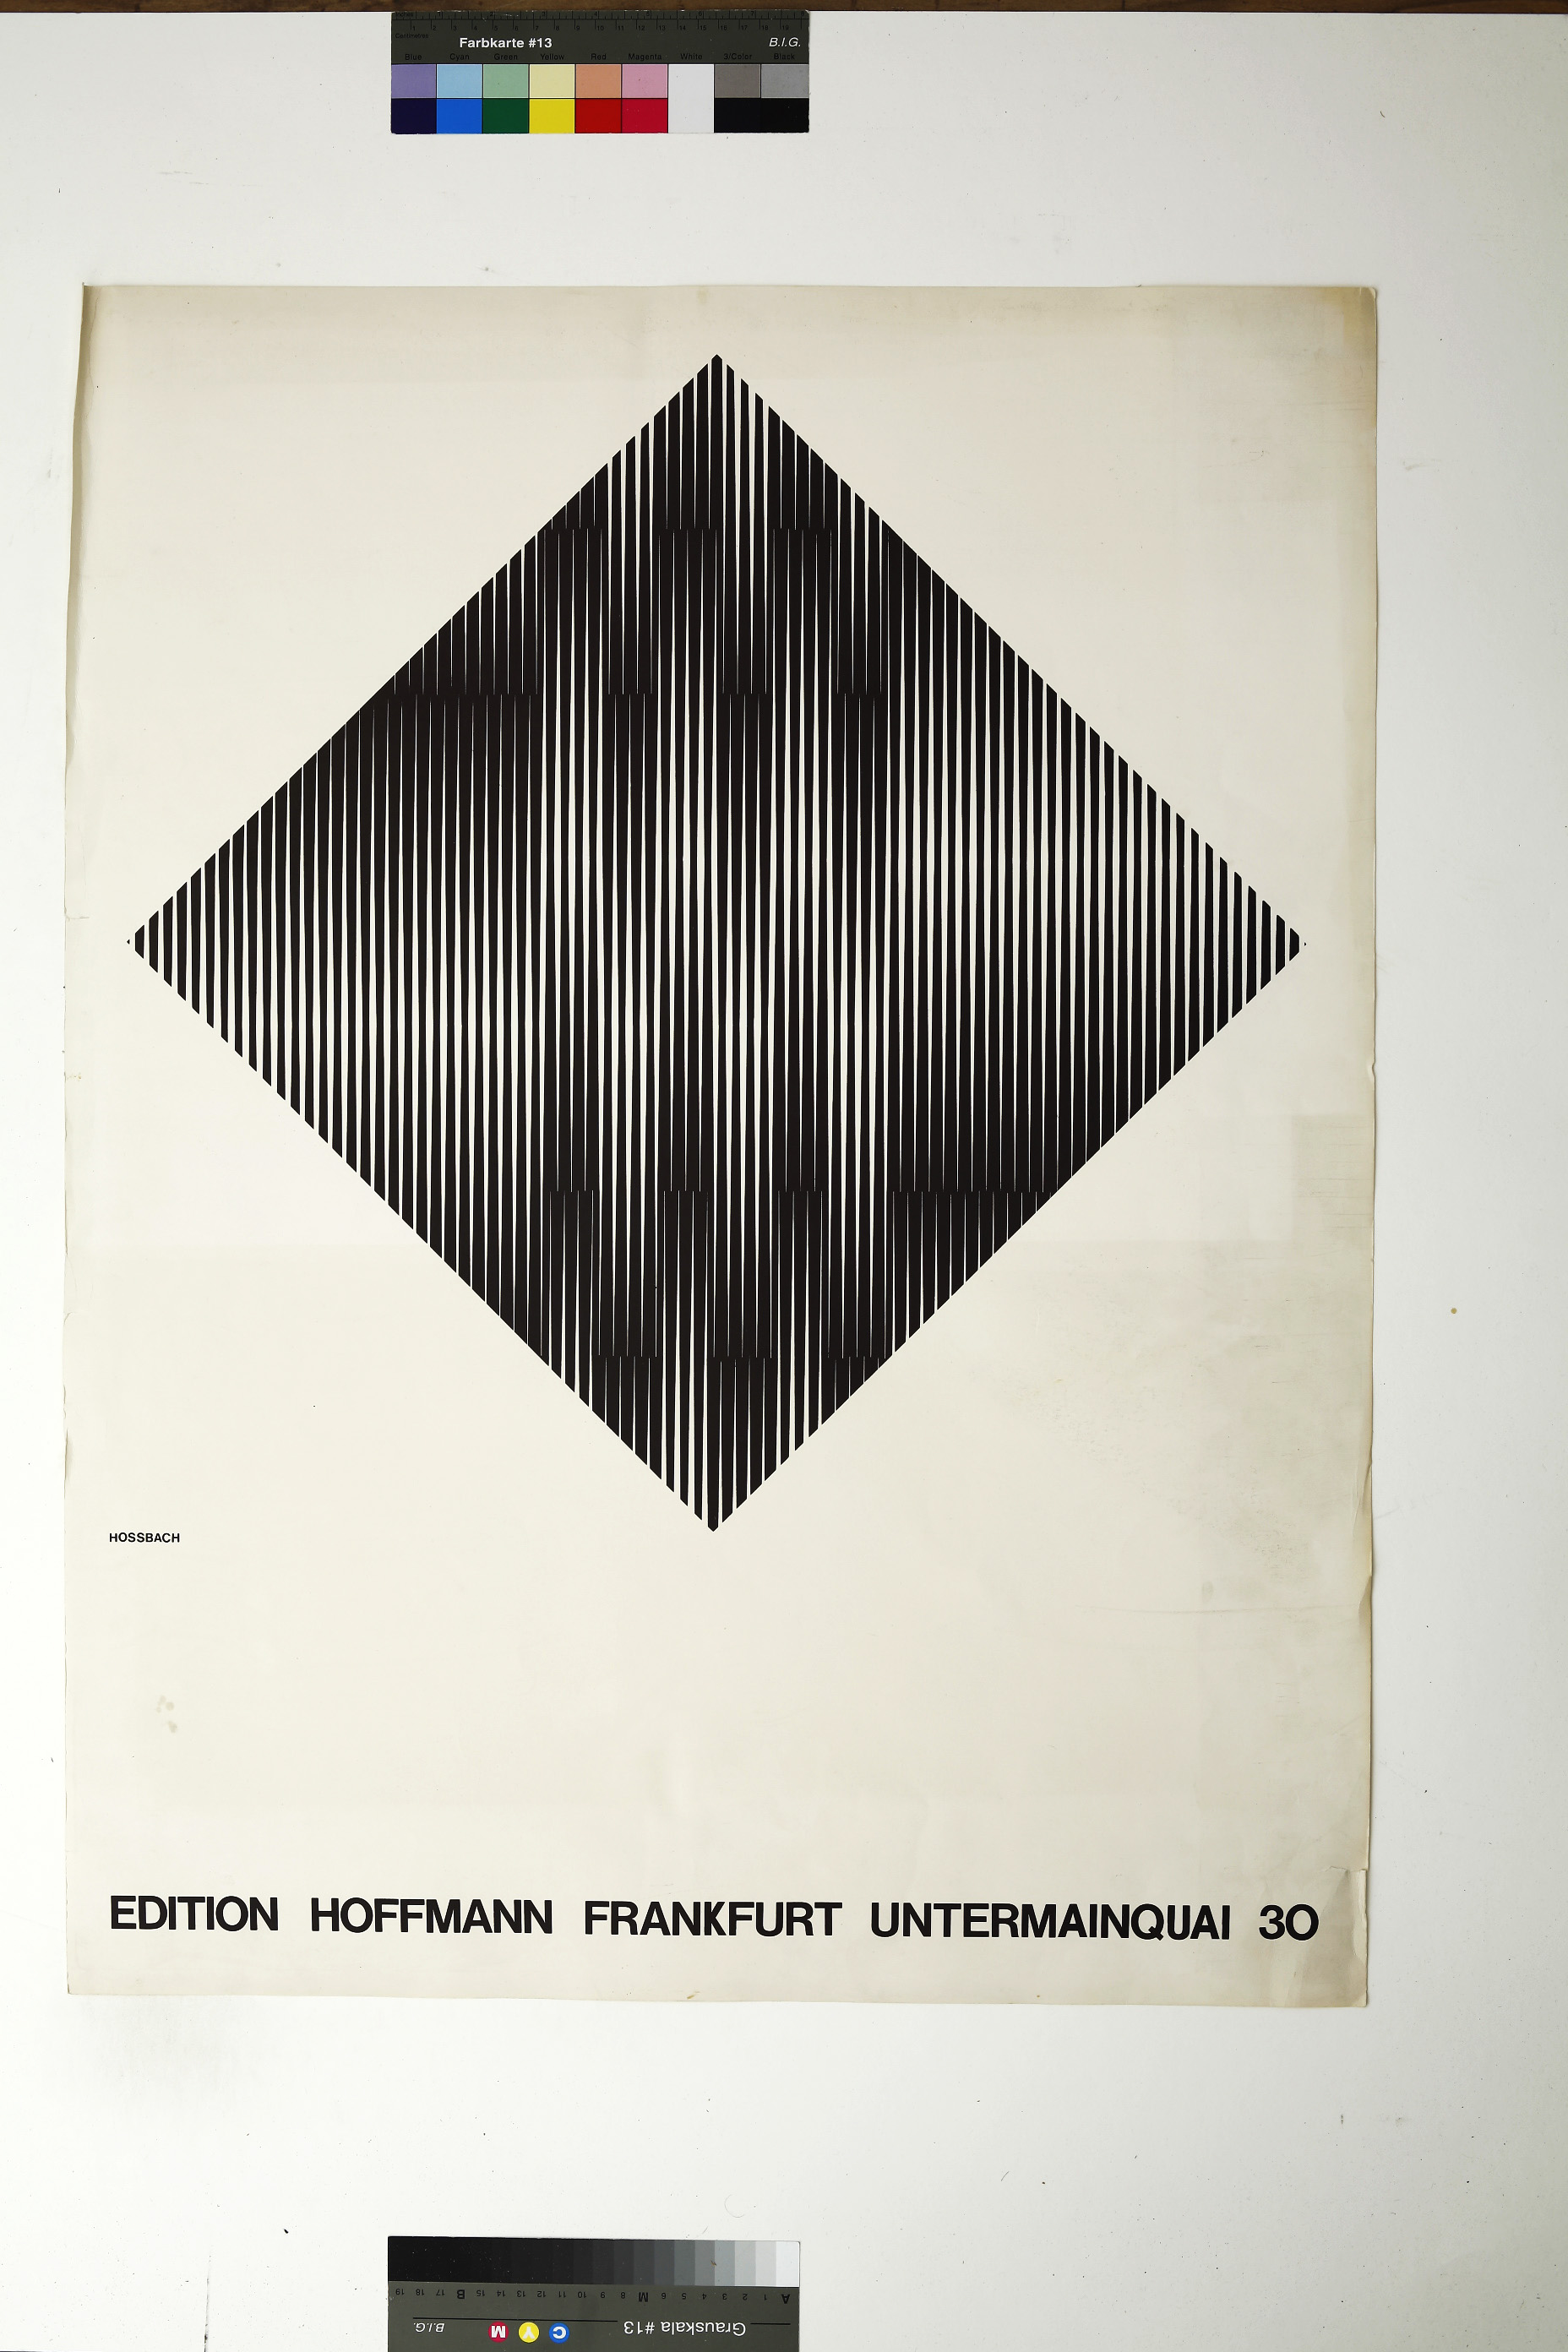
\includegraphics[width=\linewidth]{Abbildung_34_(acht1_058)}
\centering
\caption{Werbeplakat – Edition Hoffmann, ohne Datum (acht1\_058).}
\end{figure}

\newpage
\begin{figure}[ht]
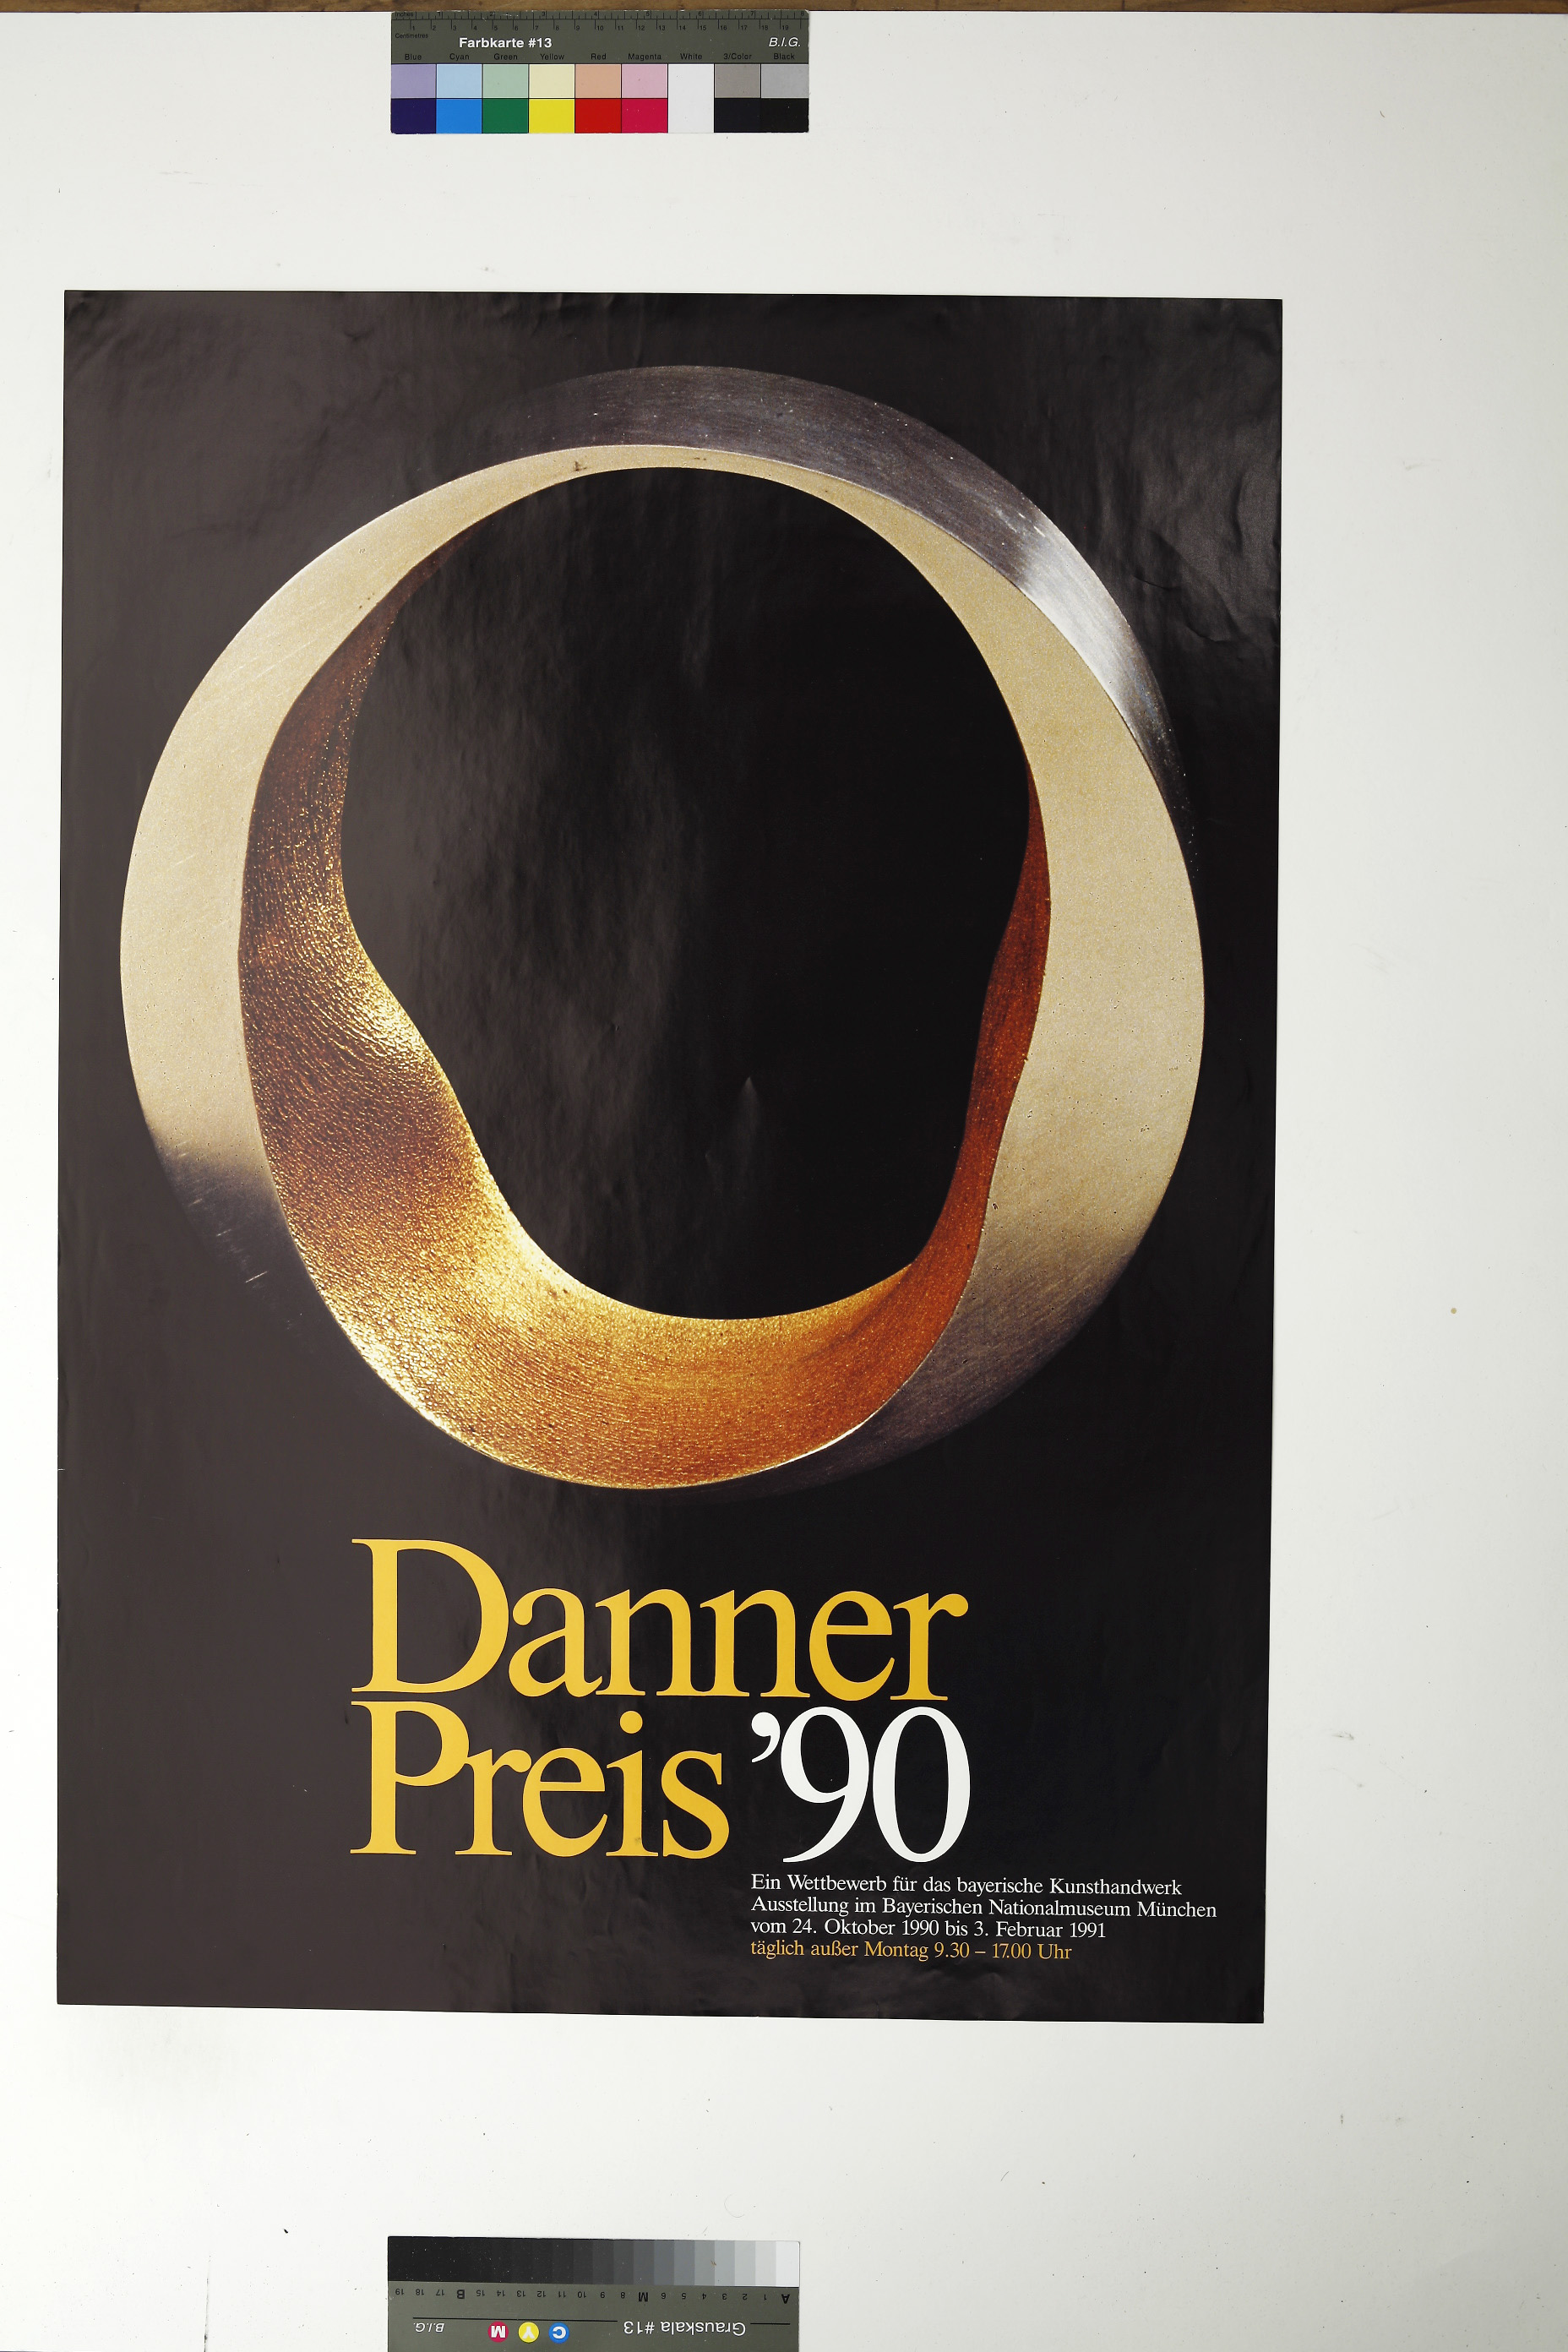
\includegraphics[width=\linewidth]{Abbildung_35_(acht1_043)}
\centering
\caption{Ausstellungsplakat Danner Preis ´90, Bayerisches Nationalmuseum, 24.10.1990-03.02.1991 (acht1\_043).}
\end{figure}

\newpage
\begin{landscape}
\begin{figure}[ht]
	\begin{subfigure}[b]{0.5\linewidth}
	\centering
	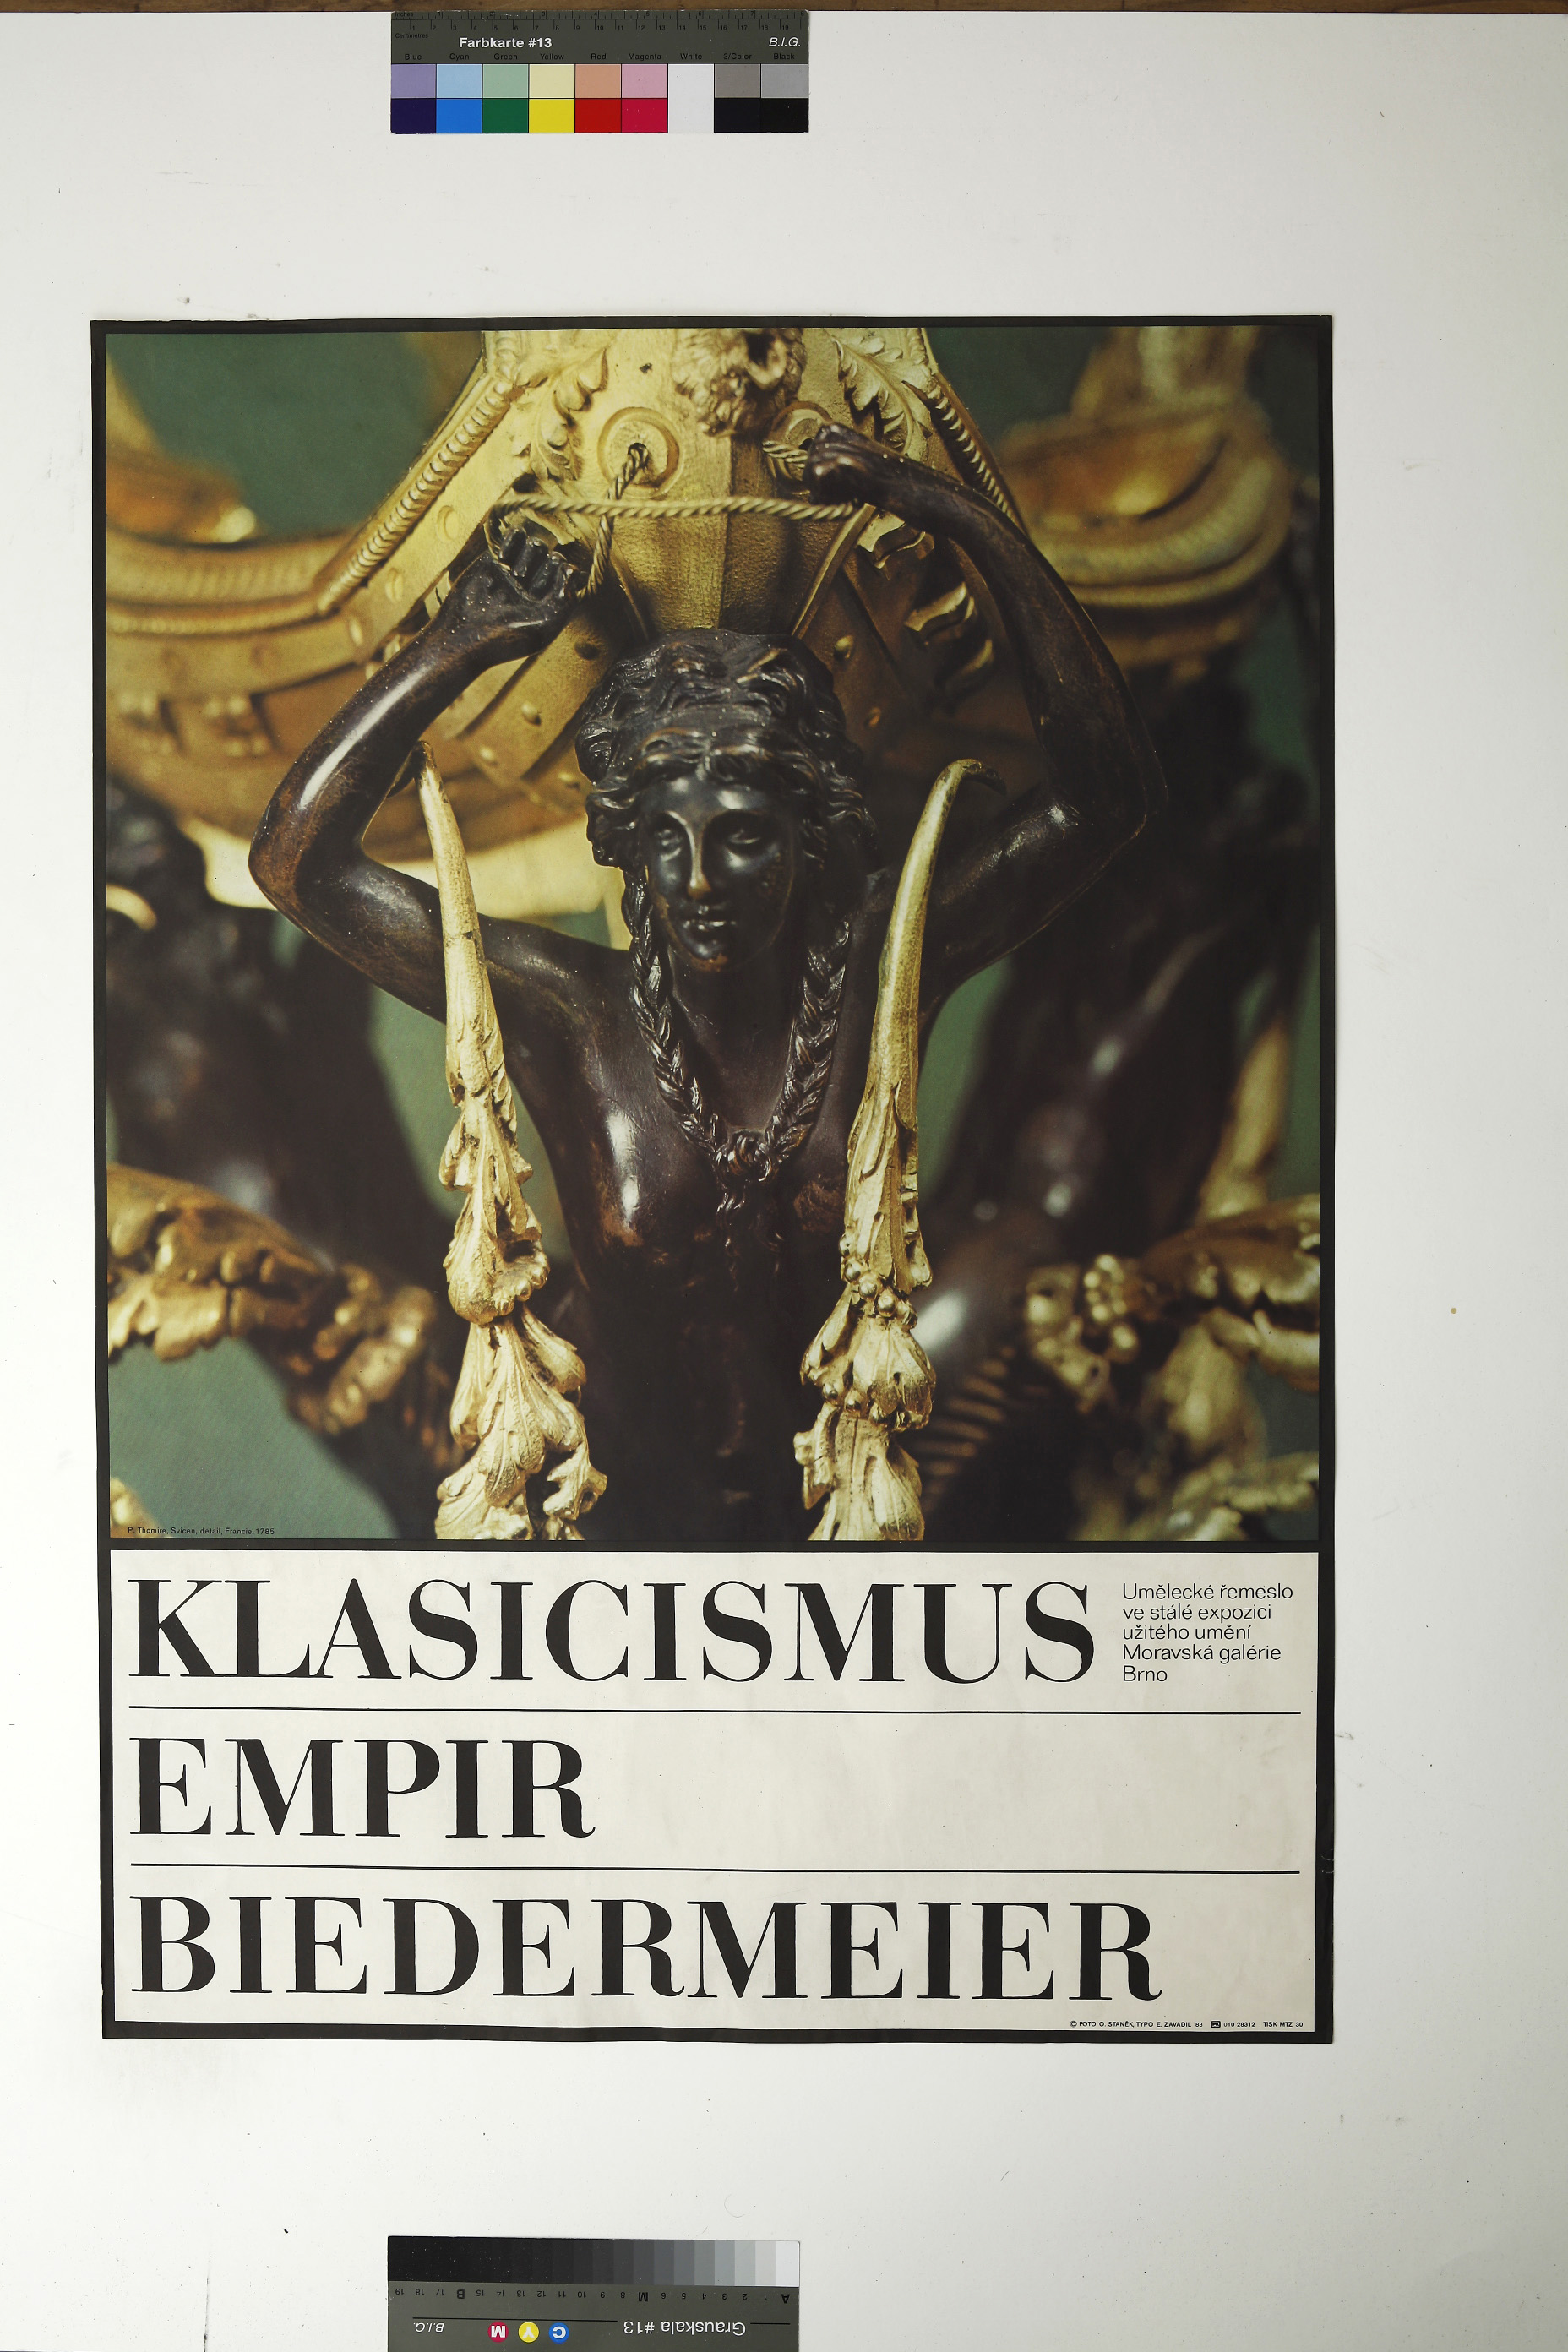
\includegraphics[height=\linewidth]{Abbildung_36_(acht1_029)}
	\end{subfigure}
	\begin{subfigure}[b]{0.5\linewidth}
	\centering
	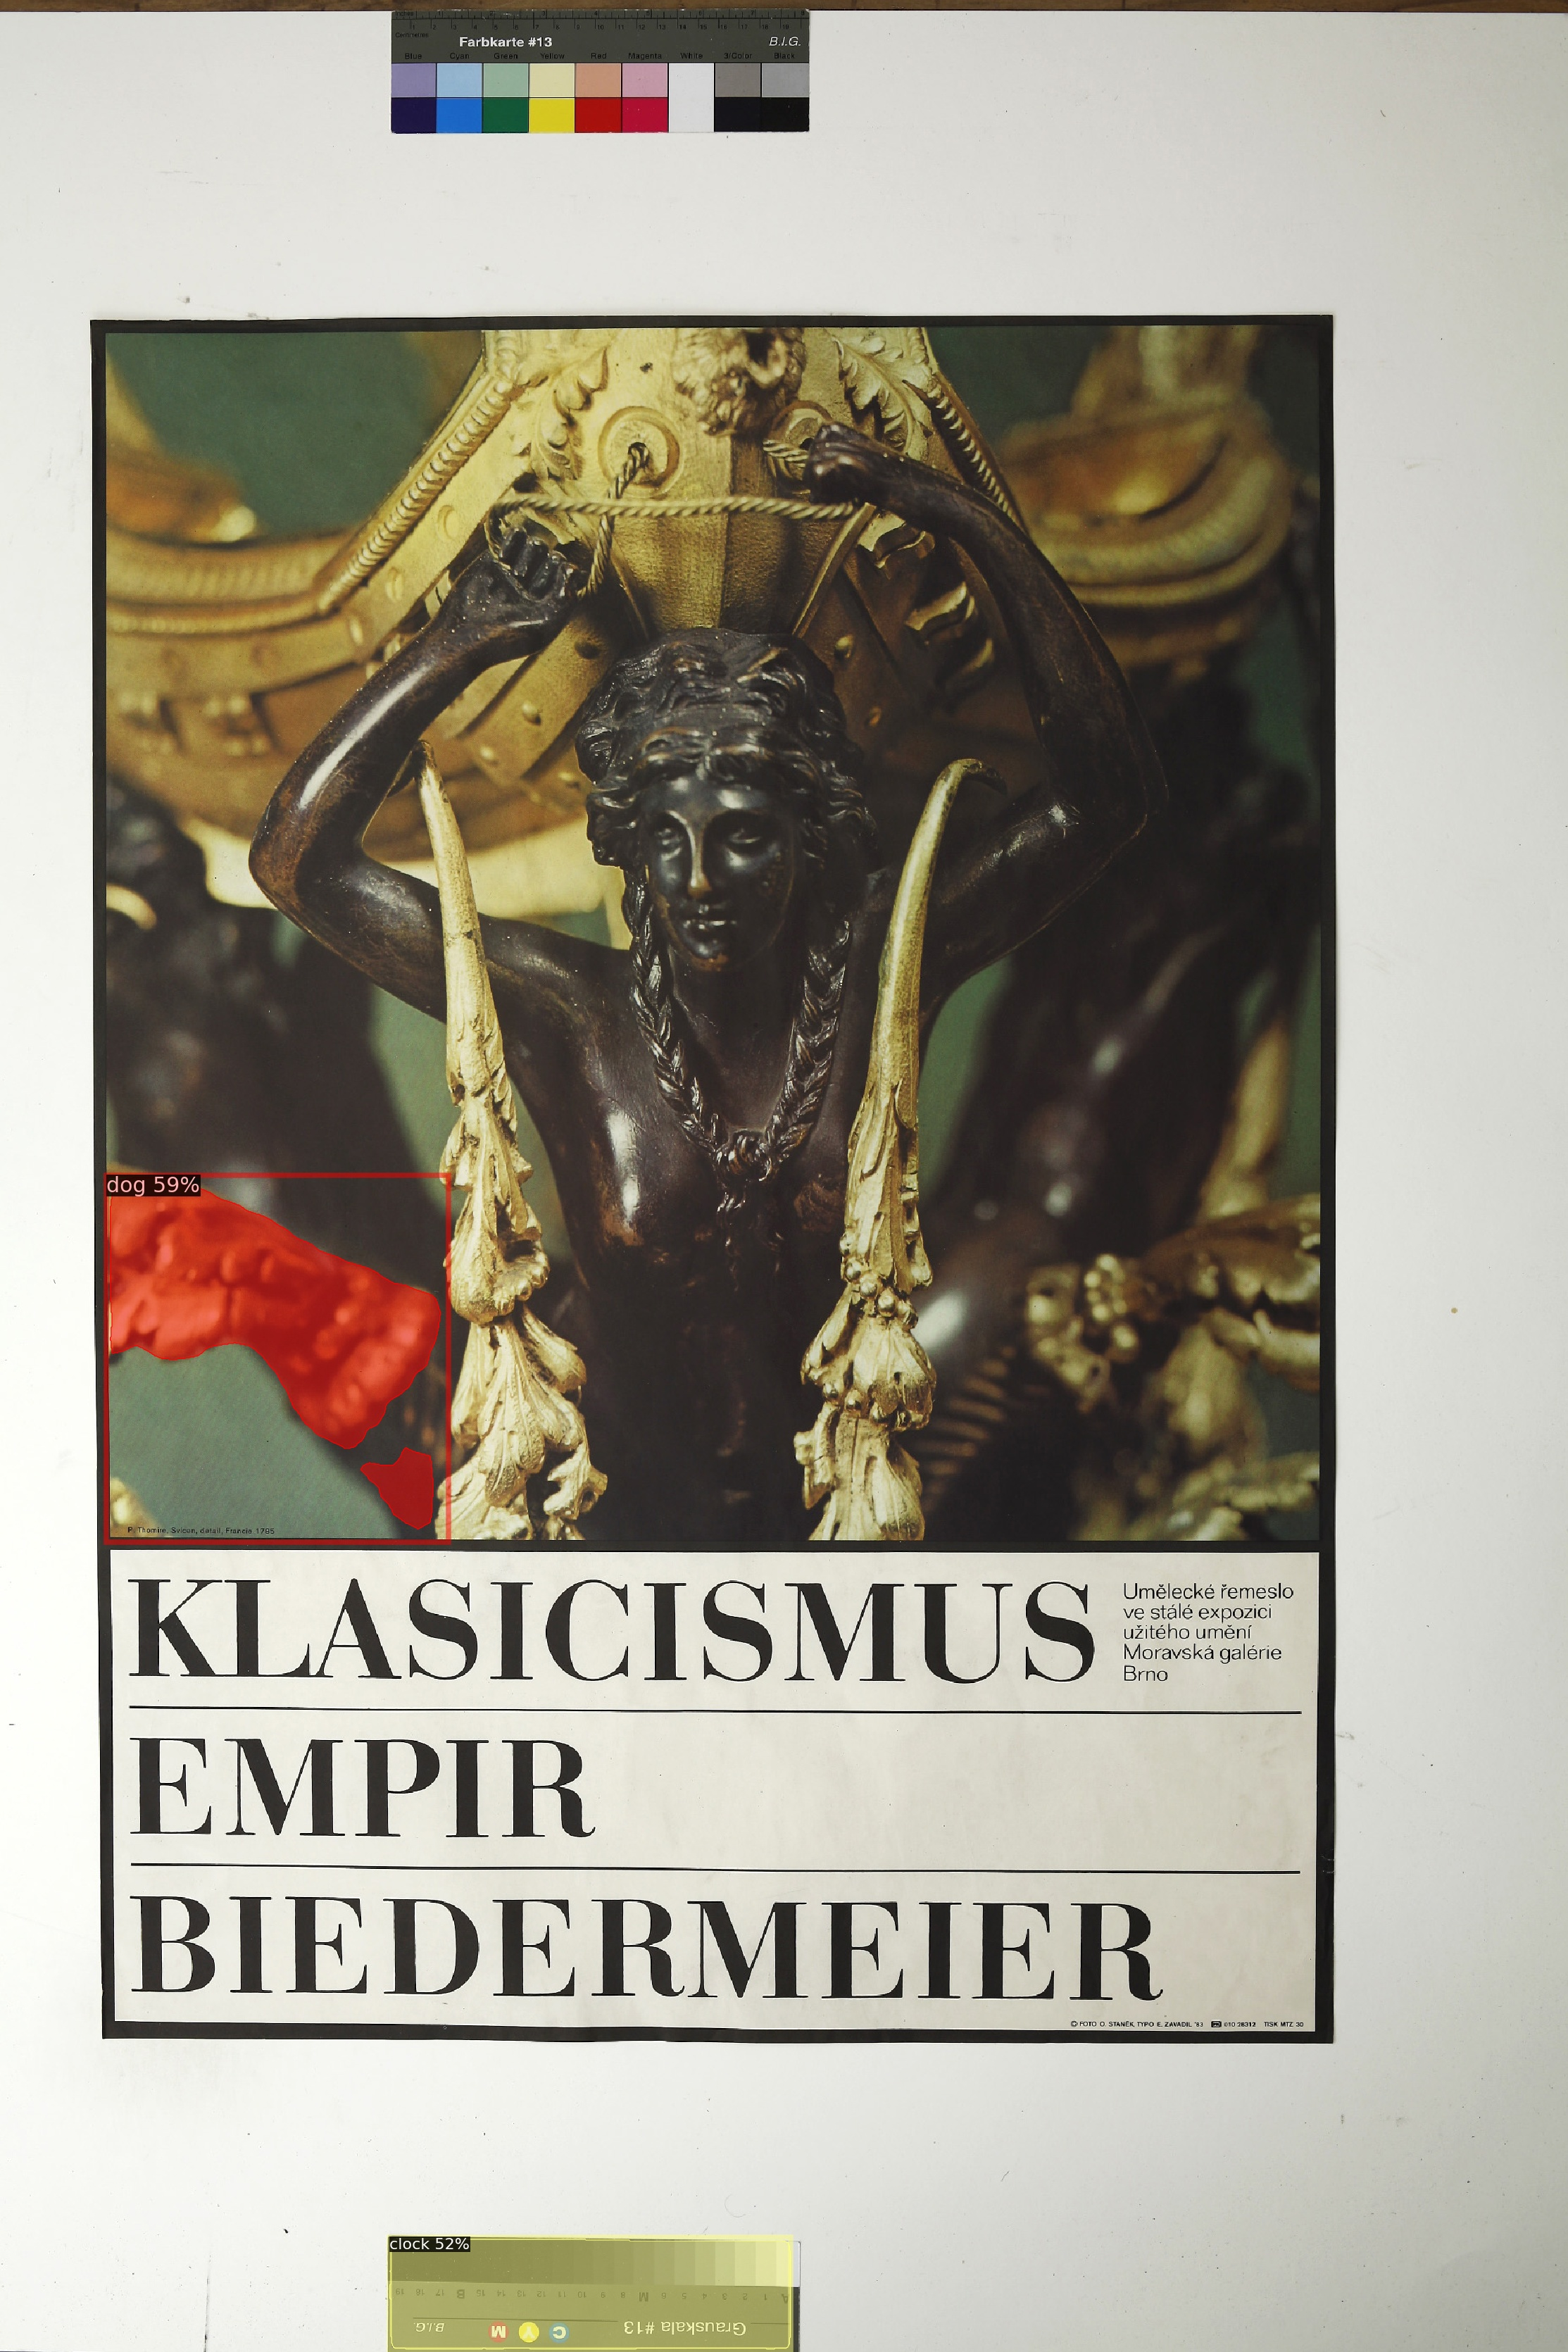
\includegraphics[height=\linewidth]{Abbildung_36_(acht1_029)_with_detections}
	\end{subfigure}
	\caption{Ausstellungsplakat – Klasicismus. Empir. Biedermeier, Moravská galérie Brno, ca. 1983 (acht1\_029); Rechts: Mit Annotationen.}
\end{figure}
\end{landscape}

\newpage
\begin{landscape}
\begin{figure}[ht]
	\begin{subfigure}[b]{0.5\linewidth}
	\centering
	\includegraphics[height=\linewidth]{Abbildung_37_(acht1_038)}
	\end{subfigure}
	\begin{subfigure}[b]{0.5\linewidth}
	\centering
	\includegraphics[height=\linewidth]{Abbildung_37_(acht1_038)_with_detections}
	\end{subfigure}
	\caption{Ausstellungsplakat – Sylva Lacinová, Moravska galerie v Brne, 1983 (acht1\_038); Rechts: Mit Annotationen.}
\end{figure}
\end{landscape}

\newpage
\begin{landscape}
\begin{figure}[ht]
	\begin{subfigure}[b]{0.5\linewidth}
	\centering
	\includegraphics[height=\linewidth]{Abbildung_38_(acht1_108)}
	\end{subfigure}
	\begin{subfigure}[b]{0.5\linewidth}
	\centering
	\includegraphics[height=\linewidth]{Abbildung_38_(acht1_108)_with_detections}
	\end{subfigure}
	\caption{Ausstellungsplakat – Henry Moore. Shelter Drawings, Rupertinum, 23.07.1994-23.10.1994 (acht1\_108); Rechts: Mit Annotationen.}
\end{figure}
\end{landscape}

\newpage
\begin{figure}[ht]
\includegraphics[width=\linewidth]{Abbildung_39_(acht1_034)}
\centering
\caption{Ausstellungsplakat – Cèské umèní 20. století, Moravská galerie Brno, ohne Datum (acht1\_034).}
\end{figure}

\newpage
\begin{landscape}
\begin{figure}[ht]
	\begin{subfigure}[b]{0.5\linewidth}
	\centering
	\includegraphics[height=\linewidth]{Abbildung_40_(acht2_147)}
	\end{subfigure}
	\begin{subfigure}[b]{0.5\linewidth}
	\centering
	\includegraphics[height=\linewidth]{Abbildung_40_(acht2_147)_with_detections}
	\end{subfigure}
	\caption{Werbeplakat – Wenn Frau will, steht alles still. Landesweiter Frauenstreik, 14.06.1991 (acht2\_147); Rechts: Mit Annotationen.}
\end{figure}
\end{landscape}

\newpage
\begin{landscape}
\begin{figure}[ht]
	\begin{subfigure}[b]{0.5\linewidth}
	\centering
	\includegraphics[height=\linewidth]{Abbildung_41_(acht3_006)}
	\end{subfigure}
	\begin{subfigure}[b]{0.5\linewidth}
	\centering
	\includegraphics[height=\linewidth]{Abbildung_41_(acht3_006)_with_detections}
	\end{subfigure}
	\caption{Werbeplakat – Graswurzelrevolution. Monatszeitung für eine gewaltfreie, herrschaftslose Gesellschaft, ohne Datum (acht3\_006); Rechts: Mit Annotationen.}
\end{figure}
\end{landscape}

\newpage
\begin{figure}[ht]
\includegraphics[width=\linewidth]{Abbildung_42_(acht3_433)}
\centering
\caption{Werbeplakat – Jede Großstadt hat das Verbrechen, das sie verdient. Berlin Crime, edition monade Verlag, ohne Datum (acht3\_433).}
\end{figure}

\newpage
\begin{figure}[ht]
\includegraphics[width=\linewidth]{Abbildung_43_(acht1_053)}
\centering
\caption{Veranstaltungsplakat – Reveillon de Printemps de la création et de la culture, 13.06.1992 (acht1\_053).}
\end{figure}

\newpage
\begin{landscape}
\begin{figure}[ht]
	\begin{subfigure}[b]{0.5\linewidth}
	\centering
	\includegraphics[height=\linewidth]{Abbildung_44_(acht1_124)}
	\end{subfigure}
	\begin{subfigure}[b]{0.5\linewidth}
	\centering
	\includegraphics[height=\linewidth]{Abbildung_44_(acht1_124)_with_detections}
	\end{subfigure}
	\caption{Ausstellungsplakat - Fokus Franken. Triennale Schweinfurt für Zeitgenössische Kunst, Kunsthalle Schweinfurt, 13.11.2009-14.02.2010 (acht1\_124); Rechts: Mit Annotationen.}
\end{figure}
\end{landscape}

\newpage
\begin{figure}[ht]
\includegraphics[width=\linewidth]{Abbildung_45_(acht1_094)}
\centering
\caption{Ausstellungsplakat - Joe Allen. Spuren und Fährten. Malerei 1996-2006, Museum Schloss Moyland, 02.06.2006-15.10.2006 (acht1\_094).}
\end{figure}

\newpage
\begin{landscape}
\begin{figure}[ht]
\includegraphics[height=0.85\linewidth, angle=90]{Abbildung_46_(acht2_003)}
\centering
\caption{Dekoratives Plakat – Mimmo Rotella: Gutenberg 2000, 2000 (acht2\_003).}
\end{figure}
\end{landscape}

\newpage
\begin{figure}[ht]
\includegraphics[width=\linewidth]{Abbildung_47_(acht2_163)}
\centering
\caption{Ausstellungsplakat - frauenobjektiv. Fotografinnen 1940 bis 1950, Haus der Geschichte der Bundesrepublik Deutschland, 18.05.2001 - 29.07.2001 (acht2\_163).}
\end{figure}

\newpage
\begin{figure}[ht]
\includegraphics[width=\linewidth]{Abbildung_48_(acht2_148)}
\centering
\caption{Veranstaltungsplakat – Paroles de femmes, Fédération des Oeuvres Laiques, ohne Datum (acht2\_148).}
\end{figure}

\newpage
\begin{figure}[ht]
\includegraphics[width=\linewidth]{Abbildung_49_(zehn1_085)}
\centering
\caption{Ausstellungsplakat – Udo Lindenberg. Wo ich meinen Hut hinhäng..., Museum Schloss Moyland, 08.07.2000-20.08.2000 (zehn1\_085).}
\end{figure}

\newpage
\begin{landscape}
\begin{figure}[ht]
	\begin{subfigure}[b]{0.5\linewidth}
	\centering
	\includegraphics[height=\linewidth]{Abbildung_50_(acht1_033)}
	\end{subfigure}
	\begin{subfigure}[b]{0.5\linewidth}
	\centering
	\includegraphics[height=\linewidth]{Abbildung_50_(acht1_033)_with_detections}
	\end{subfigure}
	\caption{Ausstellungsplakat – Ceské moderní malírství (II), Dum Umení Mesta Brna, 17.05.1983-03.07.1983 (acht1\_033); Rechts: Mit Annotationen.}
\end{figure}
\end{landscape}

\newpage
\begin{figure}[ht]
\includegraphics[width=\linewidth]{Abbildung_51_(acht2_033)}
\centering
\caption{Veranstaltungsplakat – Expobat[..]. Bateaux neufs habitables a flot, 07./15.09.1974 (acht2\_033).}
\end{figure}

\newpage
\begin{figure}[ht]
	\begin{subfigure}[b]{\linewidth}
	\centering
	\includegraphics[height=\linewidth, angle=90]{Abbildung_52_(achtzehn2_025)}
	\end{subfigure}
	\begin{subfigure}[b]{\linewidth}
	\centering
	\includegraphics[height=\linewidth, angle=90]{Abbildung_52_(achtzehn2_025)_with_detections}
	\end{subfigure}
	\caption{Ausstellungsplakat – Günter Eich 1907-19[…], Deutsches Literaturarchiv, 09.04.-28.[…] (achtzehn2\_025); Unten: Mit Annotationen.}
\end{figure}

\newpage
\begin{figure}[ht]
\includegraphics[width=\linewidth]{Abbildung_53_(elf4_300)}
\centering
\caption{Veranstaltungsplakat – Fire Red Pon Babylon. Turbulence. Chezidek. Lutan Fyah, Elysée Montmartre, 14.04. (elf4\_300).}
\end{figure}

\newpage
\begin{landscape}
\begin{figure}[ht]
	\centering
	\includegraphics[height=0.49\linewidth]{Abbildung_54a_(acht2_074)}
	\centering
	\includegraphics[height=0.49\linewidth]{Abbildung_54b_(acht2_074)}
	\centering
	\includegraphics[height=0.49\linewidth]{Abbildung_54c_(acht2_074)}
	\caption{Veranstaltungsplakat – Herr Senator Carl-Heinz Evers. Die Entwicklung des Berliner Erziehungswesens im europäischen Vergleich, Amerika-Gedenkbibliothek am Halleschen Tor, 5.11.1963 (acht2\_074); Mitte: Detection mit einem adaptiven Threshold; Rechts: Detection mit globalem Threshold.}
\end{figure}
\end{landscape}

\newpage
\begin{figure}[ht]
\includegraphics[width=\linewidth]{Labelme_Screenshot}
\centering
\caption{Screenshot eines annotierten Plakats in der Software \textit{Labelme}.}
\end{figure}

\newpage
\begin{figure}[ht]
\includegraphics[width=\linewidth]{Ellbow_Method}
\centering
\caption{Ermittlung der Optimalen Anzahl an Clustern durch die \textit{Ellbow Method}.}
\end{figure}

\newpage
\begin{landscape}
\begin{figure}[ht]
	\begin{subfigure}[b]{0.5\linewidth}
	\centering
	\includegraphics[height=\linewidth]{4_clusters_untrained}
	\end{subfigure}
	\begin{subfigure}[b]{0.5\linewidth}
	\centering
	\includegraphics[height=\linewidth]{8_clusters_untrained}
	\end{subfigure}
	\caption{Verteilung der Plakatkategorien zwischen den einzelnen Clustern mit einem untrainierten Modell}
\end{figure}
\end{landscape}

\newpage
\begin{figure}[ht]
\includegraphics[width=\linewidth]{image_cluster_untrained}
\centering
\caption{Darstellung des geclusterten Tensorflow Datensatz durch ein untrainiertes Modell.}
\end{figure}

\newpage
\begin{figure}[ht]
\includegraphics[width=\linewidth]{first_training}
\centering
\caption{Entwicklung von Genauigkeit und \textit{Loss} während dem ersten Training.}
\end{figure}

\newpage
\begin{figure}[ht]
\includegraphics[width=\linewidth]{second_training}
\centering
\caption{Entwicklung von Genauigkeit und \textit{Loss} während dem zweiten Training.}
\end{figure}


\newpage
\section{Anlagen}
\subsection{Fragebogen: Fragen bezüglich der Digitalisierung}
\begin{enumerate}
\item Ist die Plakatsammlung digital erschlossen, beziehungsweise ist eine Erschließung in Planung?
\item Ist die komplette Sammlung digitalisiert worden?
\begin{enumerate}
\item Wenn nein: Wie groß ist der erschlossene Teil und ist eine weitere Erschließung geplant?
\end{enumerate}
\item Gibt es eine Datenbankstruktur, in der die Sammlung abgebildet wird?
\item In welchem Format liegt die Sammlung vor?
\item Gibt es Metadaten für die konkreten Werke?
\item Sind diese Daten normiert?
\item Konnte man auf eine Datengrundlage aus dem Archiv zurückgreifen?
\item Gibt es Pläne, die Plakatsammlung in eine gewisse Richtung weiterzuentwickeln?
\item Wird die Digitalisierung Hausintern bewältigt oder bestehen Kooperationen?
\begin{enumerate}
\item Gab es Probleme bei Versuchen der Kooperation?
\end{enumerate}
\item Gibt es aktuelle Projekte und Forschungsarbeiten, die sich mit der Plakatsammlung beschäftigen?
\item Ist die Sammlung digital einer Öffentlichkeit zugänglich oder ist derartiges geplant?
\begin{enumerate}
\item Wenn ja: Wer ist die Zielgruppe und wie wird in der Präsentation der Sammlung auf diese Gruppe Bezug genommen?
\end{enumerate}
\item Wird die Sammlung nur auf der Museumswebsite präsentiert?
\begin{enumerate}
\item Wenn ja: Ist es geplant die Sammlung auch durch andere Quellen verfügbar zu machen? (Prometheus)
\end{enumerate}
\item Ist Urheberrecht für Sie ein Problem?
\item Ist Digitalisierung ein erstrebenswertes Ziel?
\item Ist Digitalisierung um jeden Preis richtig?
\begin{enumerate}
\item Gibt es in dem Sinn rote Linien?
\end{enumerate}
\item Braucht ein Museum eine digitale Sammlung, um zukunftsfähig zu sein?
\item Wie bewerten Sie den Stand der Digitalisierung in den deutschen Museen und in ihrem eigenen?
\item Was trifft eher zu: „Die Digitalisierung ist ein Prozess, der durch eine Verteilung in mehreren Häusern mehr Innovativkraft freisetzen kann.“ oder „Die Digitalisierung ist am besten zentral und im gesamten Bundesgebiet von einer Institution zu steuern, um eine Einheitlichkeit zu gewährleisten.
\end{enumerate}

\newpage
\section{Literaturverzeichnis}
\subsection{Links}

\begin{itemize}
\item A Dictionary of Computer Science, Machine Learning: \href{https://www.oxfordreference.com/view/10.1093/acref/9780199688975.001.0001/acref-9780199688975-e-3056?rskey=8mKnpL\&result=1}{Machine learning - Oxford Reference}, (Aufgerufen am 17.03.2021).
\item A Dictionary of Computer Science, neural network: \href{https://www.oxfordreference.com/view/10.1093/acref/9780199688975.001.0001/acref-9780199688975-e-3475?rskey=q7GLM6\&result=3842}{Neural network - Oxford Reference}, (Aufgerufen am 17.03.2021).
\item Akademie der Künste, digitale Sammlung: \href{https://digital.adk.de/}{Digitale Sammlungen der Akademie der Künste (adk.de)}, (Aufgerufen am 09.03.2021).
\item Akademie der Künste, John Heartfield Online: \href{https://heartfield.adk.de/}{Heartfield Online | Katalog des grafischen Nachlasses von John Heartfield (adk.de)}, (Aufgerufen am 09.03.2021).
\item Akademie der Künste, Wittkugel Veröffentlichung: \href{https://www.adk.de/de/news/?we_objectID=56717}{Vier Jahrzehnte Gebrauchsgrafik: Der künstlerische Nachlass von Klaus Wittkugel ist online | Akademie der Künste, Berlin (adk.de)}, (Aufgerufen am 24.03.2021).
\item Akademie der Künste, Plakatsammlung: \href{https://www.adk.de/de/archiv/kunstsammlung/plakatsammlung.htm}{Plakatsammlung | Akademie der Künste, Berlin (adk.de)}, (Aufgerufen am 07.01.2021).
\item AskPython, How to Plot K-Means Clusters with Python: \href{https://www.askpython.com/python/examples/plot-k-means-clusters-python}{How to Plot K-Means Clusters with Python? - AskPython}, (Aufgerufen am 20.01.2021).
\item Detectron2, Dokumentation, Datasets: \href{https://detectron2.readthedocs.io/en/latest/tutorials/datasets.html}{Use Custom Datasets — detectron2 0.4 documentation}, (Aufgerufen am 30.03.2021).
\item DigiCULT, digiCULT.web: \href{https://www.digicult-verbund.de/de/digicultweb}{digiCULT.web | digiCULT Verbund eG (digicult-verbund.de)}, (Aufgerufen am 10.03.2021).
\item Dlology, How to create custom COCO data set for instance segmentation: \href{https://www.dlology.com/blog/how-to-create-custom-coco-data-set-for-instance-segmentation/}{How to create custom COCO data set for instance segmentation | DLology}, (Aufgerufen am 30.03.2021).
\item GitHub, detectron2: \href{https://github.com/facebookresearch/detectron2}{facebookresearch/detectron2: Detectron2 is FAIR's next-generation platform for object detection and segmentation. (github.com)}, (Aufgerufen am 17.03.2021).
\item GitHub, Labelme: \href{https://github.com/wkentaro/labelme}{wkentaro/labelme: Image Polygonal Annotation with Python (polygon, rectangle, circle, line, point and image-level flag annotation). (github.com)}, (Aufgerufen am 30.03.2021).
\item GitHub, tesseract: \href{https://github.com/tesseract-ocr/tesseract}{tesseract-ocr/tesseract: Tesseract Open Source OCR Engine (main repository) (github.com)}, (Aufgerufen am 17.03.2021).
\item Hamburger Note: \href{http://hamburger-note.de/}{Hamburger Note (hamburger-note.de)}, (Aufgerufen am 11.03.2021)
\item Iconclass: \href{http://www.iconclass.nl/}{Home — Iconclass}, (Aufgerufen am 15.03.2021).
\item ImageNet: \href{http://image-net.org/about}{ImageNet (image-net.org)}, (Aufgerufen am 26.03.2021).
\item Keras: \href{https://keras.io/about/}{About Keras}, (Aufgerufen am 17.03.2021).
\item Klaus Staeck, Plakatshop: \href{https://www.edition-staeck.de/kuenstler/klaus-staeck/?art=plakat}{Klaus Staeck – Edition Staeck (edition-staeck.de)}, (Aufgerufen am 28.02.2021).
\item Kunstmuseum Bayreuth, Plakatsammlung: \href{https://www.kunstmuseum-bayreuth.de/sammlungen/2012-plakatmuseum-im-kunstmuseum-bayreuth/}{https://www.kunstmuseum-bayreuth.de/sammlungen/2012-plakatmuseum-im-kunstmuseum-bayreuth/}, (Aufgerufen am 12.10.2020).
\item Medium, Using Keras' pre-trained models for feature extraction in image clustering: \href{https://franky07724-57962.medium.com/using-keras-pre-trained-models-for-feature-extraction-in-image-clustering-a142c6cdf5b1}{Using Keras’ Pre-trained Models for Feature Extraction in Image Clustering | by franky | Medium}, (Aufgerufen am 20.01.2021)
\item Museum Folkwang, \href{https://www.museum-folkwang.de/de/ueber-uns/sammlung/deutsches-plakat-museum.html}{Deutsches Plakat Museum: Deutsches Plakat Museum - Museum Folkwang (museum-folkwang.de)}, (Aufgerufen am 07.01.2021).
\item Museum Folkwang, Sammlung online: \href{http://sammlung-online.museum-folkwang.de/eMP/eMuseumPlus?service=RedirectService\&sp=Scollection\&sp=SfieldValue\&sp=0\&sp=3\&sp=3\&sp=SsimpleList\&sp=0\&sp=Sdetail\&sp=1\&sp=F}{Museum Folkwang - Sammlung Online - Werke | Resultat (museum-folkwang.de)}, (Aufgerufen am 09.03.2021).
\item Museum für Kunst und Gewerbe, NEO Collections: \href{https://www.mkg-hamburg.de/de/das-mkg/neo-collections.html}{NEO Collections (mkg-hamburg.de)}, (Aufgerufen am 10.03.2021).
\item Museum für Kunst und Gewerbe, Personen: \href{https://www.mkg-hamburg.de/de/das-mkg/team-kontakt.html}{Team \& Kontakt (mkg-hamburg.de)}, (Aufgerufen am 07.01.2021).
\item Museum für Kunst und Gewerbe, Plakatsammlung: \href{https://www.mkg-hamburg.de/de/sammlung/sammlungen/plakat.html}{Plakat (mkg-hamburg.de)}, (Aufgerufen am 07.01.2021).
\item MS COCO: \href{https://cocodataset.org/\#home}{COCO - Common Objects in Context (cocodataset.org)}, (Aufgerufen am 26.03.2021).
\item Scikit learn, A demo of K-Means clustering on the handwritten digits data: \href{https://scikit-learn.org/stable/auto\_examples/cluster/plot\_kmeans\_digits.html\#sphx-glr-auto-examples-cluster-plot-kmeans-digits-py}{A demo of K-Means clustering on the handwritten digits data — scikit-learn 0.24.1 documentation (scikit-learn.org)}, (Aufgerufen am 20.01.2021).
\item Staatliche Museen zu Berlin, Das Erbe Schinkels: \href{http://schinkel.smb.museum/index.php?page_id=25}{Das Erbe Schinkels - Der Onlinekatalog (smb.museum)}, (Aufgerufen am 09.03.2021).
\item Stackoverflow, How to use custom png image marker with plot? \href{https://stackoverflow.com/questions/2318288/how-to-use-custom-png-image-marker-with-plot}{python - How to use custom png image marker with plot? - Stack Overflow}, (Aufgerufen am 20.01.2021).
\item Stackoverflow, Image Clustering by its similarity in python \href{https://stackoverflow.com/questions/39123421/image-clustering-by-its-similarity-in-python}{machine learning - Image clustering by its similarity in python - Stack Overflow}, (Aufgerufen am 20.01.2021).
\item Stackoverflow, PolyArea: \href{https://stackoverflow.com/questions/24467972/calculate-area-of-polygon-given-x-y-coordinates}{python - Calculate area of polygon given (x,y) coordinates - Stack Overflow}, (Aufgerufen am 05.04.2021).
\item Tensorflow: \href{https://www.tensorflow.org/}{TensorFlow}, (Aufgerufen am 17.03.2021).
\item Towards data science, How to cluster images based on visual similarity: \href{https://towardsdatascience.com/how-to-cluster-images-based-on-visual-similarity-cd6e7209fe34}{How to cluster images based on visual similarity | by Gabe Flomo | Towards Data Science}, (Aufgerufen am 20.01.2021).
\item WordNet: \href{https://wordnet.princeton.edu/}{WordNet | A Lexical Database for English (princeton.edu)}, (Aufgerufen am 26.03.2021).
\end{itemize}

\subsection{Literatur}

\begin{itemize}
\item Deng, Jia; Dong, Wei; Socher, Richard; Li, Li-Jia; Li, Kai; Fei-Fei, Li: ImageNet. A Large-Scale Hierarchical Image Database, IEEE Computer Vision and Pattern Recognition (CVPR) (2009).
\item Döring, Jürgen: Historischer Überblick. Anfänge des Plakats, in Ausst. Kat. Das Plakat. 200 Jahre Kunst und Geschichte, Museum für Kunst und Gewerbe (Hamburg), 2020, S. 20-21.
\item Döring, Jürgen: Historischer Überblick. Plakat im Jugendstil, in Ausst. Kat. Das Plakat. 200 Jahre Kunst und Geschichte, Museum für Kunst und Gewerbe (Hamburg), 2020, S. 64-65.
\item Döring, Jürgen: Historischer Überblick. Halbzeit der Moderne, in Ausst. Kat. Das Plakat. 200 Jahre Kunst und Geschichte, Museum für Kunst und Gewerbe (Hamburg), 2020, S. 122-123.
\item Döring, Jürgen: Historischer Überblick. Art déco und Avantgarde, in Ausst. Kat. Das Plakat. 200 Jahre Kunst und Geschichte, Museum für Kunst und Gewerbe (Hamburg), 2020, S. 160-161.
\item Döring, Jürgen: Historischer Überblick. Nach dem Zweiten Weltkrieg, in Ausst. Kat. Das Plakat. 200 Jahre Kunst und Geschichte, Museum für Kunst und Gewerbe (Hamburg), 2020, S. 210-211.
\item Döring, Jürgen: Historischer Überblick. Pop und Poster, in Ausst. Kat. Das Plakat. 200 Jahre Kunst und Geschichte, Museum für Kunst und Gewerbe (Hamburg), 2020, S. 258-259.
\item Döring, Jürgen: Historischer Überblick. Globalisierung, in Ausst. Kat. Das Plakat. 200 Jahre Kunst und Geschichte, Museum für Kunst und Gewerbe (Hamburg), 2020, S. 304-305.
\item Forsberg, Agnes; Lundqvist, Melvin: A comparison of OCR methods on natural images in different image domains, Stockholm (2020).
\item Grohnert, René: Sand fürs Getriebe. Plakate von Klaus Staeck, in: Klaus Staeck. Sand fürs Getriebe, hrsg. Deutsches Plakat Museum, Ausst.-Kat. Essen, Deutsches Plakat Museum, 2018, S. 93-100.
\item Goldsborough, Peter: A Tour of TensorFlow, Technische Universität München (2016).
\item Hirt-Tenger, Hans: Entwicklung und Techniken der Lithografie, in: Reklamekunst und Reiseträume. Anton Reckziegel (1865-1936) zurück in der Gegenwart, hrsg. Alpines Museum der Schweiz, Ausst.-Kat. Bern, Alpines Museum der Schweiz, Zürich 2016, S. 40-45.
\item Jolliffe, Ian: Principal Component Analysis, New York (2002).
\item Krause, Jürgen: Einleitung. „Zwischen Oberlehrer-Traktaten, ‚Granatsplitter-Stil‘ und Horror-Monstern – Stichworte zum Bildwandel auf deutschen und alliierten Kriegsplakaten um 1915“, in: Propaganda trifft Grabenkrieg. Plakatkunst um 1915, hrsg. Landschaftsverband Westfalen-Lippe, Ausst.-Kat. Münster, LWL-Museum, Köln 2015, S. 9-13.
\item Kühnel, Anita: Werbegrafik in Deutschland seit 1945, in: Kühnel, Anita (Hrsg.): Schrift Bild Zeichen. Werbegrafik in Deutschland 1945-2015, Bönen (2016), S. 8-145.
\item Lin, Tsung-Yi; Maire, Michael; Belongie, Serge; Bourdev, Lubomir; Girshick, Ross; Hays, James; Perona, Pietro; Ramanan, Deva; Dollár, Piotr; Zitnick, C. Lawrence: Microsoft COCO. Common Objects in Context, European Conference on Computer Vision (ECCV) (2015).
\item Lückerath, Martina: „Galerie der Straße“. Zur Entwicklung der Plakatkunst, in: Galerie der Straße. Höhepunkte der Plakatkunst von ihren Anfängen bis heute, hrsg. Hessisches Landesmuseum Darmstadt, Ausst.-Kat. Darmstadt, Hessisches Landesmuseum, Heidelberg 1998, S. 11-22.
\item Metzger, Simon: , Mainz (2021).
\item Müller, Jens (Hrsg.): Best German posters. Eine Geschichte der deutschen Plakatwettbewerbe, Düsseldorf (2016).
\item Purcell, Kerry William: Das Museumsplakat als Designgeschichte, in: Richter, Bettina (Hrsg.): Self-Promotion, Zürich (2018).
\item Rademacher, Hellmut: Das deutsche Plakat. Von den Anfängen bis zur Gegenwart, Dresden (1965).
\item Rademacher, Hellmut: Deutsche Plakat Kunst und ihre Meister, Hanau (1965).
\item Rademacher, Hellmut: Theater Plakate. Ein internationaler historischer Überblick, Braunschweig (1989).
\item Witamwas, Birgit: Geklebte NS-Propaganda. Verführung und Manipulation durch das Plakat, Berlin (2016).
\item Zeller, Sara: World Wide Willisau. Perspektiven auf Nikolaus Troxlers internationalen Erfolg, in: Nikolaus Troxler. Jazz ‚n‘ more. Plakate, hrsg. Museum Folkwang, Ausst.-Kat. Essen, Museum Folkwang 2017, S. 9-15.

\end{itemize}

%%%LITERATUR%%%


\end{document}